% \VignetteIndexEntry{Monocle: Cell counting, differential expression, and trajectory analysis for single-cell RNA-Seq experiments} 
% \VignetteEngine{knitr::knitr}
% \VignetteDepends{} 
% \VignettePackage{monocle}

\documentclass[10pt,oneside]{article}\usepackage[]{graphicx}\usepackage[]{color}
%% maxwidth is the original width if it is less than linewidth
%% otherwise use linewidth (to make sure the graphics do not exceed the margin)
\makeatletter
\def\maxwidth{ %
  \ifdim\Gin@nat@width>\linewidth
    \linewidth
  \else
    \Gin@nat@width
  \fi
}
\makeatother

\definecolor{fgcolor}{rgb}{0.345, 0.345, 0.345}
\newcommand{\hlnum}[1]{\textcolor[rgb]{0.686,0.059,0.569}{#1}}%
\newcommand{\hlstr}[1]{\textcolor[rgb]{0.192,0.494,0.8}{#1}}%
\newcommand{\hlcom}[1]{\textcolor[rgb]{0.678,0.584,0.686}{\textit{#1}}}%
\newcommand{\hlopt}[1]{\textcolor[rgb]{0,0,0}{#1}}%
\newcommand{\hlstd}[1]{\textcolor[rgb]{0.345,0.345,0.345}{#1}}%
\newcommand{\hlkwa}[1]{\textcolor[rgb]{0.161,0.373,0.58}{\textbf{#1}}}%
\newcommand{\hlkwb}[1]{\textcolor[rgb]{0.69,0.353,0.396}{#1}}%
\newcommand{\hlkwc}[1]{\textcolor[rgb]{0.333,0.667,0.333}{#1}}%
\newcommand{\hlkwd}[1]{\textcolor[rgb]{0.737,0.353,0.396}{\textbf{#1}}}%
\let\hlipl\hlkwb

\usepackage{framed}
\makeatletter
\newenvironment{kframe}{%
 \def\at@end@of@kframe{}%
 \ifinner\ifhmode%
  \def\at@end@of@kframe{\end{minipage}}%
  \begin{minipage}{\columnwidth}%
 \fi\fi%
 \def\FrameCommand##1{\hskip\@totalleftmargin \hskip-\fboxsep
 \colorbox{shadecolor}{##1}\hskip-\fboxsep
     % There is no \\@totalrightmargin, so:
     \hskip-\linewidth \hskip-\@totalleftmargin \hskip\columnwidth}%
 \MakeFramed {\advance\hsize-\width
   \@totalleftmargin\z@ \linewidth\hsize
   \@setminipage}}%
 {\par\unskip\endMakeFramed%
 \at@end@of@kframe}
\makeatother

\definecolor{shadecolor}{rgb}{.97, .97, .97}
\definecolor{messagecolor}{rgb}{0, 0, 0}
\definecolor{warningcolor}{rgb}{1, 0, 1}
\definecolor{errorcolor}{rgb}{1, 0, 0}
\newenvironment{knitrout}{}{} % an empty environment to be redefined in TeX

\usepackage{alltt}

\newcommand{\thetitle}{Monocle: Cell counting, differential expression, and trajectory analysis for single-cell RNA-Seq experiments}

%\usepackage[pdftitle={\thetitle},pdfauthor={Wolfgang Huber}]{whbiocvignette}
\usepackage{whbiocvignette}
% \usepackage{times}
%\usepackage{hyperref}
%\usepackage{verbatim}
%\usepackage{graphicx}
%\usepackage{fancybox}
%\usepackage{color}

\title{\textsf{\textbf{\thetitle}}}
\author{Cole Trapnell\\[1em]University of Washington,\\ Seattle, Washington, USA\\
\texttt{coletrap@uw.edu} \and
Davide Cacchiarelli\\[1em]Harvard University,\\ Cambridge, Massachussetts, USA\\
\texttt{davide@broadinstitute.org}\and
Xiaojie Qiu\\[1em]University of Washington,\\ Seattle, Washington, USA\\
\texttt{xqiu@uw.edu}
}
\IfFileExists{upquote.sty}{\usepackage{upquote}}{}
\begin{document}








\maketitle

\begin{abstract}
Single cell gene expression studies enable profiling of transcriptional regulation during complex biological processes and within highly hetergeneous cell populations. These studies allow discovery of genes that identify certain subtypes of cells, or that mark a particular intermediate states during a biological process. In many single cell studies, individual cells are executing through a gene expression program in an unsynchronized manner. In effect, each cell is a snapshot of the transcriptional program under study. The package \Rpackage{monocle} provides tools for analyzing single-cell expression experiments. Monocle introduced the strategy of ordering single cells in \emph{pseudotime}, placing them along a trajectory corresponding to a biological process such as cell differentiation. Monocle learns this trajectory directly from the data, in either a fully unsupervised or a semi-supervised manner. It also performs differential gene expression and clustering to identify important genes and cell states. It is designed for RNA-Seq studies, but can be used with other assays. For more information on the algorithm at the core of \Rpackage{monocle}, or to learn more about how to use single cell RNA-Seq to study a complex biological process, see Trapnell and Cacchiarelli \emph{et al}\cite{TRAPNELL_CACCHIARELLI}
\end{abstract}

\tableofcontents



\section{Introduction}

 The \Rpackage{monocle} package provides a toolkit for analyzing single cell gene expression experiments. This vignette provides an overview of a single cell RNA-Seq analysis workflow with Monocle. Monocle was originally developed to analyze dynamic biological processes such as cell differentiation, although it also supports simpler experimental settings. 
 
 \textbf{Monocle 2} includes new, improved algorithms for classifying and counting cells, performing differential expression analysis between subpopulations of cells, and reconstructing cellular trajectories. Monocle 2 has also been re-engineered to work well with very large single-cell RNA-Seq experiments containing tens of thousands of cells or even more.
 \newline
 Monocle can help you perform three main types of analysis:
 \begin{enumerate}
 \item \textbf{Clustering, classifying, and counting cells.} Single-cell RNA-Seq experiments allow you to discover new (and possibly rare) subtypes of cells. Monocle helps you identify them.
 \item \textbf{Constructing single-cell trajectories.} In development, disease, and throughout life, cells transition from one state to another. Monocle helps you discover these transitions.
 \item \textbf{Differential expression analysis.} Characterizing new cell types and states begins with comparing them to other, better understood cells. Monocle includes a sophisticated but easy to use system for differential expression.
 \end{enumerate}
 
 Before we look at Monocle's functions for each of these common analysis tasks, let's see how to load up single-cell datasets in Monocle.
 
\section{Quick Start}
 
 This quick start will outline the default functions to execute in order to to analyze your data. 
 If you are interested in how Monocle works and functions other than the default ones mentioned here, move onto section 3 "Getting Started with Monocle".
 
 \begin{enumerate}
 \item Store Data in a CellDataSet Object
 
 Three files are required in order to create a CellDataSet object: 
 
 exprs: rows are genes and columns are cells (type = matrix)
 phenoData: rows are cells and columns are cell attributes (type = AnnotatedDataFrame)
 featureData: rows are features and columns are gene attributes (type = AnnotatedDataFrame)
 
 exprs number of columns must equal phenoData number of rows
 exprs number of rows must equal featureData number of rows
 featureData must have column named "gene\_short\_name" for certain functions
 
 Use the newCellDataSet function, as shown below, to create a new CellDataSet object with expression values measured in FPKM.  By default, Monocle assumes your data is log-normally distributed and uses a Tobit model to test for differential expression
 in downstream steps. If you are not using TPM or FPKM data go to section 2.2 on how to model it for further steps.
 
\begin{knitrout}
\definecolor{shadecolor}{rgb}{0.969, 0.969, 0.969}\color{fgcolor}\begin{kframe}
\begin{alltt}
\hlstd{pd} \hlkwb{<-} \hlkwd{new}\hlstd{(}\hlstr{"AnnotatedDataFrame"}\hlstd{,} \hlkwc{data} \hlstd{= HSMM_sample_sheet)}
\hlstd{fd} \hlkwb{<-} \hlkwd{new}\hlstd{(}\hlstr{"AnnotatedDataFrame"}\hlstd{,} \hlkwc{data} \hlstd{= HSMM_gene_annotation)}
\hlstd{HSMM} \hlkwb{<-} \hlkwd{newCellDataSet}\hlstd{(}\hlkwd{as.matrix}\hlstd{(HSMM_expr_matrix),} \hlkwc{phenoData} \hlstd{= pd,} \hlkwc{featureData} \hlstd{= fd)}
\end{alltt}
\end{kframe}
\end{knitrout}
 
 \item Filter Low-quality Cells
 
The following lines are an example of how to display a table that reports how many cells express certain genes. detectGenes() takes a CellDataSet object and minimum threshold and will return the same CellDataSet object with all the genes that surpass the minimum threshold. 
\begin{knitrout}
\definecolor{shadecolor}{rgb}{0.969, 0.969, 0.969}\color{fgcolor}\begin{kframe}
\begin{alltt}
\hlstd{HSMM} \hlkwb{<-} \hlkwd{detectGenes}\hlstd{(HSMM,} \hlkwc{min_expr} \hlstd{=} \hlnum{0.1}\hlstd{)}
\hlkwd{print}\hlstd{(}\hlkwd{head}\hlstd{(}\hlkwd{fData}\hlstd{(HSMM)))}
\end{alltt}
\end{kframe}
\end{knitrout}
 
 The expressed\_genes vector will hold the identifiers for genes expressed in at least 50 cells of the 
 CellDataSet. This will be used later when we place cells in order of biological process.
\begin{knitrout}
\definecolor{shadecolor}{rgb}{0.969, 0.969, 0.969}\color{fgcolor}\begin{kframe}
\begin{alltt}
\hlstd{expressed_genes} \hlkwb{<-} \hlkwd{row.names}\hlstd{(}\hlkwd{subset}\hlstd{(}\hlkwd{fData}\hlstd{(HSMM), num_cells_expressed} \hlopt{>=} \hlnum{50}\hlstd{))}
\end{alltt}
\end{kframe}
\end{knitrout}
 
 The following lines will remove cells with very low mRNA recovery or far more recovery than that of the typical cell.
\begin{knitrout}
\definecolor{shadecolor}{rgb}{0.969, 0.969, 0.969}\color{fgcolor}\begin{kframe}
\begin{alltt}
\hlstd{HSMM} \hlkwb{<-} \hlstd{HSMM[,}\hlkwd{pData}\hlstd{(HSMM)}\hlopt{$}\hlstd{Total_mRNAs} \hlopt{<} \hlnum{1e6}\hlstd{]}
\hlstd{upper_bound} \hlkwb{<-} \hlnum{10}\hlopt{^}\hlstd{(}\hlkwd{mean}\hlstd{(}\hlkwd{log10}\hlstd{(}\hlkwd{pData}\hlstd{(HSMM)}\hlopt{$}\hlstd{Total_mRNAs))} \hlopt{+} \hlnum{2}\hlopt{*}\hlkwd{sd}\hlstd{(}\hlkwd{log10}\hlstd{(}\hlkwd{pData}\hlstd{(HSMM)}\hlopt{$}\hlstd{Total_mRNAs)))}
\hlstd{lower_bound} \hlkwb{<-} \hlnum{10}\hlopt{^}\hlstd{(}\hlkwd{mean}\hlstd{(}\hlkwd{log10}\hlstd{(}\hlkwd{pData}\hlstd{(HSMM)}\hlopt{$}\hlstd{Total_mRNAs))} \hlopt{-} \hlnum{2}\hlopt{*}\hlkwd{sd}\hlstd{(}\hlkwd{log10}\hlstd{(}\hlkwd{pData}\hlstd{(HSMM)}\hlopt{$}\hlstd{Total_mRNAs)))}
\hlstd{HSMM} \hlkwb{<-} \hlstd{HSMM[,}\hlkwd{pData}\hlstd{(HSMM)}\hlopt{$}\hlstd{Total_mRNAs} \hlopt{>} \hlstd{lower_bound} \hlopt{&} \hlkwd{pData}\hlstd{(HSMM)}\hlopt{$}\hlstd{Total_mRNAs} \hlopt{<} \hlstd{upper_bound]}
\end{alltt}
\end{kframe}
\end{knitrout}
 
 \item Classify Cells with CellTypeHierarchy
 
 Monocle allows you to tag different cells based on the expression of marker genes of your choosing through CellTypeHierarchies. First, create a new CellTypeHierarchy with the newCellTypeHierarchy() function. Then you can add new cell types to the CellTypeHierarchy by using the addCellType() function as shown below. The addCellType() function takes the CellTypeHierarchy you are adding the cell type to, the name of the new cell type as a string, and a classifaction function, called classify\_func, that accept expression data of each cell as input and return a boolean indicating whether or not the inputted cell is of that type.
 
\begin{knitrout}
\definecolor{shadecolor}{rgb}{0.969, 0.969, 0.969}\color{fgcolor}\begin{kframe}
\begin{alltt}
\hlstd{cth} \hlkwb{<-} \hlkwd{newCellTypeHierarchy}\hlstd{()}

\hlstd{MYF5_id} \hlkwb{<-} \hlkwd{row.names}\hlstd{(}\hlkwd{subset}\hlstd{(}\hlkwd{fData}\hlstd{(HSMM), gene_short_name} \hlopt{==} \hlstr{"MYF5"}\hlstd{))}
\hlstd{ANPEP_id} \hlkwb{<-} \hlkwd{row.names}\hlstd{(}\hlkwd{subset}\hlstd{(}\hlkwd{fData}\hlstd{(HSMM), gene_short_name} \hlopt{==} \hlstr{"ANPEP"}\hlstd{))}

\hlstd{cth} \hlkwb{<-} \hlkwd{addCellType}\hlstd{(cth,} \hlstr{"Myoblast"}\hlstd{,} \hlkwc{classify_func} \hlstd{=} \hlkwa{function}\hlstd{(}\hlkwc{x}\hlstd{) \{x[MYF5_id,]} \hlopt{>=} \hlnum{1}\hlstd{\})}
\hlstd{cth} \hlkwb{<-} \hlkwd{addCellType}\hlstd{(cth,} \hlstr{"Fibroblast"}\hlstd{,}
                   \hlkwc{classify_func} \hlstd{=} \hlkwa{function}\hlstd{(}\hlkwc{x}\hlstd{) \{x[MYF5_id,]} \hlopt{<} \hlnum{1} \hlopt{&} \hlstd{x[ANPEP_id,]} \hlopt{>} \hlnum{1}\hlstd{\} )}

\hlstd{HSMM} \hlkwb{<-} \hlkwd{classifyCells}\hlstd{(HSMM, cth,} \hlnum{0.1}\hlstd{)}
\end{alltt}
\end{kframe}
\end{knitrout}
 
 \item Cluster Cells with Known Marker Genes
 
 For this quick start we will be clustering cells using predetermined markers, however Monocle is capable of unsupervised cell clustering, but that is beyond the default settings that are displayed in this quick start.
 
 The markerDiffTable function accepts a CellDataSet and a CellTypeHierarchy as input and classifies all the cells in the CellDataSet into types in the CellTypeHierarchy.
\begin{knitrout}
\definecolor{shadecolor}{rgb}{0.969, 0.969, 0.969}\color{fgcolor}\begin{kframe}
\begin{alltt}
\hlstd{marker_diff} \hlkwb{<-} \hlkwd{markerDiffTable}\hlstd{(HSMM[expressed_genes,],}
                               \hlstd{cth,}
                               \hlkwc{residualModelFormulaStr} \hlstd{=} \hlstr{"~Media"}\hlstd{,}
                               \hlkwc{cores} \hlstd{=} \hlkwd{detectCores}\hlstd{())}
\end{alltt}
\end{kframe}
\end{knitrout}
 
 

 We then assign all the genes with a q-value below 0.05 to a variable and calculate the "specifity" of those
 genes to cell type listed in the CellTypeHierarchy. The "specificity" can range from 0 to 1, the closer it is to 1 the more restricted it is to the type in question. Afterwards, selectTopMarkers will return a data table
 of the genes with the highest specificity which you can then use to determine which genes you will use for clustering. It's often best to choose the top 10 to 20 genes that are the most specific for each cell type for clustering.
\begin{knitrout}
\definecolor{shadecolor}{rgb}{0.969, 0.969, 0.969}\color{fgcolor}\begin{kframe}
\begin{alltt}
\hlstd{candidate_clustering_genes} \hlkwb{<-} \hlkwd{row.names}\hlstd{(}\hlkwd{subset}\hlstd{(marker_diff, qval} \hlopt{<} \hlnum{0.05}\hlstd{))}
\hlstd{marker_spec} \hlkwb{<-} \hlkwd{calculateMarkerSpecificity}\hlstd{(HSMM[candidate_clustering_genes,], cth)}
\hlkwd{head}\hlstd{(}\hlkwd{selectTopMarkers}\hlstd{(marker_spec,} \hlnum{10}\hlstd{))}
\end{alltt}
\end{kframe}
\end{knitrout}
 
To cluster the cells we'll choose the top ten markers for each of the cell types. An example of the procedure of clusteringCells is shown below. The parameter of clusterCells(), residualModelFormulaStr, is a model formula that identifies the effects to subtract from the   data before clustering.
\begin{knitrout}
\definecolor{shadecolor}{rgb}{0.969, 0.969, 0.969}\color{fgcolor}\begin{kframe}
\begin{alltt}
\hlstd{semisup_clustering_genes} \hlkwb{<-} \hlkwd{unique}\hlstd{(}\hlkwd{selectTopMarkers}\hlstd{(marker_spec,} \hlnum{20}\hlstd{)}\hlopt{$}\hlstd{gene_id)}
\hlstd{HSMM} \hlkwb{<-} \hlkwd{setOrderingFilter}\hlstd{(HSMM, semisup_clustering_genes)}
\hlstd{HSMM} \hlkwb{<-} \hlkwd{clusterCells}\hlstd{(HSMM,}
                     \hlkwc{num_clusters} \hlstd{=} \hlnum{2}\hlstd{,}
                     \hlkwc{clustering_genes} \hlstd{= semisup_clustering_genes,}
                     \hlkwc{residualModelFormulaStr} \hlstd{=} \hlstr{"~Media + num_genes_expressed"}\hlstd{)}
\end{alltt}
\end{kframe}
\end{knitrout}
 \item Semi-Supervised Ordering with Known Marker Genes
 
 To order cells in a semi-supervised manner, first, define genes that mark progress using a new 
 CellTypeHierarchy, much like we did for cell classifacation.
\begin{knitrout}
\definecolor{shadecolor}{rgb}{0.969, 0.969, 0.969}\color{fgcolor}\begin{kframe}
\begin{alltt}
\hlstd{HSMM_myo} \hlkwb{<-} \hlstd{HSMM[,}\hlkwd{pData}\hlstd{(HSMM)}\hlopt{$}\hlstd{CellType} \hlopt{==} \hlstr{"Myoblast"}\hlstd{]}

\hlstd{CCNB2_id} \hlkwb{<-} \hlkwd{row.names}\hlstd{(}\hlkwd{subset}\hlstd{(}\hlkwd{fData}\hlstd{(HSMM_myo), gene_short_name} \hlopt{==} \hlstr{"CCNB2"}\hlstd{))}
\hlstd{MYH3_id} \hlkwb{<-} \hlkwd{row.names}\hlstd{(}\hlkwd{subset}\hlstd{(}\hlkwd{fData}\hlstd{(HSMM_myo), gene_short_name} \hlopt{==} \hlstr{"MYH3"}\hlstd{))}
\end{alltt}
\end{kframe}
\end{knitrout}
 
 Then select ordering genes that co-vary with these markers.
\begin{knitrout}
\definecolor{shadecolor}{rgb}{0.969, 0.969, 0.969}\color{fgcolor}\begin{kframe}
\begin{alltt}
\hlstd{cth} \hlkwb{<-} \hlkwd{newCellTypeHierarchy}\hlstd{()}
\hlstd{cth} \hlkwb{<-} \hlkwd{addCellType}\hlstd{(cth,} \hlstr{"Cycling myoblast"}\hlstd{,} \hlkwc{classify_func} \hlstd{=} \hlkwa{function}\hlstd{(}\hlkwc{x}\hlstd{) \{x[CCNB2_id,]} \hlopt{>=} \hlnum{1}\hlstd{\})}
\hlstd{cth} \hlkwb{<-} \hlkwd{addCellType}\hlstd{(cth,} \hlstr{"Myotube"}\hlstd{,} \hlkwc{classify_func} \hlstd{=} \hlkwa{function}\hlstd{(}\hlkwc{x}\hlstd{) \{x[MYH3_id,]} \hlopt{>=} \hlnum{1}\hlstd{\})}
\end{alltt}
\end{kframe}
\end{knitrout}
 
 Finally, order the cells based on these genes.
\begin{knitrout}
\definecolor{shadecolor}{rgb}{0.969, 0.969, 0.969}\color{fgcolor}\begin{kframe}
\begin{alltt}
\hlstd{marker_diff} \hlkwb{<-} \hlkwd{markerDiffTable}\hlstd{(HSMM_myo[expressed_genes,],}
                               \hlstd{cth,}
                               \hlkwc{cores} \hlstd{=} \hlkwd{detectCores}\hlstd{())}
\hlstd{semisup_clustering_genes} \hlkwb{<-} \hlkwd{row.names}\hlstd{(}\hlkwd{subset}\hlstd{(marker_diff, qval} \hlopt{<} \hlnum{0.01}\hlstd{))}
\hlstd{HSMM_myo} \hlkwb{<-} \hlkwd{setOrderingFilter}\hlstd{(HSMM_myo, semisup_clustering_genes)}
\end{alltt}
\end{kframe}
\end{knitrout}



 \item Reduce Dimensionality of Data
 
\begin{knitrout}
\definecolor{shadecolor}{rgb}{0.969, 0.969, 0.969}\color{fgcolor}\begin{kframe}
\begin{alltt}
\hlstd{HSMM_myo} \hlkwb{<-} \hlkwd{reduceDimension}\hlstd{(HSMM_myo,} \hlkwc{max_components} \hlstd{=} \hlnum{2}\hlstd{)}
\end{alltt}
\end{kframe}
\end{knitrout}
 
 \item Order Cells in Pseudotime
 
\begin{knitrout}
\definecolor{shadecolor}{rgb}{0.969, 0.969, 0.969}\color{fgcolor}\begin{kframe}
\begin{alltt}
\hlstd{HSMM_myo} \hlkwb{<-} \hlkwd{orderCells}\hlstd{(HSMM_myo,} \hlkwc{reverse} \hlstd{=} \hlnum{FALSE}\hlstd{)}
\end{alltt}
\end{kframe}
\end{knitrout}
 
 \item Plot Genes in Pseudotime
 The first three lines are used to filter through the data so that only pseudotime is plotted for desired 
 genes. The last line with the function "plot\_genes\_in\_pseudotime()" will actually plot the genes. 
\begin{knitrout}
\definecolor{shadecolor}{rgb}{0.969, 0.969, 0.969}\color{fgcolor}\begin{kframe}
\begin{alltt}
\hlstd{HSMM_filtered} \hlkwb{<-} \hlstd{HSMM_myo[expressed_genes,]}
\hlstd{my_genes} \hlkwb{<-} \hlkwd{row.names}\hlstd{(}\hlkwd{subset}\hlstd{(}\hlkwd{fData}\hlstd{(HSMM_filtered),}
                             \hlstd{gene_short_name} \hlopt \hlkwd{c}\hlstd{(}\hlstr{"CDK1"}\hlstd{,} \hlstr{"MEF2C"}\hlstd{,} \hlstr{"MYOG"}\hlstd{)))}
\hlstd{cds_subset} \hlkwb{<-} \hlstd{HSMM_filtered[my_genes,]}
\hlkwd{plot_genes_in_pseudotime}\hlstd{(cds_subset,} \hlkwc{color_by} \hlstd{=} \hlstr{"Hours"}\hlstd{)}
\end{alltt}
\end{kframe}
\end{knitrout}
 
 \item Determine Root of Branched Trajectory
 Monocle cannot tell which side of the cell trajectory is the beginning, however it contains methods for each scenario to make sure that the trajectory is lined up correctly with the axis. 
 
 If the trajectory DOES NOT contain multiple outcomes, this is easily solved by re-ordering the cells and setting the "reverse" parameter in the orderCells() function to TRUE as the example below demonstrates
\begin{knitrout}
\definecolor{shadecolor}{rgb}{0.969, 0.969, 0.969}\color{fgcolor}\begin{kframe}
\begin{alltt}
\hlstd{HSMM_myo} \hlkwb{<-} \hlkwd{orderCells}\hlstd{(HSMM_myo,} \hlkwc{reverse} \hlstd{=} \hlnum{TRUE}\hlstd{)}
\end{alltt}
\end{kframe}
\end{knitrout}
 
 If the trajectory DOES contain multiple outcomes you can check to see if Monocle chose the correct branch as the start by generating two cell trajectories, one that colors by time and the other by pseudotime. If the branch that contains time 0, in the cell trajectory colored by time, is in the same position as the the branch that contains pseudotime 0, in the cell trajectory colored by pseudotime, then Monocle chose the correct starting point. Otherwise you will have to manually change it.   
\begin{knitrout}
\definecolor{shadecolor}{rgb}{0.969, 0.969, 0.969}\color{fgcolor}\begin{kframe}
\begin{alltt}
\hlstd{lung} \hlkwb{<-} \hlkwd{load_lung}\hlstd{()}

\hlkwd{plot_cell_trajectory}\hlstd{(lung,} \hlkwc{color_by} \hlstd{=} \hlstr{"Time"}\hlstd{)}
\hlkwd{plot_cell_trajectory}\hlstd{(lung,} \hlkwc{color_by} \hlstd{=} \hlstr{"Pseudotime"}\hlstd{)}
\end{alltt}
\end{kframe}
\end{knitrout}
 
 In order to change the root we must first call plot trajectory coloring the cells by "State" to see what our options are for where we can set the root. State is Monocle's jargon for different portions of the tree. When this plot is created it will assign each branch a number
\begin{knitrout}
\definecolor{shadecolor}{rgb}{0.969, 0.969, 0.969}\color{fgcolor}\begin{kframe}
\begin{alltt}
\hlkwd{plot_cell_trajectory}\hlstd{(lung,} \hlkwc{color_by} \hlstd{=} \hlstr{"State"}\hlstd{)}
\end{alltt}
\end{kframe}
\end{knitrout}
 
 When you have determined which branch to set as the root, call orderCells() again and set the "root\_state" parameter as the number associated with the branch you want as the root. 
\begin{knitrout}
\definecolor{shadecolor}{rgb}{0.969, 0.969, 0.969}\color{fgcolor}\begin{kframe}
\begin{alltt}
\hlstd{lung} \hlkwb{<-} \hlkwd{orderCells}\hlstd{(lung,} \hlkwc{root_state} \hlstd{=} \hlnum{3}\hlstd{)}
\end{alltt}
\end{kframe}
\end{knitrout}
 
 \item Basic Differential Analysis
 In the myoblast data, the cells in the beginning of the experiment were cultured in "growth medium" to prevent differentiation and later switched to "differentiation medium" to promote it. The following example describes how to show which genes are affected by the switch. 
\begin{knitrout}
\definecolor{shadecolor}{rgb}{0.969, 0.969, 0.969}\color{fgcolor}\begin{kframe}
\begin{alltt}
\hlstd{diff_test_res} \hlkwb{<-} \hlkwd{differentialGeneTest}\hlstd{(HSMM_myo,} \hlkwc{fullModelFormulaStr} \hlstd{=} \hlstr{"~Media"}\hlstd{)}
\hlstd{sig_genes} \hlkwb{<-} \hlkwd{subset}\hlstd{(diff_test_res, qval} \hlopt{<} \hlnum{0.1}\hlstd{)}
\hlstd{sig_genes[,} \hlkwd{c}\hlstd{(}\hlstr{"gene_short_name"}\hlstd{,} \hlstr{"pval"}\hlstd{,} \hlstr{"qval"}\hlstd{)]}
\end{alltt}
\end{kframe}
\end{knitrout}
 
 Monocle also has tools that allow you to display your data with graphs to emphasize the differences revealed by the tests above. One type of plot is the "jitter" plot as shown in the below example.
\begin{knitrout}
\definecolor{shadecolor}{rgb}{0.969, 0.969, 0.969}\color{fgcolor}\begin{kframe}
\begin{alltt}
\hlstd{MYOG_ID1} \hlkwb{<-} \hlstd{HSMM_myo[}\hlkwd{row.names}\hlstd{(}\hlkwd{subset}\hlstd{(}\hlkwd{fData}\hlstd{(HSMM_myo),}
                                      \hlstd{gene_short_name} \hlopt \hlkwd{c}\hlstd{(}\hlstr{"MYOG"}\hlstd{,} \hlstr{"CCNB2"}\hlstd{))),]}
\hlkwd{plot_genes_jitter}\hlstd{(MYOG_ID1,} \hlkwc{grouping} \hlstd{=} \hlstr{"Media"}\hlstd{,} \hlkwc{ncol} \hlstd{=} \hlnum{2}\hlstd{)}
\end{alltt}
\end{kframe}
\end{knitrout}
 
 \item Find Genes that Distinguish Cell Type or State
 To test the effects of CellType on gene expression, call differentialGeneTest() on the selected genes. In order to do so you must specify a model formula, a parameter of diff\_test\_res, that indicates we are looking for genes with expression levels that depend on CellType. We do not need to specify the reduced model because
 the default value, 1, is what we want here. 
\begin{knitrout}
\definecolor{shadecolor}{rgb}{0.969, 0.969, 0.969}\color{fgcolor}\begin{kframe}
\begin{alltt}
\hlstd{to_be_tested} \hlkwb{<-} \hlkwd{row.names}\hlstd{(}\hlkwd{subset}\hlstd{(}\hlkwd{fData}\hlstd{(HSMM),}
                                 \hlstd{gene_short_name} \hlopt \hlkwd{c}\hlstd{(}\hlstr{"UBC"}\hlstd{,} \hlstr{"NCAM1"}\hlstd{,} \hlstr{"ANPEP"}\hlstd{)))}
\hlstd{cds_subset} \hlkwb{<-} \hlstd{HSMM[to_be_tested,]}
\hlstd{diff_test_res} \hlkwb{<-} \hlkwd{differentialGeneTest}\hlstd{(cds_subset,} \hlkwc{fullModelFormulaStr} \hlstd{=} \hlstr{"~CellType"}\hlstd{)}
\hlstd{diff_test_res[,}\hlkwd{c}\hlstd{(}\hlstr{"gene_short_name"}\hlstd{,} \hlstr{"pval"}\hlstd{,} \hlstr{"qval"}\hlstd{)]}
\end{alltt}
\end{kframe}
\end{knitrout}
 
 In order to see which genes are myoblast-specific we can again use a jitter plot to see.
\begin{knitrout}
\definecolor{shadecolor}{rgb}{0.969, 0.969, 0.969}\color{fgcolor}\begin{kframe}
\begin{alltt}
\hlkwd{plot_genes_jitter}\hlstd{(cds_subset,} \hlkwc{grouping} \hlstd{=} \hlstr{"~CellType"}\hlstd{,}
                  \hlkwc{nrow} \hlstd{=} \hlnum{1}\hlstd{,} \hlkwc{ncol} \hlstd{=} \hlkwa{NULL}\hlstd{,} \hlkwc{plot_trend} \hlstd{=} \hlnum{TRUE}\hlstd{)}
\end{alltt}
\end{kframe}
\end{knitrout}
 
 \item Find Genes That Are a Function of Pseudotime
 Once Monocle is able to put cells in order of a biological process, you can analyze the cells to find genes that change as the cells make progress. 
\begin{knitrout}
\definecolor{shadecolor}{rgb}{0.969, 0.969, 0.969}\color{fgcolor}\begin{kframe}
\begin{alltt}
\hlstd{to_be_tested} \hlkwb{<-} \hlkwd{row.names}\hlstd{(}\hlkwd{subset}\hlstd{(}\hlkwd{fData}\hlstd{(HSMM),}
                                 \hlstd{gene_short_name} \hlopt \hlkwd{c}\hlstd{(}\hlstr{"MYH3"}\hlstd{,} \hlstr{"MEF2C"}\hlstd{,} \hlstr{"CCNB2"}\hlstd{,} \hlstr{"TNNT1"}\hlstd{)))}
\hlstd{cds_subset} \hlkwb{<-} \hlstd{HSMM[to_be_tested,]}
\end{alltt}
\end{kframe}
\end{knitrout}
 
 We need to specify a model for differential analysis that indicates change across Pseudotime as the first line
 below shows. The sm.ns in the model below indicates that Monocle should fit a natural spline through the expression values.
\begin{knitrout}
\definecolor{shadecolor}{rgb}{0.969, 0.969, 0.969}\color{fgcolor}\begin{kframe}
\begin{alltt}
\hlstd{diff_test_res} \hlkwb{<-} \hlkwd{differentialGeneTest}\hlstd{(cds_subset,} \hlkwc{fullModelFormulaStr} \hlstd{=} \hlstr{"~sm.ns(Pseudotime)"}\hlstd{)}
\hlstd{diff_test_res[,}\hlkwd{c}\hlstd{(}\hlstr{"gene_short_name"}\hlstd{,} \hlstr{"pval"}\hlstd{,} \hlstr{"qval"}\hlstd{)]}
\end{alltt}
\end{kframe}
\end{knitrout}
 
 We can plot the expression levels of these genes with the plot\_genes\_in\_pseudotime() function.
\begin{knitrout}
\definecolor{shadecolor}{rgb}{0.969, 0.969, 0.969}\color{fgcolor}\begin{kframe}
\begin{alltt}
\hlkwd{plot_genes_in_pseudotime}\hlstd{(cds_subset,} \hlkwc{color_by} \hlstd{=} \hlstr{"Hours"}\hlstd{)}
\end{alltt}
\end{kframe}
\end{knitrout}
 
 \item Analyzing Branches in Single-Cell Trajectories
 
 Monocle contains several tools for analyzing the branching events of trajectories with multiple outcomes.
 To analyze how genes are expressed differently in a branch compared to its root, Monocle incorporates branched expression analysis modeling, or BEAM. BEAM takes a CellDataSet ordered by orderCells and the name of a branch point in the trajectory and returns a table of significance scores for each gene. Genes that score significant are branch-dependent in their expression.
\begin{knitrout}
\definecolor{shadecolor}{rgb}{0.969, 0.969, 0.969}\color{fgcolor}\begin{kframe}
\begin{alltt}
\hlstd{lung} \hlkwb{<-} \hlkwd{load_lung}\hlstd{()}
\hlstd{BEAM_res} \hlkwb{<-} \hlkwd{BEAM}\hlstd{(lung,} \hlkwc{branch_point} \hlstd{=} \hlnum{1}\hlstd{,} \hlkwc{cores} \hlstd{=} \hlkwd{detectCores}\hlstd{())}
\hlstd{BEAM_res} \hlkwb{<-} \hlstd{BEAM_res[}\hlkwd{order}\hlstd{(BEAM_res}\hlopt{$}\hlstd{qval),]}
\hlstd{BEAM_res} \hlkwb{<-} \hlstd{BEAM_res[,}\hlkwd{c}\hlstd{(}\hlstr{"gene_short_name"}\hlstd{,} \hlstr{"pval"}\hlstd{,} \hlstr{"qval"}\hlstd{)]}
\end{alltt}
\end{kframe}
\end{knitrout}
 
 

 You can visualize changes for all genes that are significantly branch-dependent with a special type of 
 heatmap. This heatmap will show both lineages simultaneously. This heatmap requires you to enter a specifc branch point. The start of the branch point is represented by the middle of the heatmap, going from the middle to the left is one branch and going from the middle to the right is the other branch.  
\begin{knitrout}
\definecolor{shadecolor}{rgb}{0.969, 0.969, 0.969}\color{fgcolor}\begin{kframe}
\begin{alltt}
\hlkwd{plot_genes_branched_heatmap}\hlstd{(lung[}\hlkwd{row.names}\hlstd{(}\hlkwd{subset}\hlstd{(BEAM_res, qval} \hlopt{<} \hlnum{1e-4}\hlstd{)),],}
                            \hlkwc{branch_point} \hlstd{=} \hlnum{1}\hlstd{,}
                            \hlkwc{num_clusters} \hlstd{=} \hlnum{4}\hlstd{,}
                            \hlkwc{cores} \hlstd{=} \hlkwd{detectCores}\hlstd{(),}
                            \hlkwc{use_gene_short_name} \hlstd{= T,}
                            \hlkwc{show_rownames} \hlstd{= T)}
\end{alltt}
\end{kframe}
\end{knitrout}
 
 

 We can also plot these genes in pseudotime using plot\_genes\_branched\_pseudotime() which is quite similar to plot\_genes\_in\_pseudotime except that shows two kinetic trends, one for each lineage, instead of one.
\begin{knitrout}
\definecolor{shadecolor}{rgb}{0.969, 0.969, 0.969}\color{fgcolor}\begin{kframe}
\begin{alltt}
\hlstd{lung_genes} \hlkwb{<-} \hlkwd{row.names}\hlstd{(}\hlkwd{subset}\hlstd{(}\hlkwd{fData}\hlstd{(lung), gene_short_name} \hlopt \hlkwd{c}\hlstd{(}\hlstr{"Ccnd2"}\hlstd{,} \hlstr{"Sftpb"}\hlstd{,} \hlstr{"Pdpn"}\hlstd{)))}
\hlkwd{plot_genes_branched_pseudotime}\hlstd{(lung[lung_genes,],}
                               \hlkwc{branch_point} \hlstd{=} \hlnum{1}\hlstd{,}
                               \hlkwc{color_by} \hlstd{=} \hlstr{"Time"}\hlstd{,}
                               \hlkwc{ncol} \hlstd{=} \hlnum{1}\hlstd{)}
\end{alltt}
\end{kframe}
\end{knitrout}
 
 \end{enumerate}
 
 \section{Getting started with Monocle}
 
 The \Rpackage{monocle} package takes a matrix of gene expression values as calculated by Cufflinks\cite{Trapnell:2012kp} or another gene expression estimation program. Monocle can work with relative expression values (e.g. FPKM or TPM units) or absolute transcript counts (e.g. from UMI experiments). Monocle also works ``out-of-the-box'' with the transcript count matrices produced by \href{https://support.10xgenomics.com/single-cell/software/overview/welcome}{CellRanger}, the software pipeline for analyzing experiments from the 10X Genomics Chromium instrument. Monocle also works well with data from other RNA-Seq workflows such as \href{http://biorxiv.org/content/early/2017/02/02/104844}{sci-RNA-Seq} and instruments like the Biorad ddSEQ. Although Monocle can be used with raw read counts, these are not directly proportional to expression values unless you normalize them by length, so some Monocle functions could produce nonsense results. If you don't have UMI counts, We recommend you load up FPKM or TPM values instead of raw read counts.
 
 \subsection{The CellDataSet class}
 
 \Rpackage{monocle} holds single cell expression data in objects of the \Rclass{CellDataSet} class. The class is derived from the Bioconductor \Rclass{ExpressionSet} class, which provides a common interface familiar to those who have analyzed microarray experiments with Bioconductor. The class requires three input files:
 \begin{enumerate}
 \item \Robject{exprs}, a numeric matrix of expression values, where rows are genes, and columns are cells
 \item \Robject{phenoData}, an \Rpackage{AnnotatedDataFrame} object, where rows are cells, and columns are cell attributes (such as cell type, culture condition, day captured, etc.)
 \item \Robject{featureData}, an \Rpackage{AnnotatedDataFrame} object, where rows are features (e.g. genes), and columns are gene attributes, such as biotype, gc content, etc.
 \end{enumerate}
 
 The expression value matrix \emph{must} have the same number of columns as the \Robject{phenoData} has rows, and it must have the same number of rows as the \Robject{featureData} data frame has rows. Row names of the \Robject{phenoData} object should match the column names of the expression matrix. Row names of the \Robject{featureData} object should match row names of the expression matrix. Also, one of the columns of the 
 \Robject{featureData} must be named "gene\_short\_name".
 
 You can create a new \Rclass{CellDataSet} object as follows:  
 
\begin{knitrout}
\definecolor{shadecolor}{rgb}{0.969, 0.969, 0.969}\color{fgcolor}\begin{kframe}
\begin{alltt}
\hlcom{#not run}
\hlstd{HSMM_expr_matrix} \hlkwb{<-} \hlkwd{read.table}\hlstd{(}\hlstr{"fpkm_matrix.txt"}\hlstd{)}
\hlstd{HSMM_sample_sheet} \hlkwb{<-} \hlkwd{read.delim}\hlstd{(}\hlstr{"cell_sample_sheet.txt"}\hlstd{)}
\hlstd{HSMM_gene_annotation} \hlkwb{<-} \hlkwd{read.delim}\hlstd{(}\hlstr{"gene_annotations.txt"}\hlstd{)}
\end{alltt}
\end{kframe}
\end{knitrout}
 
 Once these tables are loaded, you can create the CellDataSet object like this:
 
\begin{knitrout}
\definecolor{shadecolor}{rgb}{0.969, 0.969, 0.969}\color{fgcolor}\begin{kframe}
\begin{alltt}
\hlstd{pd} \hlkwb{<-} \hlkwd{new}\hlstd{(}\hlstr{"AnnotatedDataFrame"}\hlstd{,} \hlkwc{data} \hlstd{= HSMM_sample_sheet)}
\hlstd{fd} \hlkwb{<-} \hlkwd{new}\hlstd{(}\hlstr{"AnnotatedDataFrame"}\hlstd{,} \hlkwc{data} \hlstd{= HSMM_gene_annotation)}
\hlstd{HSMM} \hlkwb{<-} \hlkwd{newCellDataSet}\hlstd{(}\hlkwd{as.matrix}\hlstd{(HSMM_expr_matrix),} \hlkwc{phenoData} \hlstd{= pd,} \hlkwc{featureData} \hlstd{= fd)}
\end{alltt}
\end{kframe}
\end{knitrout}
 
This will create a CellDataSet object with expression values measured in FPKM, a measure of relative expression reported by Cufflinks. By default, Monocle assumes that your expression data is in units of transcript counts and uses a negative binomial model to test for differential expression in downstream steps. However, if you're using relative expression values such as TPM or FPKM data, see below for how to tell Monocle how to model it in downstream steps.

\textbf{NOTE:} if you do have UMI data, you should \emph{not} normalize it yourself prior to creating your \Robject{CellDataSet}. You should also \emph{not} try to convert the UMI counts to relative abundances (by converting it to FPKM/TPM data). You should \emph{not} use \Rfunction{relative2abs()} as discussed below in section \ref{conv_rel2abs}. Monocle will do all needed normalization steps internally. Normalizing it yourself risks breaking some of Monocle's key steps.
 
\subsection{Choosing a distribution for expression data}
 
Monocle works well with both relative expression data and count-based measures (e.g. UMIs). In general, it works best with transcript count data, especially UMI data. Whatever your data type, it is \emph{critical} that specify the appropriate distribution for it. FPKM/TPM values are generally log-normally distributed, while UMIs or read counts are better modeled with the negative binomial. To work with count data, specify the negative binomial distribution as the \Robject{expressionFamily} argument to \Rfunction{newCellDataSet}: 
 
\begin{knitrout}
\definecolor{shadecolor}{rgb}{0.969, 0.969, 0.969}\color{fgcolor}\begin{kframe}
\begin{alltt}
\hlcom{# Not run}
\hlstd{HSMM} \hlkwb{<-} \hlkwd{newCellDataSet}\hlstd{(count_matrix,}
                       \hlkwc{phenoData} \hlstd{= pd,}
                       \hlkwc{featureData} \hlstd{= fd,}
                       \hlkwc{expressionFamily}\hlstd{=}\hlkwd{negbinomial.size}\hlstd{())}
\end{alltt}
\end{kframe}
\end{knitrout}
 
 
 There are several allowed values for \Robject{expressionFamily}, which expects a ``family function'' from the \Rpackage{VGAM} package:
 \newline
 \newline
 \begin{tabular}{l p{1.5in} p{3.25in}}
 \textbf{Family function} & \textbf{Data type} & \textbf{Notes} \\
 \hline
 \noalign{\smallskip}
 \Rfunction{negbinomial.size()} (default) & UMIs, Transcript counts from experiments with spike-ins or \Rfunction{relative2abs}, raw read counts & Negative binomial distribution with fixed variance (which is automatically calculated by Monocle). Recommended for most users. \\
 \hline
 \noalign{\smallskip}
 \Rfunction{negbinomial()} & UMIs, Transcript counts from experiments with spike-ins or \Rfunction{relative2abs}, raw read counts & Slightly more accurate than \Rfunction{negbinomial.size()}, but much, much slower. Not recommended except for very small datasets. \\
 \hline
 \noalign{\smallskip}
  \Rfunction{tobit()} & FPKM, TPM & Tobits are truncated normal distributions. Using \Rfunction{tobit()} will tell Monocle to log-transform your data where appropriate. Do not transform it yourself. \\
 \hline
 \noalign{\smallskip}

 \Rfunction{gaussianff()} & log-transformed FPKM/TPMs, Ct values from single-cell qPCR & If you want to use Monocle on data you have already transformed to be normally distributed, you can use this function, though some Monocle features may not work well. 
 \end{tabular}
 
 \textbf{Using the wrong expressionFamily for your data will lead to bad results}, errors from Monocle, or both. However, if you have FPKM/TPM data, you can still use negative binomial if you first convert your relative expression values to transcript counts using \Rfunction{relative2abs}. This often leads to much more accurate results than using \Rfunction{tobit()}. See \ref{conv_rel2abs} for details. 
 
 \subsection{Working with large data sets}
 
Some single-cell RNA-Seq experiments report measurements from tens of thousands of cells or more. As instrumentation improves and costs drop, experiments will become ever larger and more complex, with many conditions, controls, and replicates. A matrix of expression data with 50,000 cells and a measurement for each of the 25,000+ genes in the human genome can take up a lot of memory. However, because current protocols typically don't capture all or even most of the mRNA molecules in each cell, many of the entries of expression matrices are zero. Using \emph{sparse matrices} can help you work with huge datasets on a typical computer. We generally recommend the use of sparseMatrices for most users, as it speeds up many computations even for more modestly sized datasets.
 
To work with your data in a sparse format, simply provide it to Monocle as a sparse matrix from the \Rpackage{Matrix} package:
 
\begin{knitrout}
\definecolor{shadecolor}{rgb}{0.969, 0.969, 0.969}\color{fgcolor}\begin{kframe}
\begin{alltt}
\hlstd{HSMM} \hlkwb{<-} \hlkwd{newCellDataSet}\hlstd{(}\hlkwd{as}\hlstd{(}\hlkwd{as.matrix}\hlstd{(rpc_matrix),} \hlstr{"sparseMatrix"}\hlstd{),}
                       \hlkwc{phenoData} \hlstd{= pd,}
                       \hlkwc{featureData} \hlstd{= fd,}
                       \hlkwc{lowerDetectionLimit}\hlstd{=}\hlnum{0.5}\hlstd{,}
                       \hlkwc{expressionFamily}\hlstd{=}\hlkwd{negbinomial.size}\hlstd{())}
\end{alltt}
\end{kframe}
\end{knitrout}
 
\textbf{NOTE:} The output from a number of RNA-Seq pipelines, including CellRanger, is already in a sparseMatrix format (e.g. MTX). If so, you should just pass it directly to newCellDataSet without first converting it to a dense matrix (via \Rfunction(as.matrix)), because that may exceed your available memeory. If you have 10X Genomics data and are using \Rpackage{cellrangerRkit}, you can use it to load your data and then pass that to Monocle as follows:

\begin{knitrout}
\definecolor{shadecolor}{rgb}{0.969, 0.969, 0.969}\color{fgcolor}\begin{kframe}
\begin{alltt}
\hlstd{cellranger_pipestance_path} \hlkwb{<-} \hlstr{"/path/to/your/pipeline/output/directory"}
\hlstd{gbm} \hlkwb{<-} \hlkwd{load_cellranger_matrix}\hlstd{(cellranger_pipestance_path)}

\hlstd{gbm_cds} \hlkwb{<-} \hlkwd{newCellDataSet}\hlstd{(}\hlkwd{exprs}\hlstd{(gbm),}
                         \hlkwc{phenoData} \hlstd{=} \hlkwd{new}\hlstd{(}\hlstr{"AnnotatedDataFrame"}\hlstd{,} \hlkwd{pData}\hlstd{(gbm)),}
                         \hlkwc{featureData} \hlstd{=} \hlkwd{new}\hlstd{(}\hlstr{"AnnotatedDataFrame"}\hlstd{,} \hlkwd{fData}\hlstd{(gbm)),}
                         \hlkwc{lowerDetectionLimit}\hlstd{=}\hlnum{0.5}\hlstd{,}
                         \hlkwc{expressionFamily}\hlstd{=}\hlkwd{negbinomial.size}\hlstd{())}
\end{alltt}
\end{kframe}
\end{knitrout}
 
Monocle's sparse matrix support is provided by the \Rpackage{Matrix} package. Other sparse matrix packages, such as \Rpackage{slam} or \Rpackage{SparseM} are not supported.
 
\subsection{Converting relative expression values into mRNA counts} \label{conv_rel2abs}
 
If you performed your single-cell RNA-Seq experiment using \emph{spike-in} standards, you can convert these measurements into mRNAs per cell (RPC). RPC values are often easier to analyze than FPKM or TPM values, because have better statistical tools to model them. In fact, it's possible to convert FPKM or TPM values to RPC values even if there were no spike-in standards included in the experiment. Monocle 2 includes an algorithm called \emph{Census} which performs this conversion (Qiu \emph{et al}, submitted). You can convert to RPC values before creating your CellDataSet object using the \Robject{relative2abs} function, as follows:
 
\begin{knitrout}
\definecolor{shadecolor}{rgb}{0.969, 0.969, 0.969}\color{fgcolor}\begin{kframe}
\begin{alltt}
\hlstd{pd} \hlkwb{<-} \hlkwd{new}\hlstd{(}\hlstr{"AnnotatedDataFrame"}\hlstd{,} \hlkwc{data} \hlstd{= HSMM_sample_sheet)}
\hlstd{fd} \hlkwb{<-} \hlkwd{new}\hlstd{(}\hlstr{"AnnotatedDataFrame"}\hlstd{,} \hlkwc{data} \hlstd{= HSMM_gene_annotation)}

\hlcom{# First create a CellDataSet from the relative expression levels}
\hlstd{HSMM} \hlkwb{<-} \hlkwd{newCellDataSet}\hlstd{(}\hlkwd{as.matrix}\hlstd{(HSMM_expr_matrix),}
                       \hlkwc{phenoData} \hlstd{= pd,}
                       \hlkwc{featureData} \hlstd{= fd,}
                       \hlkwc{lowerDetectionLimit}\hlstd{=}\hlnum{0.1}\hlstd{,}
                       \hlkwc{expressionFamily}\hlstd{=}\hlkwd{tobit}\hlstd{(}\hlkwc{Lower}\hlstd{=}\hlnum{0.1}\hlstd{))}

\hlcom{# Next, use it to estimate RNA counts}
\hlstd{rpc_matrix} \hlkwb{<-} \hlkwd{relative2abs}\hlstd{(HSMM,} \hlkwc{method} \hlstd{=} \hlstr{"num_genes"}\hlstd{)}

\hlcom{# Now, make a new CellDataSet using the RNA counts}
\hlstd{HSMM} \hlkwb{<-} \hlkwd{newCellDataSet}\hlstd{(}\hlkwd{as}\hlstd{(}\hlkwd{as.matrix}\hlstd{(rpc_matrix),} \hlstr{"sparseMatrix"}\hlstd{),}
                       \hlkwc{phenoData} \hlstd{= pd,}
                       \hlkwc{featureData} \hlstd{= fd,}
                       \hlkwc{lowerDetectionLimit}\hlstd{=}\hlnum{0.5}\hlstd{,}
                       \hlkwc{expressionFamily}\hlstd{=}\hlkwd{negbinomial.size}\hlstd{())}
\end{alltt}
\end{kframe}
\end{knitrout}
 
 Note that since we are using RPC values, we have changed the value of \Robject{lowerDetectionLimit} to reflect the new scale of expression. Importantly, we have also set the \Robject{expressionFamily} to \Robject{negbinomial()}, which tells Monocle to use the negative binomial distribution in certain downstream statistical tests. Failing to change these two options can create problems later on, so make sure not to forget them when using RPC values.
 
 
 Finally, we'll also call two functions that pre-calculate some information about the data. Size factors help us normalize for differences in mRNA recovered across cells, and ``dispersion'' values will help us perform differential expression analysis later.
\begin{knitrout}
\definecolor{shadecolor}{rgb}{0.969, 0.969, 0.969}\color{fgcolor}\begin{kframe}
\begin{alltt}
\hlstd{HSMM} \hlkwb{<-} \hlkwd{estimateSizeFactors}\hlstd{(HSMM)}
\hlstd{HSMM} \hlkwb{<-} \hlkwd{estimateDispersions}\hlstd{(HSMM)}
\end{alltt}


{\ttfamily\noindent\itshape\color{messagecolor}{\#\# Removing 139 outliers}}\end{kframe}
\end{knitrout}
 
 
 We're now ready to start using the \Robject{HSMM} object in our analysis.
 
 \subsection{Filtering low-quality cells}
 The first step in any single-cell RNA-Seq analysis is identifying poor-quality libraries from further analysis. Most single-cell workflows will include at least some libraries made from dead cells or empty wells in a plate. It's also crucial to remove doublets: libraries that were made from two or more cells accidentally. These cells can disrupt downstream steps like pseudotime ordering or clustering. This section walks through typical quality control steps that should be performed as part of all analyses with Monocle.
 
 It is often convenient to know how many express a particular gene, or how many genes are expressed by a given cell. Monocle provides a simple function to compute those statistics: 
\begin{knitrout}
\definecolor{shadecolor}{rgb}{0.969, 0.969, 0.969}\color{fgcolor}\begin{kframe}
\begin{alltt}
\hlstd{HSMM} \hlkwb{<-} \hlkwd{detectGenes}\hlstd{(HSMM,} \hlkwc{min_expr} \hlstd{=} \hlnum{0.1}\hlstd{)}
\hlkwd{print}\hlstd{(}\hlkwd{head}\hlstd{(}\hlkwd{fData}\hlstd{(HSMM)))}
\end{alltt}
\begin{verbatim}
##                    gene_short_name        biotype num_cells_expressed
## ENSG00000000003.10          TSPAN6 protein_coding                 184
## ENSG00000000005.5             TNMD protein_coding                   0
## ENSG00000000419.8             DPM1 protein_coding                 211
## ENSG00000000457.8            SCYL3 protein_coding                  18
## ENSG00000000460.12        C1orf112 protein_coding                  47
## ENSG00000000938.8              FGR protein_coding                   0
##                    use_for_ordering
## ENSG00000000003.10            FALSE
## ENSG00000000005.5             FALSE
## ENSG00000000419.8             FALSE
## ENSG00000000457.8             FALSE
## ENSG00000000460.12             TRUE
## ENSG00000000938.8             FALSE
\end{verbatim}
\begin{alltt}
\hlstd{expressed_genes} \hlkwb{<-} \hlkwd{row.names}\hlstd{(}\hlkwd{subset}\hlstd{(}\hlkwd{fData}\hlstd{(HSMM), num_cells_expressed} \hlopt{>=} \hlnum{10}\hlstd{))}
\end{alltt}
\end{kframe}
\end{knitrout}
 
 The vector \Robject{expressed\_genes} now holds the identifiers for genes expressed in at least 50 cells of the data set. We will use this list later when we put the cells in order of biological progress. It is also sometimes convenient to exclude genes expressed in few if any cells from the \Rclass{CellDataSet} object so as not to waste CPU time analyzing them for differential expression.
 
 Let's start trying to remove unwanted, poor quality libraries from the CellDataSet. Your single cell RNA-Seq protocol may have given you the opportunity to image individual cells after capture but prior to lysis. This image data allows you to score your cells, confirming that none of your libraries were made from empty wells or wells with excess cell debris.  With some protocols and instruments, you may get more than one cell captured instead just a single cell. You should exclude libraries that you believe did not come from a single cell, if possible. Empty well or debris well libraries can be especially problematic for Monocle. It's also a good idea to check that each cell's RNA-seq library was sequenced to an acceptible degree.  While there is no widely accepted minimum level for what constitutes seequencing ``deeply enough'', use your judgement: a cell sequenced with only a few thousand reads is unlikely to yield meaningful measurements.   
 
 \Rclass{CellDataSet} objects provide a convenient place to store per-cell scoring data: the \Robject{phenoData} slot.  Simply include scoring attributes as columns in the data frome you used to create your \Rclass{CellDataSet} container.  You can then easily filter out cells that don't pass quality control. You might also filter cells based on metrics from high throughput sequencing quality assessment packages such as FastQC. Such tools can often identify RNA-Seq libraries made from heavily degraded RNA, or where the library contains an abnormally large amount of ribosomal, mitochondrial, or other RNA type that you might not be interested in.
 
 The HSMM dataset included with this package has scoring columns built in: 
\begin{knitrout}
\definecolor{shadecolor}{rgb}{0.969, 0.969, 0.969}\color{fgcolor}\begin{kframe}
\begin{alltt}
\hlkwd{print}\hlstd{(}\hlkwd{head}\hlstd{(}\hlkwd{pData}\hlstd{(HSMM)))}
\end{alltt}
\begin{verbatim}
##                Library Well Hours Media Mapped.Fragments Pseudotime State
## T0_CT_A01 SCC10013_A01  A01     0    GM          1958074  23.916673     1
## T0_CT_A03 SCC10013_A03  A03     0    GM          1930722   9.022265     1
## T0_CT_A05 SCC10013_A05  A05     0    GM          1452623   7.546608     1
## T0_CT_A06 SCC10013_A06  A06     0    GM          2566325  21.463948     1
## T0_CT_A07 SCC10013_A07  A07     0    GM          2383438  11.299806     1
## T0_CT_A08 SCC10013_A08  A08     0    GM          1472238  67.436042     2
##           Size_Factor num_genes_expressed
## T0_CT_A01    1.392811                6850
## T0_CT_A03    1.311607                6947
## T0_CT_A05    1.218922                7019
## T0_CT_A06    1.013981                5560
## T0_CT_A07    1.085580                5998
## T0_CT_A08    1.099878                6055
\end{verbatim}
\end{kframe}
\end{knitrout}
 
 This dataset has already been filtered using the following commands: 
 
\begin{knitrout}
\definecolor{shadecolor}{rgb}{0.969, 0.969, 0.969}\color{fgcolor}\begin{kframe}
\begin{alltt}
\hlstd{valid_cells} \hlkwb{<-} \hlkwd{row.names}\hlstd{(}\hlkwd{subset}\hlstd{(}\hlkwd{pData}\hlstd{(HSMM), Cells.in.Well} \hlopt{==} \hlnum{1} \hlopt{&} \hlstd{Control} \hlopt{==} \hlnum{FALSE} \hlopt{&} \hlstd{Clump} \hlopt{==} \hlnum{FALSE} \hlopt{&} \hlstd{Debris} \hlopt{==} \hlnum{FALSE} \hlopt{&} \hlstd{Mapped.Fragments} \hlopt{>} \hlnum{1000000}\hlstd{))}
\hlstd{HSMM} \hlkwb{<-} \hlstd{HSMM[,valid_cells]}
\end{alltt}
\end{kframe}
\end{knitrout}
 
 If you are using RPC values to measure expresion, as we are in this vignette, it's also good to look at the distribution of mRNA totals across the cells:
\begin{knitrout}
\definecolor{shadecolor}{rgb}{0.969, 0.969, 0.969}\color{fgcolor}\begin{kframe}
\begin{alltt}
\hlkwd{pData}\hlstd{(HSMM)}\hlopt{$}\hlstd{Total_mRNAs} \hlkwb{<-} \hlstd{Matrix}\hlopt{::}\hlkwd{colSums}\hlstd{(}\hlkwd{exprs}\hlstd{(HSMM))}


\hlstd{HSMM} \hlkwb{<-} \hlstd{HSMM[,}\hlkwd{pData}\hlstd{(HSMM)}\hlopt{$}\hlstd{Total_mRNAs} \hlopt{<} \hlnum{1e6}\hlstd{]}
\hlstd{upper_bound} \hlkwb{<-} \hlnum{10}\hlopt{^}\hlstd{(}\hlkwd{mean}\hlstd{(}\hlkwd{log10}\hlstd{(}\hlkwd{pData}\hlstd{(HSMM)}\hlopt{$}\hlstd{Total_mRNAs))} \hlopt{+} \hlnum{2}\hlopt{*}\hlkwd{sd}\hlstd{(}\hlkwd{log10}\hlstd{(}\hlkwd{pData}\hlstd{(HSMM)}\hlopt{$}\hlstd{Total_mRNAs)))}
\hlstd{lower_bound} \hlkwb{<-} \hlnum{10}\hlopt{^}\hlstd{(}\hlkwd{mean}\hlstd{(}\hlkwd{log10}\hlstd{(}\hlkwd{pData}\hlstd{(HSMM)}\hlopt{$}\hlstd{Total_mRNAs))} \hlopt{-} \hlnum{2}\hlopt{*}\hlkwd{sd}\hlstd{(}\hlkwd{log10}\hlstd{(}\hlkwd{pData}\hlstd{(HSMM)}\hlopt{$}\hlstd{Total_mRNAs)))}
\hlkwd{qplot}\hlstd{(Total_mRNAs,} \hlkwc{data}\hlstd{=}\hlkwd{pData}\hlstd{(HSMM),} \hlkwc{color}\hlstd{=Hours,} \hlkwc{geom}\hlstd{=}\hlstr{"density"}\hlstd{)} \hlopt{+}
  \hlkwd{geom_vline}\hlstd{(}\hlkwc{xintercept}\hlstd{=lower_bound)} \hlopt{+}
  \hlkwd{geom_vline}\hlstd{(}\hlkwc{xintercept}\hlstd{=upper_bound)}
\end{alltt}
\end{kframe}

{\centering 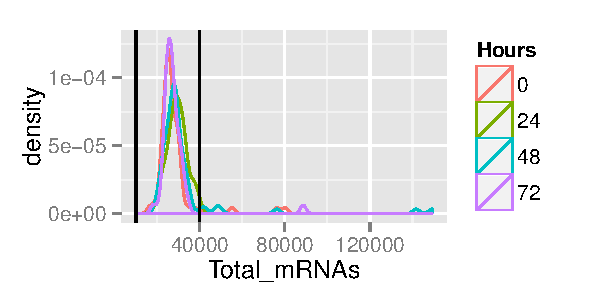
\includegraphics[width=\maxwidth]{figure/show_mRNA_totals-1} 

}


\begin{kframe}\begin{alltt}
\hlstd{HSMM} \hlkwb{<-} \hlstd{HSMM[,}\hlkwd{pData}\hlstd{(HSMM)}\hlopt{$}\hlstd{Total_mRNAs} \hlopt{>} \hlstd{lower_bound} \hlopt{&}
             \hlkwd{pData}\hlstd{(HSMM)}\hlopt{$}\hlstd{Total_mRNAs} \hlopt{<} \hlstd{upper_bound]}
\hlstd{HSMM} \hlkwb{<-} \hlkwd{detectGenes}\hlstd{(HSMM,} \hlkwc{min_expr} \hlstd{=} \hlnum{0.1}\hlstd{)}
\end{alltt}
\end{kframe}
\end{knitrout}
 
 We've gone ahead and removed the few cells with either very low mRNA recovery or far more mRNA that the typical cell. Often, doublets or triplets have roughly twice the mRNA recovered as true single cells, so the latter filter is another means of excluding all but single cells from the analysis. Such filtering is handy if your protocol doesn't allow directly visualization of cell after they've been captured. Note that these thresholds of 10,000 and 40,000 mRNAs are specific to this dataset. You may need to adjust filter thresholds based on your experimental protocol.
 
 Once you've excluded cells that do not pass your quality control filters, you should verify that the expression values stored in your \Rclass{CellDataSet} follow a distribution that is roughly lognormal:  
\begin{knitrout}
\definecolor{shadecolor}{rgb}{0.969, 0.969, 0.969}\color{fgcolor}\begin{kframe}
\begin{alltt}
\hlcom{# Log-transform each value in the expression matrix.}
\hlstd{L} \hlkwb{<-} \hlkwd{log}\hlstd{(}\hlkwd{exprs}\hlstd{(HSMM[expressed_genes,]))}

\hlcom{# Standardize each gene, so that they are all on the same scale,}
\hlcom{# Then melt the data with plyr so we can plot it easily"}
\hlstd{melted_dens_df} \hlkwb{<-} \hlkwd{melt}\hlstd{(Matrix}\hlopt{::}\hlkwd{t}\hlstd{(}\hlkwd{scale}\hlstd{(Matrix}\hlopt{::}\hlkwd{t}\hlstd{(L))))}

\hlcom{# Plot the distribution of the standardized gene expression values.}
\hlkwd{qplot}\hlstd{(value,} \hlkwc{geom}\hlstd{=}\hlstr{"density"}\hlstd{,} \hlkwc{data}\hlstd{=melted_dens_df)} \hlopt{+}  \hlkwd{stat_function}\hlstd{(}\hlkwc{fun} \hlstd{= dnorm,} \hlkwc{size}\hlstd{=}\hlnum{0.5}\hlstd{,} \hlkwc{color}\hlstd{=}\hlstr{'red'}\hlstd{)} \hlopt{+}
  \hlkwd{xlab}\hlstd{(}\hlstr{"Standardized log(FPKM)"}\hlstd{)} \hlopt{+}
  \hlkwd{ylab}\hlstd{(}\hlstr{"Density"}\hlstd{)}
\end{alltt}
\end{kframe}

{\centering 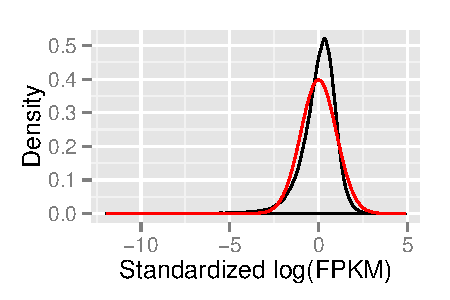
\includegraphics[width=\maxwidth]{figure/lognormal_plot-1} 

}



\end{knitrout}
 
 \section{Classifying and counting cells of different types}
 
 Single cell experiments are often performed on complex mixtures of multiple cell types. Dissociated tissue samples might contain two, three, or even many different cells types. In such cases, it's often nice to classify cells based on type using known markers. In the myoblast experiment, the culture contains fibroblasts that came from the original muscle biopsy used to establish the primary cell culture.  Myoblasts express some key genes that fibroblasts don't. Selecting only the genes that express, for example, sufficiently high levels of \emph{MYF5} excludes the fibroblasts. Likewise, fibroblasts express high levels of \emph{ANPEP} (CD13), while myoblasts tend to express few if any transcripts of this gene. 
 
 \subsection{Classifying cells with CellTypeHierarchy}
 Monocle provides a simple system for tagging cells based on the expression of marker genes of your choosing. You simply provide a set of functions that Monocle can use to annotate each cell. For example, you could provide a function for each of several cell types. These functions accept as input the expression data for each cell, and return TRUE to tell Monocle that a cell meets the criteria defined by the function. So you could have one function that returns TRUE for cells that express myoblast-specific genes, another function for fibroblast-specific genes, etc. Here's an example of such a set of ``gating'' functions:
 
\begin{knitrout}
\definecolor{shadecolor}{rgb}{0.969, 0.969, 0.969}\color{fgcolor}\begin{kframe}
\begin{alltt}
\hlstd{MYF5_id} \hlkwb{<-} \hlkwd{row.names}\hlstd{(}\hlkwd{subset}\hlstd{(}\hlkwd{fData}\hlstd{(HSMM), gene_short_name} \hlopt{==} \hlstr{"MYF5"}\hlstd{))}
\hlstd{ANPEP_id} \hlkwb{<-} \hlkwd{row.names}\hlstd{(}\hlkwd{subset}\hlstd{(}\hlkwd{fData}\hlstd{(HSMM), gene_short_name} \hlopt{==} \hlstr{"ANPEP"}\hlstd{))}

\hlstd{cth} \hlkwb{<-} \hlkwd{newCellTypeHierarchy}\hlstd{()}
\hlstd{cth} \hlkwb{<-} \hlkwd{addCellType}\hlstd{(cth,} \hlstr{"Myoblast"}\hlstd{,} \hlkwc{classify_func}\hlstd{=}\hlkwa{function}\hlstd{(}\hlkwc{x}\hlstd{) \{x[MYF5_id,]} \hlopt{>=} \hlnum{1}\hlstd{\})}
\hlstd{cth} \hlkwb{<-} \hlkwd{addCellType}\hlstd{(cth,} \hlstr{"Fibroblast"}\hlstd{,} \hlkwc{classify_func}\hlstd{=}\hlkwa{function}\hlstd{(}\hlkwc{x}\hlstd{)}
       \hlstd{\{x[MYF5_id,]} \hlopt{<} \hlnum{1} \hlopt{&} \hlstd{x[ANPEP_id,]} \hlopt{>} \hlnum{1}\hlstd{\})}
\end{alltt}
\end{kframe}
\end{knitrout}
 
 The functions are organized into a small data structure called a \Robject{CellTypeHierarchy}, that Monocle uses to classify the cells. You first initialize a new CellTypeHierarchy object, then register your gating functions within it. Once the data structure is set up, you can use it to classify all the cells in the experiment:
 
\begin{knitrout}
\definecolor{shadecolor}{rgb}{0.969, 0.969, 0.969}\color{fgcolor}\begin{kframe}
\begin{alltt}
\hlstd{HSMM} \hlkwb{<-} \hlkwd{classifyCells}\hlstd{(HSMM, cth,} \hlnum{0.1}\hlstd{)}
\end{alltt}
\end{kframe}
\end{knitrout}
 
 The function \Rfunction{classifyCells} applies each gating function to each cell, classifies the cells according to the gating functions, and returns the \Robject{CellDataSet} with a new column, \Robject{CellType} in its \Robject{pData} table. We can now count how many cells of each type there are in the experiment.
 
\begin{knitrout}
\definecolor{shadecolor}{rgb}{0.969, 0.969, 0.969}\color{fgcolor}\begin{kframe}
\begin{alltt}
\hlkwd{table}\hlstd{(}\hlkwd{pData}\hlstd{(HSMM)}\hlopt{$}\hlstd{CellType)}
\end{alltt}
\begin{verbatim}
## 
## Fibroblast   Myoblast    Unknown 
##         56         85        121
\end{verbatim}
\begin{alltt}
\hlstd{pie} \hlkwb{<-} \hlkwd{ggplot}\hlstd{(}\hlkwd{pData}\hlstd{(HSMM),} \hlkwd{aes}\hlstd{(}\hlkwc{x} \hlstd{=} \hlkwd{factor}\hlstd{(}\hlnum{1}\hlstd{),} \hlkwc{fill} \hlstd{=} \hlkwd{factor}\hlstd{(CellType)))} \hlopt{+}
  \hlkwd{geom_bar}\hlstd{(}\hlkwc{width} \hlstd{=} \hlnum{1}\hlstd{)}
\hlstd{pie} \hlopt{+} \hlkwd{coord_polar}\hlstd{(}\hlkwc{theta} \hlstd{=} \hlstr{"y"}\hlstd{)} \hlopt{+}
  \hlkwd{theme}\hlstd{(}\hlkwc{axis.title.x}\hlstd{=}\hlkwd{element_blank}\hlstd{(),} \hlkwc{axis.title.y}\hlstd{=}\hlkwd{element_blank}\hlstd{())}
\end{alltt}
\end{kframe}

{\centering 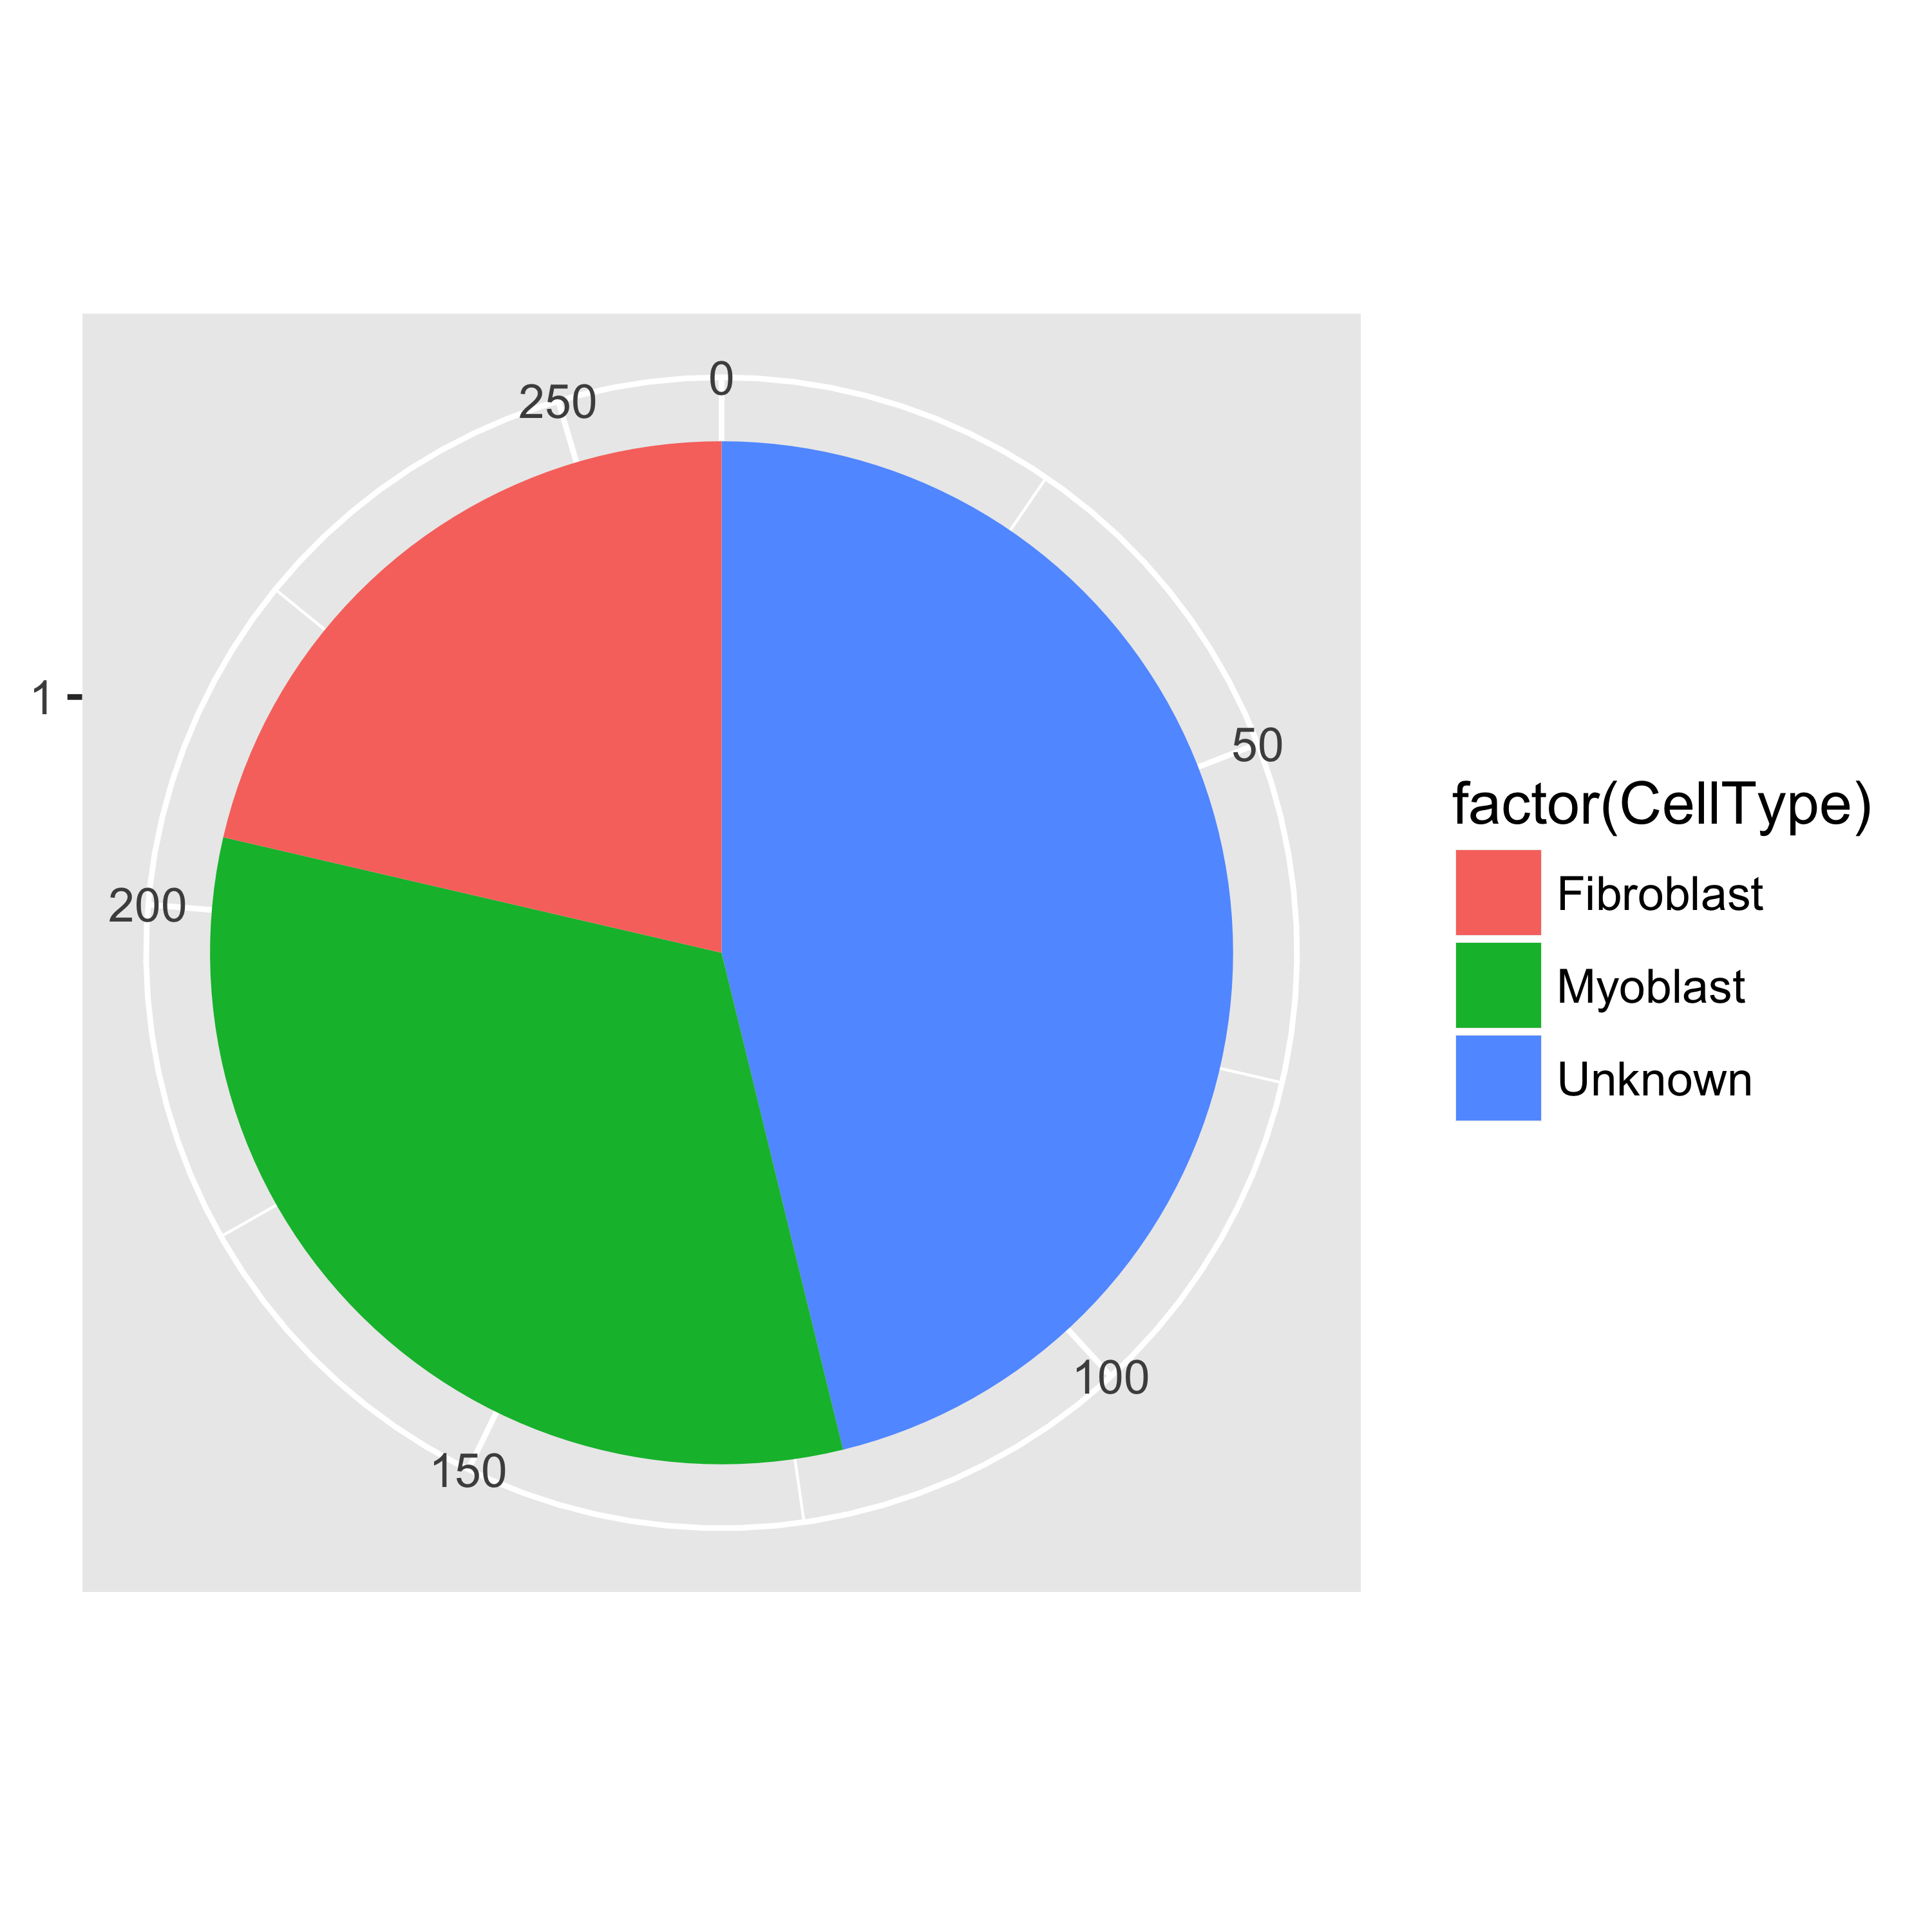
\includegraphics[width=\maxwidth]{figure/count_cells_unsup_readout-1} 

}



\end{knitrout}
 
 Note that many cells are marked ``Unknown''. This is common, largely because of the low rate of mRNA capture in most single-cell RNA-Seq experiments. A cell might express a few \emph{MYF5} mRNAs, but we weren't lucky enough to capture one of them. When a cell doesn't meet any of the criteria specified in your classification functions, it's marked ``Unknown''. If it meets multiple functions' criteria, it's marked ``Ambiguous''. You could just exclude such cells, but you'd be throwing out a lot of your data. In this case, we'd lose more than half of the cells!

\subsection{Unsupervised cell clustering}
Monocle provides an algorithm you can use to impute the types of the ``Unknown'' cells. This algorithm, implemented in the function \Rfunction{clusterCells}, groups cells together according to global expression profile. That way, if your cell expresses lots of genes specific to myoblasts, but just happens to lack \emph{MYF5}, we can still recognize it as a myoblast. \Rfunction{clusterCells} can be used in an unsupervised manner, as well as in a ``semi-supervised'' mode, which allows to assist the algorithm with some expert knowledge. Let's look at the unsupervised mode first.

The first step is to decide which genes to use in clustering the cells. We could use all genes, but we'd be including a lot of genes that are not expressed at a high enough level to provide a meaningful signal. Including them would just add noise to the system. We can filter genes based on average expression level, and we can additionally select genes that are unusually variable across cells. These genes tend to be highly informative about cell state.

\begin{knitrout}
\definecolor{shadecolor}{rgb}{0.969, 0.969, 0.969}\color{fgcolor}\begin{kframe}
\begin{alltt}
\hlstd{disp_table} \hlkwb{<-} \hlkwd{dispersionTable}\hlstd{(HSMM)}
\hlstd{unsup_clustering_genes} \hlkwb{<-} \hlkwd{subset}\hlstd{(disp_table, mean_expression} \hlopt{>=} \hlnum{0.1}\hlstd{)}
\hlstd{HSMM} \hlkwb{<-} \hlkwd{setOrderingFilter}\hlstd{(HSMM, unsup_clustering_genes}\hlopt{$}\hlstd{gene_id)}
\hlkwd{plot_ordering_genes}\hlstd{(HSMM)}
\end{alltt}
\end{kframe}

{\centering 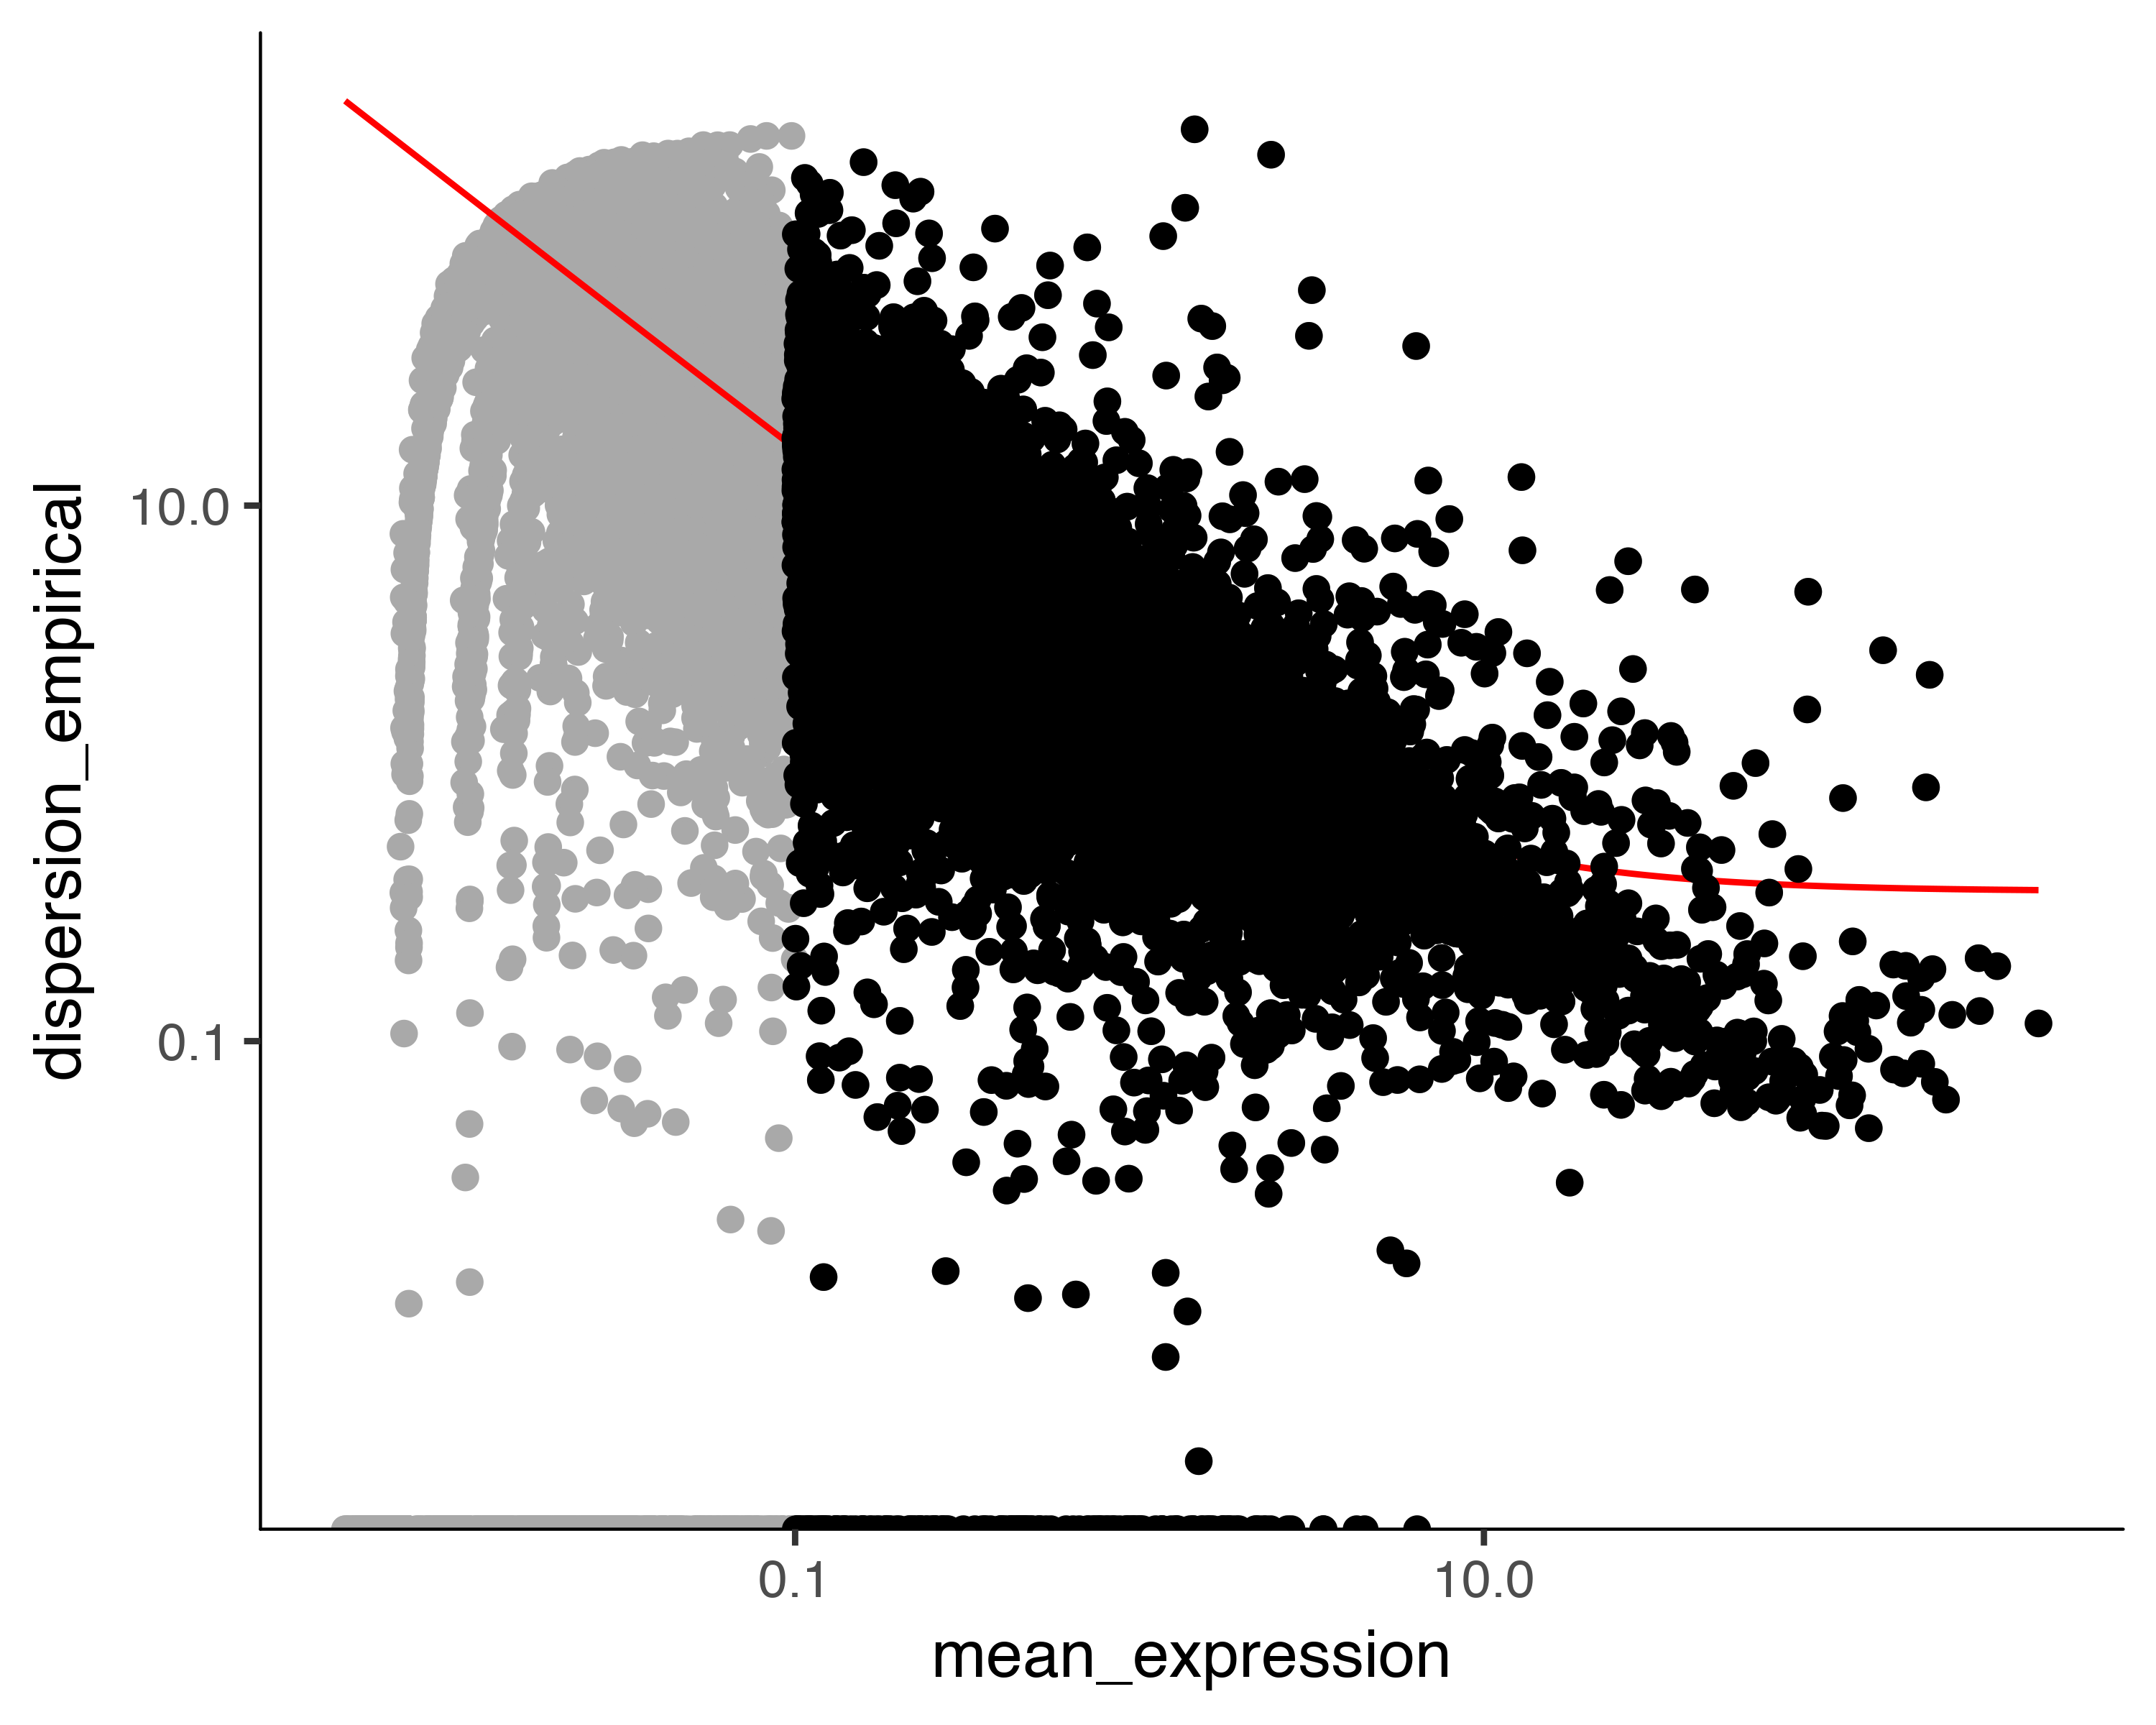
\includegraphics[width=\maxwidth]{figure/cluster_cells_unsup_gene_pick-1} 

}



\end{knitrout}

The \Rfunction{setOrderingFilter} function marks genes that will be used for clustering in subsequent calls to \Rfunction{clusterCells}, although we will be able to provide other lists of genes if we want. \Rfunction{plot\_ordering\_genes} shows how variability (dispersion) in a gene's expression depends on the average expression across cells. The red line shows Monocle's expectation of the dispersion based on this relationship. The genes we marked for use in clustering are shown as black dots, while the others are shown as grey dots.

Now we're ready to try clustering the cells:

\begin{knitrout}
\definecolor{shadecolor}{rgb}{0.969, 0.969, 0.969}\color{fgcolor}\begin{kframe}
\begin{alltt}
\hlcom{# HSMM@auxClusteringData[["tSNE"]]$variance_explained <- NULL}
\hlkwd{plot_pc_variance_explained}\hlstd{(HSMM,} \hlkwc{return_all} \hlstd{= F)} \hlcom{# norm_method = 'log',}
\end{alltt}
\end{kframe}

{\centering 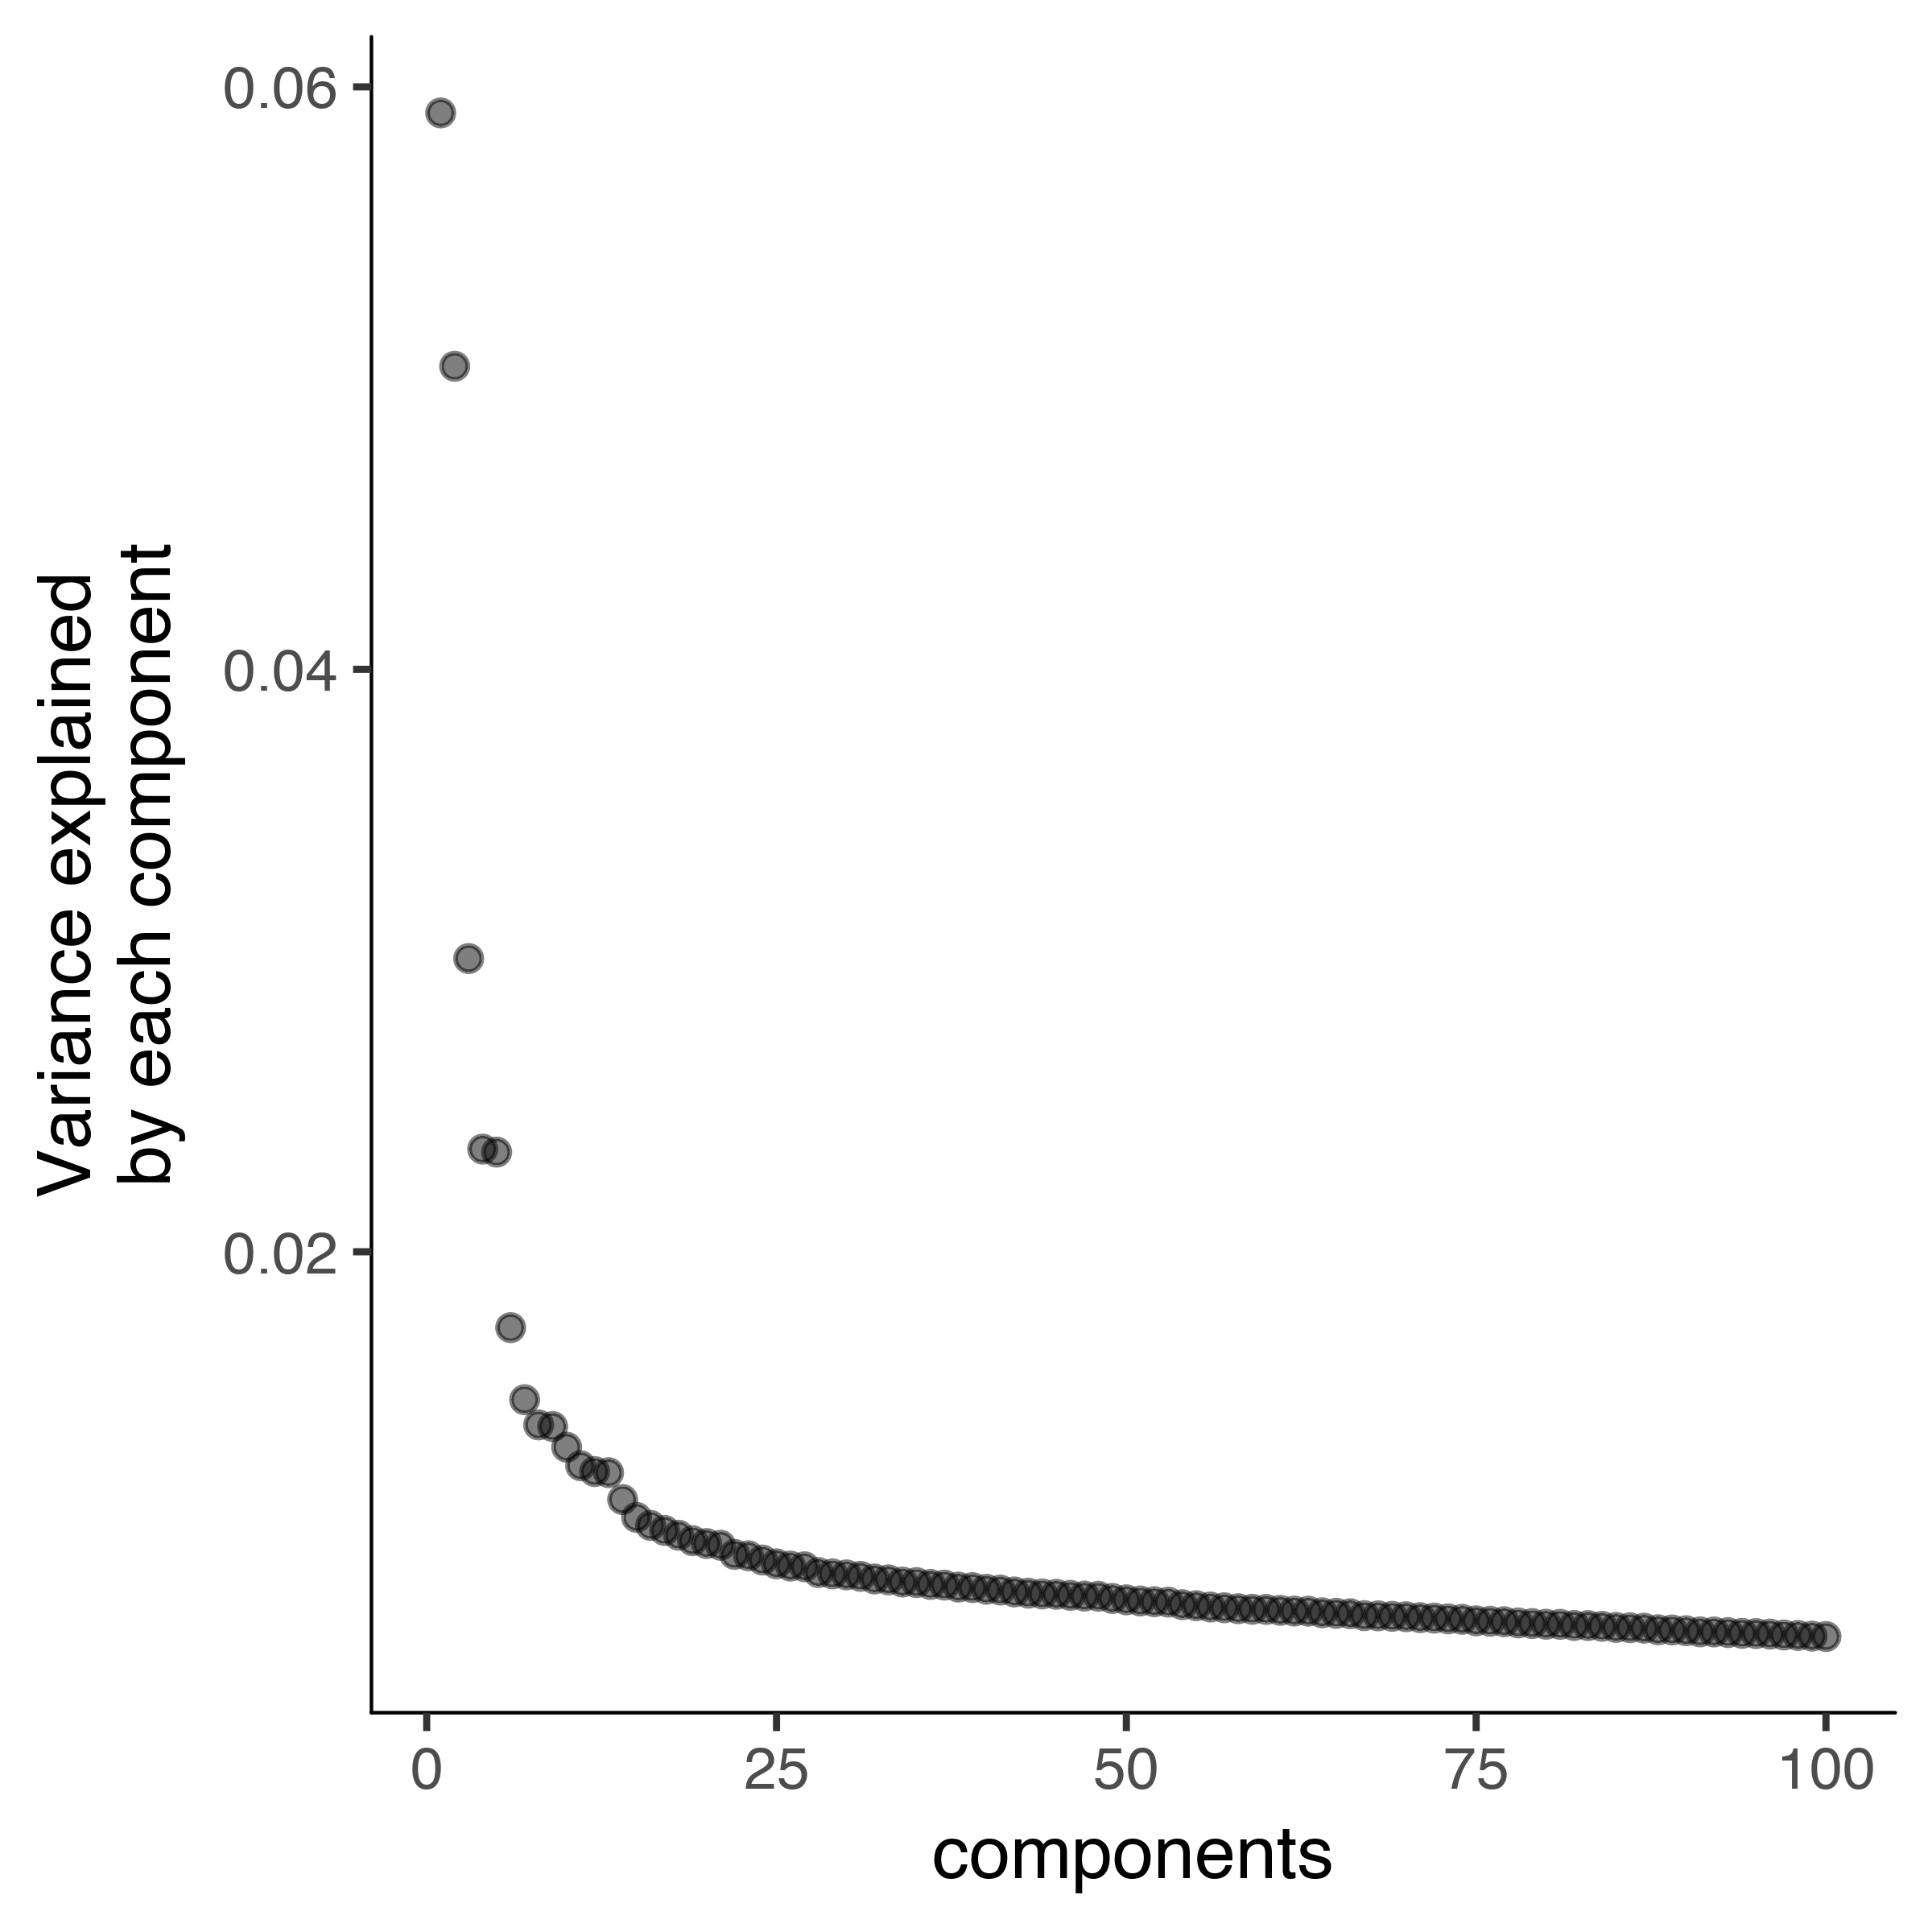
\includegraphics[width=\maxwidth]{figure/cluster_cells_unsup_no_covariate-1} 

}


\begin{kframe}\begin{alltt}
\hlstd{HSMM} \hlkwb{<-} \hlkwd{reduceDimension}\hlstd{(HSMM,} \hlkwc{max_components}\hlstd{=}\hlnum{2}\hlstd{,} \hlkwc{num_dim} \hlstd{=} \hlnum{6}\hlstd{,}
                        \hlkwc{reduction_method} \hlstd{=} \hlstr{'tSNE'}\hlstd{,} \hlkwc{verbose} \hlstd{= T)}
\end{alltt}


{\ttfamily\noindent\itshape\color{messagecolor}{\#\# Remove noise by PCA ...}}

{\ttfamily\noindent\itshape\color{messagecolor}{\#\# Reduce dimension by tSNE ...}}\begin{alltt}
\hlstd{HSMM} \hlkwb{<-} \hlkwd{clusterCells}\hlstd{(HSMM,}
                     \hlkwc{num_clusters}\hlstd{=}\hlnum{2}\hlstd{)}
\end{alltt}
\begin{verbatim}
## Distance cutoff calculated to 1.12138
\end{verbatim}


{\ttfamily\noindent\itshape\color{messagecolor}{\#\# the length of the distance: 34191}}\begin{alltt}
\hlkwd{plot_cell_clusters}\hlstd{(HSMM,} \hlnum{1}\hlstd{,} \hlnum{2}\hlstd{,} \hlkwc{color}\hlstd{=}\hlstr{"CellType"}\hlstd{,} \hlkwc{markers}\hlstd{=}\hlkwd{c}\hlstd{(}\hlstr{"MYF5"}\hlstd{,} \hlstr{"ANPEP"}\hlstd{))}
\end{alltt}
\end{kframe}

{\centering 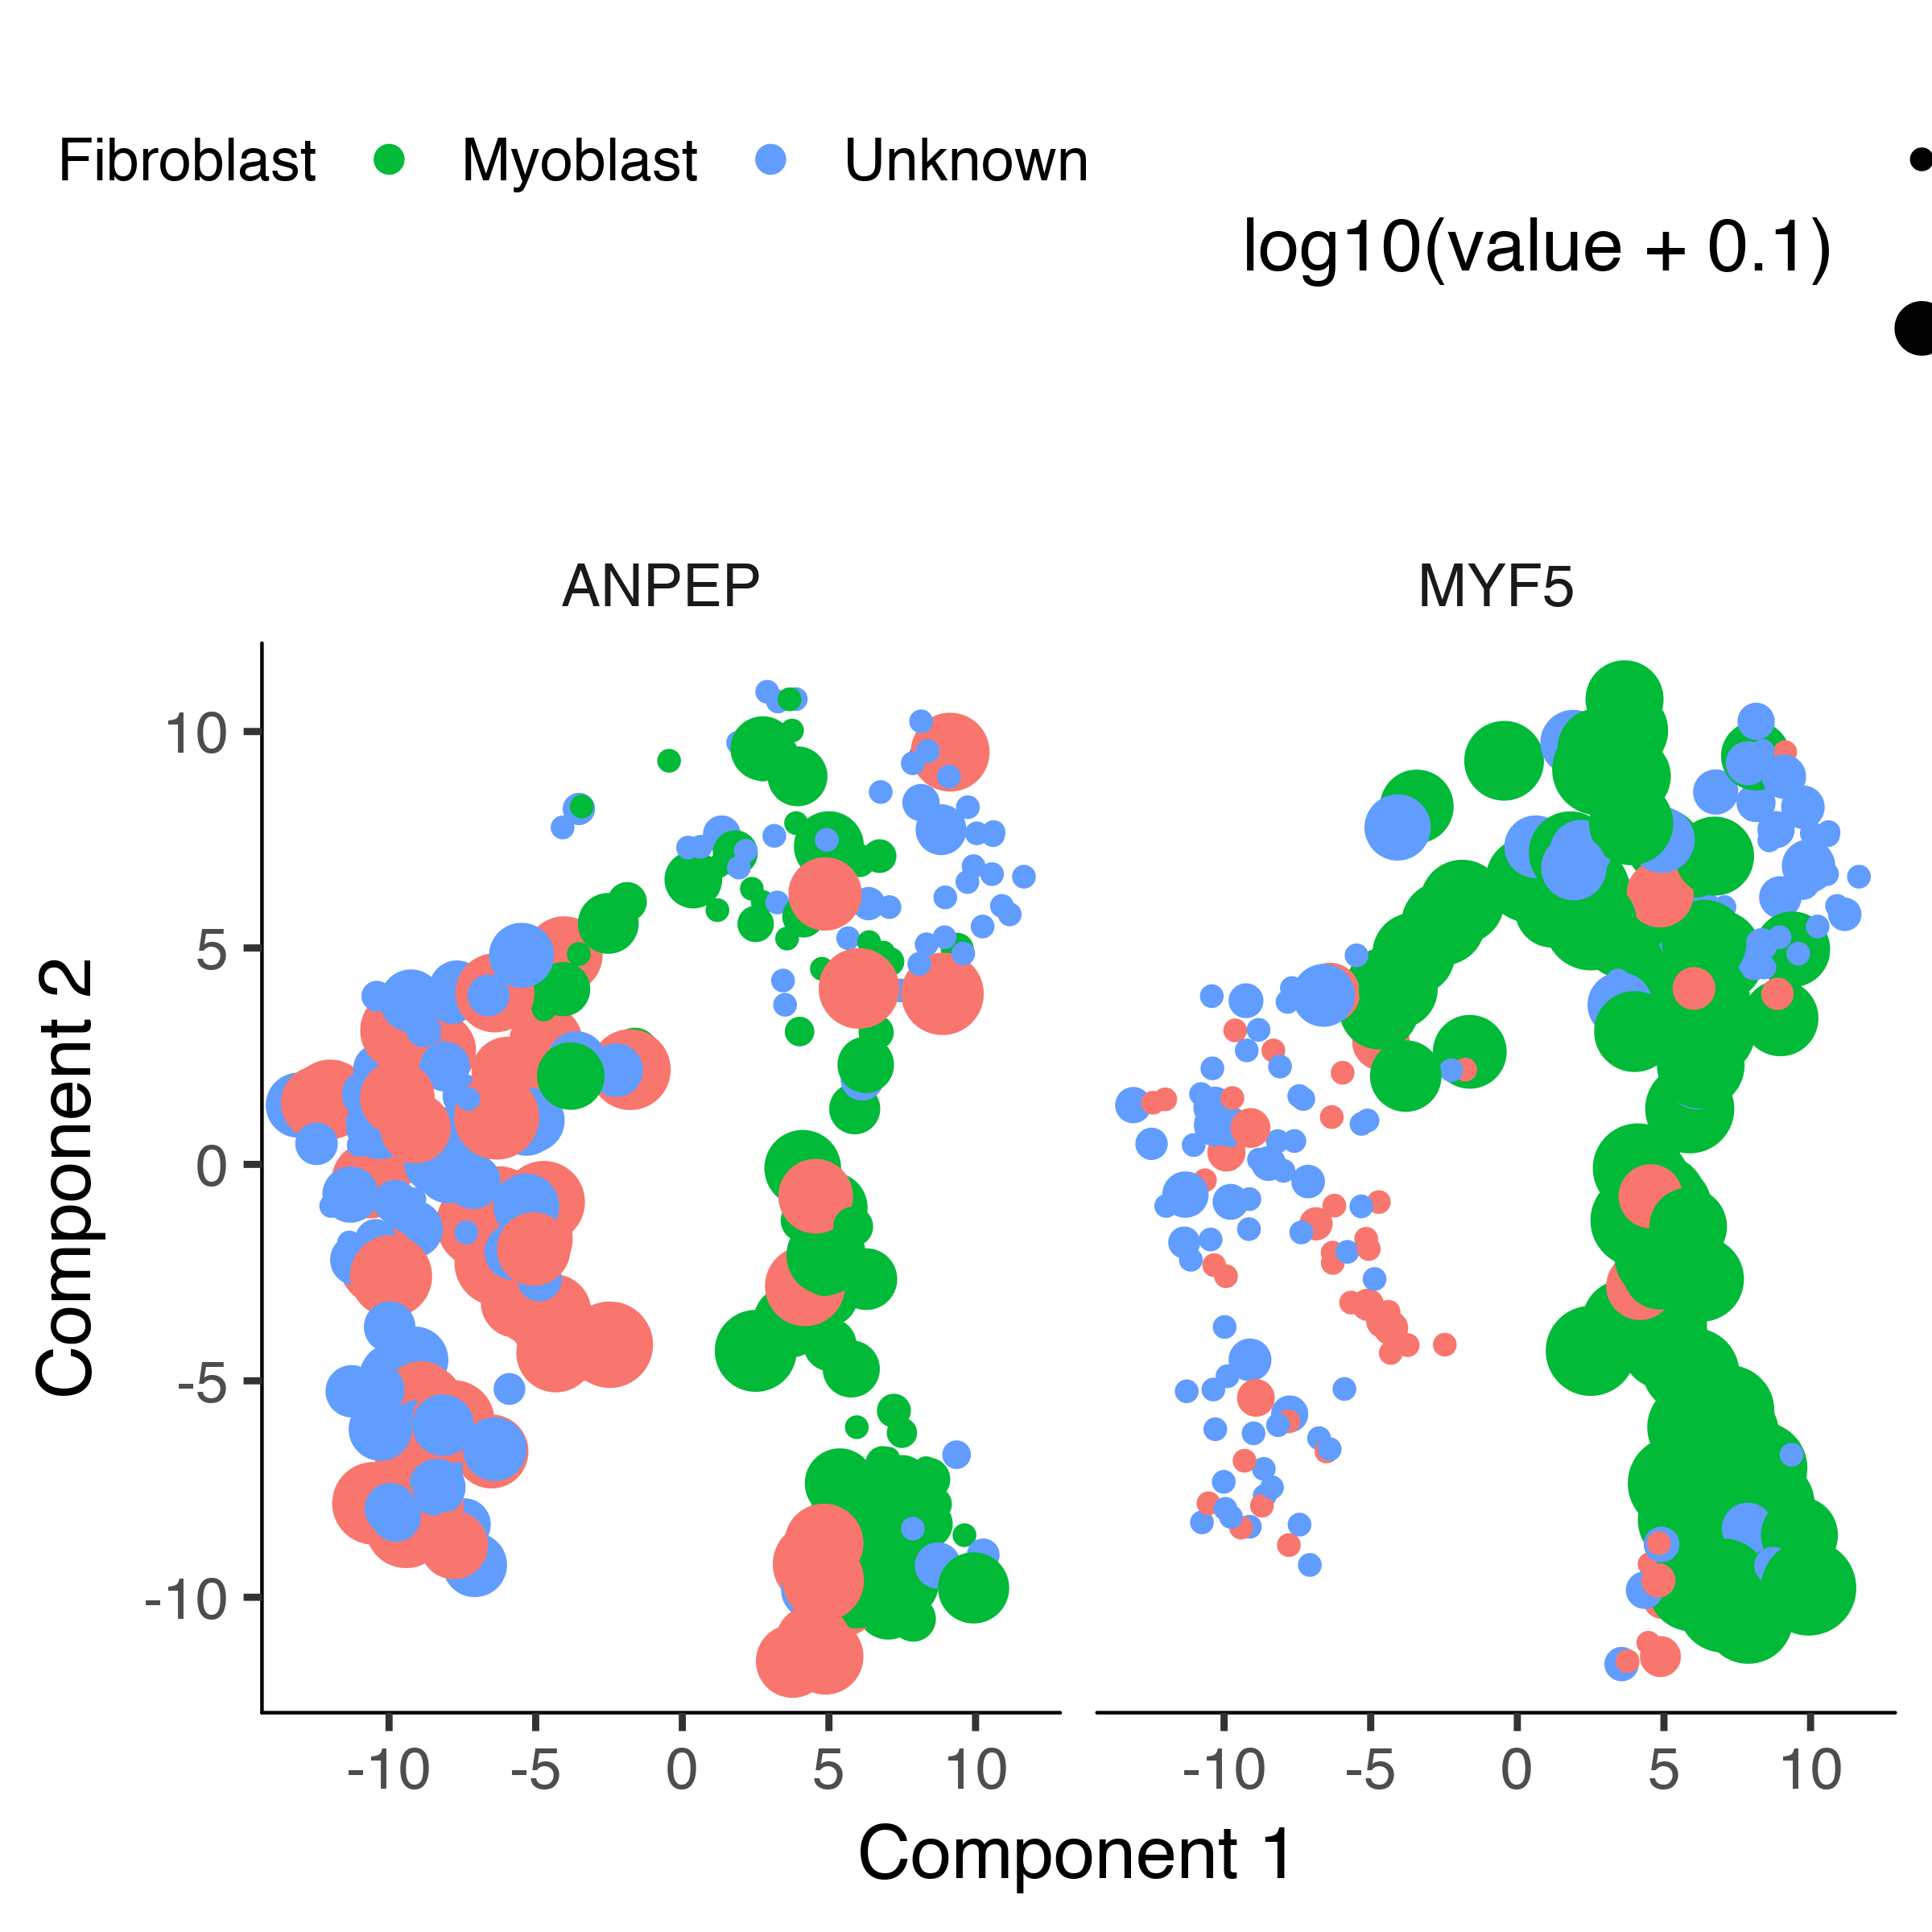
\includegraphics[width=\maxwidth]{figure/cluster_cells_unsup_no_covariate-2} 

}



\end{knitrout}

Monocle uses t-SNE \cite{Maaten2008-om} to cluster cells, using an approach that's very similar to and inspired by Rahul Satija's excellent \href{http://satijalab.org/seurat/}{Seurat} package, which itself was inspired by \href{https://www.c2b2.columbia.edu/danapeerlab/html/cyt.html}{viSNE} from Dana Pe'er's lab.

The cells tagged as myoblasts by our gating functions are marked in green, while the fibroblasts are tagged in red. The cells that don't express either marker are blue. In many experiments, cells of different types are clearly separate from one another. Unfortunately, in this experiment, the cells don't simply cluster by type - there's not a clear space between the green cells and the red cells. This isn't all that surprising, because myoblasts and contaminating interstitial fibroblasts express many of the same genes in these culture conditions, and there are multiple culture conditions in the experiment. That is, there are other sources of variation in the experiment that might be driving the clustering. One source of variation in the experiment stems from the experimental design. To initiate myoblast differentiation, we switch media from a high-mitogen growth medium (GM) to a low-mitogen differentiation medium (DM). Perhaps the cells are clustering based on the media they're cultured in?

\begin{knitrout}
\definecolor{shadecolor}{rgb}{0.969, 0.969, 0.969}\color{fgcolor}\begin{kframe}
\begin{alltt}
\hlkwd{plot_cell_clusters}\hlstd{(HSMM,} \hlnum{1}\hlstd{,} \hlnum{2}\hlstd{,} \hlkwc{color}\hlstd{=}\hlstr{"Media"}\hlstd{)}
\end{alltt}
\end{kframe}

{\centering 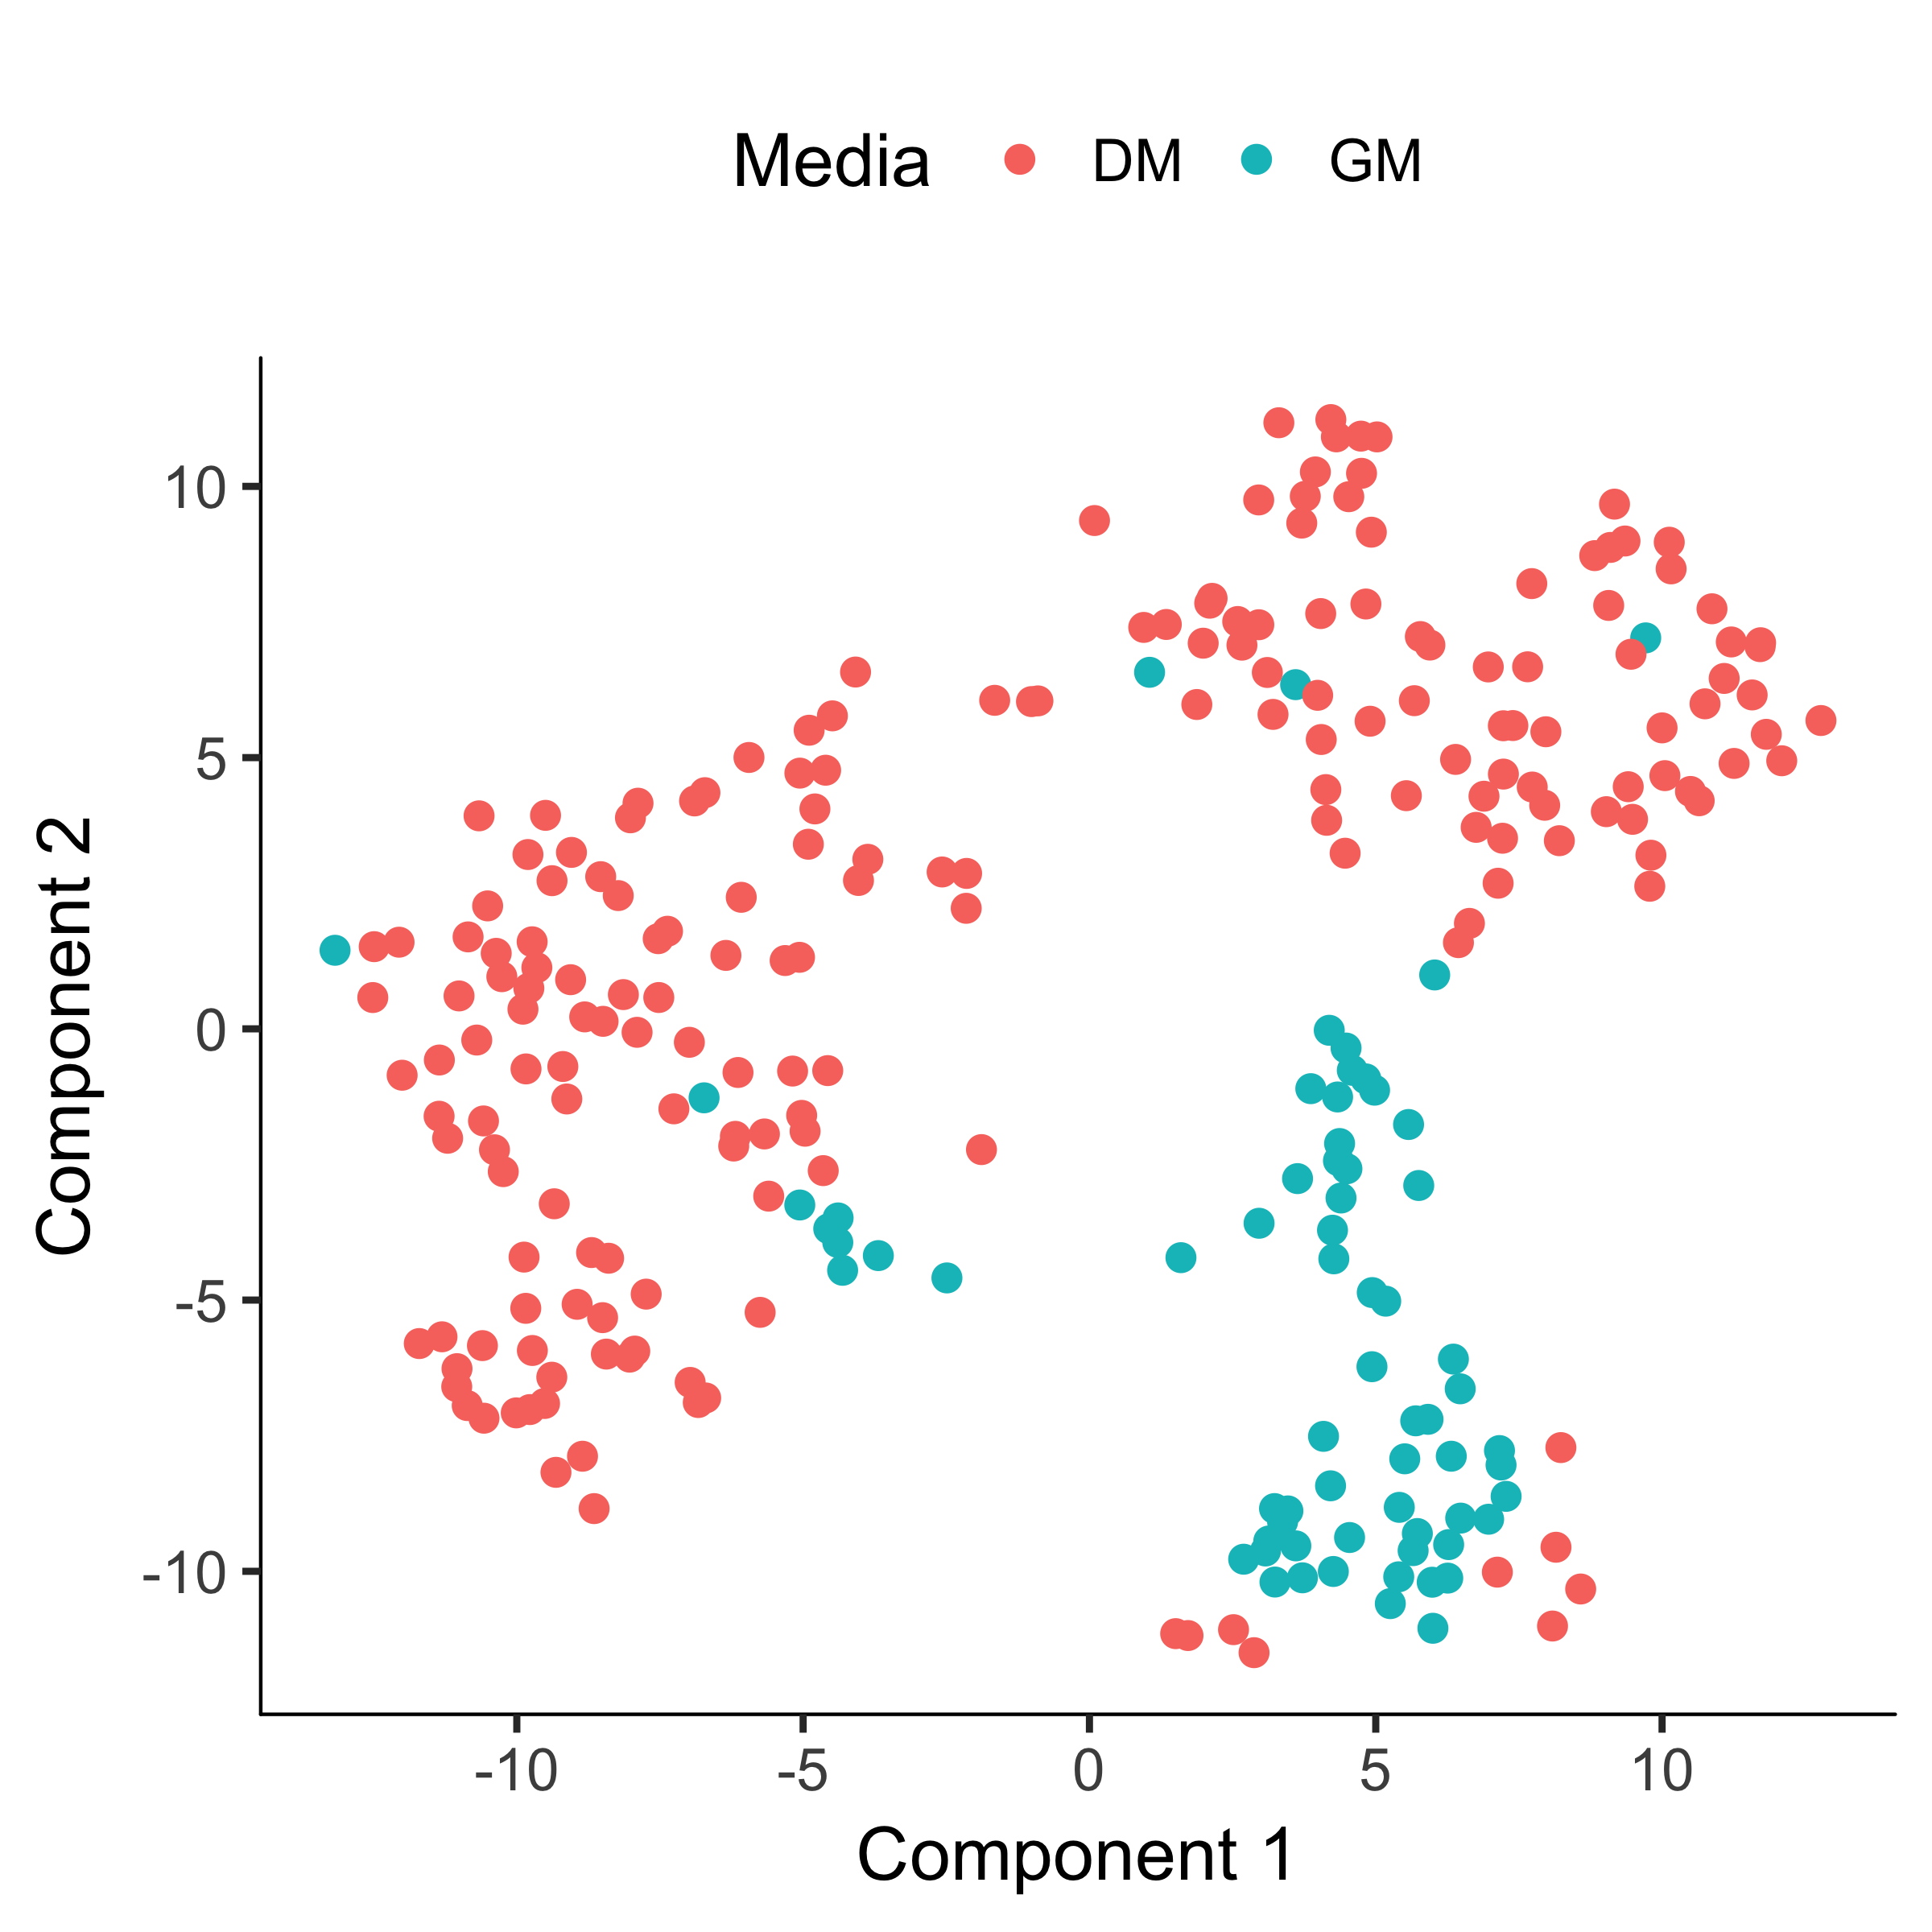
\includegraphics[width=\maxwidth]{figure/cluster_cells_unsup_plot_by_media-1} 

}



\end{knitrout}

Monocle allows us to subtract the effects of ``uninteresting'' sources of variation to reduce their impact on the clustering. You can do this with the \Robject{residualModelFormulaStr} argument to \Rfunction{clusterCells} and several other Monocle functions. This argument accepts an R model formula string specifying the effects you want to subtract prior to clustering.

\begin{knitrout}
\definecolor{shadecolor}{rgb}{0.969, 0.969, 0.969}\color{fgcolor}\begin{kframe}
\begin{alltt}
\hlstd{HSMM} \hlkwb{<-} \hlkwd{reduceDimension}\hlstd{(HSMM,} \hlkwc{max_components}\hlstd{=}\hlnum{2}\hlstd{,} \hlkwc{num_dim} \hlstd{=} \hlnum{2}\hlstd{,} \hlkwc{reduction_method} \hlstd{=} \hlstr{'tSNE'}\hlstd{,}
                       \hlkwc{residualModelFormulaStr}\hlstd{=}\hlstr{"~Media + num_genes_expressed"}\hlstd{,} \hlkwc{verbose} \hlstd{= T)} \hlcom{#}
\end{alltt}


{\ttfamily\noindent\itshape\color{messagecolor}{\#\# Removing batch effects}}

{\ttfamily\noindent\itshape\color{messagecolor}{\#\# Remove noise by PCA ...}}

{\ttfamily\noindent\itshape\color{messagecolor}{\#\# Reduce dimension by tSNE ...}}\begin{alltt}
\hlstd{HSMM} \hlkwb{<-} \hlkwd{clusterCells}\hlstd{(HSMM,} \hlkwc{num_clusters}\hlstd{=}\hlnum{2}\hlstd{)}
\end{alltt}
\begin{verbatim}
## Distance cutoff calculated to 0.9592123
\end{verbatim}


{\ttfamily\noindent\itshape\color{messagecolor}{\#\# the length of the distance: 34191}}\begin{alltt}
\hlkwd{plot_cell_clusters}\hlstd{(HSMM,} \hlnum{1}\hlstd{,} \hlnum{2}\hlstd{,} \hlkwc{color}\hlstd{=}\hlstr{"CellType"}\hlstd{)}
\end{alltt}
\end{kframe}

{\centering 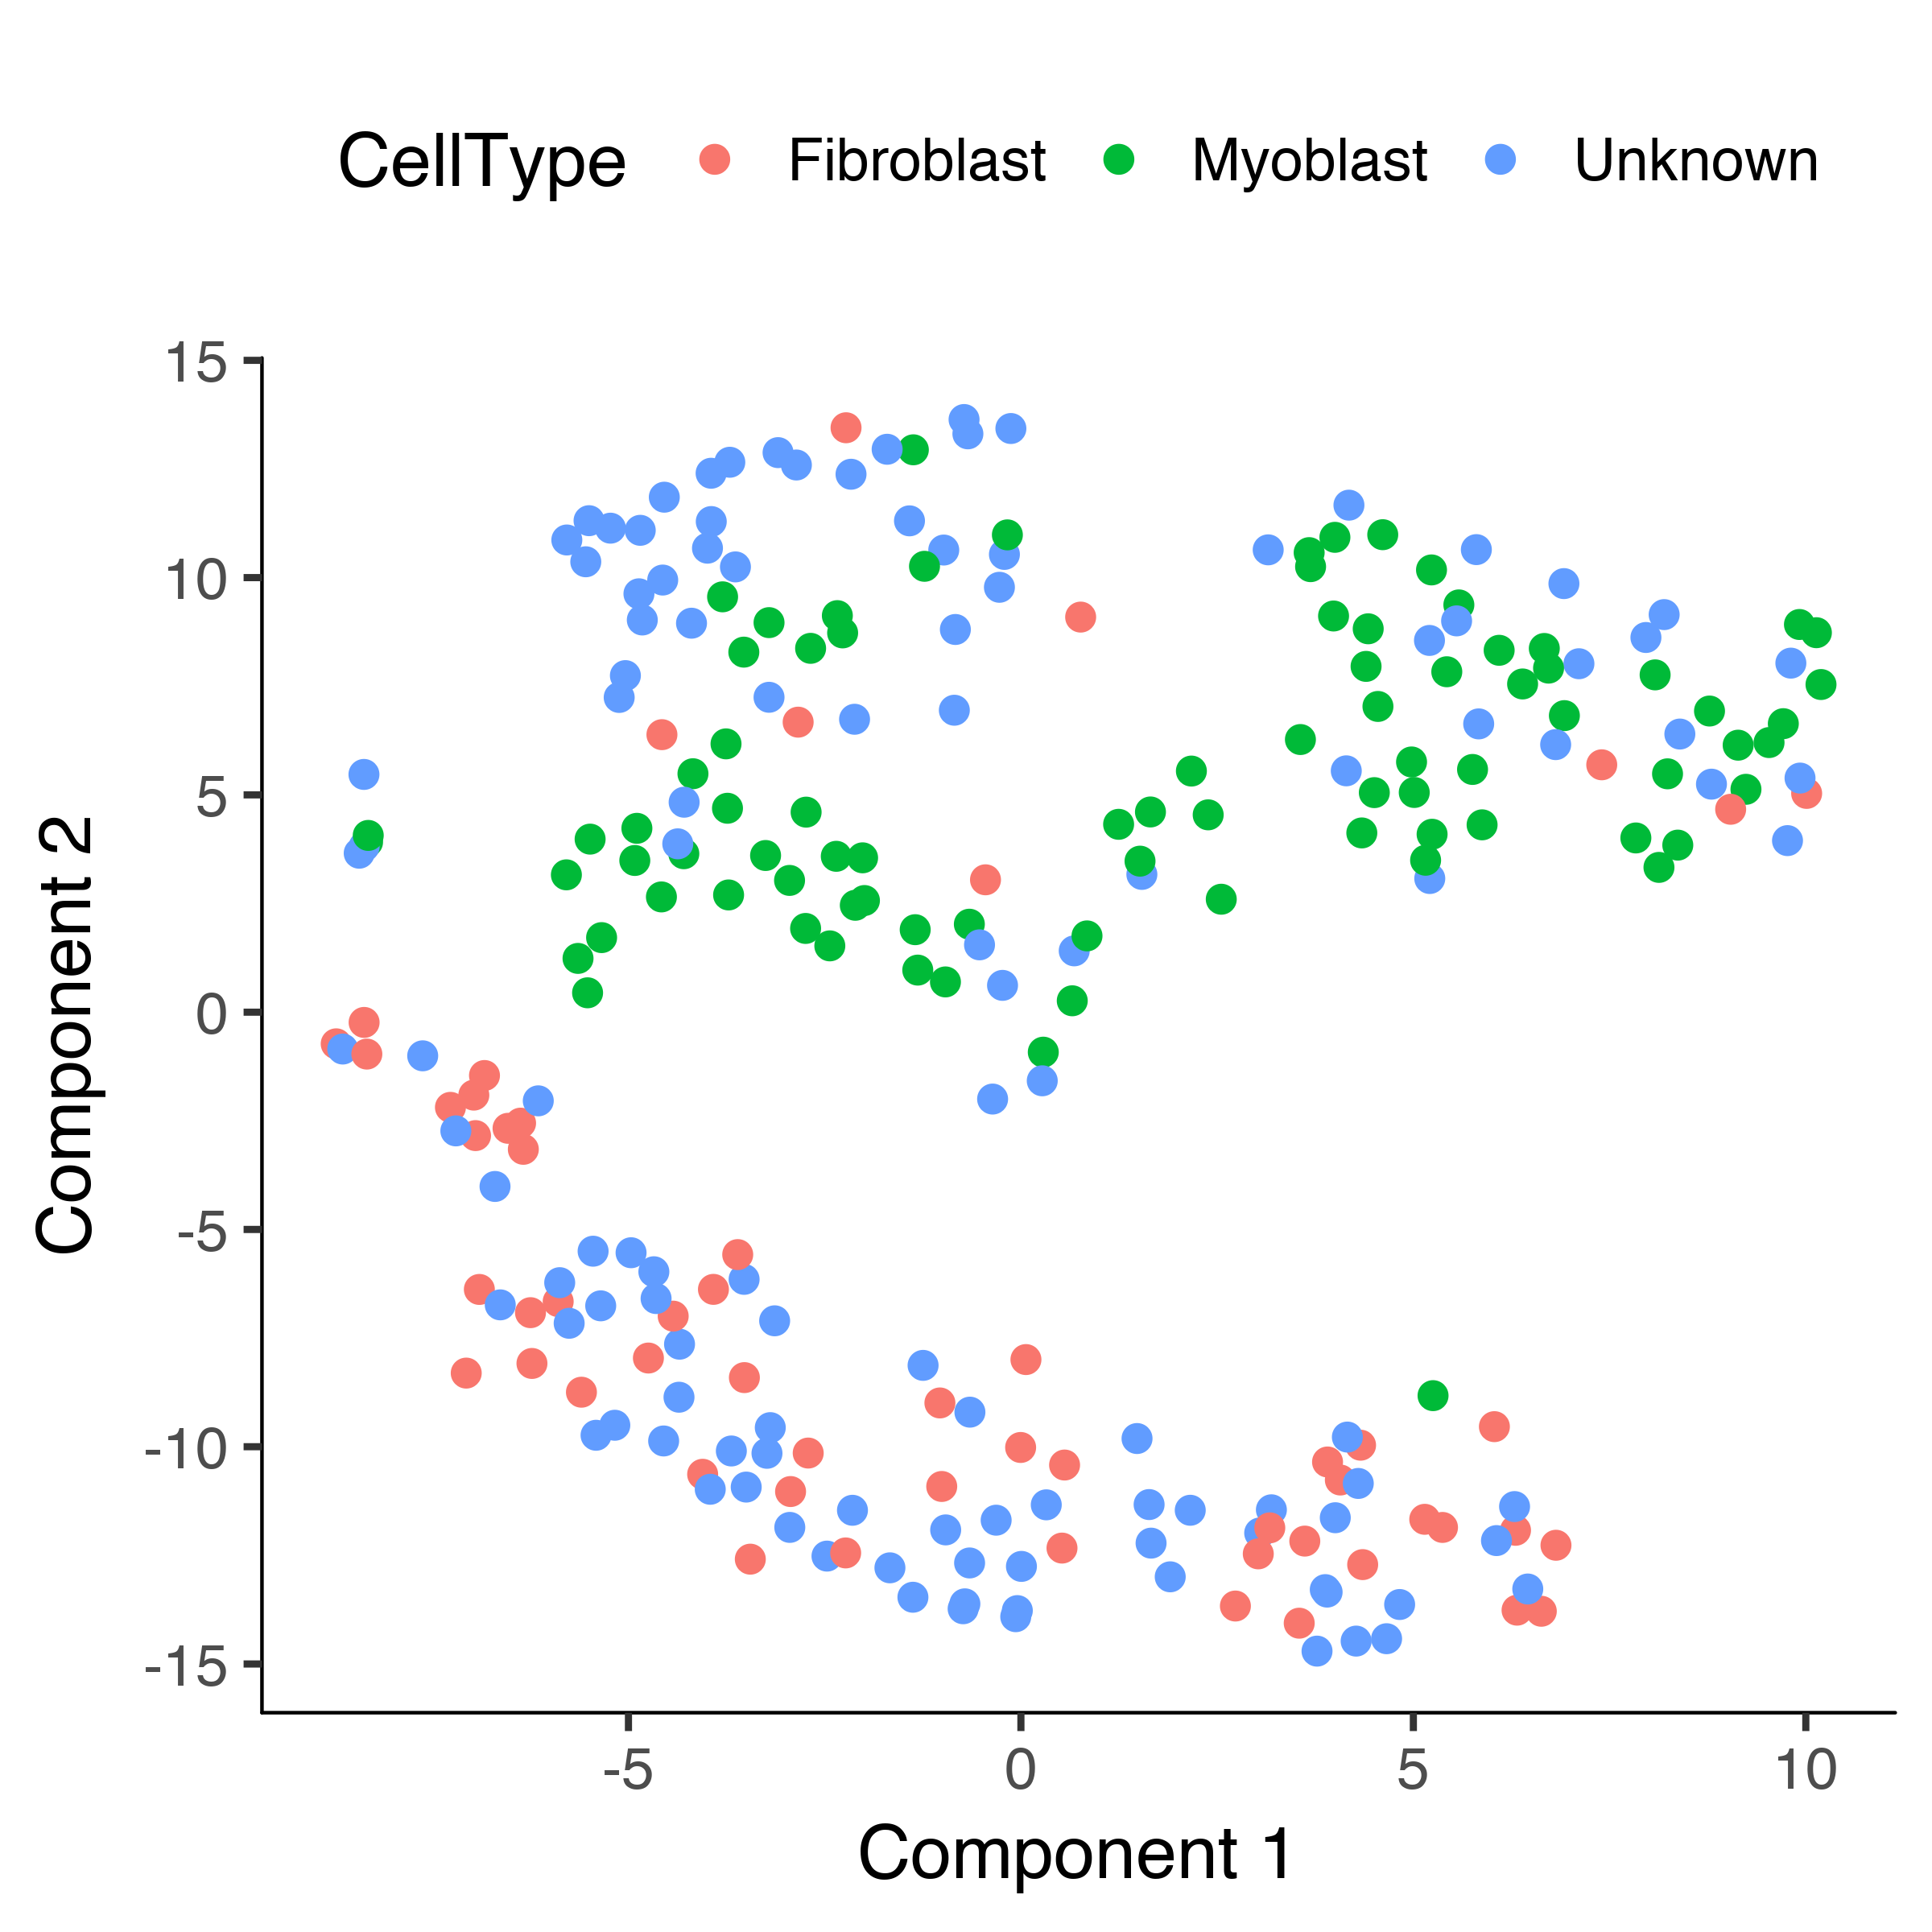
\includegraphics[width=\maxwidth]{figure/cluster_cells_unsup_control_for_media-1} 

}



\end{knitrout}

Now that we've accounted for some unwanted sources of variation, we're ready to take another crack at classifying the cells by unsupervised clustering:

\begin{knitrout}
\definecolor{shadecolor}{rgb}{0.969, 0.969, 0.969}\color{fgcolor}\begin{kframe}
\begin{alltt}
\hlstd{HSMM} \hlkwb{<-} \hlkwd{clusterCells}\hlstd{(HSMM,} \hlkwc{num_clusters}\hlstd{=}\hlnum{2}\hlstd{)}
\end{alltt}
\begin{verbatim}
## Distance cutoff calculated to 0.9592123
\end{verbatim}


{\ttfamily\noindent\itshape\color{messagecolor}{\#\# the length of the distance: 34191}}\begin{alltt}
\hlkwd{plot_cell_clusters}\hlstd{(HSMM,} \hlnum{1}\hlstd{,} \hlnum{2}\hlstd{,} \hlkwc{color}\hlstd{=}\hlstr{"Cluster"}\hlstd{)} \hlopt{+} \hlkwd{facet_wrap}\hlstd{(}\hlopt{~}\hlstd{CellType)}
\end{alltt}
\end{kframe}

{\centering 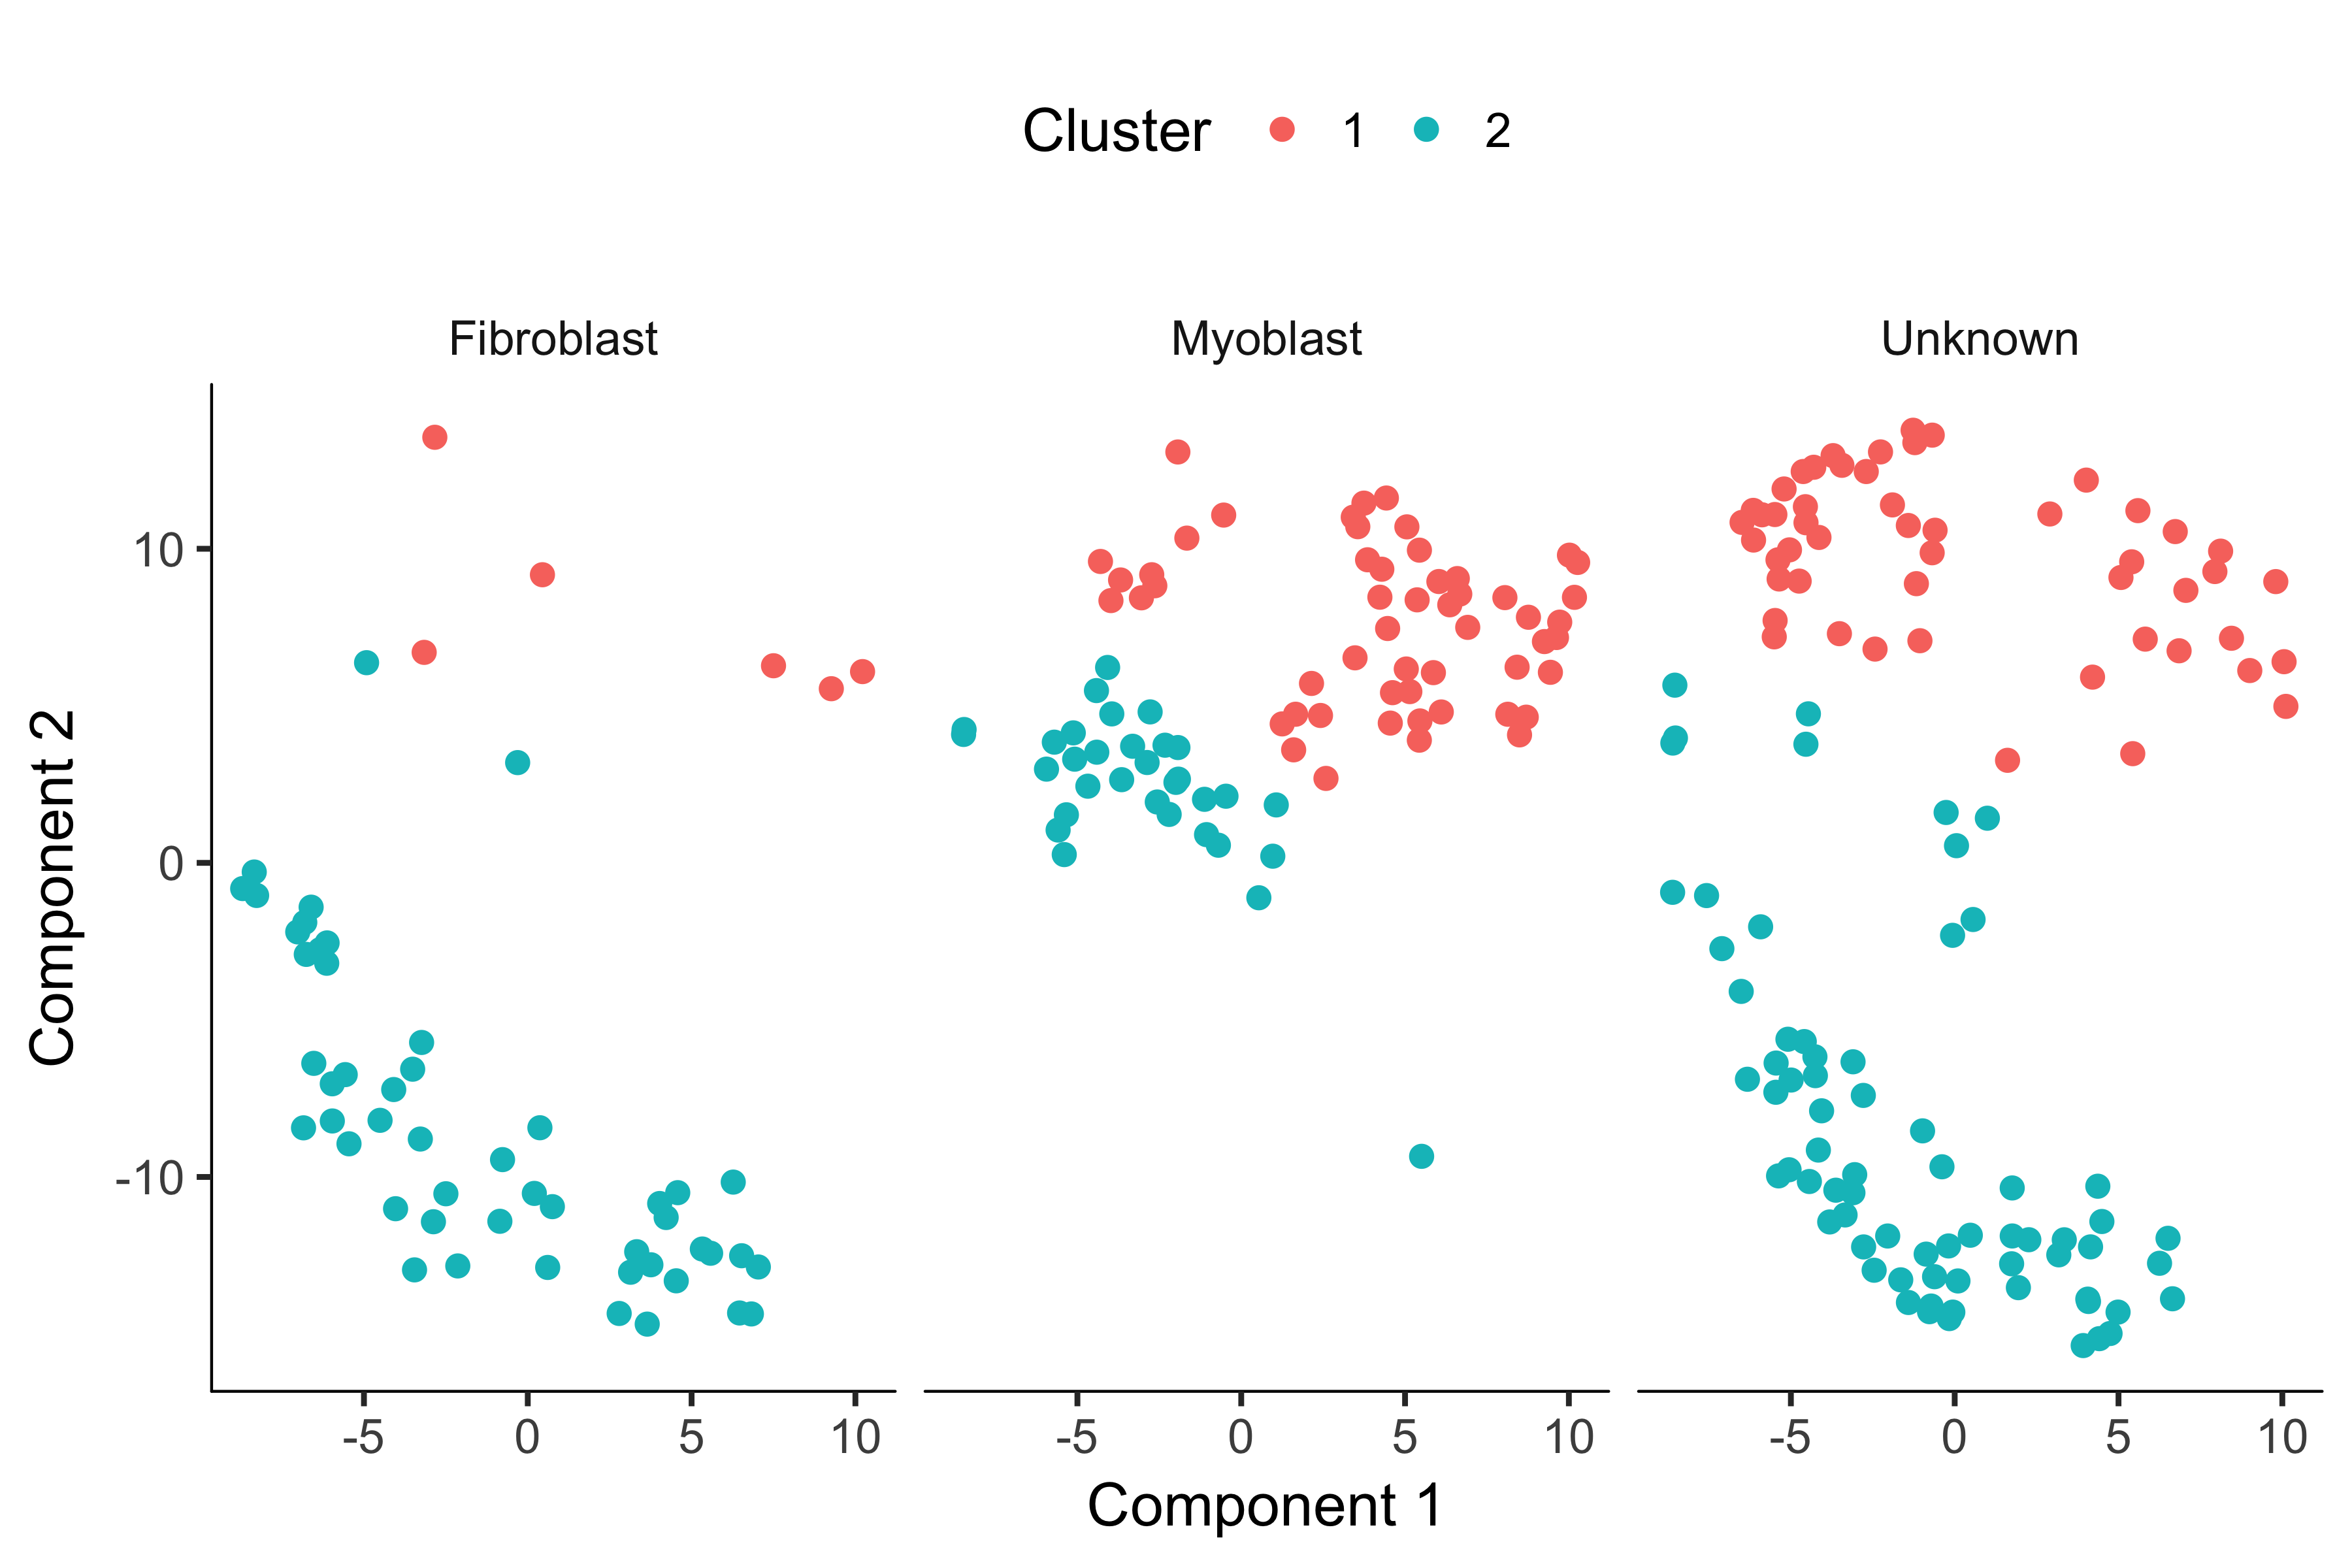
\includegraphics[width=\maxwidth]{figure/cluster_cells_unsup_plot_by_cell_type-1} 

}



\end{knitrout}
 
Now, most of the myoblasts are in one cluster, most of the fibroblasts are in the other, and the unknowns are spread across both. However, we still see some cells of both types in each cluster. This could be due to lack of specificity in our marker genes and our CellTypeHierarchy functions, but it could also be due to suboptimal clustering. To help rule out the latter, let's try running \Rfunction{clusterCells} in its semi-supervised mode.  
  
\subsection{Semi-supervised cell clustering with known marker genes}
  
First, we'll select a different set of genes to use for clustering the cells. Before we just picked genes that were highly expressed and highly variable. Now, we'll pick genes that \emph{co-vary} with our markers. In a sense, we'll be building a large list of genes to use as markers, so that even if a cell doesn't have \emph{MYF5}, it might be recognizable as a myoblast based on other genes.
  
\begin{knitrout}
\definecolor{shadecolor}{rgb}{0.969, 0.969, 0.969}\color{fgcolor}\begin{kframe}
\begin{alltt}
\hlstd{marker_diff} \hlkwb{<-} \hlkwd{markerDiffTable}\hlstd{(HSMM[expressed_genes,],}
                                 \hlstd{cth,}
                                 \hlkwc{residualModelFormulaStr}\hlstd{=}\hlstr{"~Media + num_genes_expressed"}\hlstd{,}
                                 \hlkwc{cores}\hlstd{=}\hlkwd{detectCores}\hlstd{())}
\end{alltt}
\end{kframe}
\end{knitrout}



The function \Rfunction{markerDiffTable} takes a CellDataSet and a CellTypeHierarchy and classifies all the cells into types according to your provided functions. It then removes all the ``Unknown'' and ``Ambiguous'' functions before identifying genes that are differentially expressed between the types. Again, you can provide a residual model of effects to exclude from this test. The function then returns a data frame of test results, and you can use this to pick the genes you want to use for clustering. Often it's best to pick the top 10 or 20 genes that are most specific for each cell type. This ensures that the clustering genes aren't dominated by markers for one cell type. You generally want a balanced panel of markers for each type if possible. Monocle provides a handy function for ranking genes by how restricted their expression is for each type.  


\begin{knitrout}
\definecolor{shadecolor}{rgb}{0.969, 0.969, 0.969}\color{fgcolor}\begin{kframe}
\begin{alltt}
\hlstd{candidate_clustering_genes} \hlkwb{<-} \hlkwd{row.names}\hlstd{(}\hlkwd{subset}\hlstd{(marker_diff, qval} \hlopt{<} \hlnum{0.01}\hlstd{))}
\hlstd{marker_spec} \hlkwb{<-} \hlkwd{calculateMarkerSpecificity}\hlstd{(HSMM[candidate_clustering_genes,], cth)}
\hlkwd{head}\hlstd{(}\hlkwd{selectTopMarkers}\hlstd{(marker_spec,} \hlnum{3}\hlstd{))}
\end{alltt}
\begin{verbatim}
##              gene_id   CellType specificity
## 1 ENSG00000019991.11 Fibroblast   0.9894231
## 2 ENSG00000128340.10 Fibroblast   0.9999611
## 3  ENSG00000163710.3 Fibroblast   0.9718761
## 4  ENSG00000156298.8   Myoblast   0.9884418
## 5  ENSG00000233494.1   Myoblast   1.0000000
## 6  ENSG00000270123.1   Myoblast   1.0000000
\end{verbatim}
\end{kframe}
\end{knitrout}
The last line above shows the top three marker genes for myoblasts and fibroblasts. The "specificity" score is calculated using the metric described in Cabili et al \cite{CABILI} and can range from zero to one. The closer it is to one, the more restricted it is to the cell type in question. You can use this feature to define new markers for known cell types, or pick out genes you can use in purifying newly discovered cell types. This can be highly valuable for downstream follow up experiments.

To cluster the cells, we'll choose the top 500 markers for each of these cell types:
\begin{knitrout}
\definecolor{shadecolor}{rgb}{0.969, 0.969, 0.969}\color{fgcolor}\begin{kframe}
\begin{alltt}
\hlstd{semisup_clustering_genes} \hlkwb{<-} \hlkwd{unique}\hlstd{(}\hlkwd{selectTopMarkers}\hlstd{(marker_spec,} \hlnum{500}\hlstd{)}\hlopt{$}\hlstd{gene_id)}
\hlstd{HSMM} \hlkwb{<-} \hlkwd{setOrderingFilter}\hlstd{(HSMM, semisup_clustering_genes)}
\hlkwd{plot_ordering_genes}\hlstd{(HSMM)}
\end{alltt}
\end{kframe}

{\centering 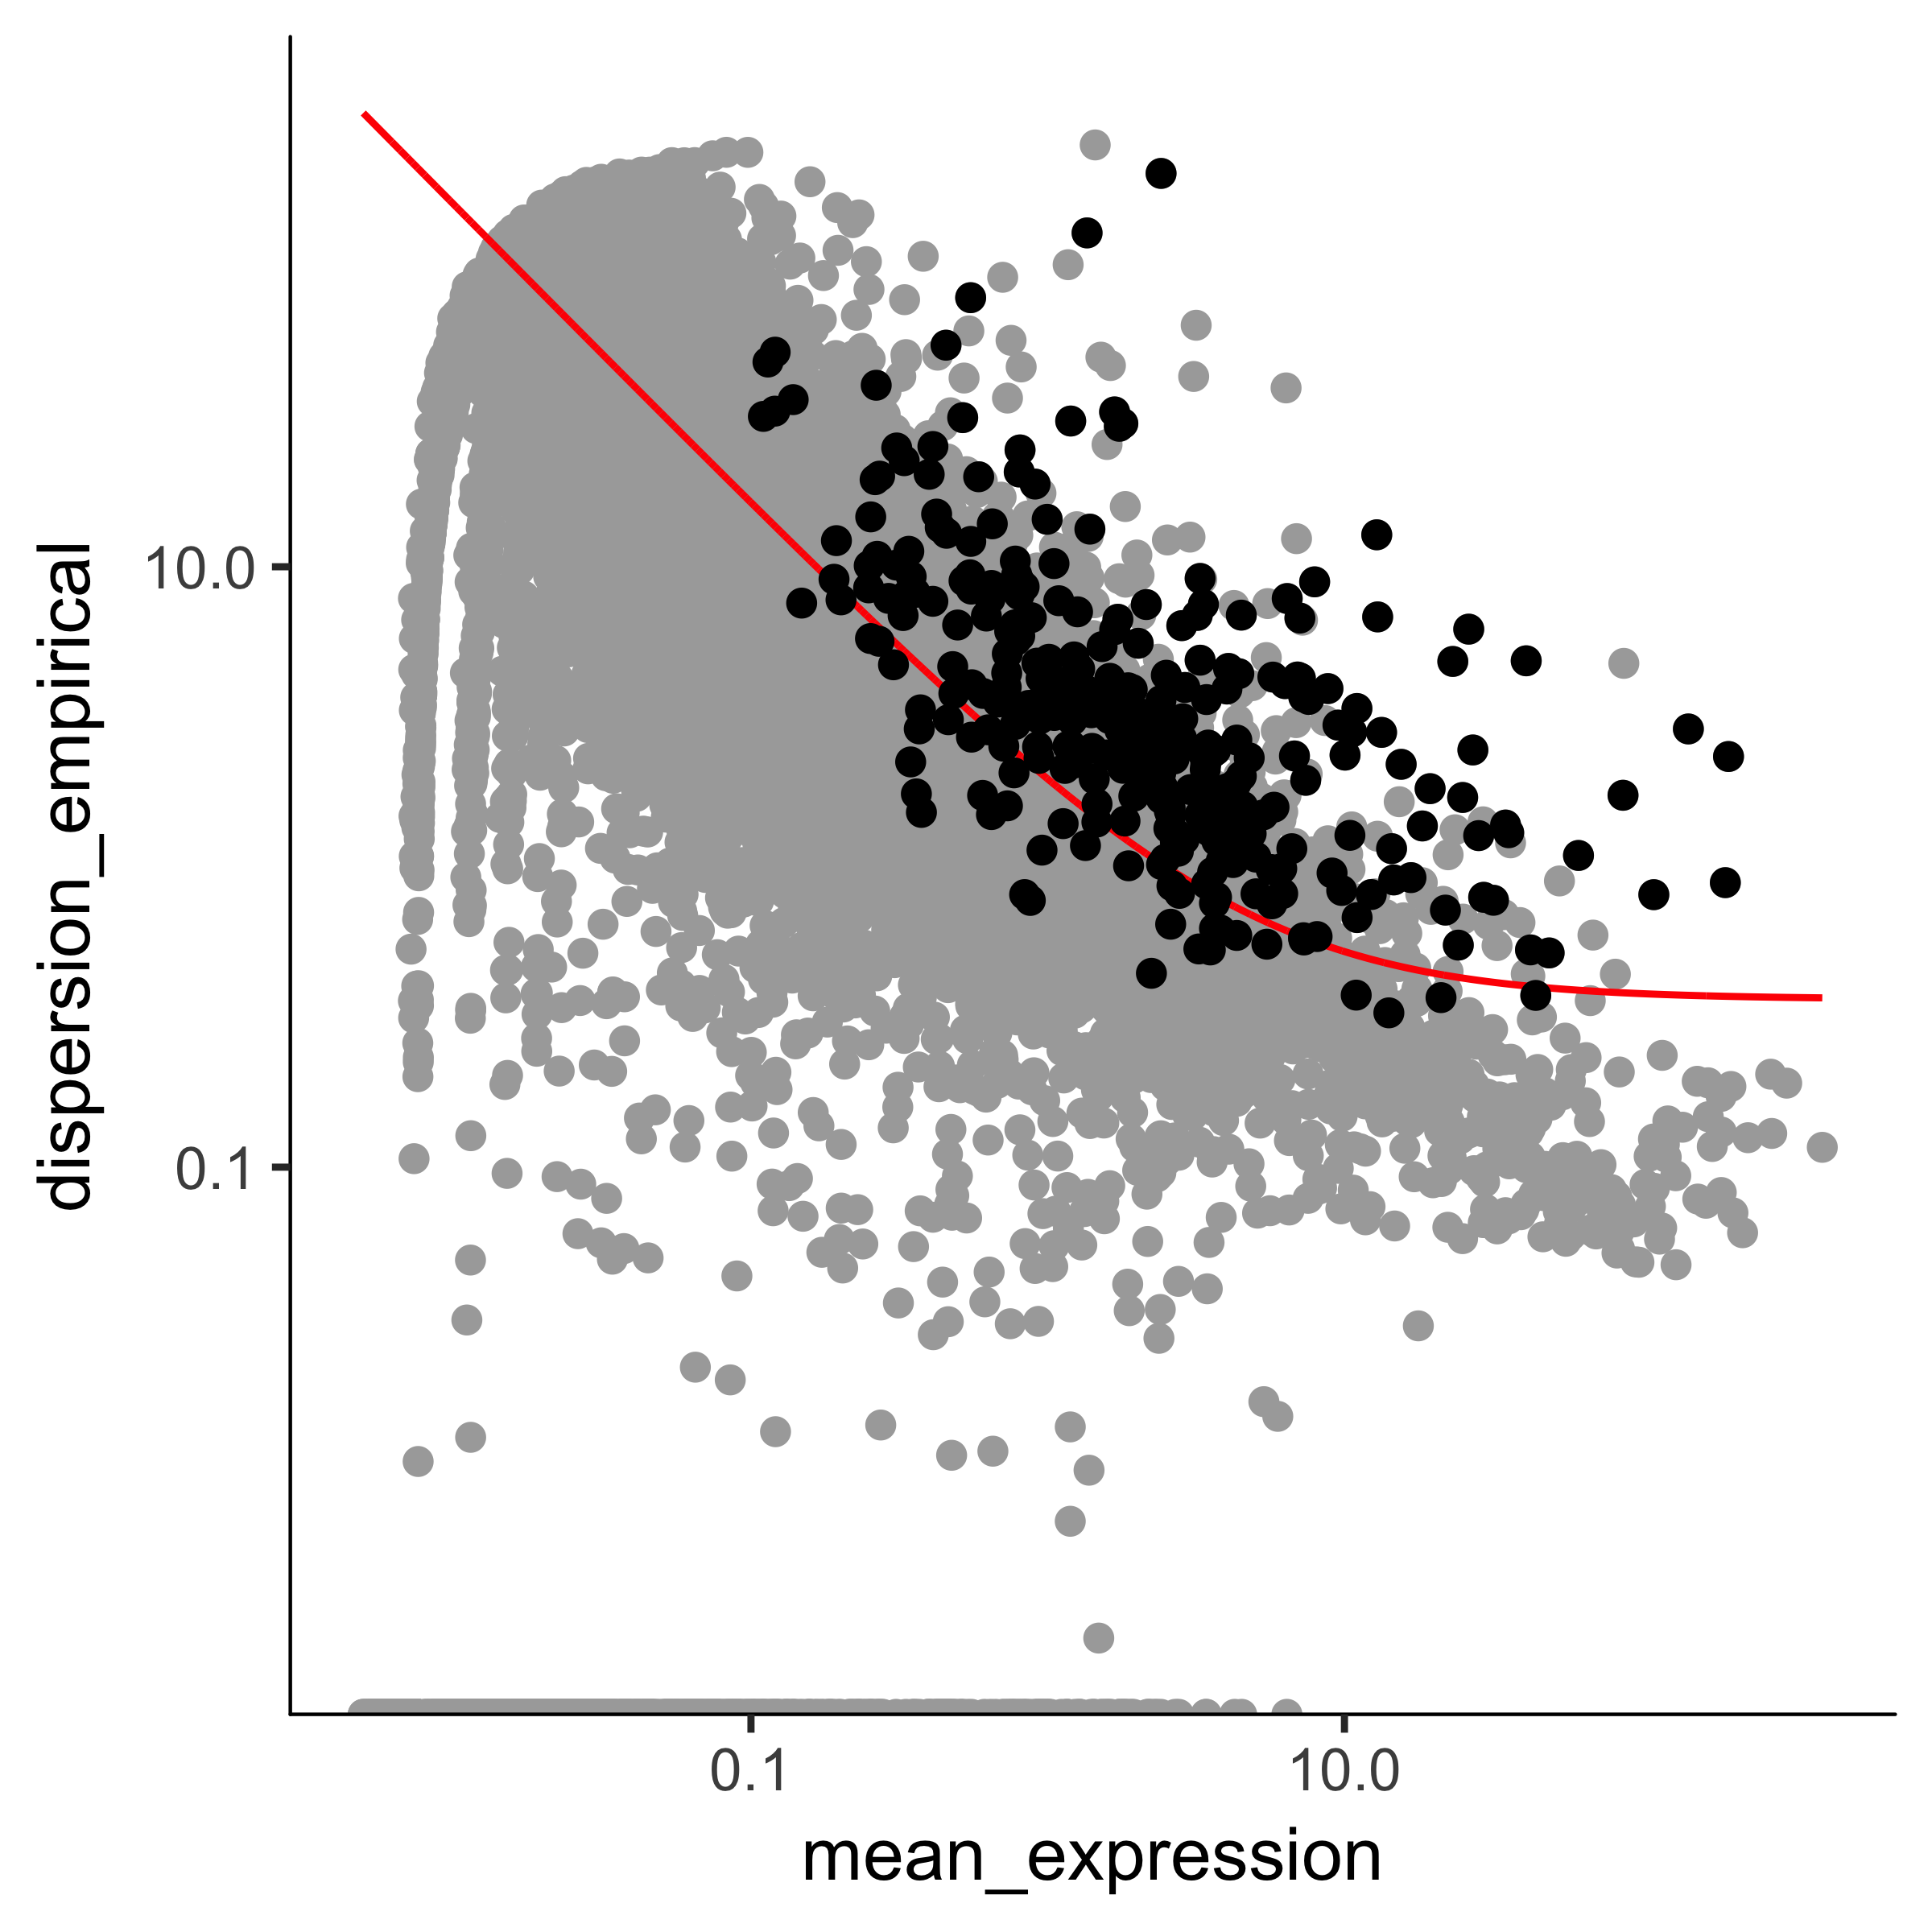
\includegraphics[width=\maxwidth]{figure/cluster_cells_semisup_pick_genes-1} 

}



\end{knitrout}

Note that we've got smaller set of genes, and some of them are not especially highly expressed or variable across the experiment. However, they are great for distinguishing cells that express \emph{MYF5} from those that have \emph{ANPEP}. We've already marked them for use in clustering, but even if we hadn't, we could still use them by providing them directly to \Rfunction{clusterCells}.

\begin{knitrout}
\definecolor{shadecolor}{rgb}{0.969, 0.969, 0.969}\color{fgcolor}\begin{kframe}
\begin{alltt}
\hlkwd{plot_pc_variance_explained}\hlstd{(HSMM,} \hlkwc{return_all} \hlstd{= F)} \hlcom{# }
\end{alltt}
\end{kframe}

{\centering 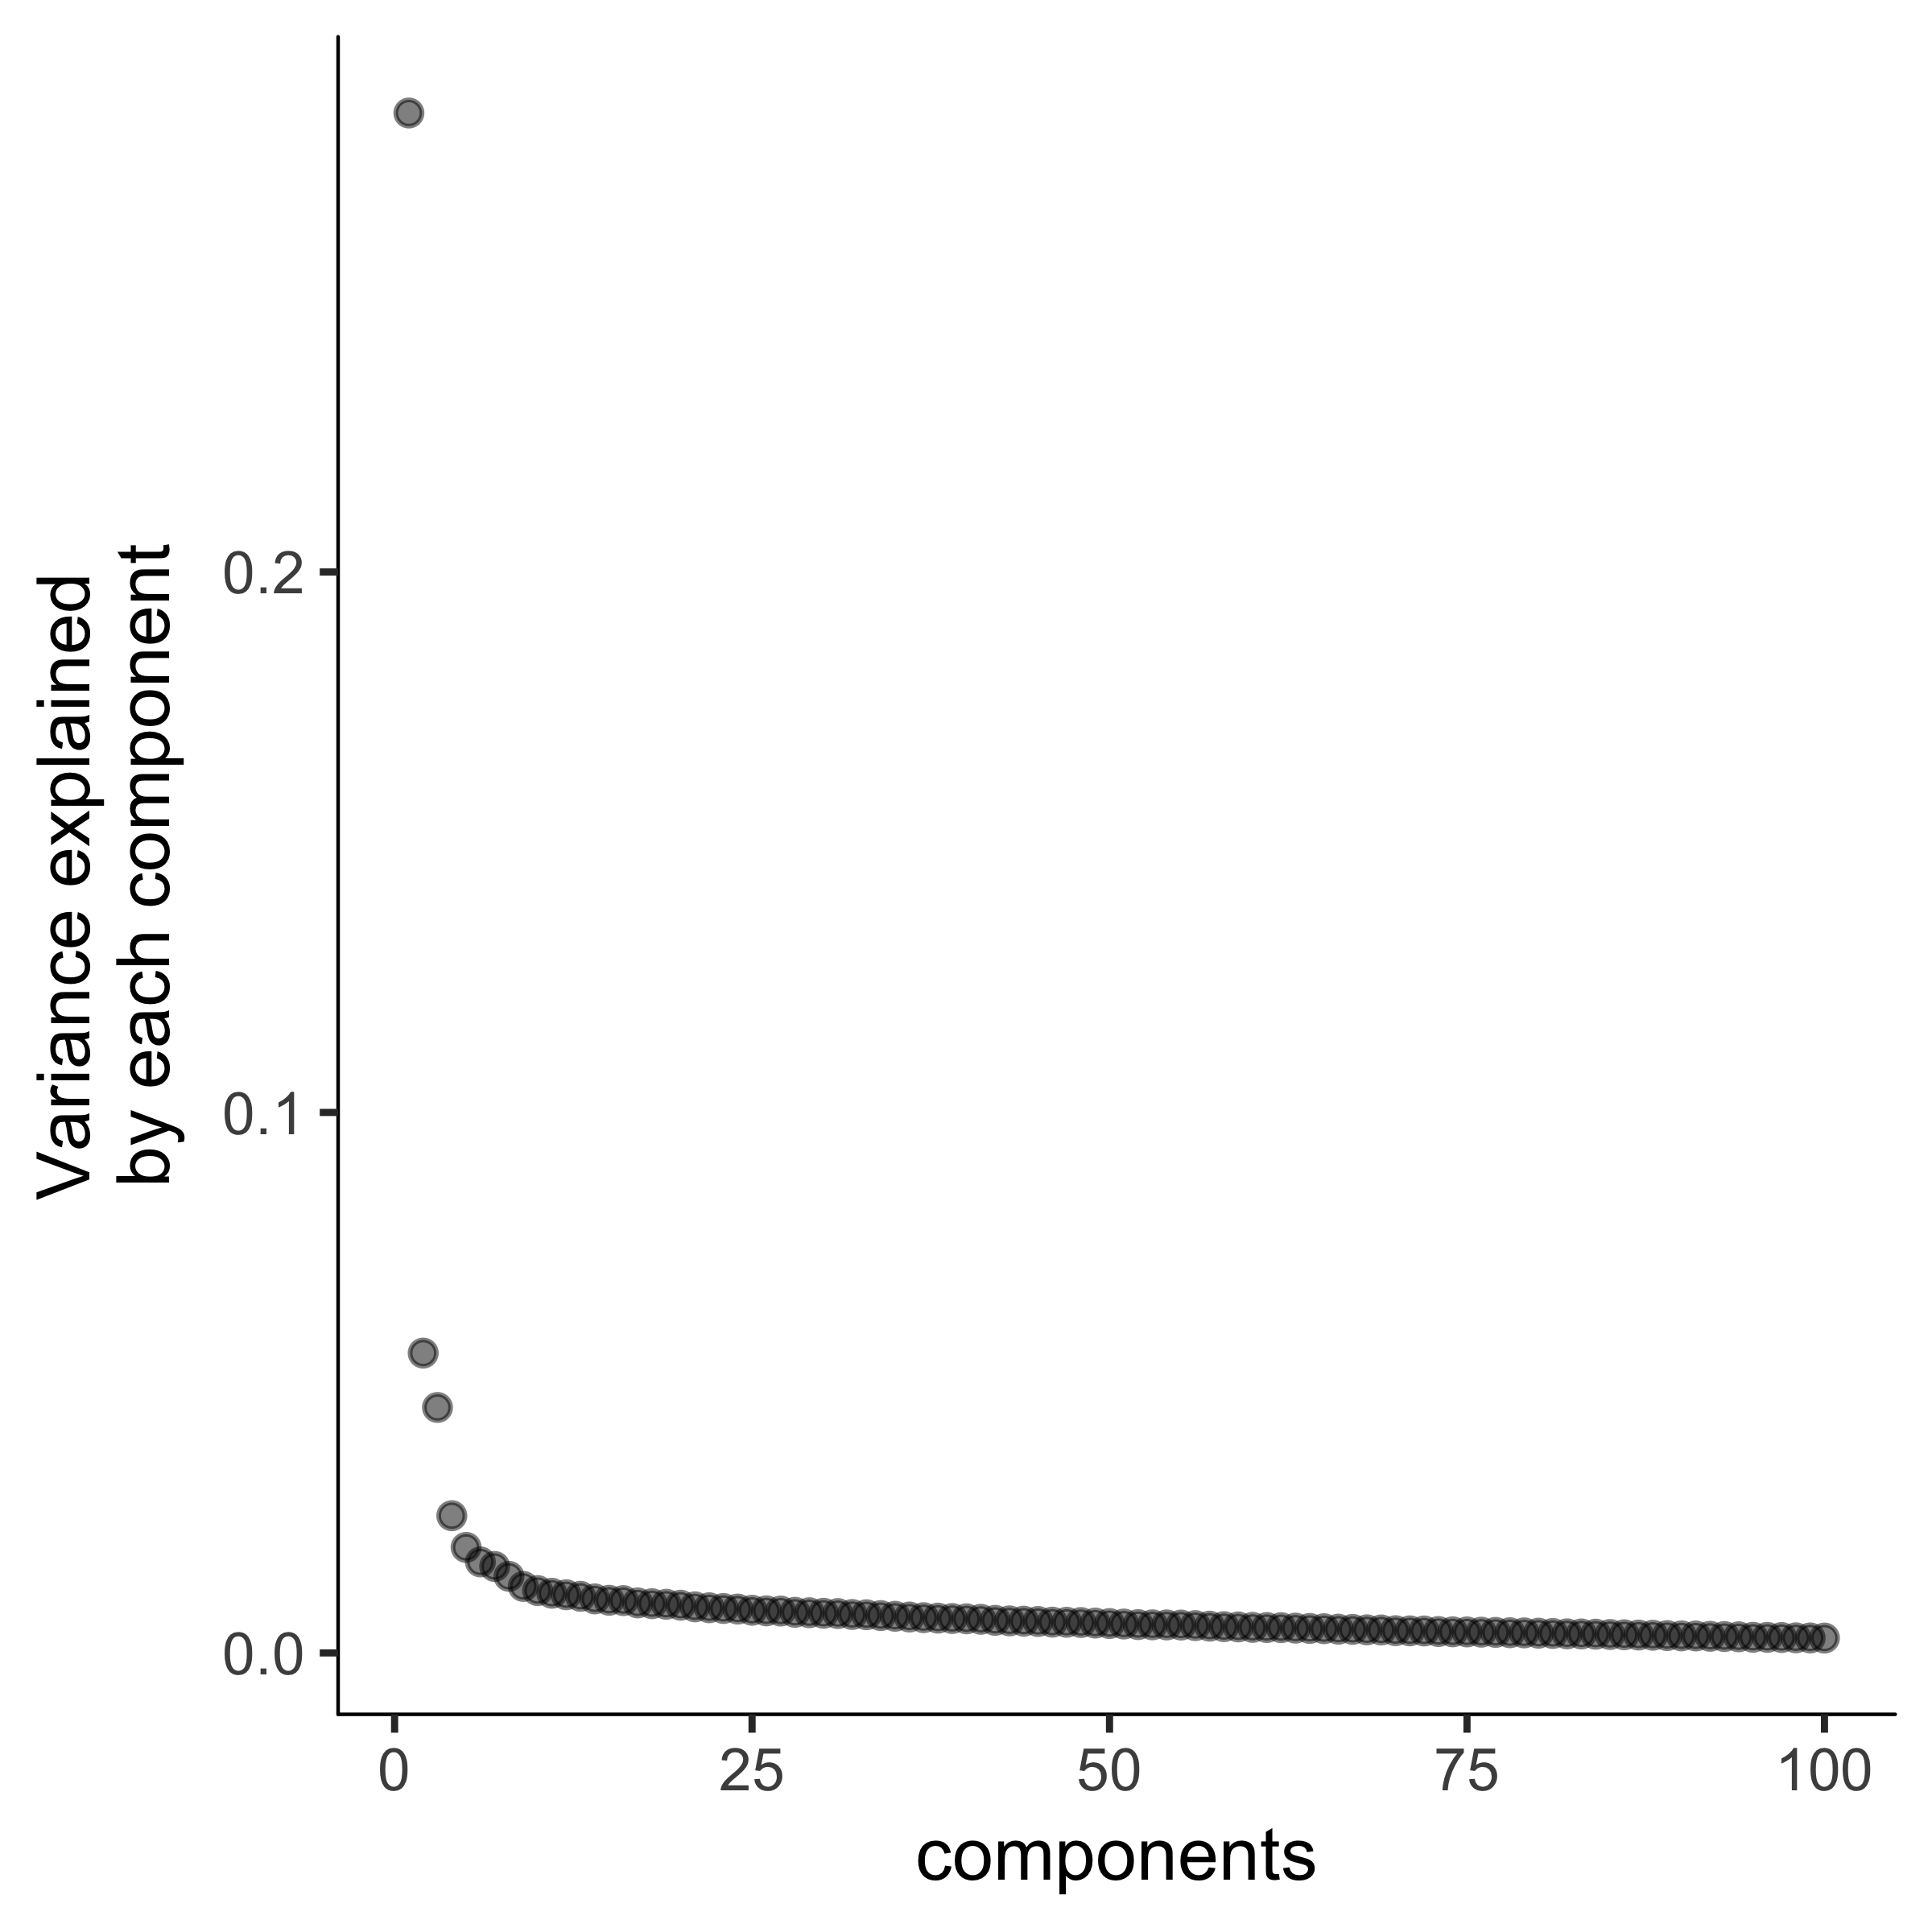
\includegraphics[width=\maxwidth]{figure/cluster_cells_semisup_clustering_no_impute-1} 

}


\begin{kframe}\begin{alltt}
\hlstd{HSMM} \hlkwb{<-} \hlkwd{reduceDimension}\hlstd{(HSMM,} \hlkwc{max_components}\hlstd{=}\hlnum{2}\hlstd{,} \hlkwc{num_dim} \hlstd{=} \hlnum{3}\hlstd{,} \hlkwc{norm_method} \hlstd{=} \hlstr{'log'}\hlstd{,} \hlkwc{reduction_method} \hlstd{=} \hlstr{'tSNE'}\hlstd{,}
                       \hlkwc{residualModelFormulaStr}\hlstd{=}\hlstr{"~Media + num_genes_expressed"}\hlstd{,} \hlkwc{verbose} \hlstd{= T)}
\end{alltt}


{\ttfamily\noindent\itshape\color{messagecolor}{\#\# Removing batch effects}}

{\ttfamily\noindent\itshape\color{messagecolor}{\#\# Remove noise by PCA ...}}

{\ttfamily\noindent\itshape\color{messagecolor}{\#\# Reduce dimension by tSNE ...}}\begin{alltt}
\hlstd{HSMM} \hlkwb{<-} \hlkwd{clusterCells}\hlstd{(HSMM,} \hlkwc{num_clusters}\hlstd{=}\hlnum{2}\hlstd{)}
\end{alltt}
\begin{verbatim}
## Distance cutoff calculated to 1.088545
\end{verbatim}


{\ttfamily\noindent\itshape\color{messagecolor}{\#\# the length of the distance: 34191}}\begin{alltt}
\hlkwd{plot_cell_clusters}\hlstd{(HSMM,} \hlnum{1}\hlstd{,} \hlnum{2}\hlstd{,} \hlkwc{color}\hlstd{=}\hlstr{"CellType"}\hlstd{)}
\end{alltt}
\end{kframe}

{\centering 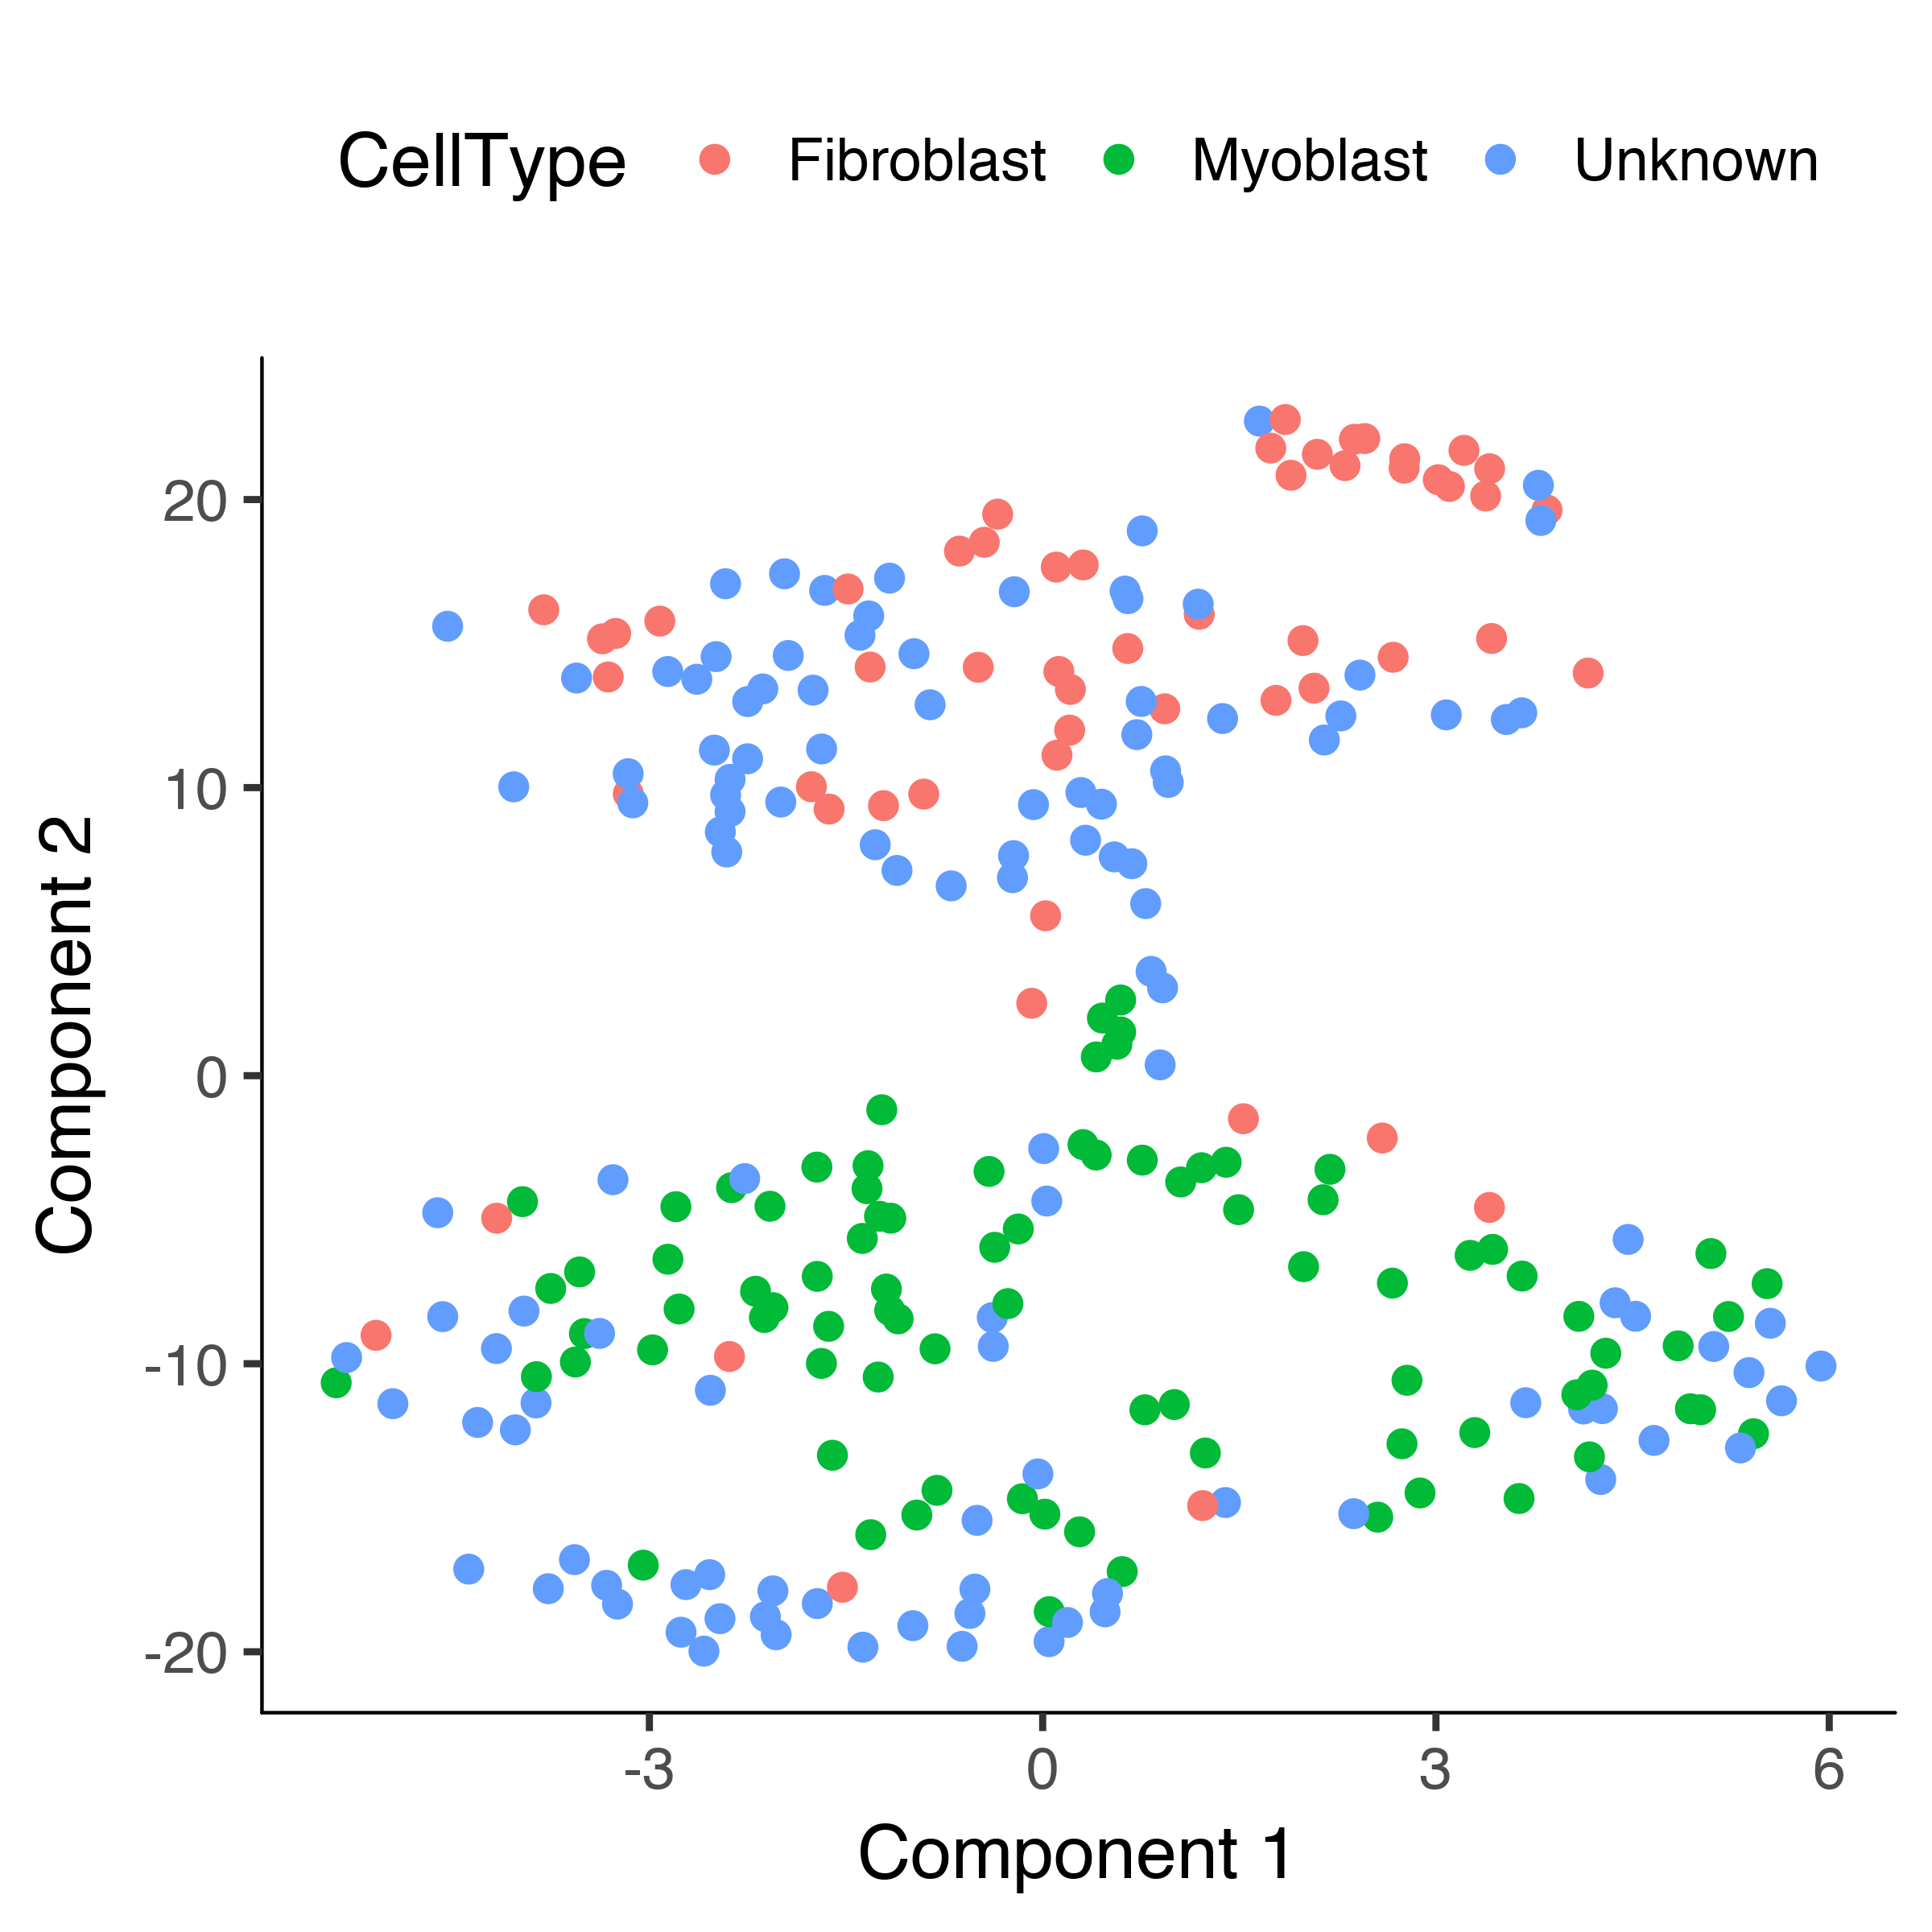
\includegraphics[width=\maxwidth]{figure/cluster_cells_semisup_clustering_no_impute-2} 

}



\end{knitrout}
 
 \subsection{Imputing cell type}
 
 Note that we've reduce the number of ``contaminating'' fibroblasts in the myoblast cluster, and vice versa. But what about the ``Unknown'' cells? If you provide \Rfunction{clusterCells} with a the CellTypeHierarcy, Monocle will use it classify \emph{whole clusters}, rather than just individual cells. Essentially, cluserCells works exactly as before, except after the clusters are built, it counts the frequency of each cell type in each cluster. When a cluster is composed of more than a certain percentage (in this case, 10\%) of a certain type, all the cells in the cluster are set to that type. If a cluster is composed of more than one cell type, the whole thing is marked ``Ambiguous''. If there's no cell type thats above the threshold, the cluster is marked ``Unknown''. Thus, Monocle helps you impute the type of each cell even in the presence of missing marker data.
 
\begin{knitrout}
\definecolor{shadecolor}{rgb}{0.969, 0.969, 0.969}\color{fgcolor}\begin{kframe}
\begin{alltt}
\hlstd{HSMM} \hlkwb{<-} \hlkwd{clusterCells}\hlstd{(HSMM,}
                     \hlkwc{num_clusters}\hlstd{=}\hlnum{2}\hlstd{,}
                     \hlkwc{frequency_thresh}\hlstd{=}\hlnum{0.1}\hlstd{,}
                     \hlkwc{cell_type_hierarchy}\hlstd{=cth)}
\end{alltt}
\begin{verbatim}
## Distance cutoff calculated to 1.088545
\end{verbatim}


{\ttfamily\noindent\itshape\color{messagecolor}{\#\# the length of the distance: 34191}}\begin{alltt}
\hlkwd{plot_cell_clusters}\hlstd{(HSMM,} \hlnum{1}\hlstd{,} \hlnum{2}\hlstd{,} \hlkwc{color}\hlstd{=}\hlstr{"CellType"}\hlstd{,} \hlkwc{markers} \hlstd{=} \hlkwd{c}\hlstd{(}\hlstr{"MYF5"}\hlstd{,} \hlstr{"ANPEP"}\hlstd{))}
\end{alltt}
\end{kframe}

{\centering 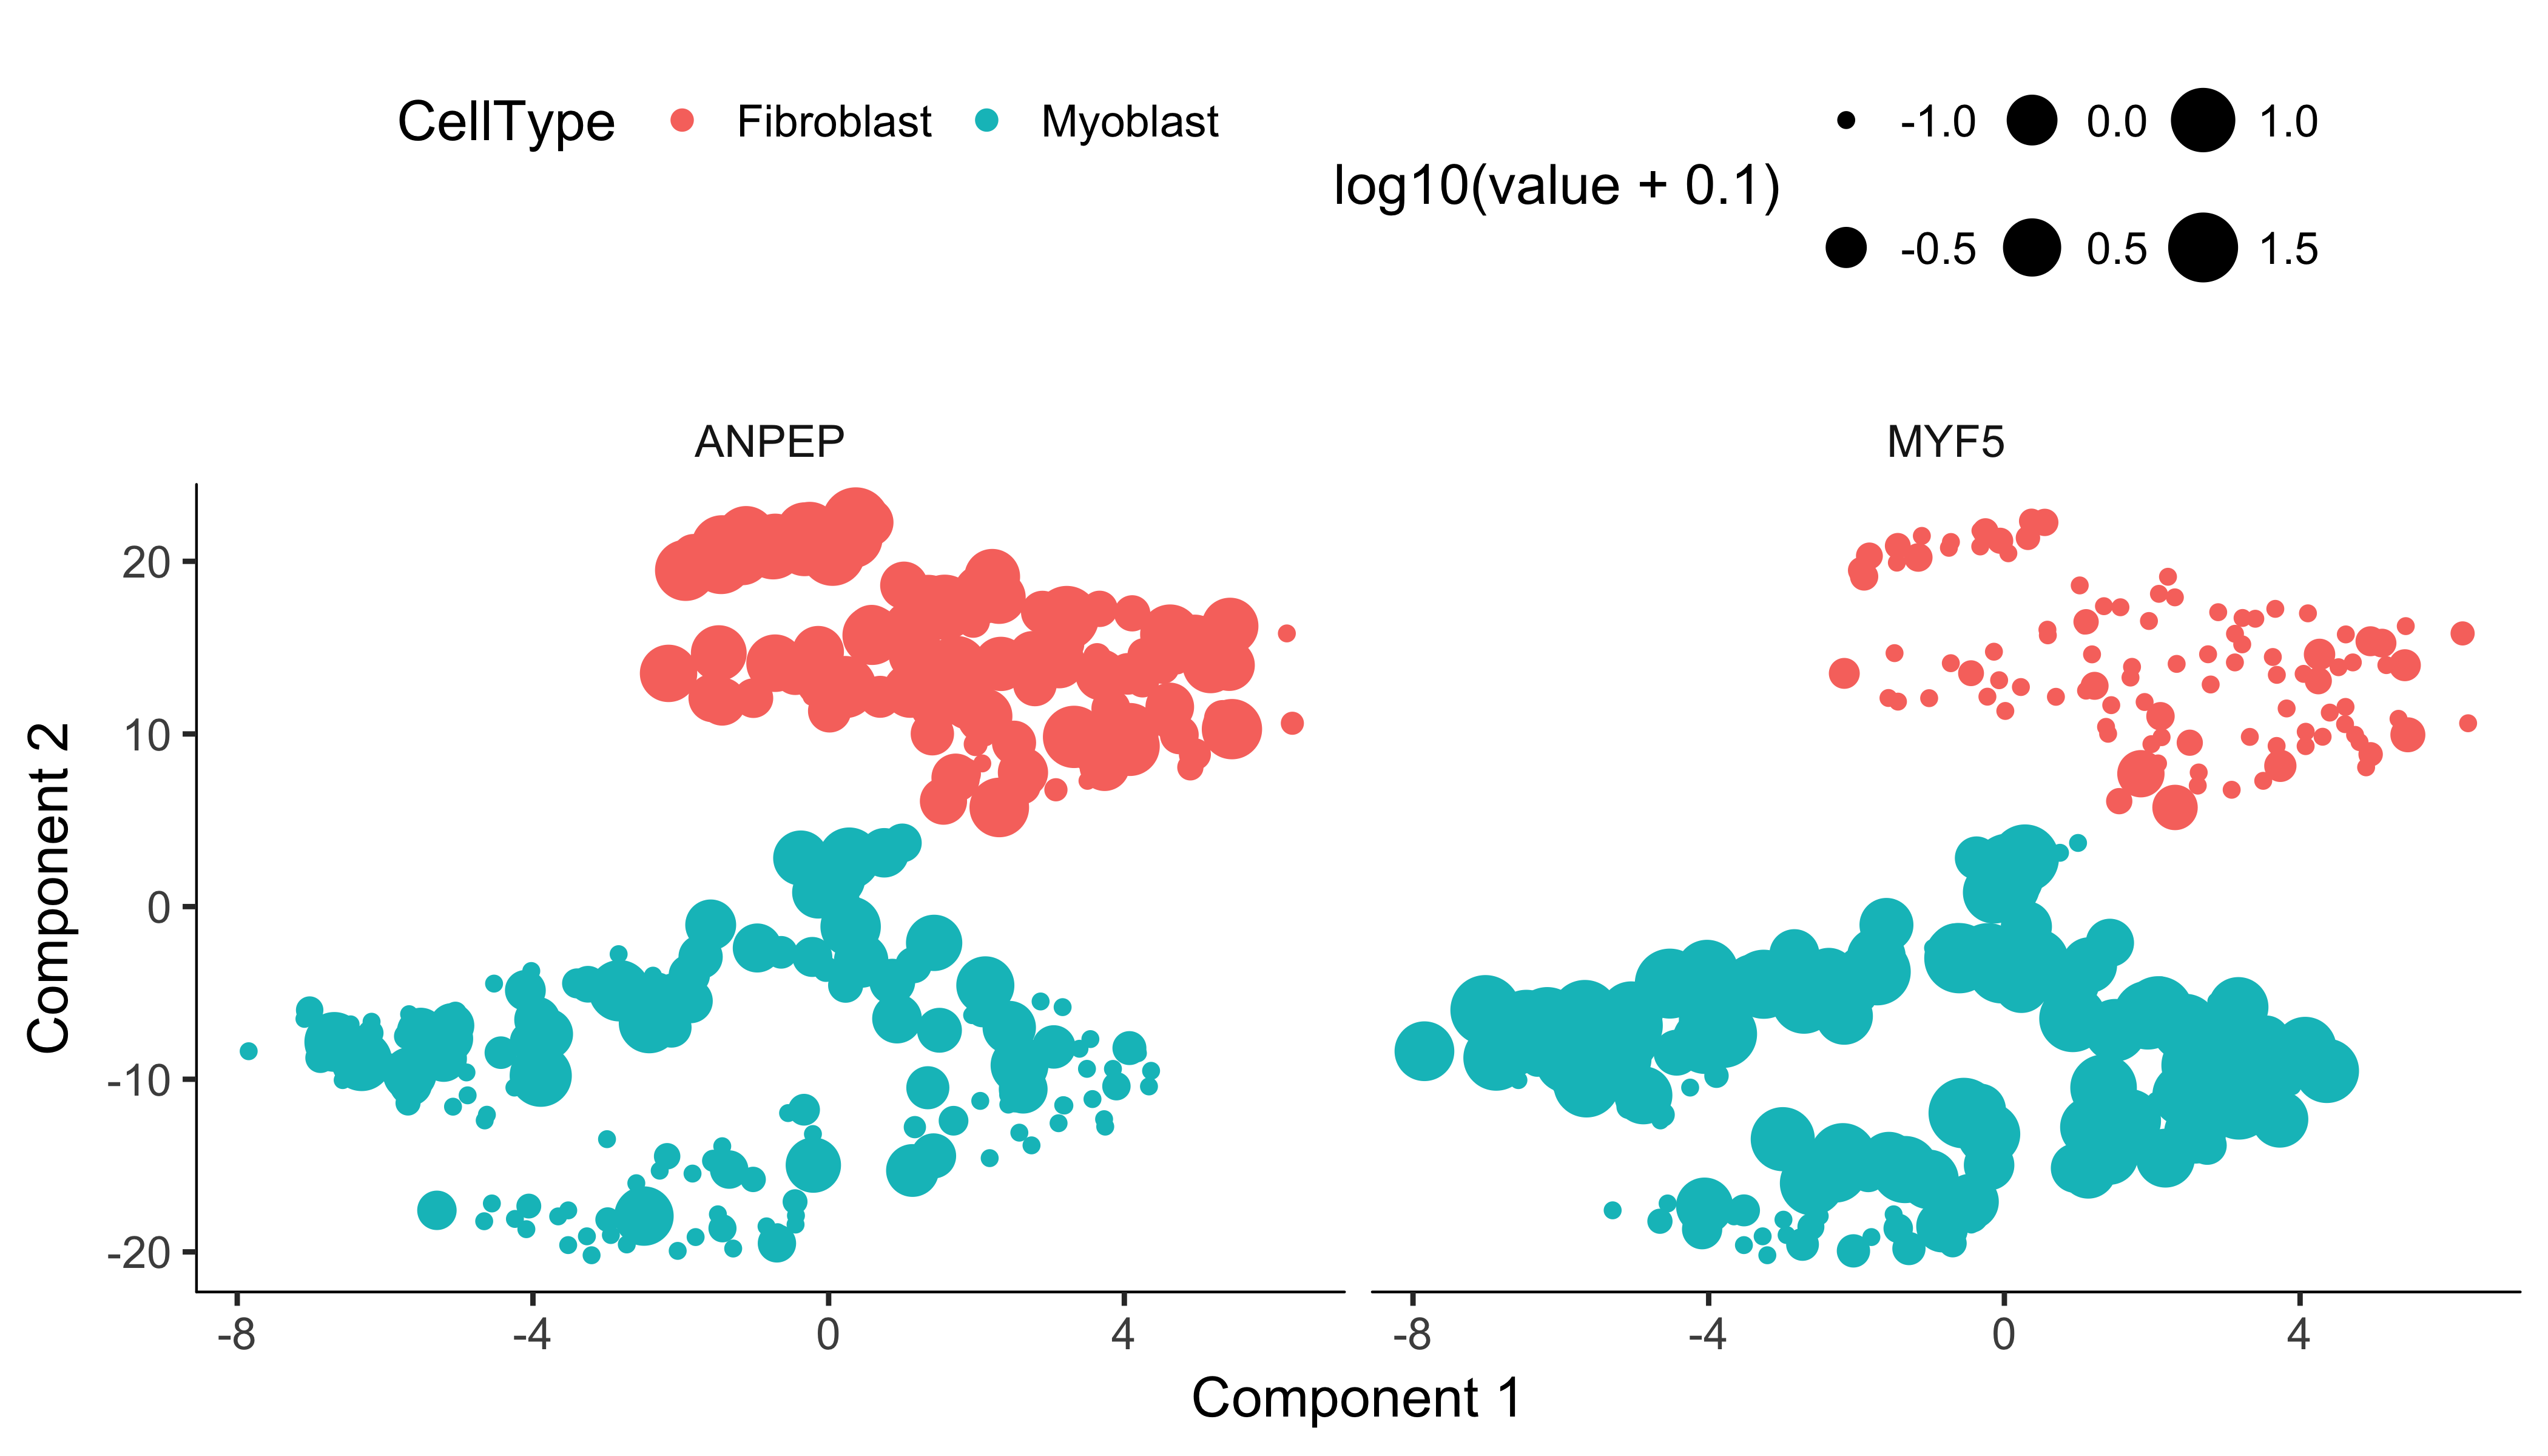
\includegraphics[width=\maxwidth]{figure/cluster_cells_semisup_clustering_with_impute-1} 

}



\end{knitrout}
 
As you can see, the clusters are fairly pure in terms of \emph{MYF5} expression. There are some cells expressing \emph{ANPEP} in both clusters, but those in the myoblast cluster also express \emph{MYF5}. This is not surprising, as ANPEP isn't a very specific marker of fibroblasts. Overall, we've successfully classified all the cells:
 
\begin{knitrout}
\definecolor{shadecolor}{rgb}{0.969, 0.969, 0.969}\color{fgcolor}\begin{kframe}
\begin{alltt}
\hlstd{pie} \hlkwb{<-} \hlkwd{ggplot}\hlstd{(}\hlkwd{pData}\hlstd{(HSMM),} \hlkwd{aes}\hlstd{(}\hlkwc{x} \hlstd{=} \hlkwd{factor}\hlstd{(}\hlnum{1}\hlstd{),} \hlkwc{fill} \hlstd{=} \hlkwd{factor}\hlstd{(CellType)))} \hlopt{+}
  \hlkwd{geom_bar}\hlstd{(}\hlkwc{width} \hlstd{=} \hlnum{1}\hlstd{)}
\hlstd{pie} \hlopt{+} \hlkwd{coord_polar}\hlstd{(}\hlkwc{theta} \hlstd{=} \hlstr{"y"}\hlstd{)} \hlopt{+}
  \hlkwd{theme}\hlstd{(}\hlkwc{axis.title.x}\hlstd{=}\hlkwd{element_blank}\hlstd{(),} \hlkwc{axis.title.y}\hlstd{=}\hlkwd{element_blank}\hlstd{())}
\end{alltt}
\end{kframe}

{\centering 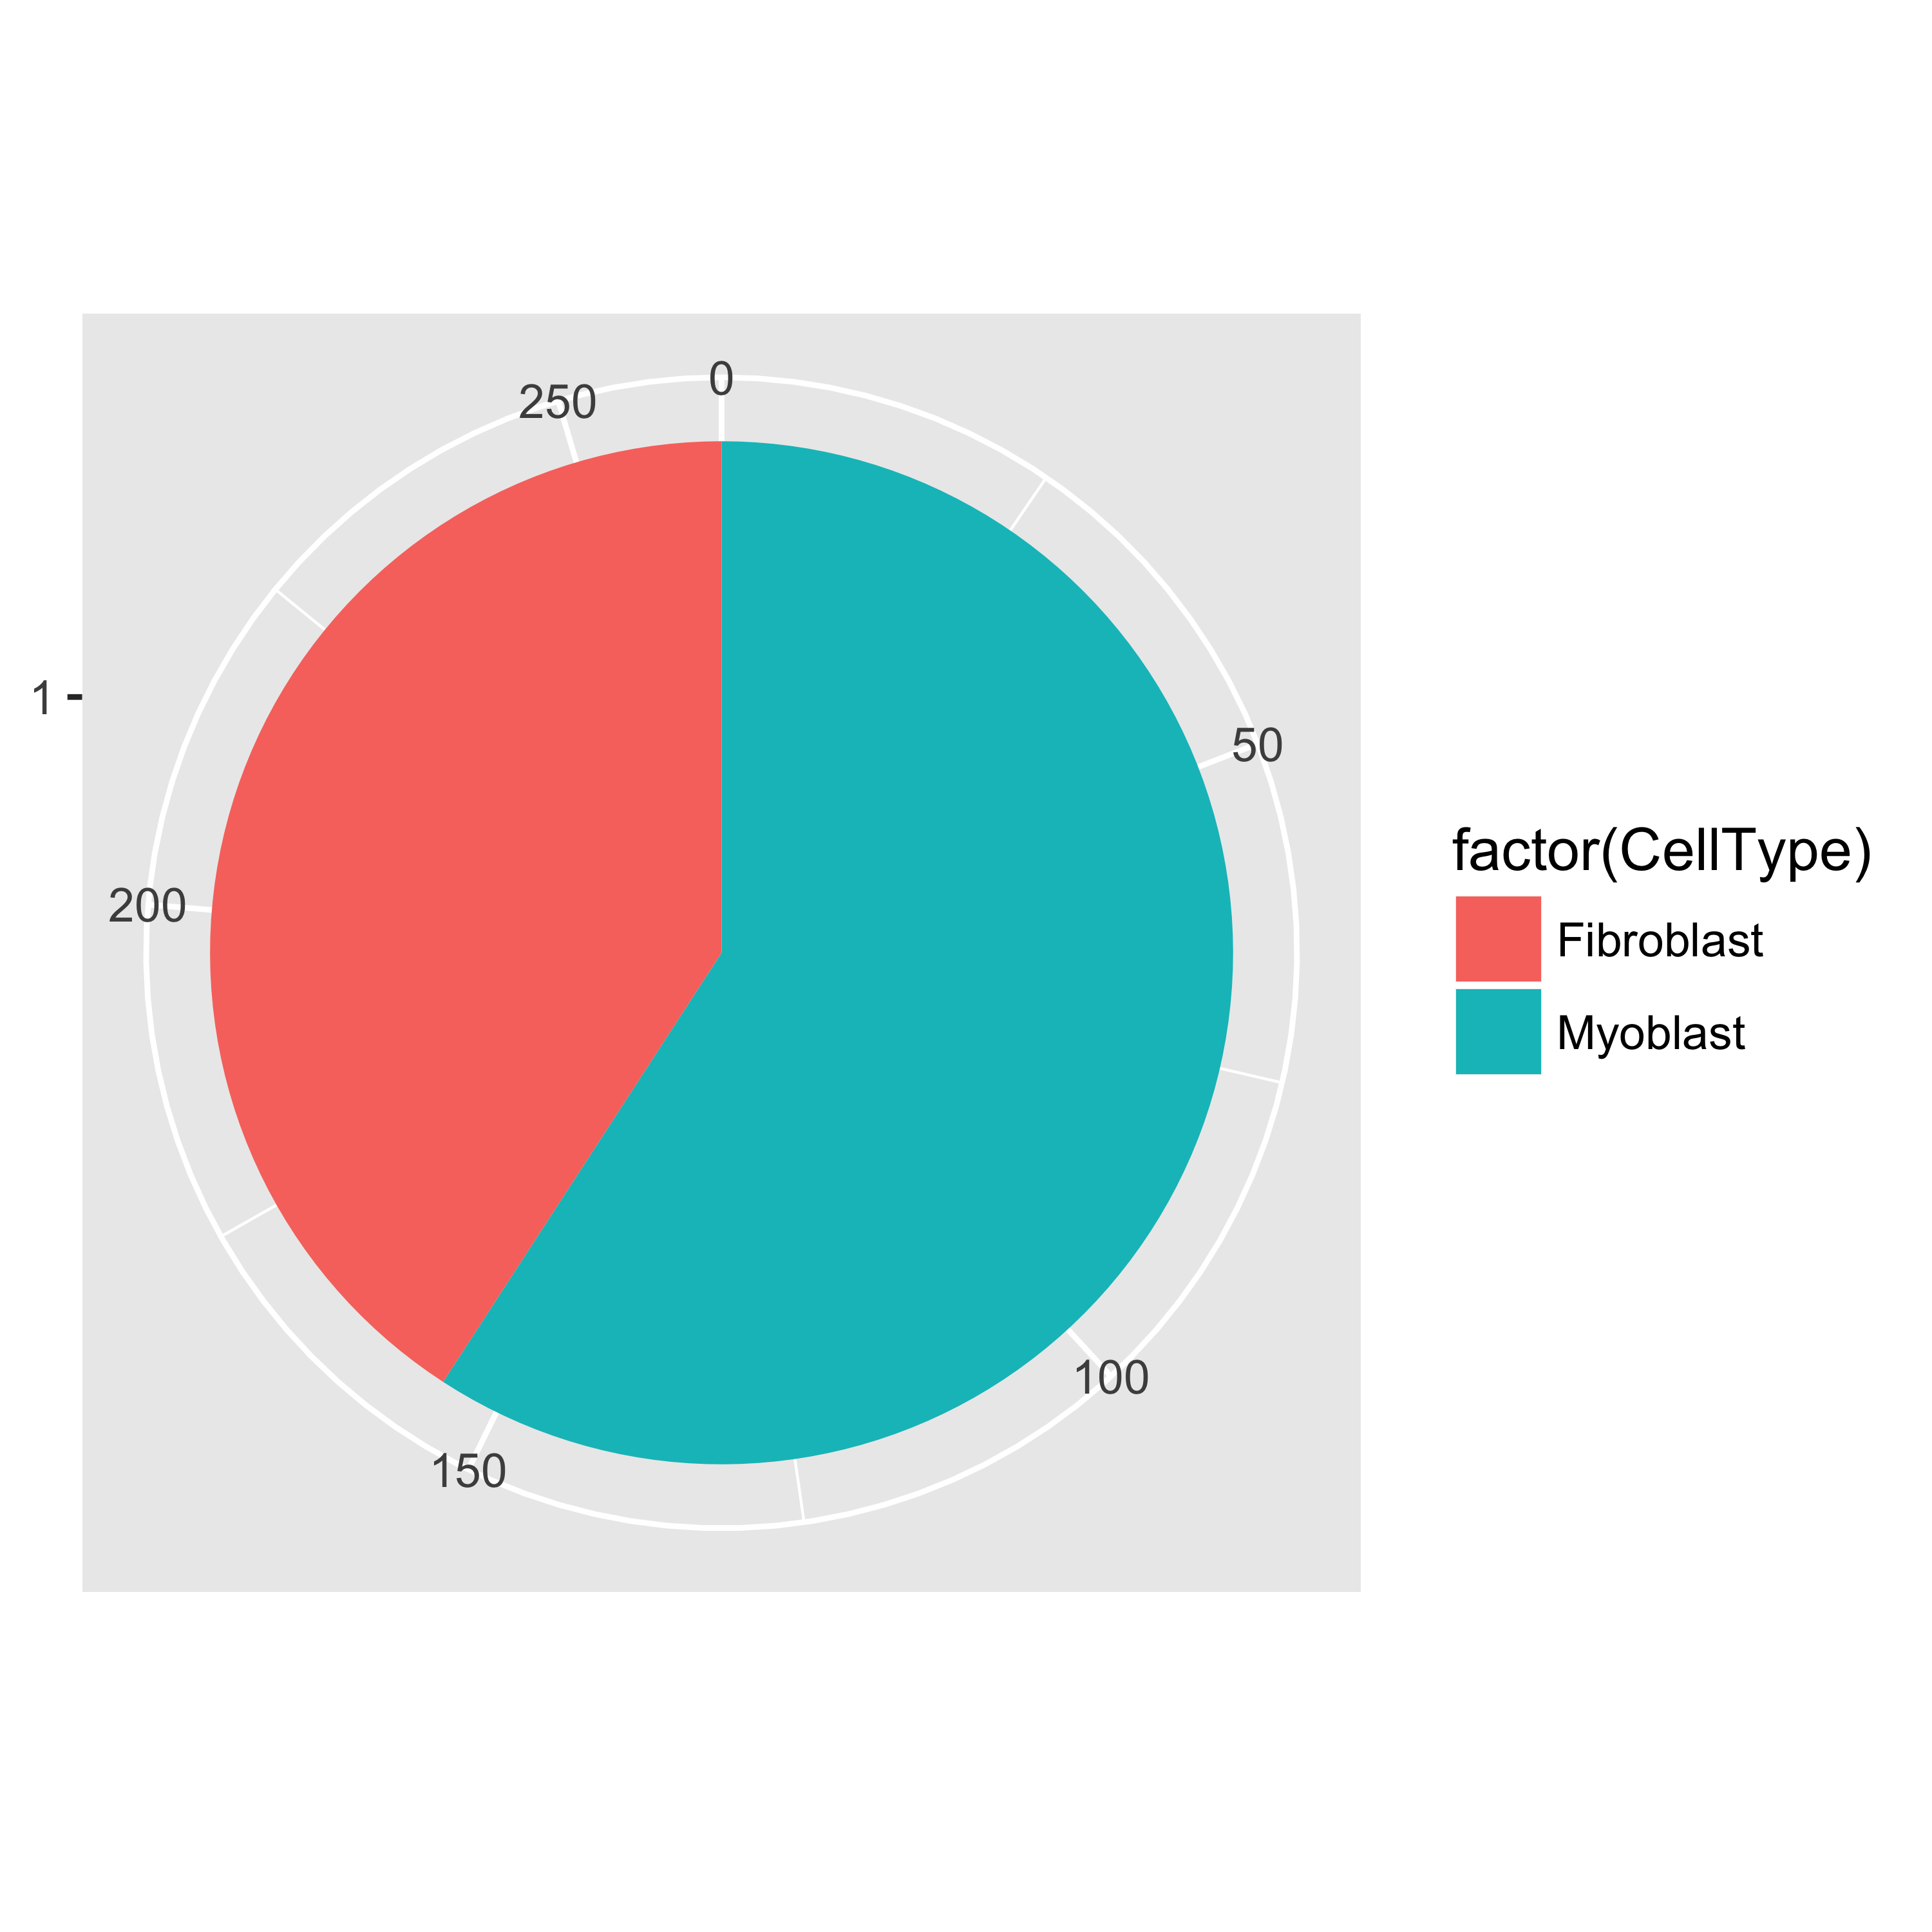
\includegraphics[width=\maxwidth]{figure/count_cells_semisup_pie-1} 

}



\end{knitrout}
 
 Finally, we subset the CellDataSet object to create \Robject{HSMM\_myo}, which includes only myoblasts. We'll use this in the rest of the analysis.
\begin{knitrout}
\definecolor{shadecolor}{rgb}{0.969, 0.969, 0.969}\color{fgcolor}\begin{kframe}
\begin{alltt}
\hlstd{HSMM_myo} \hlkwb{<-} \hlstd{HSMM[,}\hlkwd{pData}\hlstd{(HSMM)}\hlopt{$}\hlstd{CellType} \hlopt{==} \hlstr{"Myoblast"}\hlstd{]}
\hlstd{HSMM_myo} \hlkwb{<-} \hlkwd{estimateDispersions}\hlstd{(HSMM_myo)}
\end{alltt}


{\ttfamily\noindent\itshape\color{messagecolor}{\#\# Removing 127 outliers}}\end{kframe}
\end{knitrout}
 
 \section{Constructing single cell trajectories}
 
 During development, in response to stimuli, and througout life, cells transition from one functional ``state'' to another. Cells in different states express different sets of genes, producing a dynamic repetoire of proteins and metabolites that carry out their work. As cells move between states, undergo a process of transcriptional re-configuration, with some genes being silenced and others newly activated. These transient states are often hard to characterize because purifying cells in between more stable endpoint states can be difficult or impossible. Single-cell RNA-Seq can enable you to see these states without the need for purification. However, to do so, we must determine where each cell is the range of possible states. 
 
 Monocle introduced the strategy of using RNA-Seq for \emph{single cell trajectory analysis}. Rather than purifying cells into discrete states experimentally, Monocle uses an algorithm to learn the sequence of gene expression changes each cell must go through as part of a dynamic biological process. Once it has learned the overall ``trajectory'' of gene expression changes, Monocle can place each cell at its proper position in the trajectory. You can then use Monocle's differential analysis toolkit to find genes regulated over the course of the trajectory, as described in section \ref{pseudotime_diff}. If there are multiple outcome for the process, Monocle will reconstruct a ``branched'' trajectory. These branches correspond to cellular ``decisions'', and Monocle provides powerful tools for identifying the genes affected by them and involved in making them. You can see how to analyze branches in section \ref{BEAM}. Monocle relies on a machine learning technique called \emph{reversed graph embedding} to construct single-cell trajectories. You can read more about the theoretical foundations of Monocle's approach in section \ref{theory}, or consult the references shown below in section \ref{references}.
 
 \subsection{``Pseudotime'': a measure of progress through a biological process }
 
 In many biological processes, cells do not progress in perfect synchrony.  In single-cell expression studies of processes such as cell differentiation, captured cells might be widely distributed in terms of progress.  That is, in a population of cells captured at exactly the same time, some cells might be far along, while others might not yet even have begun the process.  This asynchrony creates major problems when you want to understand the sequence of regulatory changes that occur as cells transition from one state to the next. Tracking the expression across cells captured at the same time produces a very compressed sense of a gene's kinetics, and the apparent variability of that gene's expression will be very high. 
 
 By ordering each cell according to its progress along a learned trajectory, Monocle alleviates the problems that arise due to asynchrony. Instead of tracking changes in expression as a function of time, Monocle tracks changes as a function of progress along the trajectory, which we term ``pseudotime''. Pseudotime is an abstract unit of progress: it's simply the distance between a cell and the start of the trajectory, measured along the shortest path. The trajectory's total length is defined in terms of the total amount of transcriptional change that a cell undergoes as it moves from the starting state to the end state. For further details, see section \ref{theory}.
 
 \subsection{The ordering algorithm}
 
 \subsubsection{Choosing genes for ordering}
 Inferring a single-cell trajectory is a hard machine learning problem. The first step is to select the genes Monocle will use as input for its machine learning approach. This is called \emph{feature selection}, and it has a major impact in the shape of the trajectory. In single-cell RNA-Seq, genes expressed at low levels are often very noisy, but some may contain important information regarding the state of the cell.  If we simply provide all the input data, Monocle might get confused by the noise, or fix on a feature of the data that isn't biologically meaningful, such as batch effects arising from collecting data on different days. Monocle provides you with a variety of tools to select genes that will yield a robust, accurate, and biologically meaningful trajectory. You can use these tools to either perform a completely ``unsupervised'' analysis, in which Monocle has no forehand knowledge of which gene you consider important. Alternatively, you can make use of expert knowledge in the form of genes that are already known to define biolgical progress to shape Monocle's trajectory. We consider this mode ``semi-supervised'', because Monocle will augment the markers you provide with other, related genes. Monocle then uses these genes to produce trajectories consistent with known biology but that often reveal new regulatory structure. We return to the muscle data to illustrate both of these modes.
 
 \subsubsection{Reducing the dimensionality of the data}
 Once we have selected the genes we will use to order the cells, Monocle applies a \emph{dimensionality reduction} to the data, which will drastically improves the quality of the trajectory. Monocle reduces the dimensionality of the data with the \Rfunction{reduceDimension} function. This function has a number of options, so you should familiarize yourself with them by consulting the its manual page. You can choose from two algorithms in \Rfunction{reduceDimension}. The first, termed Independent Component Analysis, is a classic linear technique for decomposing data that powered the original version of Monocle. The second, called DDRTree, is a much more powerful nonlinear technique that is the default for Monocle 2.  For more on how these both work, see section \ref{theory}.   
 
 \subsubsection{Ordering the cells in pseudotime}
 With the expression data projected into a lower dimensional space, Monocle is ready to learn the trajectory that describes how cells transition from one state into another. Monocle assumes that the trajectory has a tree structure, with one end of it the ``root'', and the others the ``leaves''. A cell at the beginning of the biological process starts at the root and progresses along the trunk until it reaches the first branch, if there is one. It then chooses a branch, and moves further and further along the tree until it reaches a leaf. These mathematical assumptions translate into some important biological ones. First, that the data includes all the major stages of the biological process. If your experiment failed to capture any cells at a key developmental transition, Monocle won't know its there. Second, that gene expression changes are smooth as a cell moves from one stage to the next. This assumption is realistic: major discontinuities in the trajectory would amount to a cell almost instantaneously turning over its transcriptome, which probably doesn't happen in most biolgical processes.
 
 To order your cells, Monocle uses the \Rfunction{orderCells} function. This routine has one important argument, which allows you to set the root of the tree, and thus the beginning of the process. See the manual page for \Rfunction{orderCells} for more details.
 
 \subsection{Unsupervised ordering}
 
 In this section, we discuss ordering cells in a completely unsupervised fashion. First, we must decide which genes we will use to define a cell's progress through myogenesis. Monocle orders cells by examining the pattern of expression of these genes across the cell population. Monocle looks for genes that vary in ``interesting'' (i.e. not just noisy) ways, and uses these to structure the data. We ultimately want a set of genes that increase (or decrease) in expression as a function of progress through the process we're studying. 
 
 Ideally, we'd like to use as little prior knowledge of the biology of the system under study as possible. We'd like to discover the important ordering genes from the data, rather than relying on literature and textbooks, because that might introduce bias in the ordering. One effective way to isolate a set of ordering genes is to simply compare the cells collected at the beginning of the process to those at the end and find the differentially expressed genes, as described above. The command below will find all genes that are differentially expressed in response to the switch from growth medium to differentiation medium:
 
\begin{knitrout}
\definecolor{shadecolor}{rgb}{0.969, 0.969, 0.969}\color{fgcolor}\begin{kframe}
\begin{alltt}
\hlstd{diff_test_res} \hlkwb{<-} \hlkwd{differentialGeneTest}\hlstd{(HSMM_myo[expressed_genes,],}
                                      \hlkwc{fullModelFormulaStr}\hlstd{=}\hlstr{"~Media"}\hlstd{)}
\hlstd{ordering_genes} \hlkwb{<-} \hlkwd{row.names} \hlstd{(}\hlkwd{subset}\hlstd{(diff_test_res, qval} \hlopt{<} \hlnum{0.01}\hlstd{))}
\end{alltt}
\end{kframe}
\end{knitrout}
 
 Choosing genes based on differential analysis of time points is often highly effective, but what if we don't have time series data? If the cells are asynchronously moving through our biological process (as is usually the case), Monocle can often reconstruct their trajectory from a single population captured all at the same time. Below are two methods to select genes that require no knowledge of the design of the experiment at all.
 
\subsubsection{Selecting genes with high dispersion across cells} 
Genes that vary a lot are often highly informative for identifying cell subpopulations or ordering cells along a trajectory. In RNA-Seq, a gene's variance typically depends on its mean, so we have to be a bit careful about how we select genes based on their variance.
 
\begin{knitrout}
\definecolor{shadecolor}{rgb}{0.969, 0.969, 0.969}\color{fgcolor}\begin{kframe}
\begin{alltt}
\hlstd{disp_table} \hlkwb{<-} \hlkwd{dispersionTable}\hlstd{(HSMM_myo)}
\hlstd{ordering_genes} \hlkwb{<-} \hlkwd{subset}\hlstd{(disp_table,}
                         \hlstd{mean_expression} \hlopt{>=} \hlnum{0.5} \hlopt{&}
                         \hlstd{dispersion_empirical} \hlopt{>=} \hlnum{1} \hlopt{*} \hlstd{dispersion_fit)}\hlopt{$}\hlstd{gene_id}
\end{alltt}
\end{kframe}
\end{knitrout}
 
Once we have a list of gene ids to be used for ordering, we need to set them in the \Robject{HSMM} object, because the next several functions will depend on them.
 
\begin{knitrout}
\definecolor{shadecolor}{rgb}{0.969, 0.969, 0.969}\color{fgcolor}\begin{kframe}
\begin{alltt}
\hlstd{HSMM_myo} \hlkwb{<-} \hlkwd{setOrderingFilter}\hlstd{(HSMM_myo, ordering_genes)}
\hlkwd{plot_ordering_genes}\hlstd{(HSMM_myo)}
\end{alltt}
\end{kframe}

{\centering 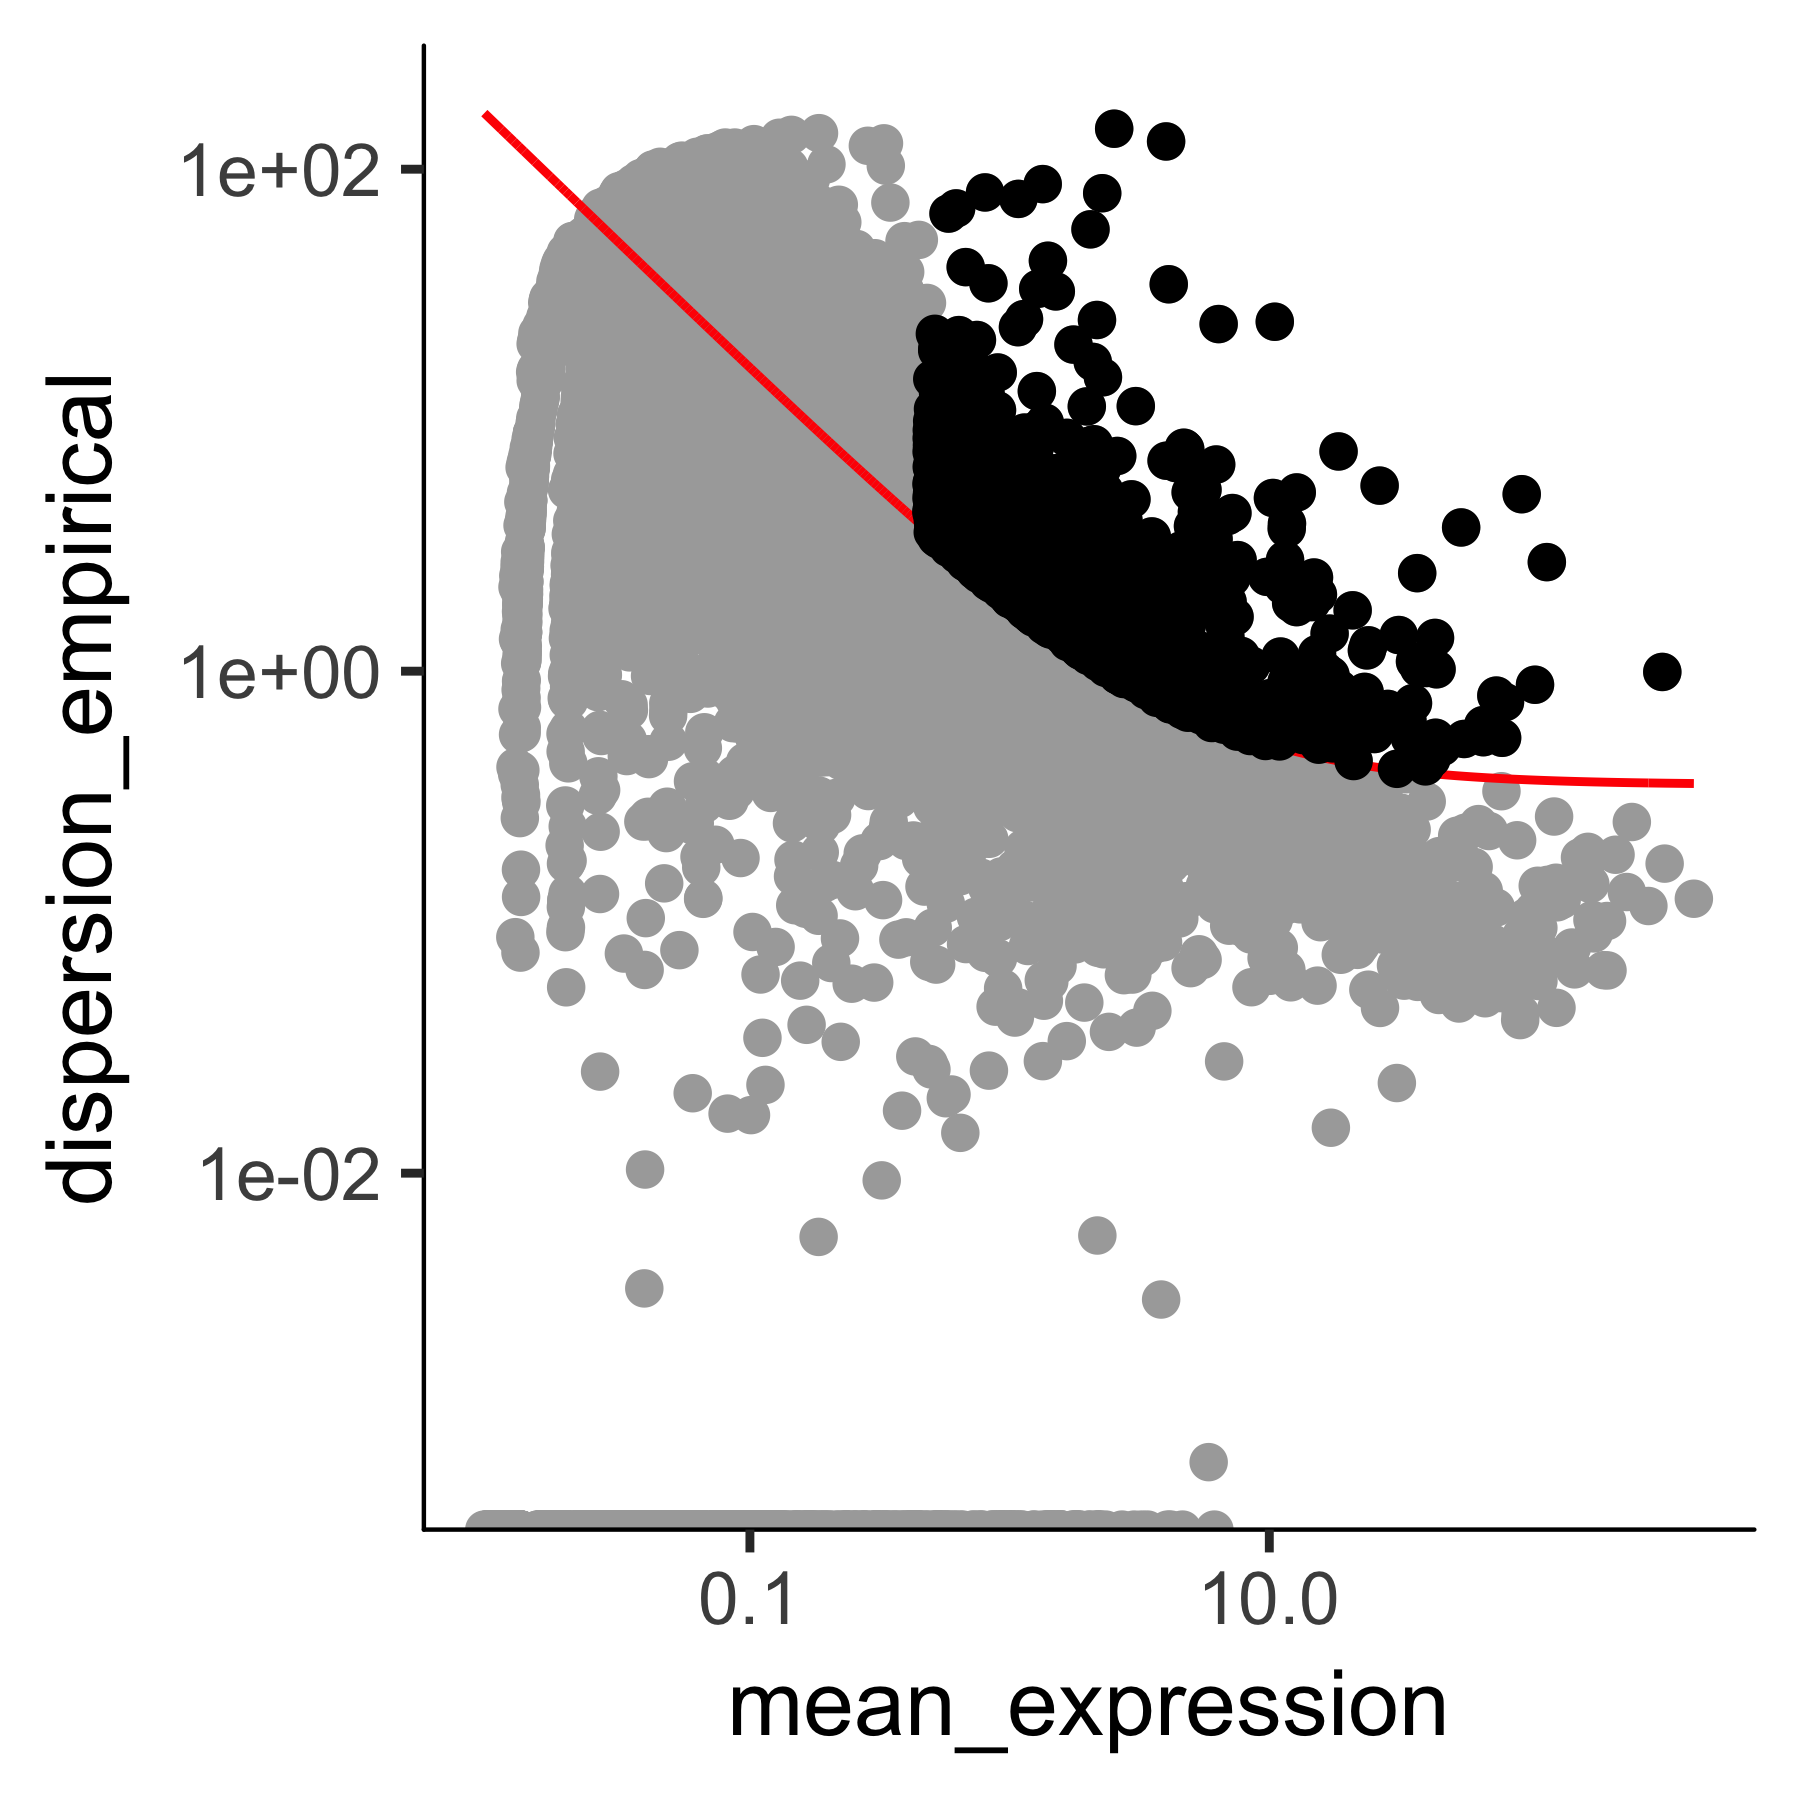
\includegraphics[width=\maxwidth]{figure/set_ordering_filter-1} 

}



\end{knitrout}
 
The genes we've chosen to use for ordering define the \emph{state space} of the cells in our data set.  Each cell is a point in this space, which has dimensionality equal to the number of genes we've chosen.  So if there are 500 genes used for ordering, each cell is a point in a 500-dimensional space.  For a number of reasons, Monocle works better if we can \emph{reduce} the dimensionality of that space before we try to put the cells in order.  In this case, we will reduce the space down to one with two dimensions, which we will be able to easily visualize and interpret while Monocle is ordering the cells.
\begin{knitrout}
\definecolor{shadecolor}{rgb}{0.969, 0.969, 0.969}\color{fgcolor}\begin{kframe}
\begin{alltt}
\hlstd{HSMM_myo} \hlkwb{<-} \hlkwd{reduceDimension}\hlstd{(HSMM_myo,} \hlkwc{max_components}\hlstd{=}\hlnum{2}\hlstd{,} \hlkwc{method} \hlstd{=} \hlstr{'DDRTree'}\hlstd{)}
\end{alltt}
\end{kframe}
\end{knitrout}
 
Now that the space is reduced, it's time to order the cells using the \Rfunction{orderCells} function as shown below. 

\begin{knitrout}
\definecolor{shadecolor}{rgb}{0.969, 0.969, 0.969}\color{fgcolor}\begin{kframe}
\begin{alltt}
\hlstd{HSMM_myo} \hlkwb{<-} \hlkwd{orderCells}\hlstd{(HSMM_myo)}
\end{alltt}
\end{kframe}
\end{knitrout}

Once the cells are ordered, we can visualize the trajectory in the reduced 
dimensional space.
 
\begin{knitrout}
\definecolor{shadecolor}{rgb}{0.969, 0.969, 0.969}\color{fgcolor}\begin{kframe}
\begin{alltt}
\hlkwd{plot_cell_trajectory}\hlstd{(HSMM_myo,} \hlkwc{color_by}\hlstd{=}\hlstr{"Hours"}\hlstd{)}
\end{alltt}
\end{kframe}

{\centering 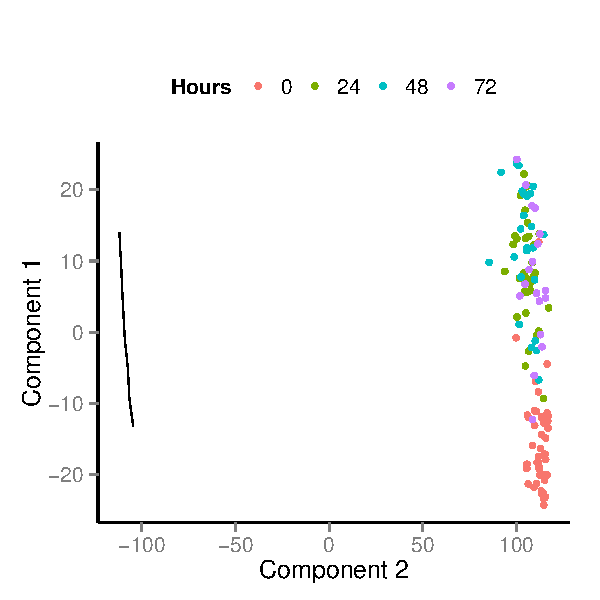
\includegraphics[width=\maxwidth]{figure/plot_ordering_mst-1} 

}



\end{knitrout}
 
% The second argument is the \Robject{reverse} flag.  Monocle won't be able to tell without some help which cells are at the beginning of the process and which are at the end.  The \Robject{reverse} flag tells Monocle to reverse the orientation of the entire process as it's being discovered from the data, so that the cells that would have been assigned to the end are instead assigned to the beginning, and so on. Setting \Robject{reverse} to true will reverse the ordering of the cells in pseudotime.   
 The trajectory has a tree-like structure. We can see that the cells 
 collected at time zero are located near one of the tips of the tree, while the 
 others are distributed amongst the two ``branches''.  Monocle doesn't know
 \emph{a priori} which of the trajectory of the tree to call the ``beginning'',
 so we often have to call \Rfunction{orderCells} again using the 
 \Robject{root\_state} argument to specify the beginning. First, we plot the
 trajectory, this time coloring the cells by ``State'':
 
\begin{knitrout}
\definecolor{shadecolor}{rgb}{0.969, 0.969, 0.969}\color{fgcolor}\begin{kframe}
\begin{alltt}
\hlkwd{plot_cell_trajectory}\hlstd{(HSMM_myo,} \hlkwc{color_by}\hlstd{=}\hlstr{"State"}\hlstd{)}
\end{alltt}
\end{kframe}

{\centering 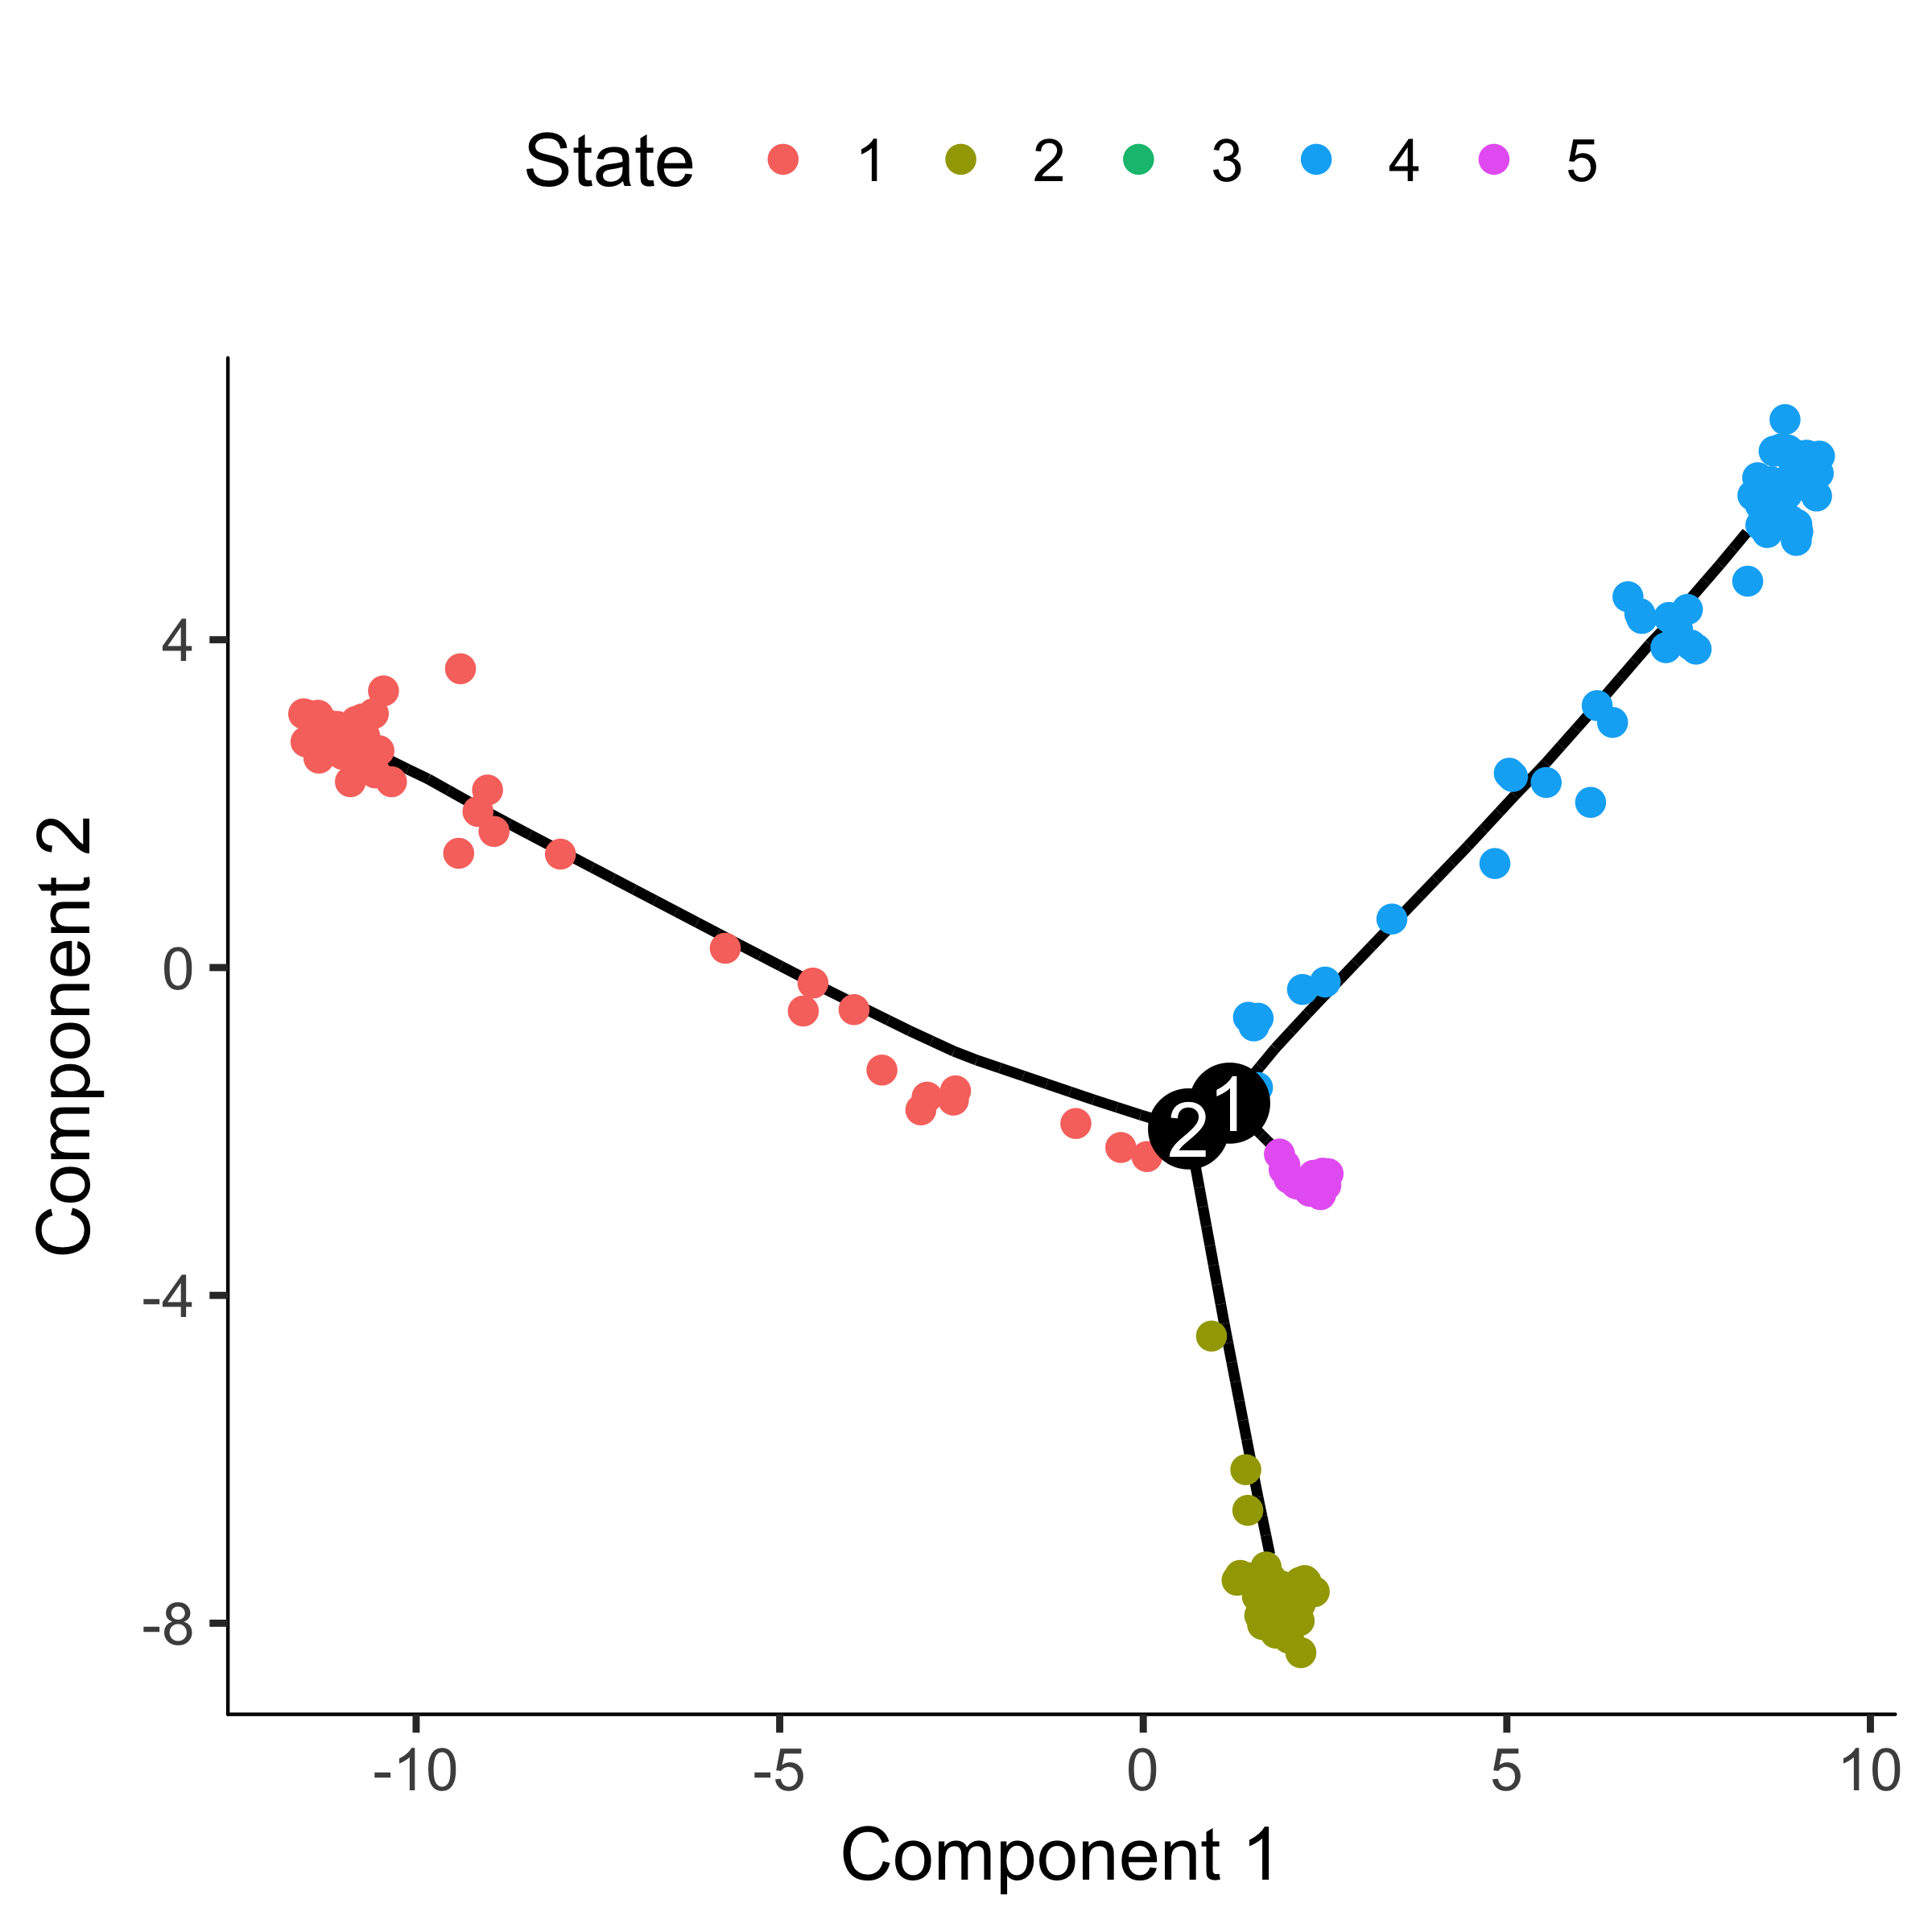
\includegraphics[width=\maxwidth]{figure/plot_ordering_mst_by_state-1} 

}



\end{knitrout}

``State'' is just Monocle's term for the segment of the tree. The function below is handy for identifying the State which contains most of the cells from time zero. We can then pass that to \Rfunction{orderCells}:

\begin{knitrout}
\definecolor{shadecolor}{rgb}{0.969, 0.969, 0.969}\color{fgcolor}\begin{kframe}
\begin{alltt}
\hlstd{GM_state} \hlkwb{<-} \hlkwa{function}\hlstd{(}\hlkwc{cds}\hlstd{)\{}
  \hlkwa{if} \hlstd{(}\hlkwd{length}\hlstd{(}\hlkwd{unique}\hlstd{(}\hlkwd{pData}\hlstd{(cds)}\hlopt{$}\hlstd{State))} \hlopt{>} \hlnum{1}\hlstd{)\{}
    \hlstd{T0_counts} \hlkwb{<-} \hlkwd{table}\hlstd{(}\hlkwd{pData}\hlstd{(cds)}\hlopt{$}\hlstd{State,} \hlkwd{pData}\hlstd{(cds)}\hlopt{$}\hlstd{Hours)[,}\hlstr{"0"}\hlstd{]}
    \hlkwd{return}\hlstd{(}\hlkwd{as.numeric}\hlstd{(}\hlkwd{names}\hlstd{(T0_counts)[}\hlkwd{which}\hlstd{(T0_counts} \hlopt{==} \hlkwd{max}\hlstd{(T0_counts))]))}
  \hlstd{\}}\hlkwa{else} \hlstd{\{} \hlkwd{return} \hlstd{(}\hlnum{1}\hlstd{) \}}
\hlstd{\}}
\hlstd{HSMM_myo} \hlkwb{<-} \hlkwd{orderCells}\hlstd{(HSMM_myo,} \hlkwc{root_state}\hlstd{=}\hlkwd{GM_state}\hlstd{(HSMM_myo))}
\hlkwd{plot_cell_trajectory}\hlstd{(HSMM_myo,} \hlkwc{color_by}\hlstd{=}\hlstr{"Pseudotime"}\hlstd{)}
\end{alltt}
\end{kframe}

{\centering 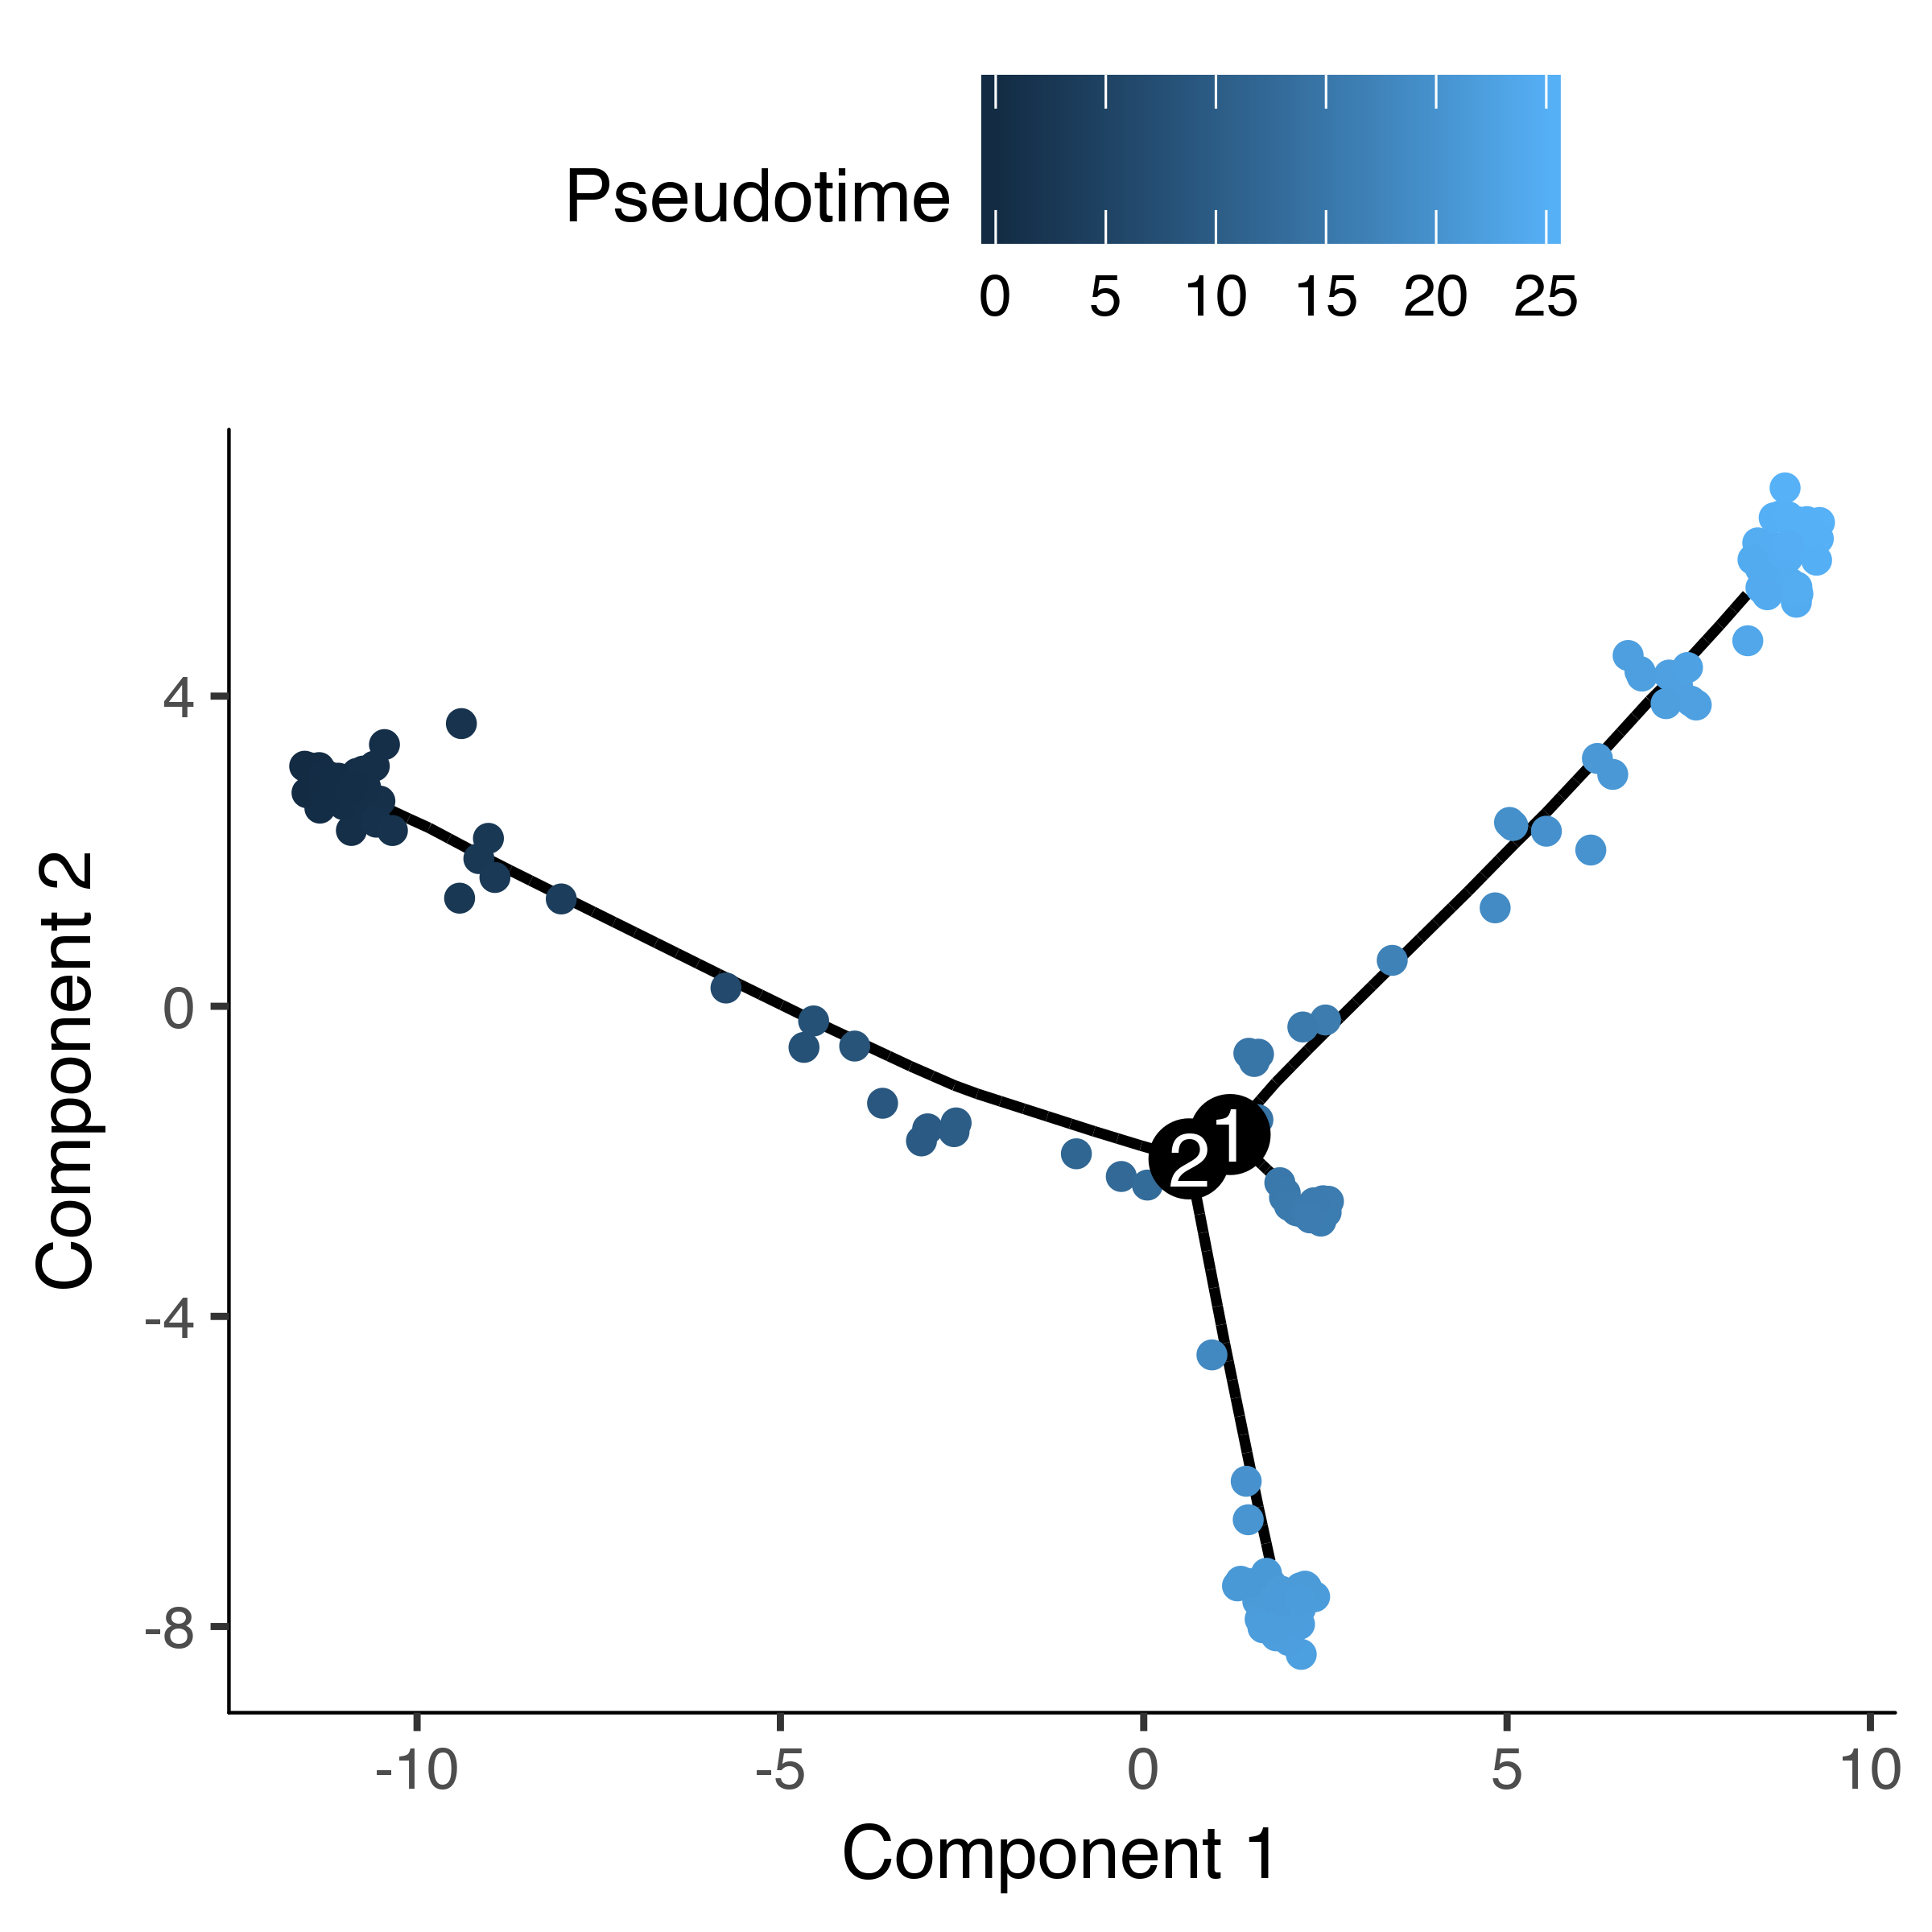
\includegraphics[width=\maxwidth]{figure/plot_ordering_with_GM_state-1} 

}



\end{knitrout}

If there are a ton of states in your tree, it can be a little hard to make out where each one falls on the tree.  Sometimes it can be handy to ``facet'' the trajectory plot so it's easier to see where each of the states are located:

\begin{knitrout}
\definecolor{shadecolor}{rgb}{0.969, 0.969, 0.969}\color{fgcolor}\begin{kframe}
\begin{alltt}
\hlkwd{plot_cell_trajectory}\hlstd{(HSMM_myo,} \hlkwc{color_by}\hlstd{=}\hlstr{"State"}\hlstd{)} \hlopt{+} \hlkwd{facet_wrap}\hlstd{(}\hlopt{~}\hlstd{State,} \hlkwc{nrow}\hlstd{=}\hlnum{1}\hlstd{)}
\end{alltt}
\end{kframe}
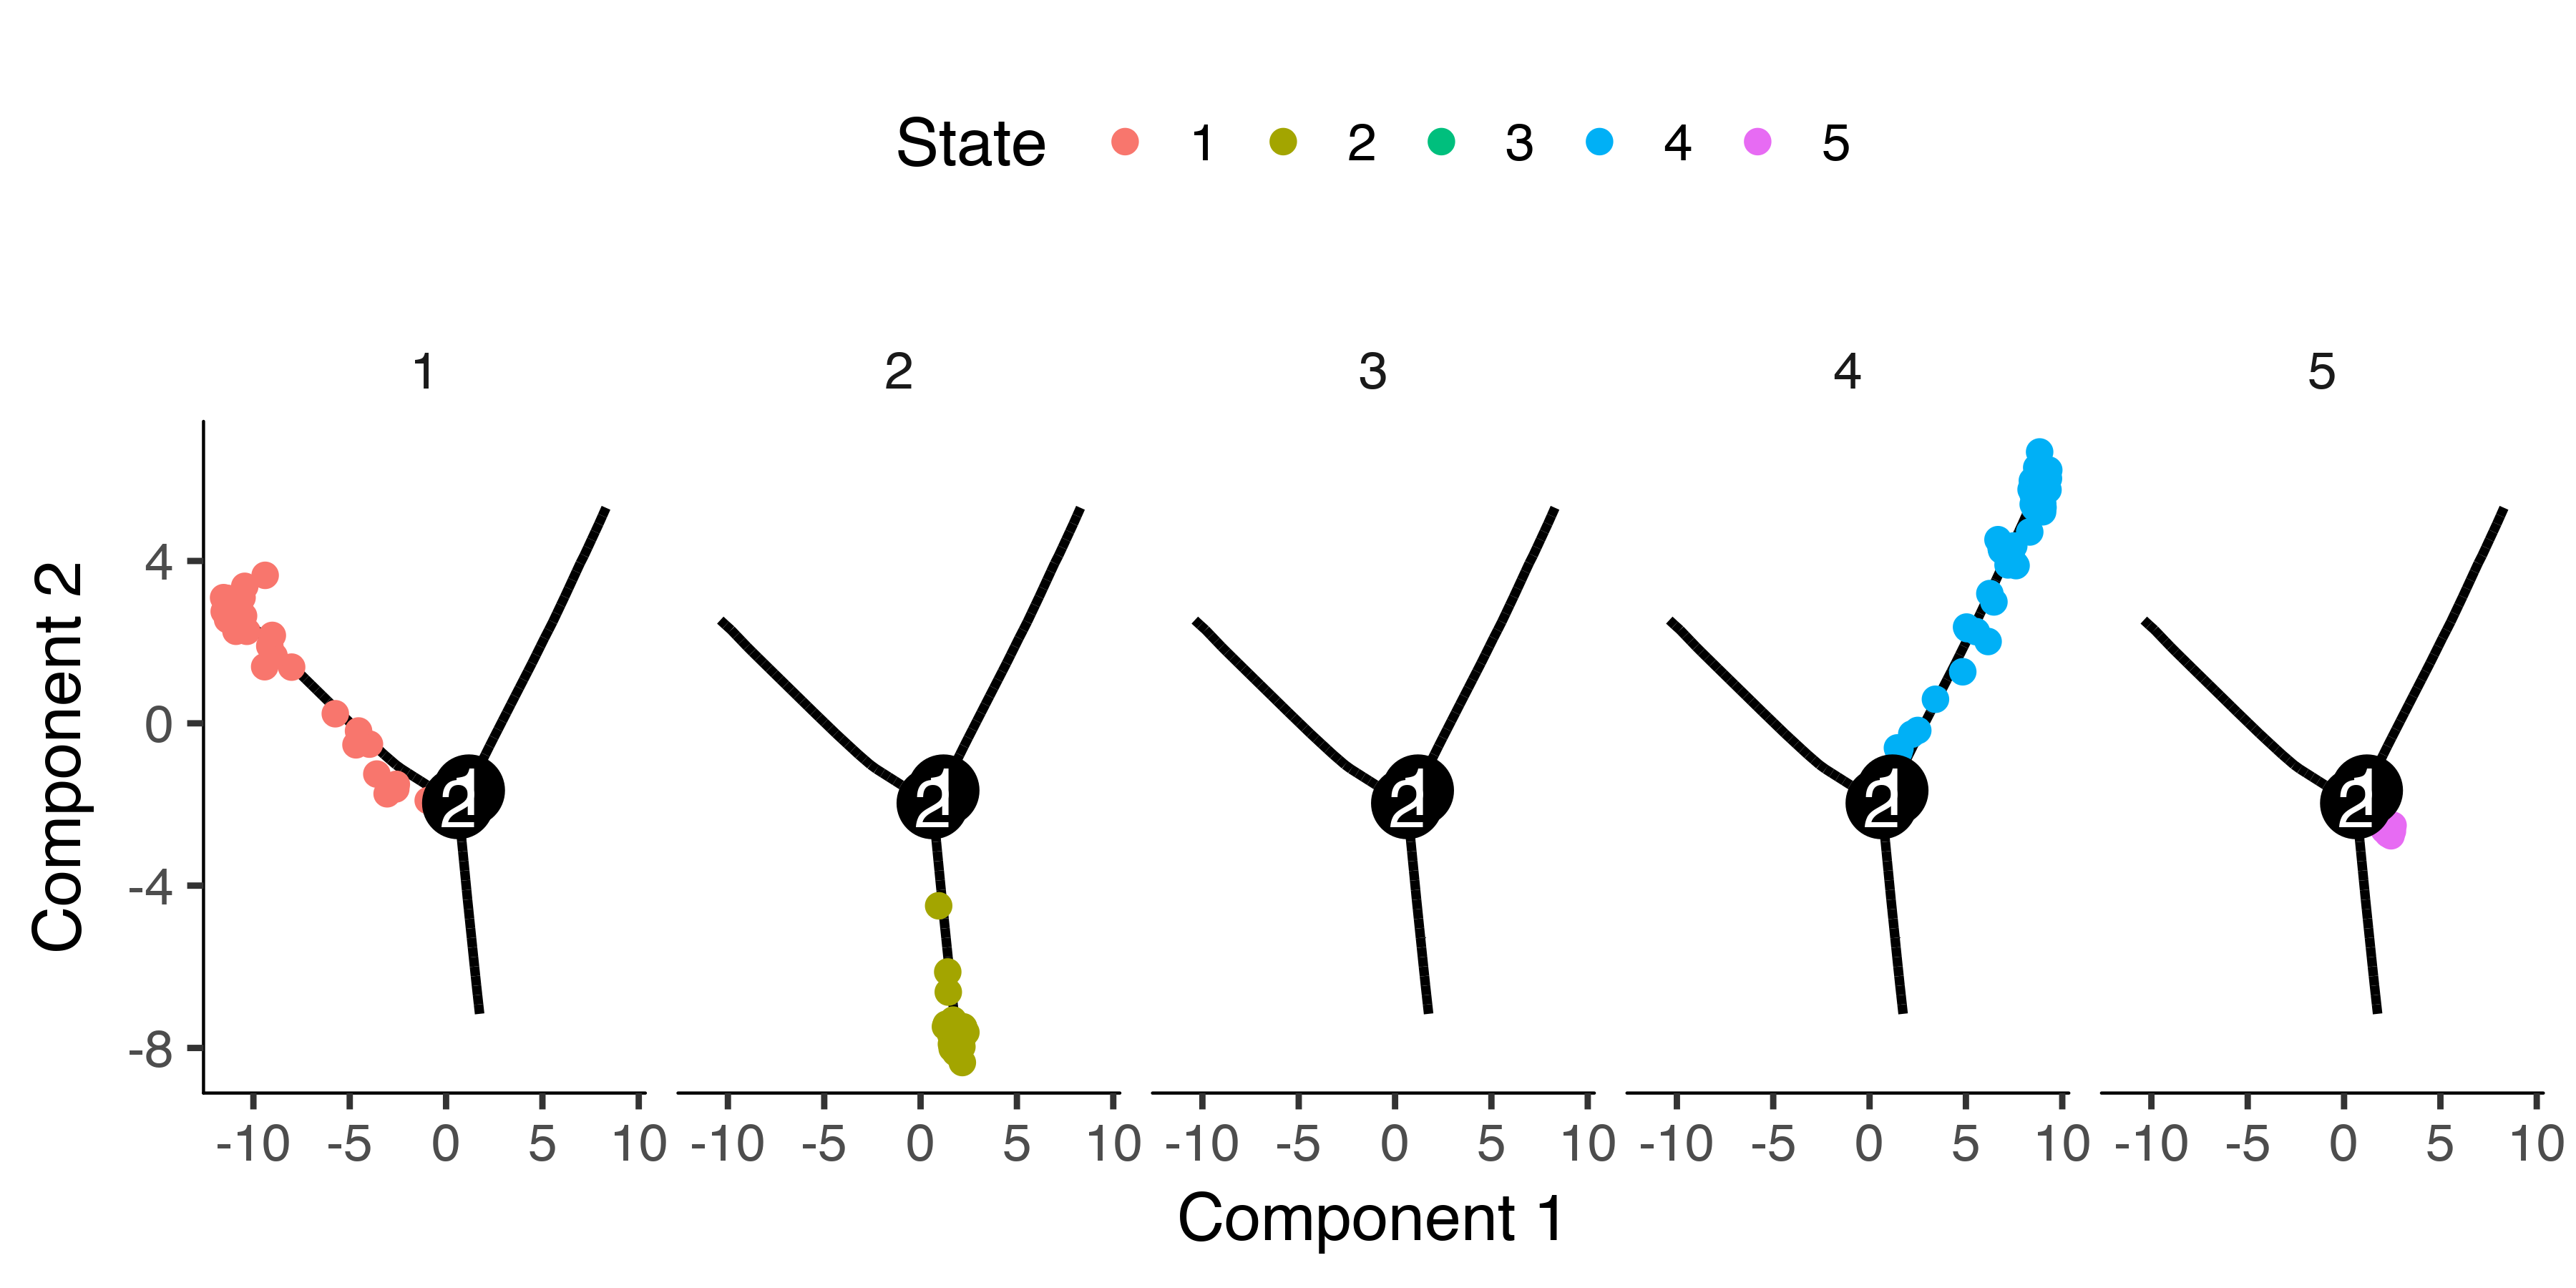
\includegraphics[width=\maxwidth]{figure/init_hsmm_facet_state-1} 

\end{knitrout}

And if you don't have a timeseries, you might need to set the root based on where certain marker genes are expressed, using your biological knowledge of the system. For example, in this experiment, a highly proliferative population of progenitor cells are generating two types of post-mitotic cells. So the root should have cells that express high levels of proliferation markers. We can use the jitter plot to pick figure out which state corresponds to rapid proliferation:

\begin{knitrout}
\definecolor{shadecolor}{rgb}{0.969, 0.969, 0.969}\color{fgcolor}\begin{kframe}
\begin{alltt}
\hlstd{blast_genes} \hlkwb{<-} \hlkwd{row.names}\hlstd{(}\hlkwd{subset}\hlstd{(}\hlkwd{fData}\hlstd{(HSMM_myo), gene_short_name} \hlopt \hlkwd{c}\hlstd{(}\hlstr{"CCNB2"}\hlstd{,} \hlstr{"MYOD1"}\hlstd{,} \hlstr{"MYOG"}\hlstd{)))}
\hlkwd{plot_genes_jitter}\hlstd{(HSMM_myo[blast_genes,],} \hlkwc{grouping}\hlstd{=}\hlstr{"State"}\hlstd{,} \hlkwc{min_expr}\hlstd{=}\hlnum{0.1}\hlstd{)}
\end{alltt}
\end{kframe}

{\centering 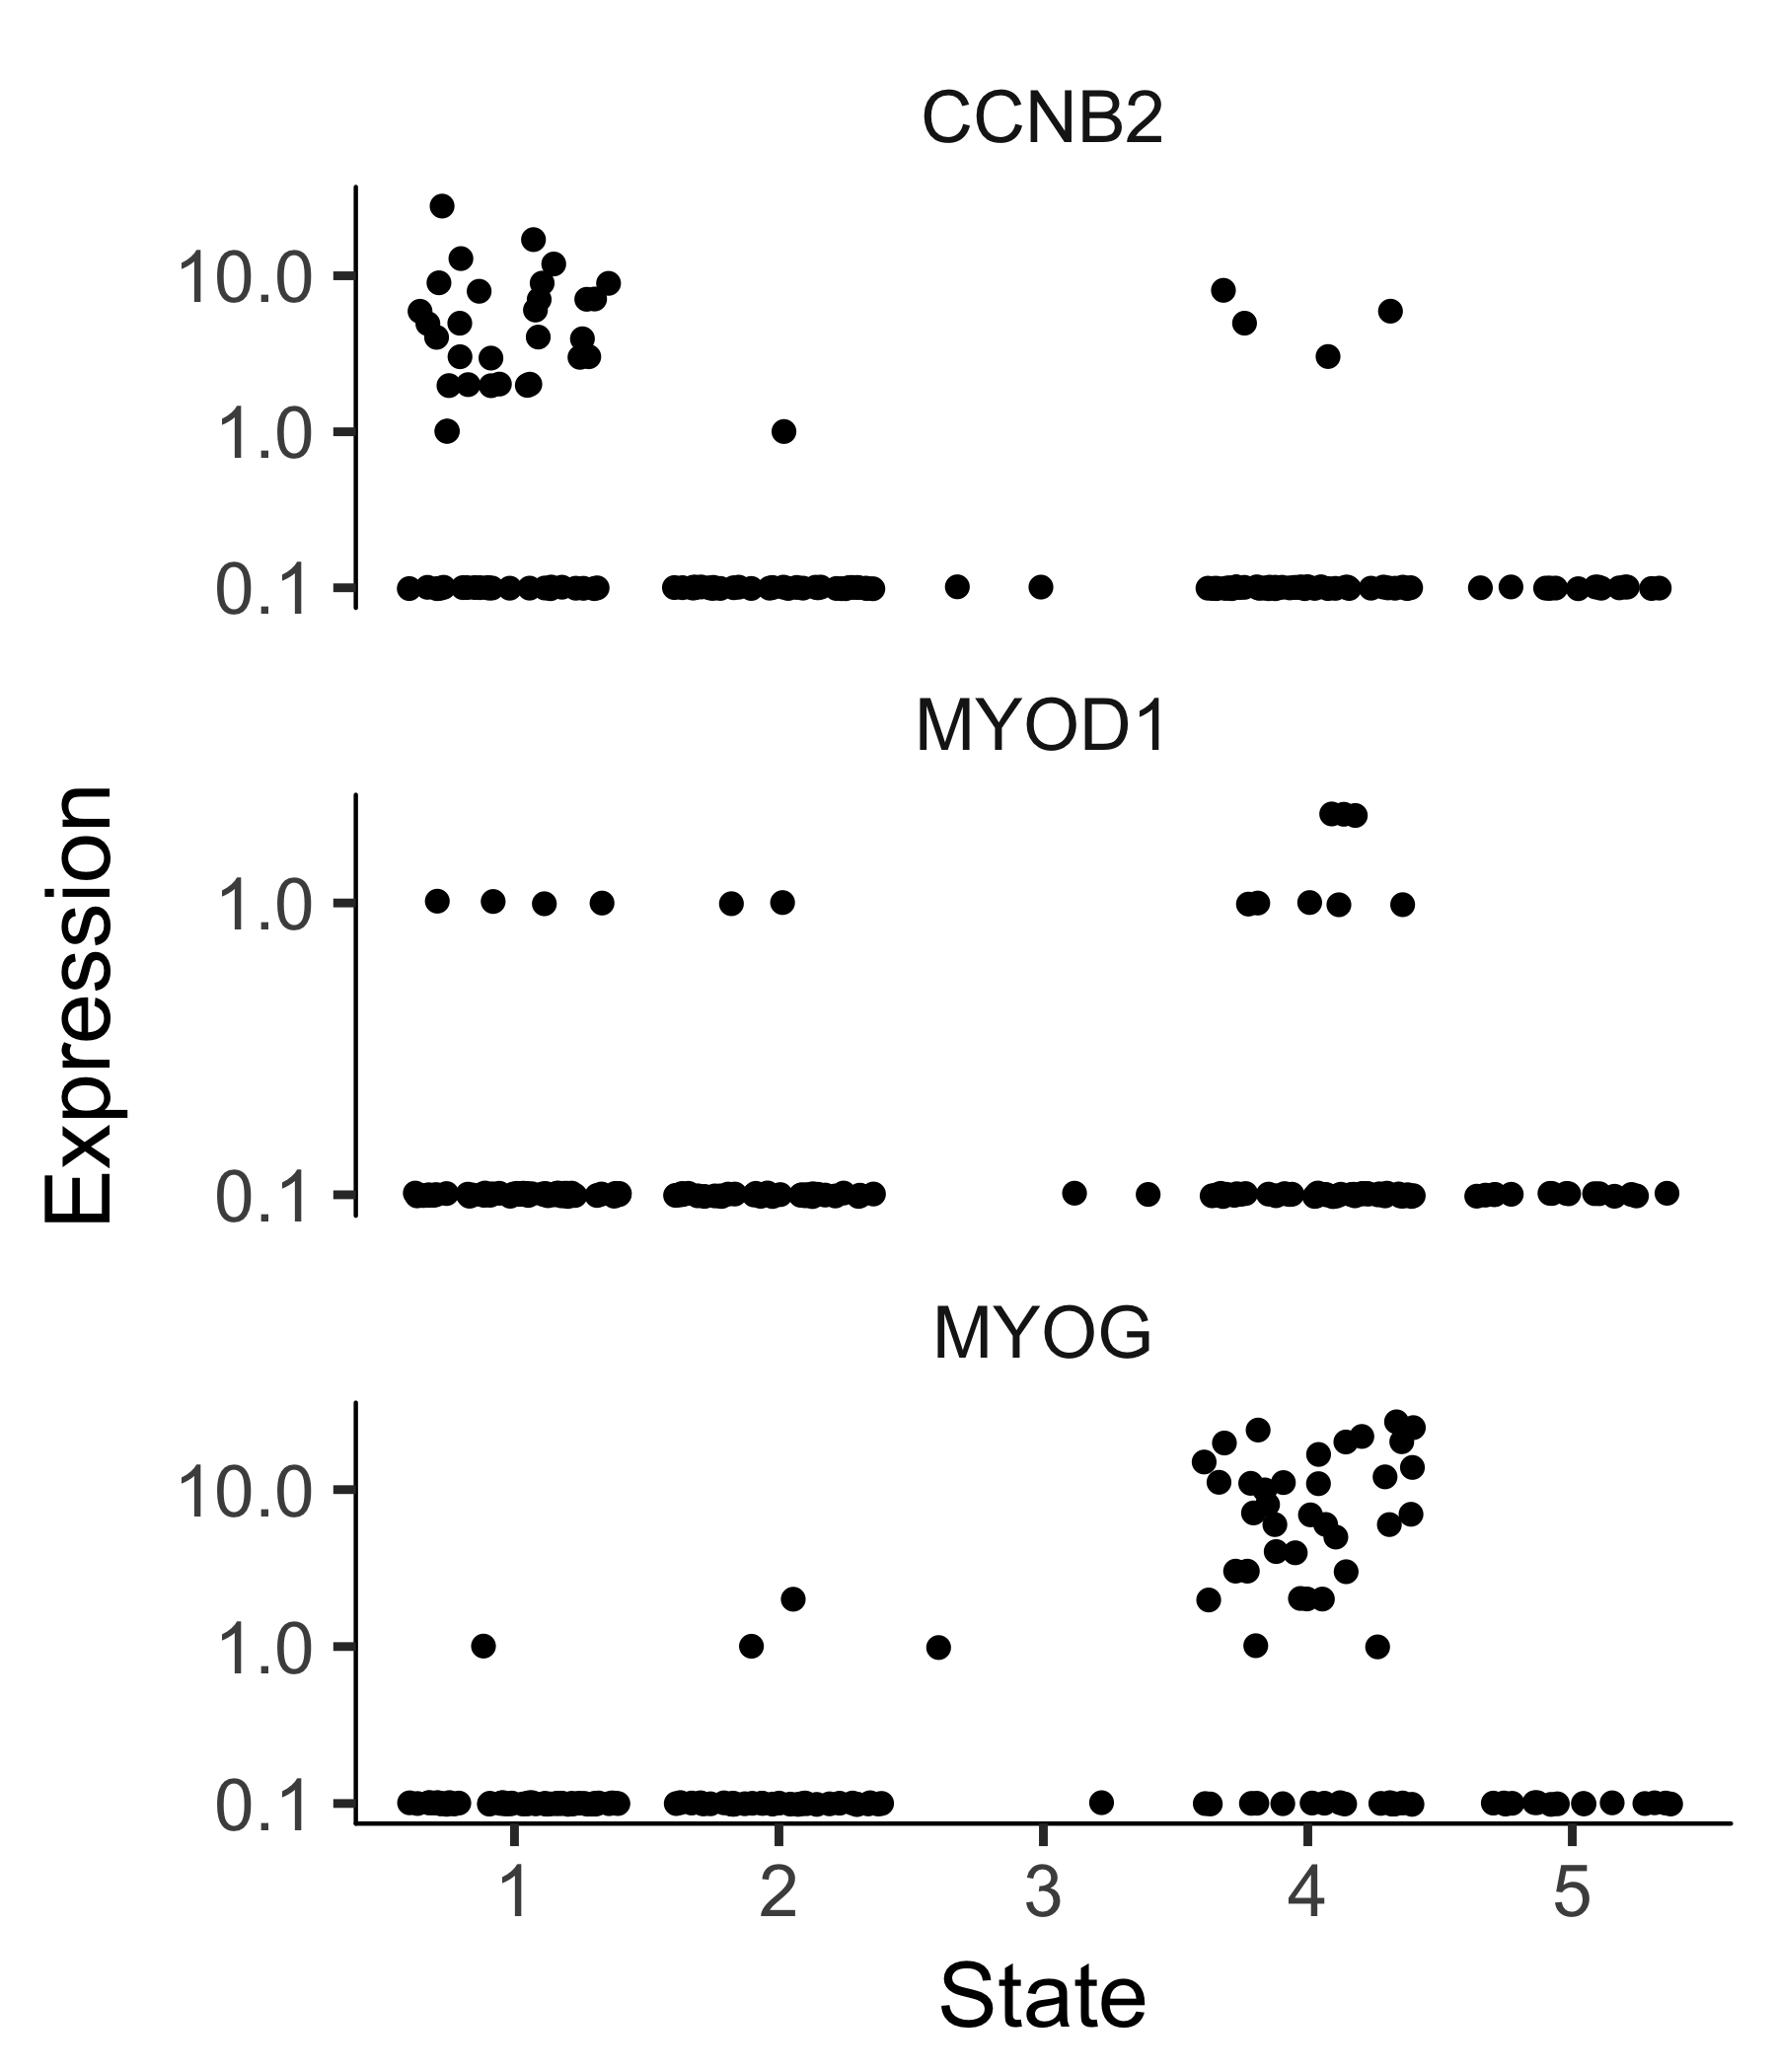
\includegraphics[width=\maxwidth]{figure/init_hsmm_jitter_state-1} 

}



\end{knitrout}


To confirm that the ordering is correct we can select a couple of markers of myogenic progress. Plotting these genes demonstrates that ordering looks good: 

\begin{knitrout}
\definecolor{shadecolor}{rgb}{0.969, 0.969, 0.969}\color{fgcolor}\begin{kframe}
\begin{alltt}
\hlstd{HSMM_expressed_genes} \hlkwb{<-}  \hlkwd{row.names}\hlstd{(}\hlkwd{subset}\hlstd{(}\hlkwd{fData}\hlstd{(HSMM_myo), num_cells_expressed} \hlopt{>=} \hlnum{10}\hlstd{))}
\hlstd{HSMM_filtered} \hlkwb{<-} \hlstd{HSMM_myo[HSMM_expressed_genes,]}

\hlstd{my_genes} \hlkwb{<-} \hlkwd{row.names}\hlstd{(}\hlkwd{subset}\hlstd{(}\hlkwd{fData}\hlstd{(HSMM_filtered),}
                              \hlstd{gene_short_name} \hlopt \hlkwd{c}\hlstd{(}\hlstr{"CDK1"}\hlstd{,} \hlstr{"MEF2C"}\hlstd{,} \hlstr{"MYH3"}\hlstd{)))}

\hlstd{cds_subset} \hlkwb{<-} \hlstd{HSMM_filtered[my_genes,]}
\hlkwd{plot_genes_in_pseudotime}\hlstd{(cds_subset,} \hlkwc{color_by}\hlstd{=}\hlstr{"Hours"}\hlstd{)}
\end{alltt}
\end{kframe}

{\centering 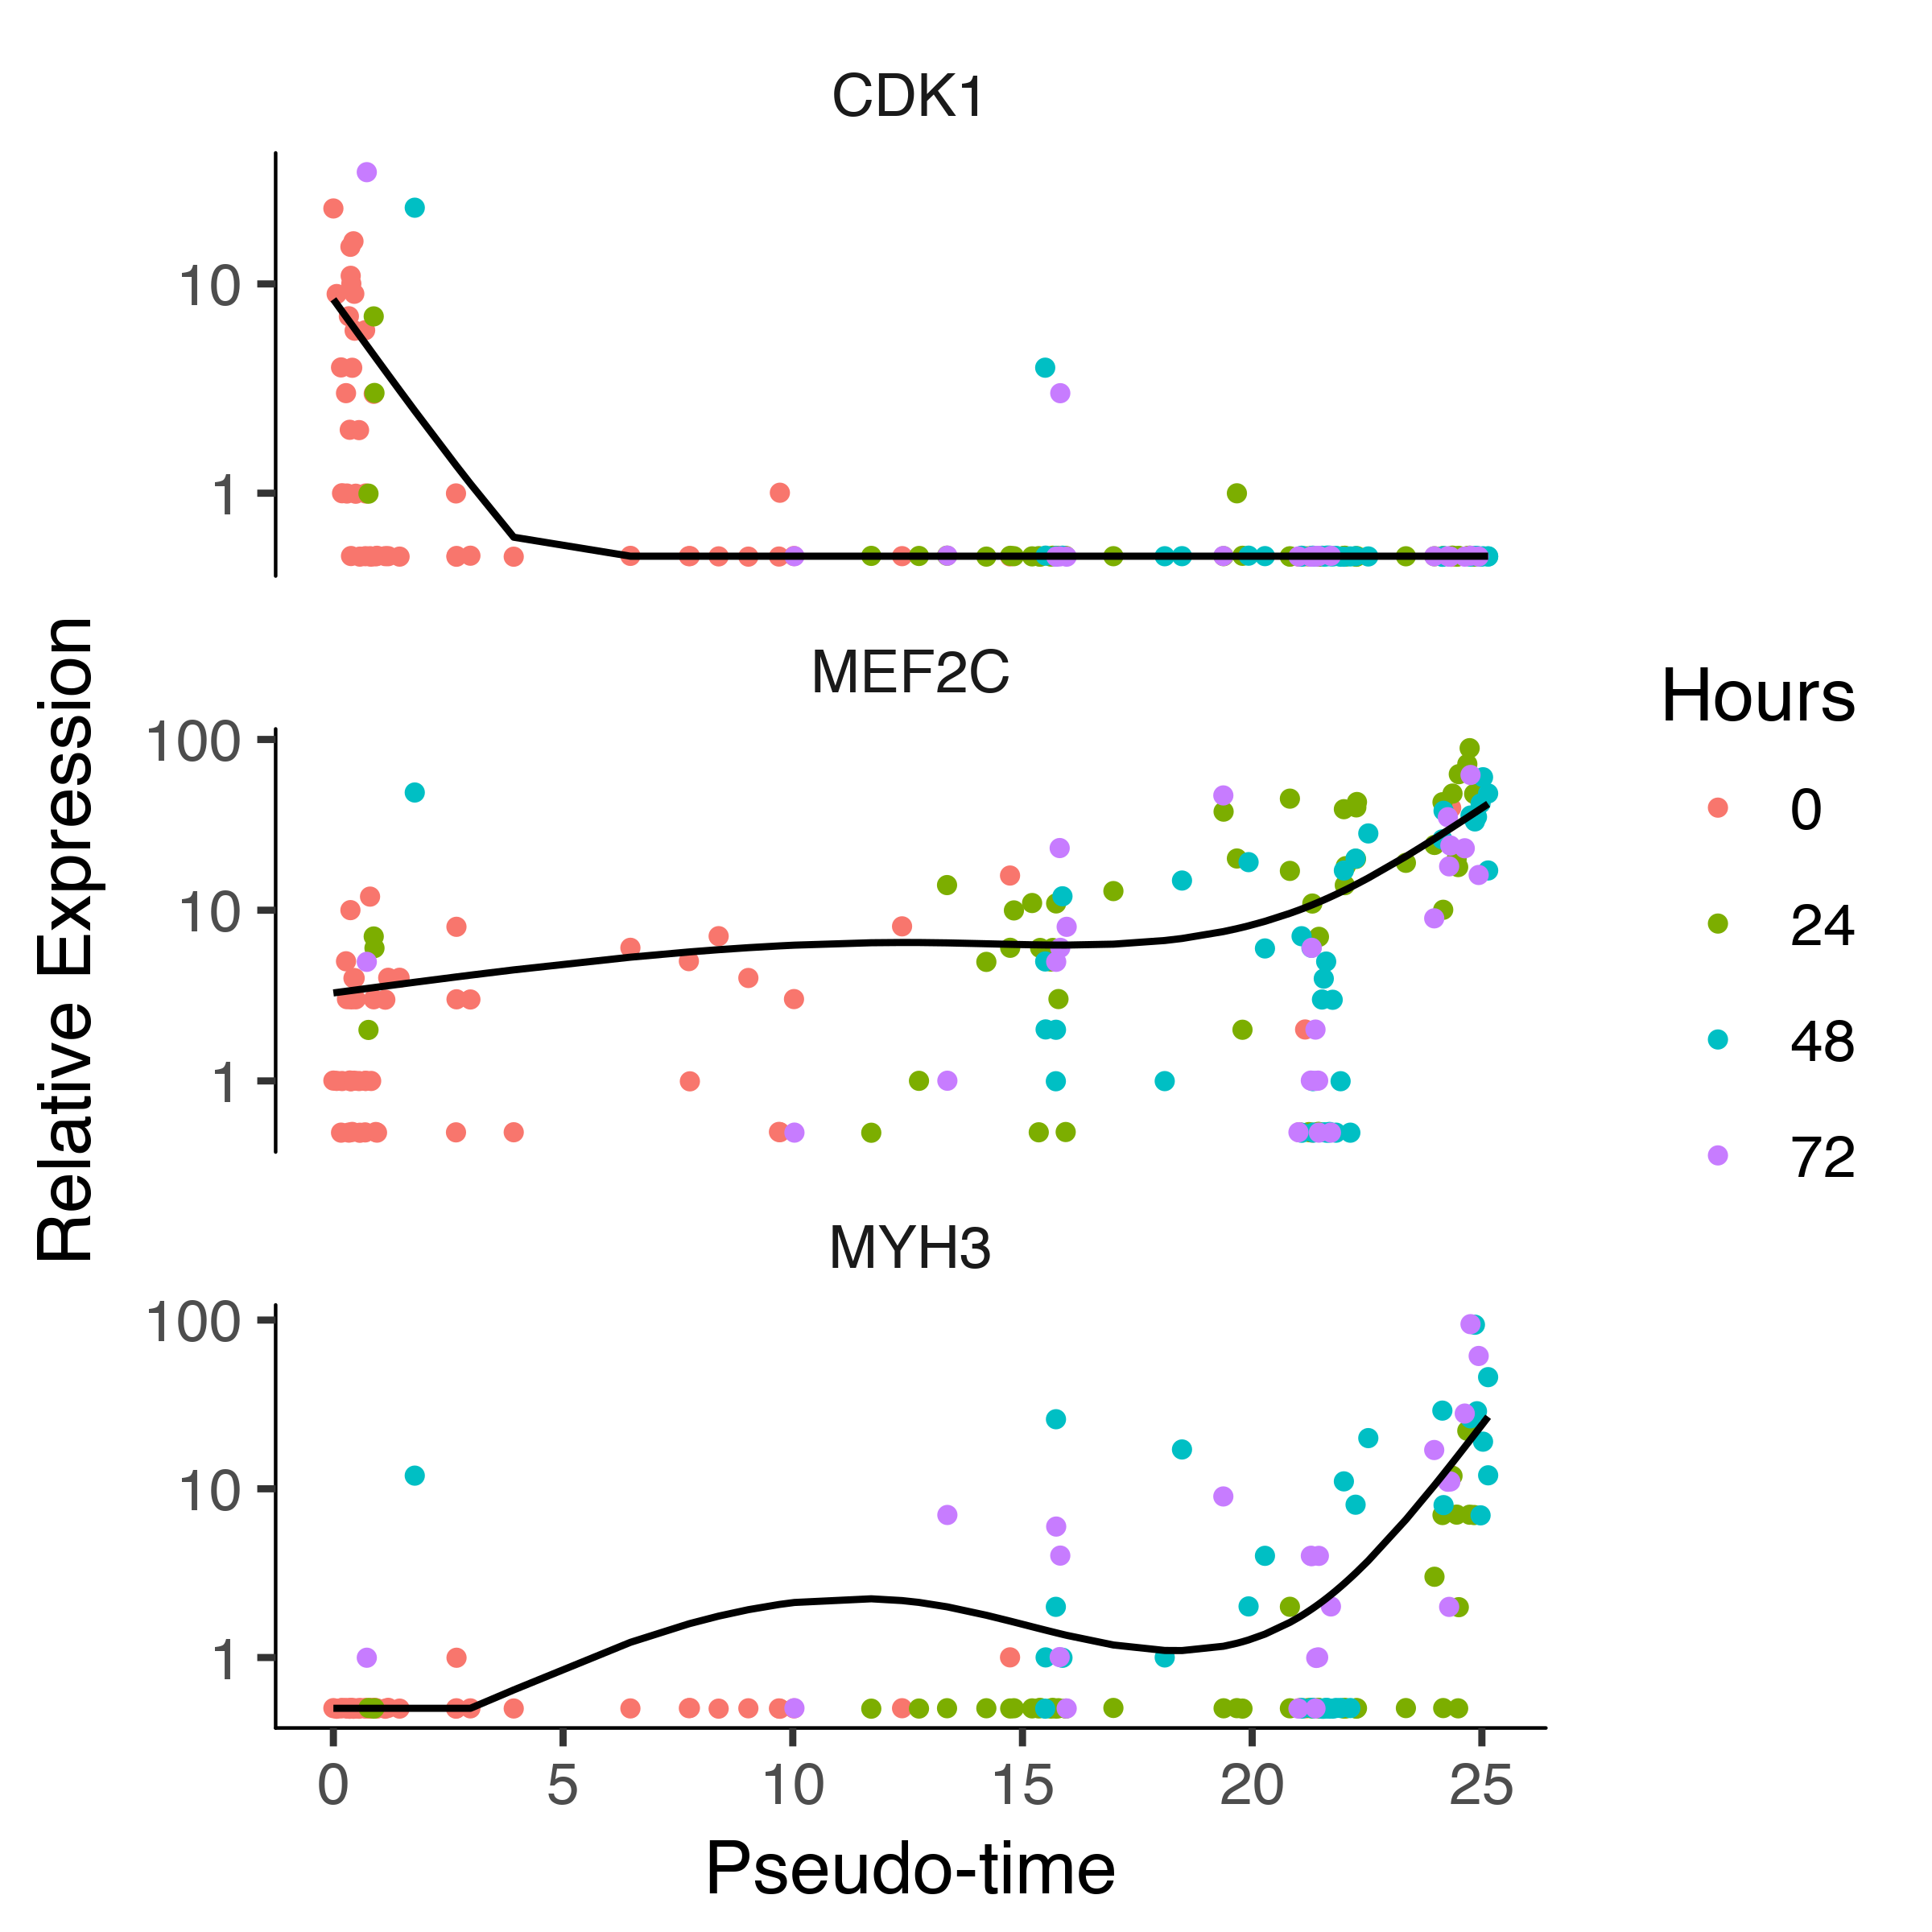
\includegraphics[width=\maxwidth]{figure/plot_markers_linear-1} 

}



\end{knitrout}

\textbf{Note:} in the event that Monocle produces a linear trajectory, there will only
be one state. In this case, you can tell it which end is the beginning of the 
trajectory by passing \Rfunction{orderCells} an optional argument argument: the 
\Robject{reverse} flag. The \Robject{reverse} flag tells Monocle to reverse the 
orientation of the entire process as it's being discovered from the data, 
so that the cells that would have been assigned to the end are instead assigned 
to the beginning, and so on.  

\subsubsection{Selecting genes based on PCA loading}

A number of single-cell clustering studies have found that principal component
analysis (PCA) is an effective way of finding genes that vary widely across cells. You 
can use PCA to pick out a good set of ordering genes in a completely unsupervised
manner. The procedure below first normalizes the expression data by adding a 
pseudocount, log-transforming it, and then standardizing it so that all genes
have roughly the same dynamic range.  Then, it uses the \Rpackage{irlba} package
to perform the PCA. The code below is a little more complicated than just calling
\Rfunction{prcomp()}, but it has the advantage of performing the entire computation
with sparse matrix operations. This is important for large, sparse CellDataSet 
objects like the ones common in droplet-based single-cell RNA-Seq.

\begin{knitrout}
\definecolor{shadecolor}{rgb}{0.969, 0.969, 0.969}\color{fgcolor}\begin{kframe}
\begin{alltt}
\hlstd{HSMM_myo} \hlkwb{<-} \hlstd{HSMM_myo[HSMM_expressed_genes,]}
\hlstd{exprs_filtered} \hlkwb{<-} \hlkwd{t}\hlstd{(}\hlkwd{t}\hlstd{(}\hlkwd{exprs}\hlstd{(HSMM_myo)}\hlopt{/}\hlkwd{pData}\hlstd{(HSMM_myo)}\hlopt{$}\hlstd{Size_Factor))}
\hlcom{#nz_genes <- which(exprs_filtered != 0, arr.ind = T)}
\hlstd{exprs_filtered}\hlopt{@}\hlkwc{x} \hlkwb{<-} \hlkwd{log}\hlstd{(exprs_filtered}\hlopt{@}\hlkwc{x} \hlopt{+} \hlnum{1}\hlstd{)}

\hlcom{# Calculate the variance across genes without converting to a dense}
\hlcom{# matrix:}
\hlstd{expression_means} \hlkwb{<-} \hlstd{Matrix}\hlopt{::}\hlkwd{rowMeans}\hlstd{(exprs_filtered)}
\hlstd{expression_vars} \hlkwb{<-} \hlstd{Matrix}\hlopt{::}\hlkwd{rowMeans}\hlstd{((exprs_filtered} \hlopt{-} \hlstd{expression_means)}\hlopt{^}\hlnum{2}\hlstd{)}

\hlcom{# Filter out genes that are constant across all cells:}
\hlstd{genes_to_keep} \hlkwb{<-} \hlstd{expression_vars} \hlopt{>} \hlnum{0}
\hlstd{exprs_filtered} \hlkwb{<-} \hlstd{exprs_filtered[genes_to_keep,]}
\hlstd{expression_means} \hlkwb{<-} \hlstd{expression_means[genes_to_keep]}
\hlstd{expression_vars} \hlkwb{<-} \hlstd{expression_vars[genes_to_keep]}

\hlcom{# Here's how to take the top PCA loading genes, but using}
\hlcom{# sparseMatrix operations the whole time, using irlba. Note}
\hlcom{# that the v matrix from irlba is the loading matrix}
\hlkwd{set.seed}\hlstd{(}\hlnum{0}\hlstd{)}
\hlstd{irlba_pca_res} \hlkwb{<-} \hlkwd{irlba}\hlstd{(}\hlkwd{t}\hlstd{(exprs_filtered),}
                      \hlkwc{nu}\hlstd{=}\hlnum{0}\hlstd{,}
                      \hlkwc{center}\hlstd{=expression_means,}
                      \hlkwc{scale}\hlstd{=}\hlkwd{sqrt}\hlstd{(expression_vars),}
                      \hlkwc{right_only}\hlstd{=}\hlnum{TRUE}\hlstd{)}\hlopt{$}\hlstd{v}

\hlkwd{row.names}\hlstd{(irlba_pca_res)} \hlkwb{<-} \hlkwd{row.names}\hlstd{(exprs_filtered)}

\hlcom{# Here, we will just}
\hlcom{# take the top 200 genes from components 2 and 3. }
\hlcom{# Component 1 usually is driven by technical noise.}
\hlcom{# We could also use a more principled approach, }
\hlcom{# similar to what dpFeature does below}
\hlstd{PC2_genes} \hlkwb{<-} \hlkwd{names}\hlstd{(}\hlkwd{sort}\hlstd{(}\hlkwd{abs}\hlstd{(irlba_pca_res[,} \hlnum{2}\hlstd{]),} \hlkwc{decreasing} \hlstd{= T))[}\hlnum{1}\hlopt{:}\hlnum{200}\hlstd{]}
\hlstd{PC3_genes} \hlkwb{<-} \hlkwd{names}\hlstd{(}\hlkwd{sort}\hlstd{(}\hlkwd{abs}\hlstd{(irlba_pca_res[,} \hlnum{3}\hlstd{]),} \hlkwc{decreasing} \hlstd{= T))[}\hlnum{1}\hlopt{:}\hlnum{200}\hlstd{]}

\hlstd{ordering_genes} \hlkwb{<-} \hlkwd{union}\hlstd{(PC2_genes, PC3_genes)}
\end{alltt}
\end{kframe}
\end{knitrout}

Using these to order the cells as above yields the following trajectory:
\begin{knitrout}
\definecolor{shadecolor}{rgb}{0.969, 0.969, 0.969}\color{fgcolor}\begin{kframe}
\begin{alltt}
\hlstd{HSMM_myo} \hlkwb{<-} \hlkwd{setOrderingFilter}\hlstd{(HSMM_myo, ordering_genes)}
\hlstd{HSMM_myo} \hlkwb{<-} \hlkwd{reduceDimension}\hlstd{(HSMM_myo,} \hlkwc{max_components}\hlstd{=}\hlnum{2}\hlstd{,} \hlkwc{method} \hlstd{=} \hlstr{'DDRTree'}\hlstd{)}
\hlstd{HSMM_myo} \hlkwb{<-} \hlkwd{orderCells}\hlstd{(HSMM_myo)}
\hlstd{HSMM_myo} \hlkwb{<-} \hlkwd{orderCells}\hlstd{(HSMM_myo,} \hlkwc{root_state}\hlstd{=}\hlkwd{GM_state}\hlstd{(HSMM_myo))}
\hlkwd{plot_cell_trajectory}\hlstd{(HSMM_myo,} \hlkwc{color_by}\hlstd{=}\hlstr{"Hours"}\hlstd{)}
\end{alltt}
\end{kframe}

{\centering 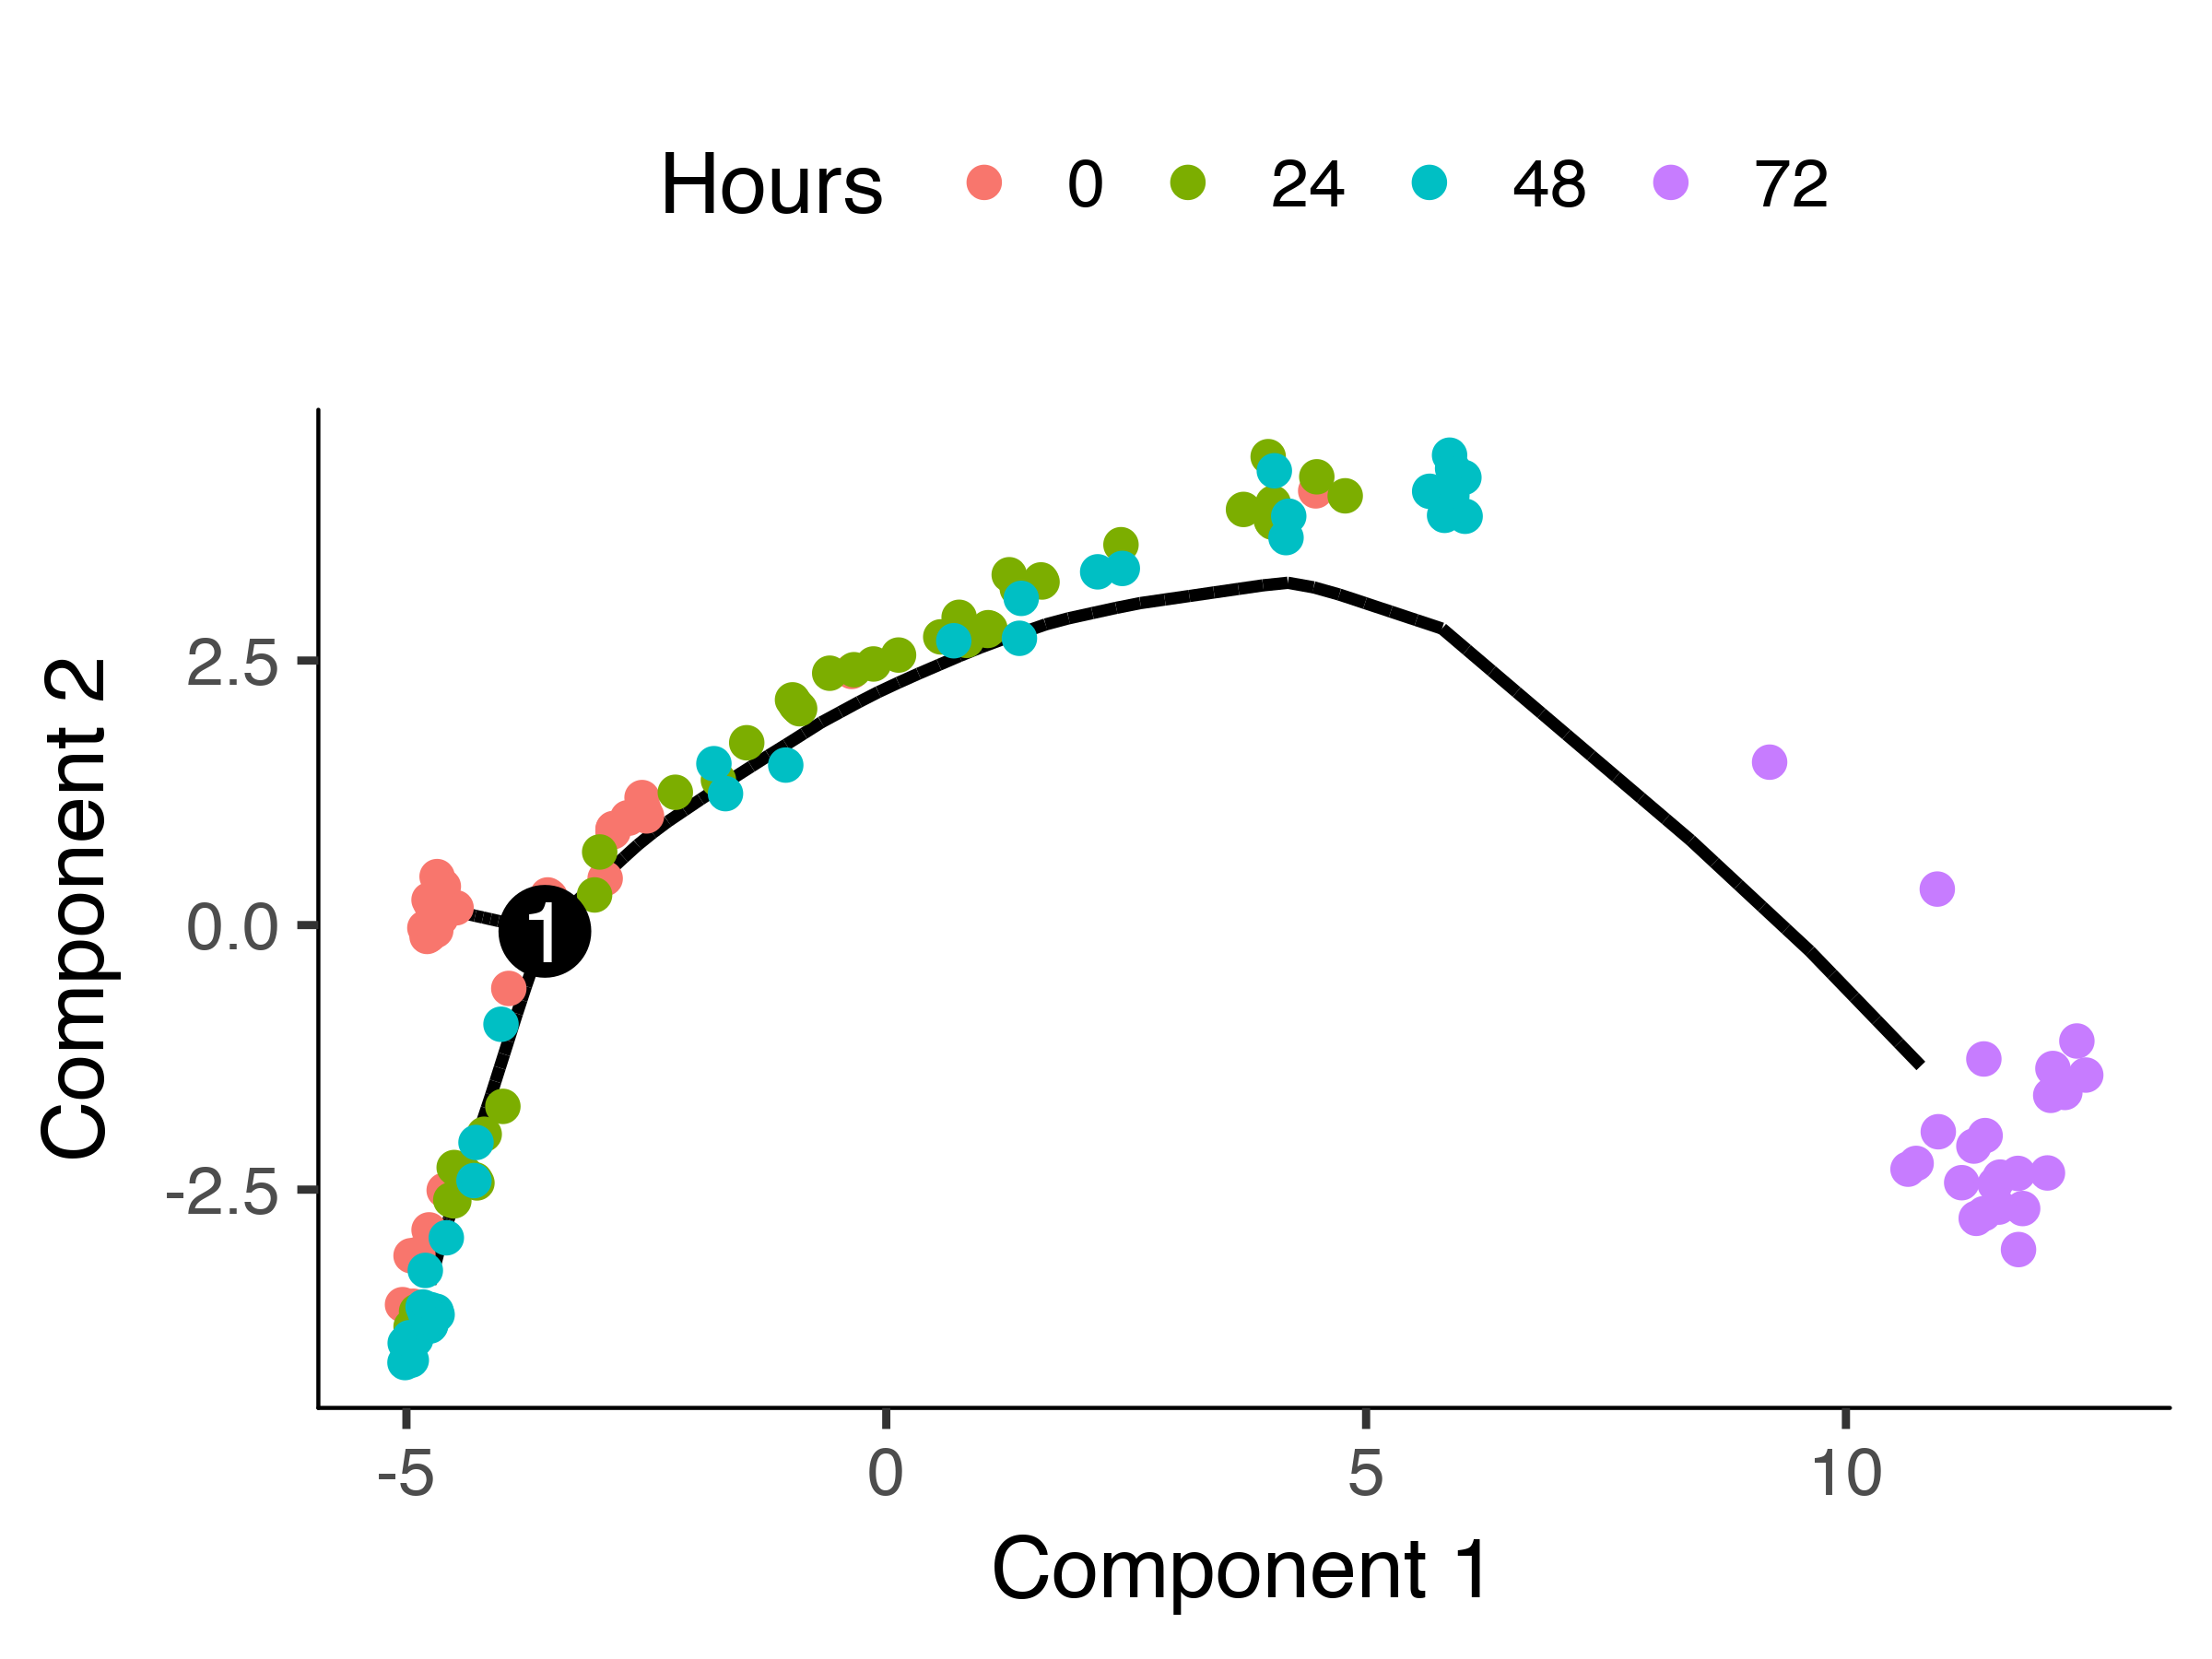
\includegraphics[width=\maxwidth]{figure/order_cells_pca_unsup-1} 

}



\end{knitrout}

\subsection{Unsupervised feature selection based on density peak clustering}
Selecting genes for ordering cells using the techniques discussed above often 
works well in simple settings, but for more complex processes, we recommend a 
new procedure called ``dpFeature''. This procedure works by first projecting 
cells into two dimensions using t-SNE and then detecting clusters using the 
``densityPeak'' algorithm of Rodriguez and Laio \cite{RodriguezLaio}. The 
resulting clusters of cells are compared using Monocle's differential expression
analysis functions to find genes that distinguish them. The top of these are 
then used to order cells.

To use dpFeature, we first select superset of feature genes as genes expressed 
in at least $5\%$ of all the cells. 
\begin{knitrout}
\definecolor{shadecolor}{rgb}{0.969, 0.969, 0.969}\color{fgcolor}\begin{kframe}
\begin{alltt}
\hlstd{HSMM_myo} \hlkwb{<-} \hlkwd{detectGenes}\hlstd{(HSMM_myo,} \hlkwc{min_expr}\hlstd{=}\hlnum{0.1}\hlstd{)}
\hlkwd{fData}\hlstd{(HSMM_myo)}\hlopt{$}\hlstd{use_for_ordering} \hlkwb{<-} \hlkwd{fData}\hlstd{(HSMM_myo)}\hlopt{$}\hlstd{num_cells_expressed} \hlopt{>} \hlnum{0.05} \hlopt{*} \hlkwd{ncol}\hlstd{(HSMM_myo)}
\end{alltt}
\end{kframe}
\end{knitrout}

Then we will perform a PCA analysis to identify the variance explained by each PC (principal component). 
We can look at a scree plot and determine how many pca dimensions are wanted based on whether or not there is a 
significant gap between that component and the component after it. By selecting only the high loading PCs, 
we effectively only focus on the more interesting biological variations.  
\begin{knitrout}
\definecolor{shadecolor}{rgb}{0.969, 0.969, 0.969}\color{fgcolor}\begin{kframe}
\begin{alltt}
\hlkwd{plot_pc_variance_explained}\hlstd{(HSMM_myo,} \hlkwc{return_all} \hlstd{= F)} \hlcom{#look at the plot and decide how many dimensions you need. It is determined by a huge drop of variance at that dimension. pass that number to num_dim in the next function.}
\end{alltt}
\end{kframe}

{\centering 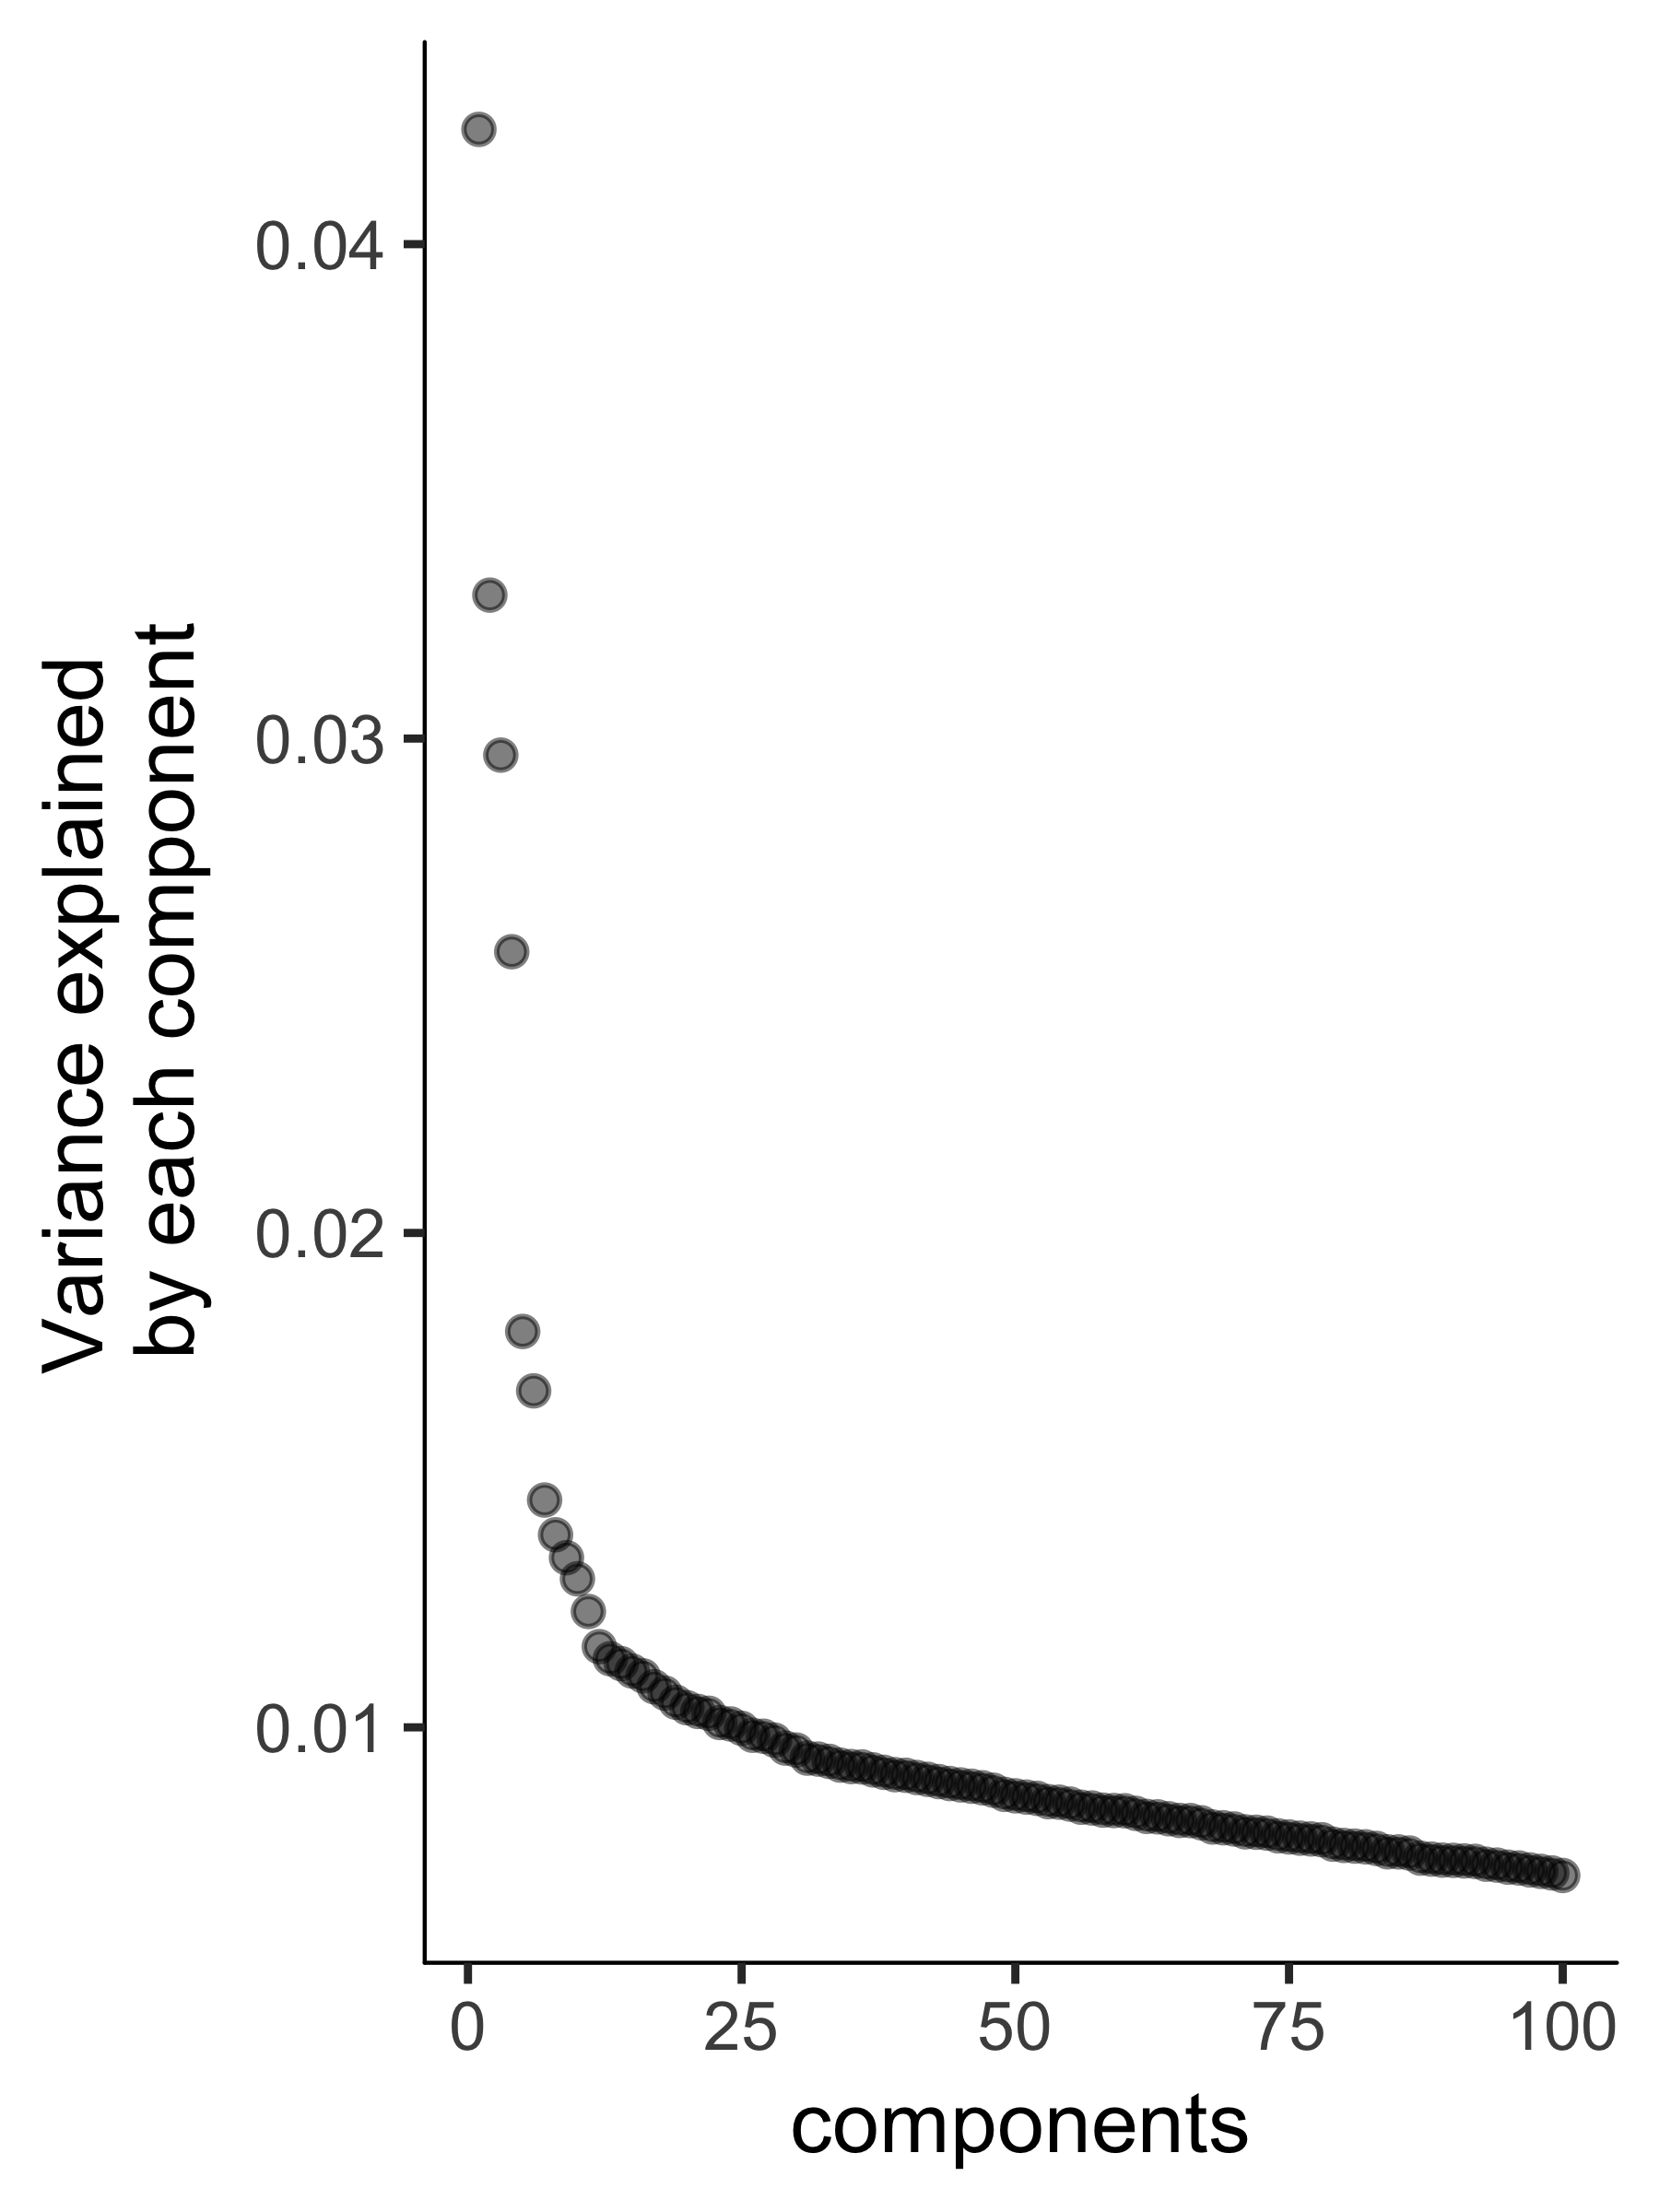
\includegraphics[width=\maxwidth]{figure/plot_pc_variance-1} 

}



\end{knitrout}

We will then run reduceDimension with t-SNE as the reduction method on those top PCs and project them further down to two dimensions.  
\begin{knitrout}
\definecolor{shadecolor}{rgb}{0.969, 0.969, 0.969}\color{fgcolor}\begin{kframe}
\begin{alltt}
  \hlstd{HSMM_myo} \hlkwb{<-} \hlkwd{reduceDimension}\hlstd{(HSMM_myo,} \hlkwc{max_components}\hlstd{=}\hlnum{2}\hlstd{,} \hlkwc{norm_method} \hlstd{=} \hlstr{'log'}\hlstd{,} \hlkwc{num_dim} \hlstd{=} \hlnum{3}\hlstd{,}
                              \hlkwc{reduction_method} \hlstd{=} \hlstr{'tSNE'}\hlstd{,} \hlkwc{verbose} \hlstd{= T)}
\end{alltt}


{\ttfamily\noindent\itshape\color{messagecolor}{\#\# Remove noise by PCA ...}}

{\ttfamily\noindent\itshape\color{messagecolor}{\#\# Reduce dimension by tSNE ...}}\end{kframe}
\end{knitrout}

Then we can run density peak clustering to identify the clusters on the 2-D t-SNE space. Density peak algorithm clusters cells based on each 
cell's local density ($\rho$) and the nearest distance $\delta$ of a cell to another cell with higher distance. We can set a threshold for 
the $\rho, \delta$ and define any cell with a higher local density and distance than the thresholds as the density peaks. Those peaks are then 
used to define the clusters for all cells. By default, \Rfunction{clusterCells} choose $95\%$ of $\rho$ and $\delta$ to define 
the thresholds. We can also set a number of clusters ($n$) we want to cluster. In this setting, we will find the top $n$ cells with high 
$\delta$ with $\rho$ among the top $50\%$ range. The default setting often gives good clustering. 

\begin{knitrout}
\definecolor{shadecolor}{rgb}{0.969, 0.969, 0.969}\color{fgcolor}\begin{kframe}
\begin{alltt}
\hlstd{HSMM_myo} \hlkwb{<-} \hlkwd{clusterCells}\hlstd{(HSMM_myo,} \hlkwc{verbose} \hlstd{= F)}
\end{alltt}
\begin{verbatim}
## Distance cutoff calculated to 0.681014
\end{verbatim}


{\ttfamily\noindent\itshape\color{messagecolor}{\#\# the length of the distance: 11935}}\end{kframe}
\end{knitrout}

After the clustering, we can check the clustering results. 
\begin{knitrout}
\definecolor{shadecolor}{rgb}{0.969, 0.969, 0.969}\color{fgcolor}\begin{kframe}
\begin{alltt}
\hlkwd{plot_cell_clusters}\hlstd{(HSMM_myo,} \hlkwc{color_by} \hlstd{=} \hlstr{'as.factor(Cluster)'}\hlstd{)}
\hlkwd{plot_cell_clusters}\hlstd{(HSMM_myo,} \hlkwc{color_by} \hlstd{=} \hlstr{'as.factor(Hours)'}\hlstd{)}
\end{alltt}
\end{kframe}
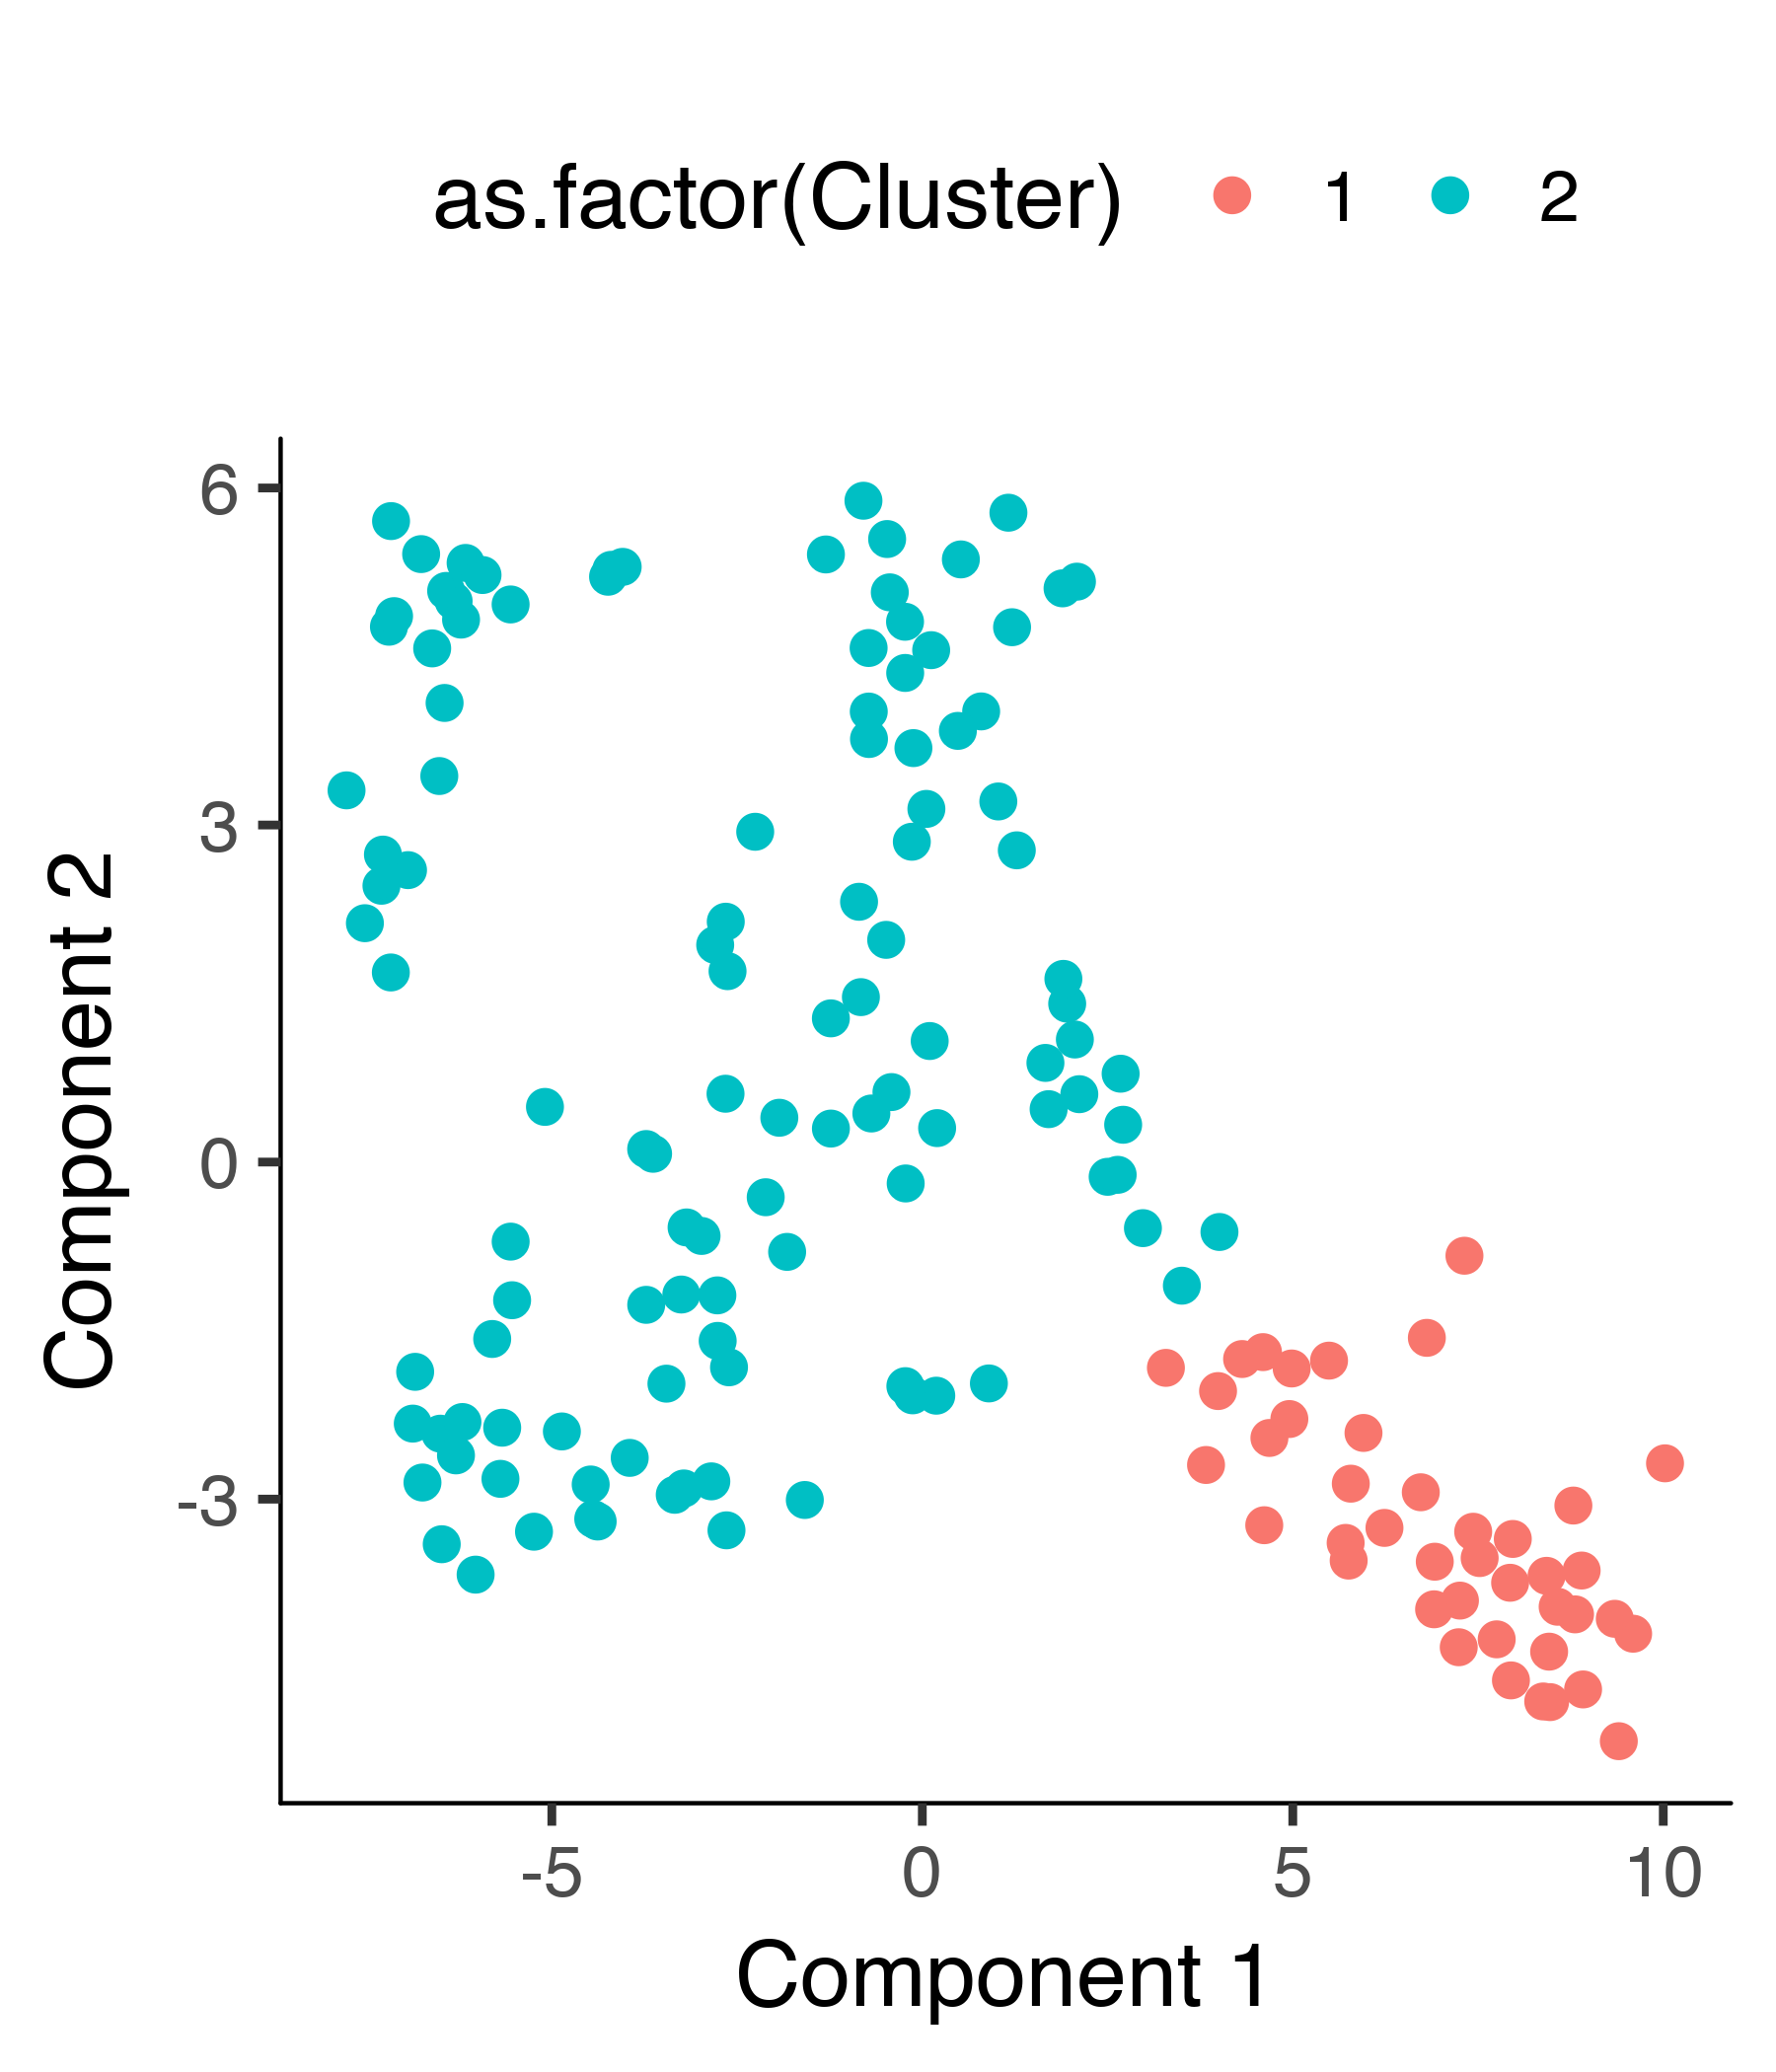
\includegraphics[width=\maxwidth]{figure/check_the_clustering_results-1} 
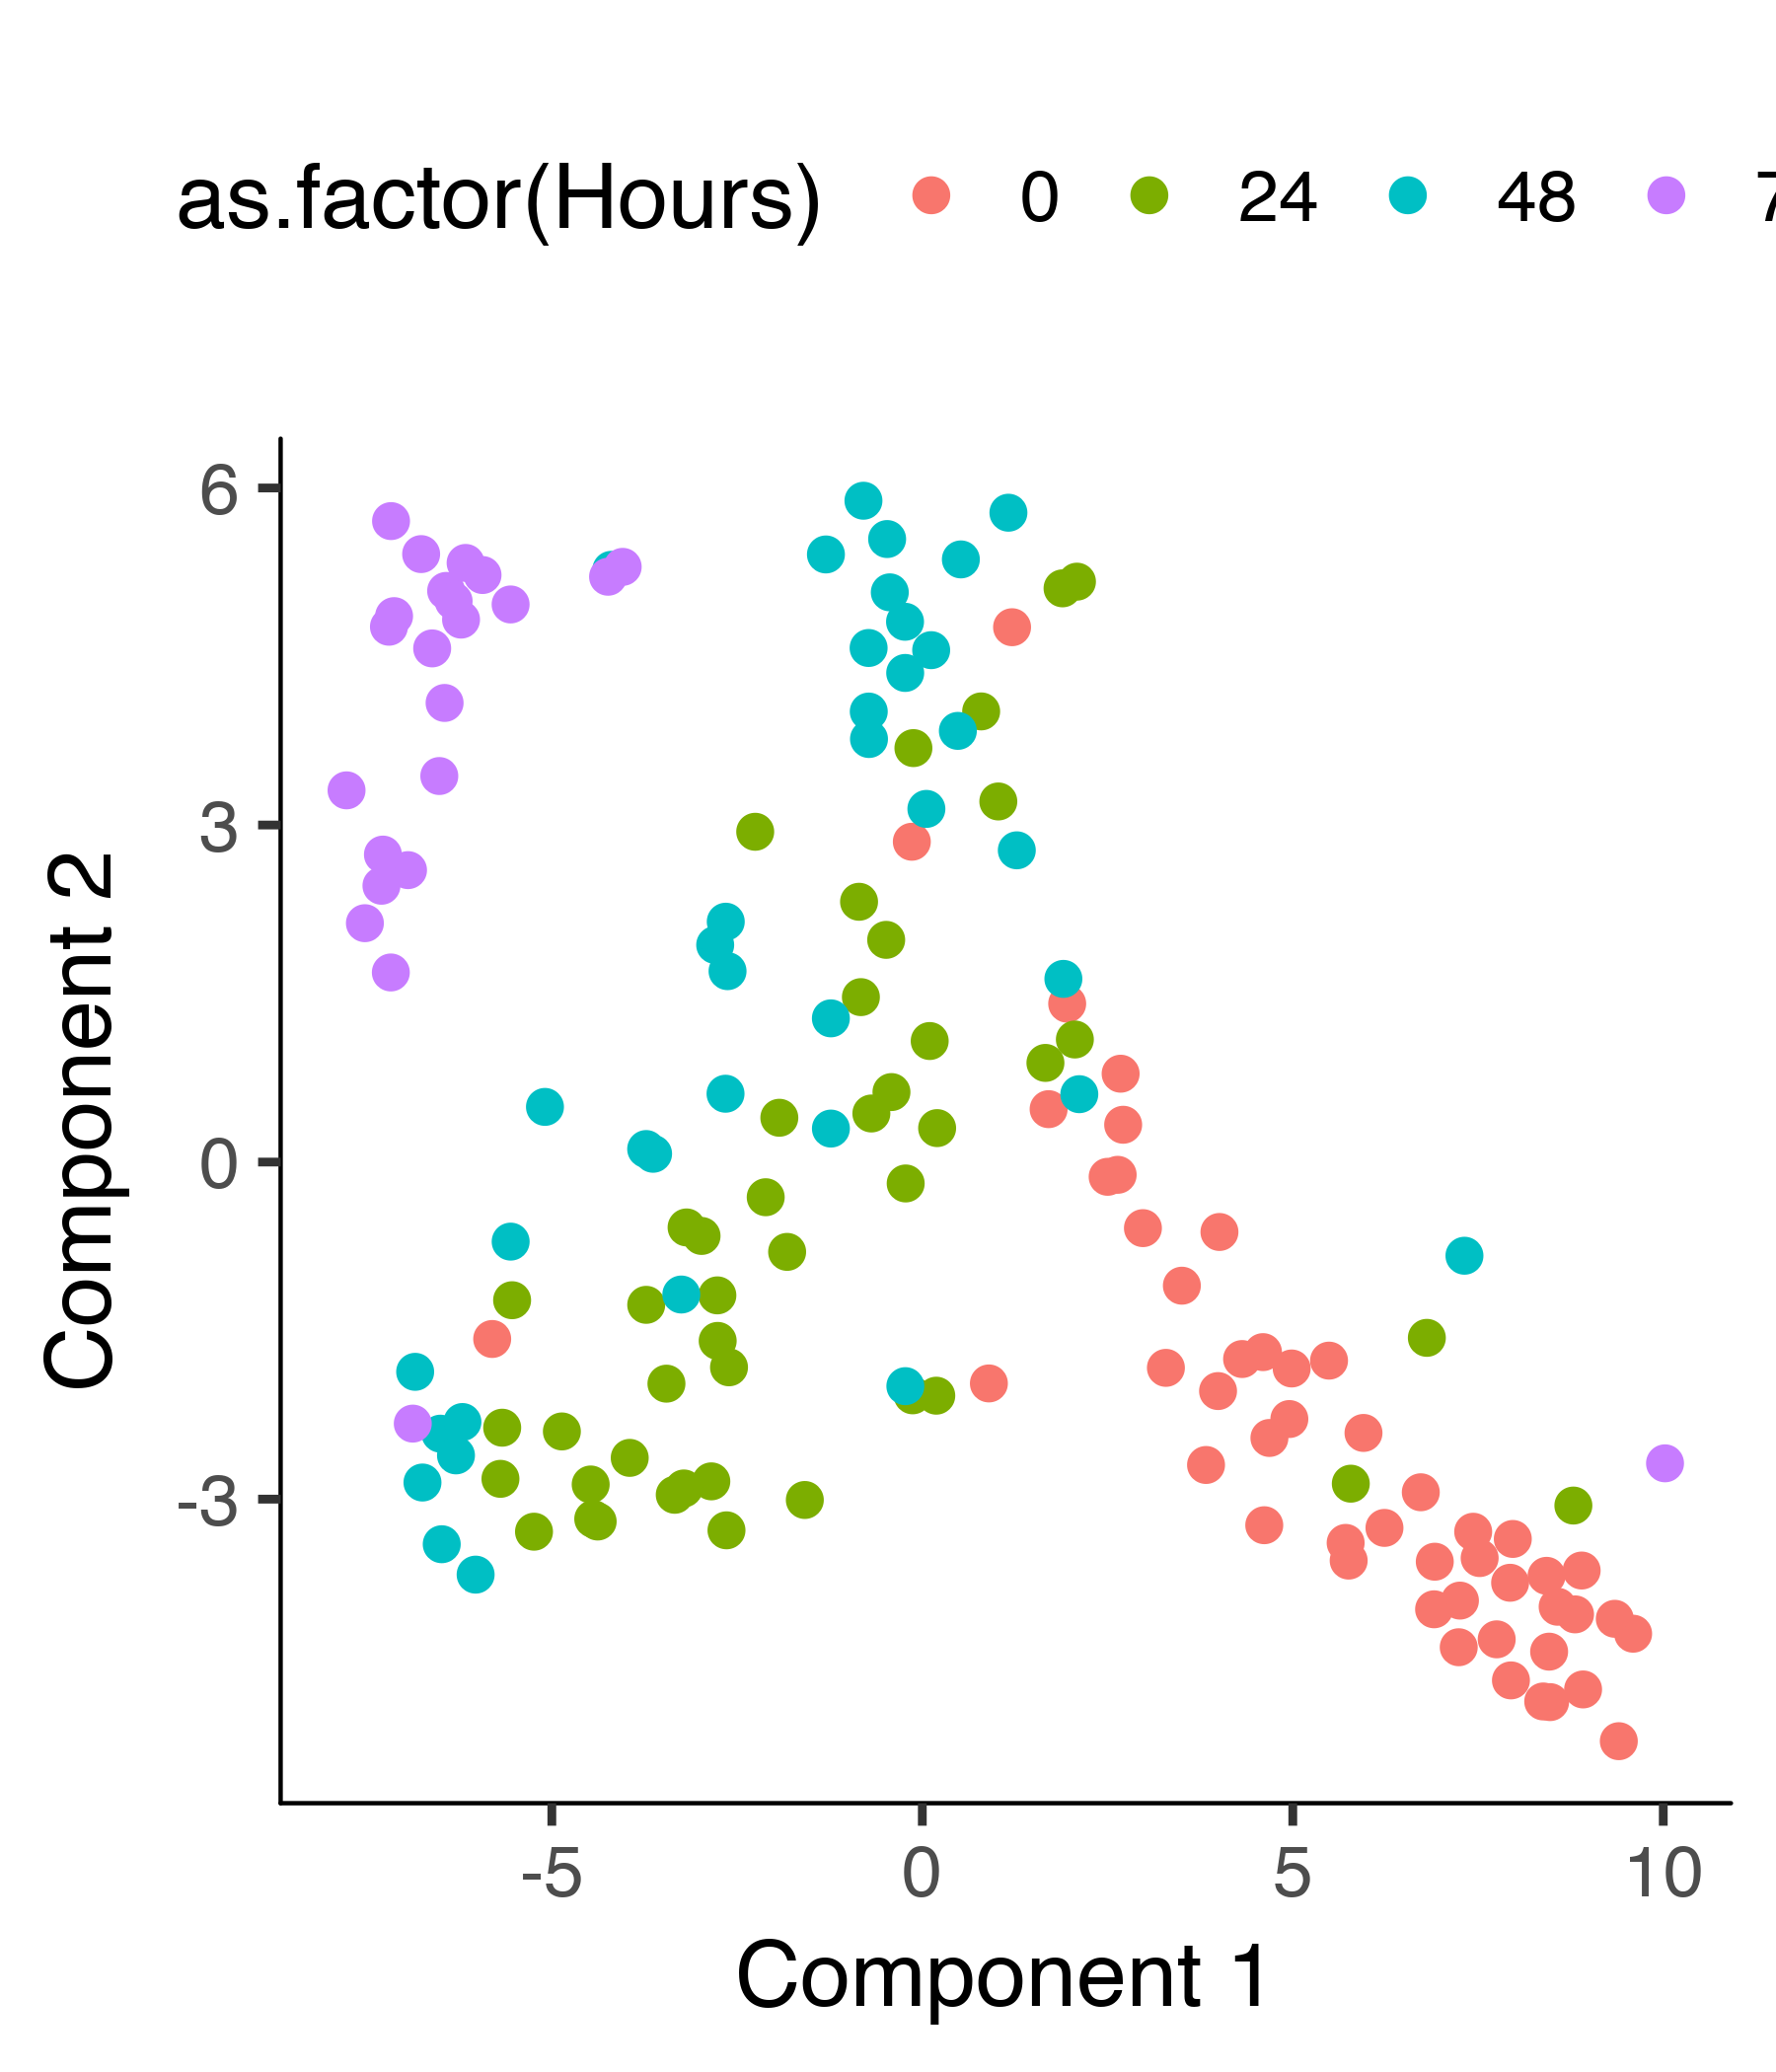
\includegraphics[width=\maxwidth]{figure/check_the_clustering_results-2} 

\end{knitrout}

We also provide the decision plot for users to check the $\rho, \delta$ for each cell and decide the threshold for defining the cell clusters. 
\begin{knitrout}
\definecolor{shadecolor}{rgb}{0.969, 0.969, 0.969}\color{fgcolor}\begin{kframe}
\begin{alltt}
\hlkwd{plot_rho_delta}\hlstd{(HSMM_myo,} \hlkwc{rho_threshold} \hlstd{=} \hlnum{2}\hlstd{,} \hlkwc{delta_threshold} \hlstd{=} \hlnum{4} \hlstd{)}
\end{alltt}
\end{kframe}

{\centering 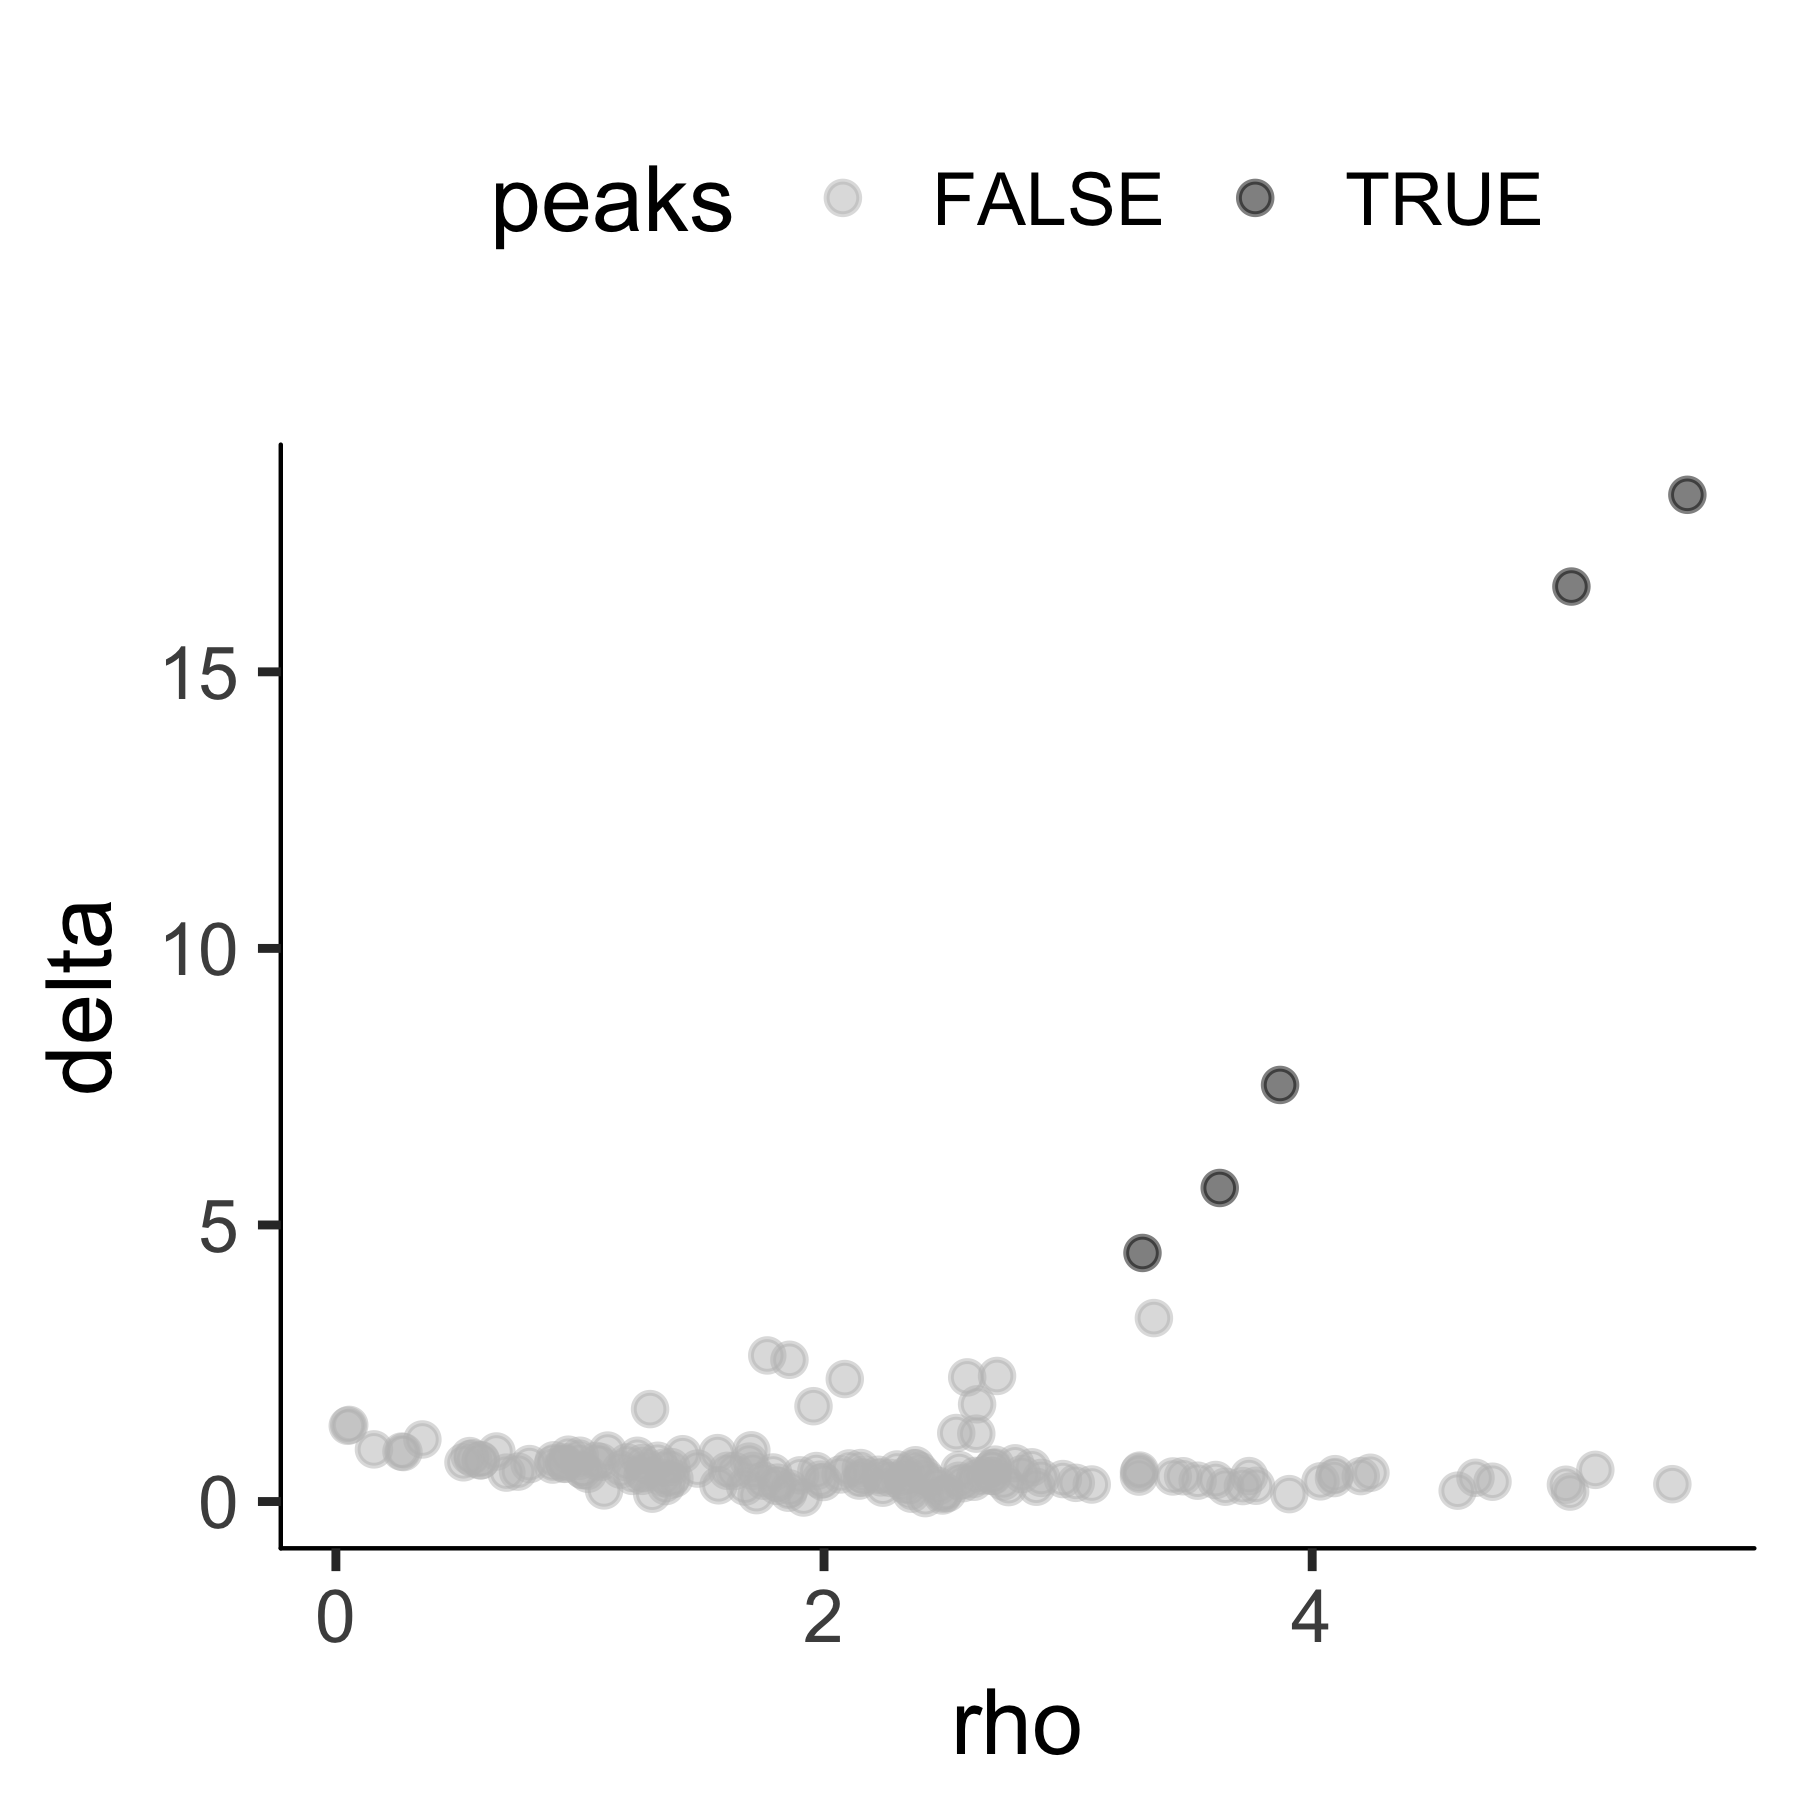
\includegraphics[width=\maxwidth]{figure/plot_rho_delta-1} 

}



\end{knitrout}

We could then re-run clustering based on the user defined threshold. To 
facilitate the computation, we can set \Rfunction(skip\_rho\_sigma = T) 
which enables us to skip the calculation of the $\rho, \sigma$.  
\begin{knitrout}
\definecolor{shadecolor}{rgb}{0.969, 0.969, 0.969}\color{fgcolor}\begin{kframe}
\begin{alltt}
\hlstd{HSMM_myo} \hlkwb{<-} \hlkwd{clusterCells}\hlstd{(HSMM_myo,}
                         \hlkwc{rho_threshold} \hlstd{=} \hlnum{2}\hlstd{,}
                         \hlkwc{delta_threshold} \hlstd{=} \hlnum{4}\hlstd{,}
                         \hlkwc{skip_rho_sigma} \hlstd{= T,}
                         \hlkwc{verbose} \hlstd{= F)}
\end{alltt}
\end{kframe}
\end{knitrout}

We can check the final clustering results as following: 
\begin{knitrout}
\definecolor{shadecolor}{rgb}{0.969, 0.969, 0.969}\color{fgcolor}\begin{kframe}
\begin{alltt}
\hlkwd{plot_cell_clusters}\hlstd{(HSMM_myo,} \hlkwc{color_by} \hlstd{=} \hlstr{'as.factor(Cluster)'}\hlstd{)}
\hlkwd{plot_cell_clusters}\hlstd{(HSMM_myo,} \hlkwc{color_by} \hlstd{=} \hlstr{'as.factor(Hours)'}\hlstd{)}
\end{alltt}
\end{kframe}
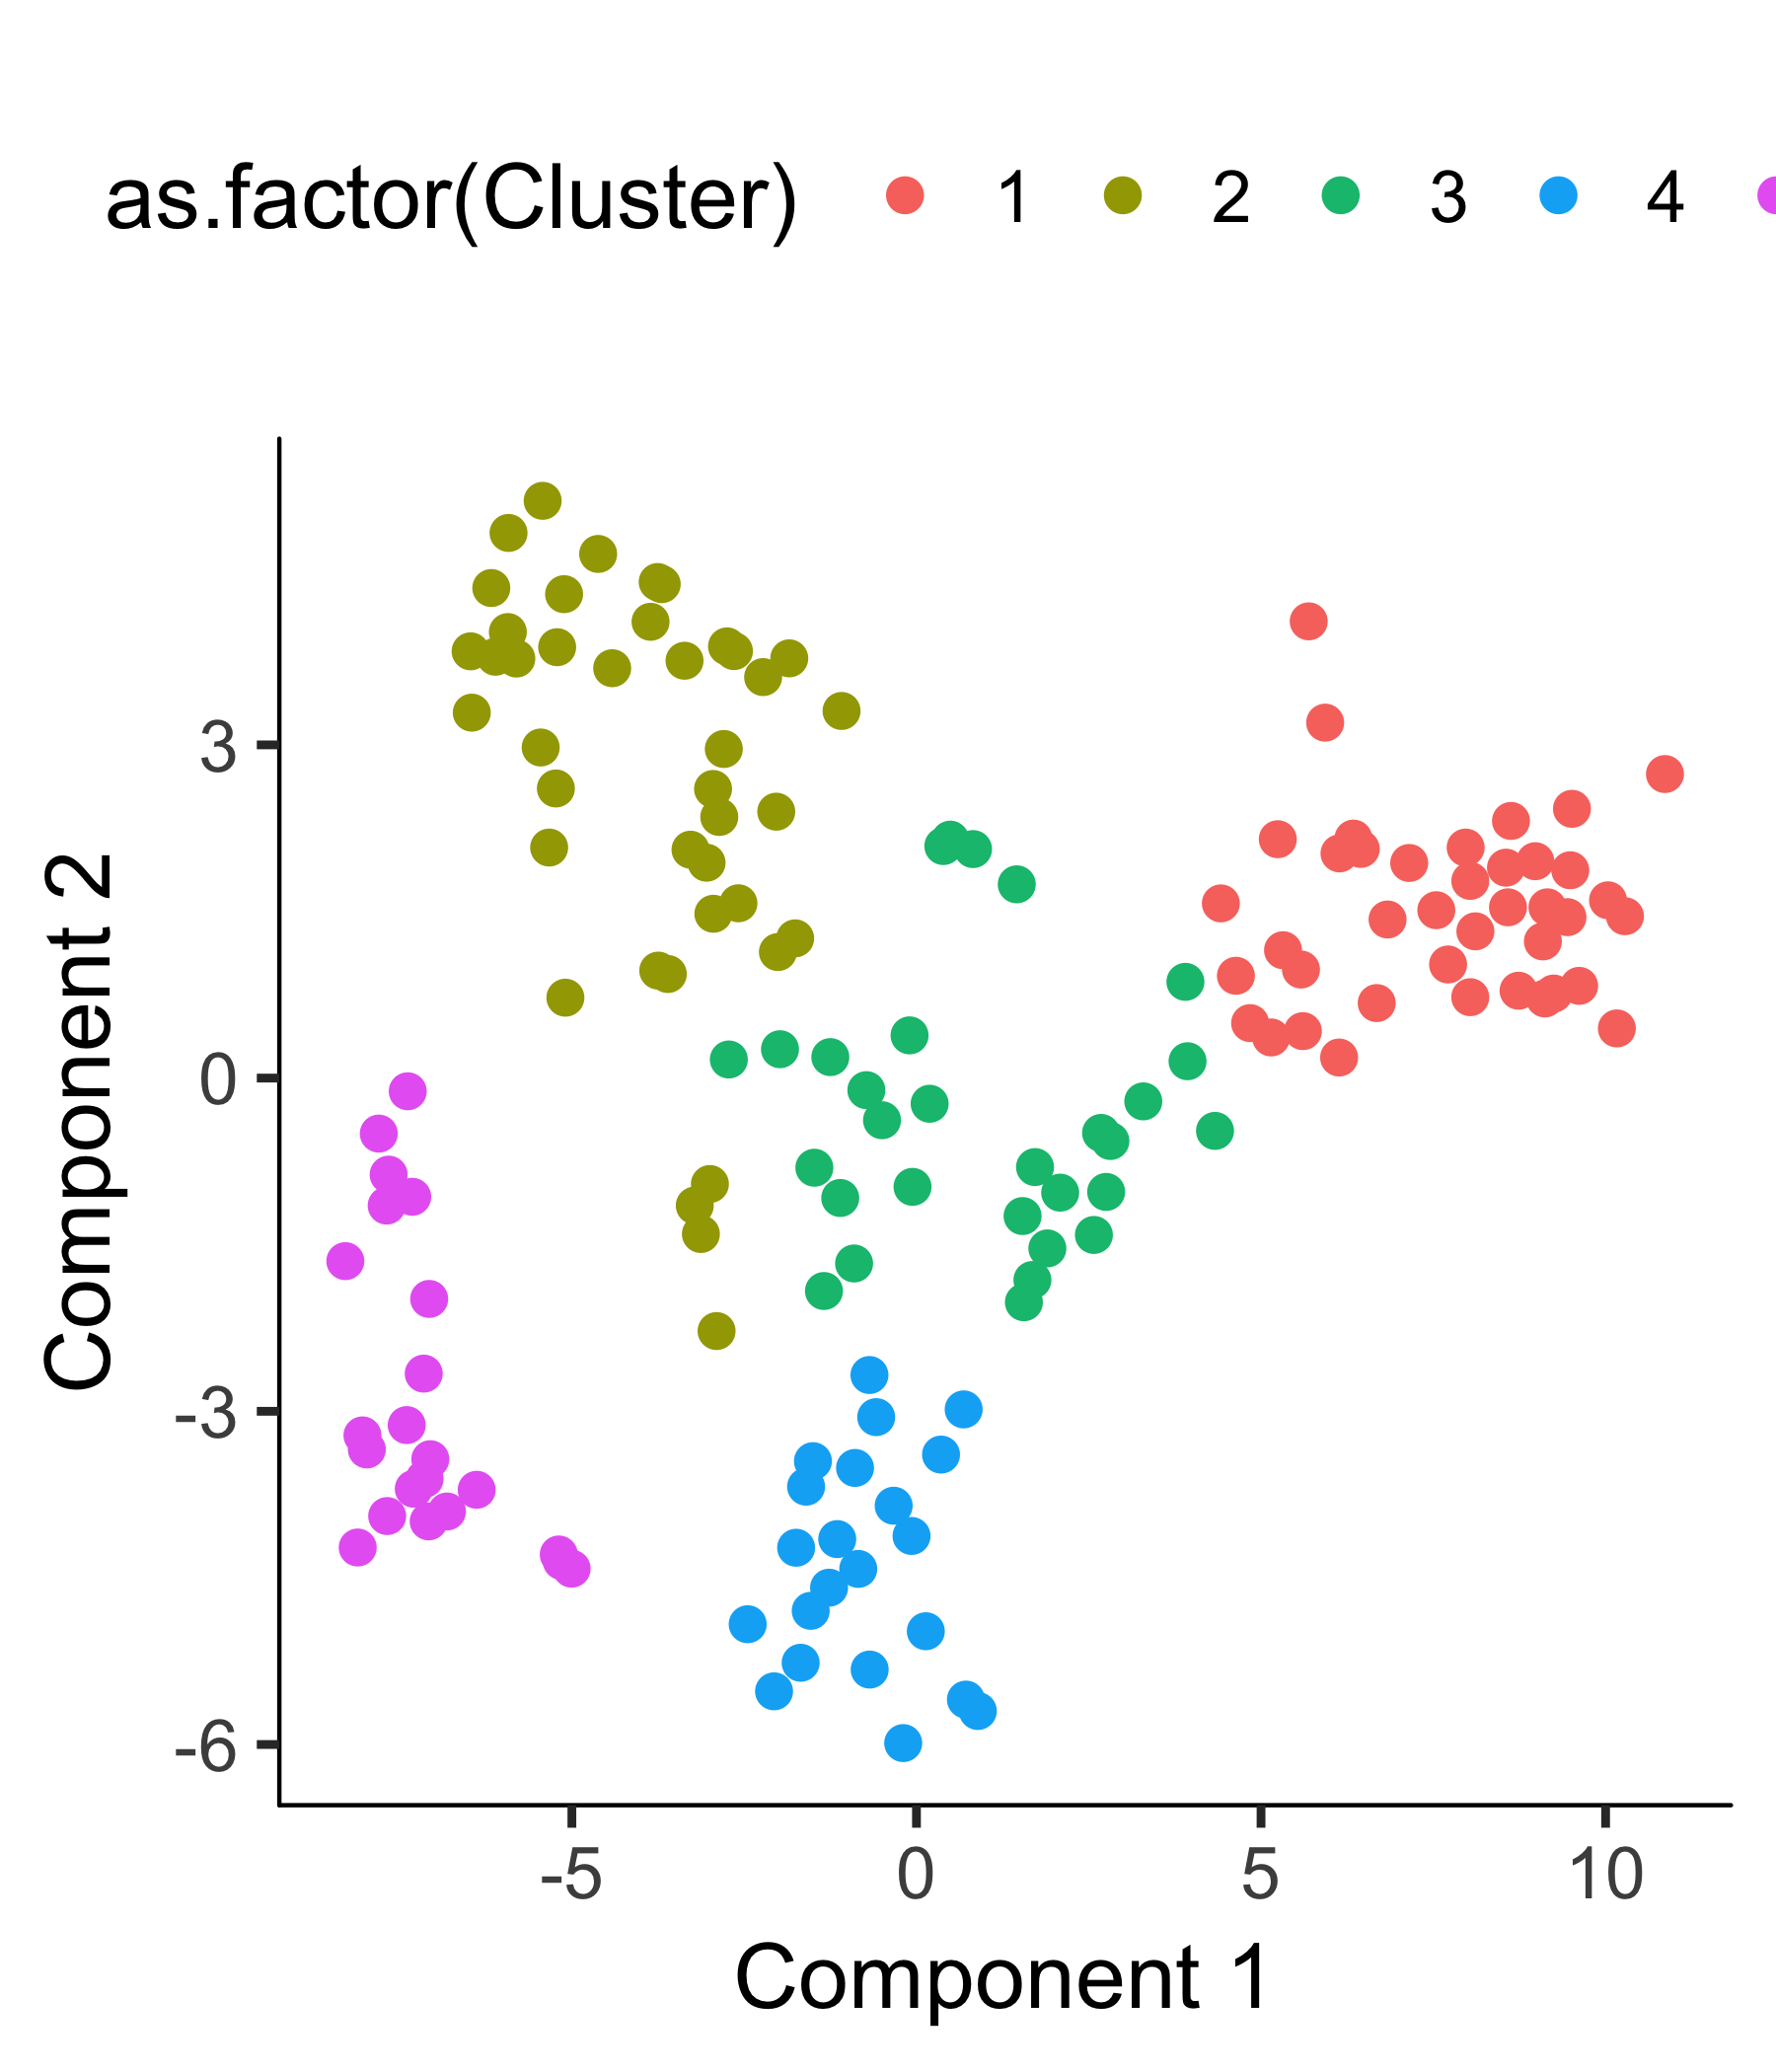
\includegraphics[width=\maxwidth]{figure/check_clustering_again-1} 
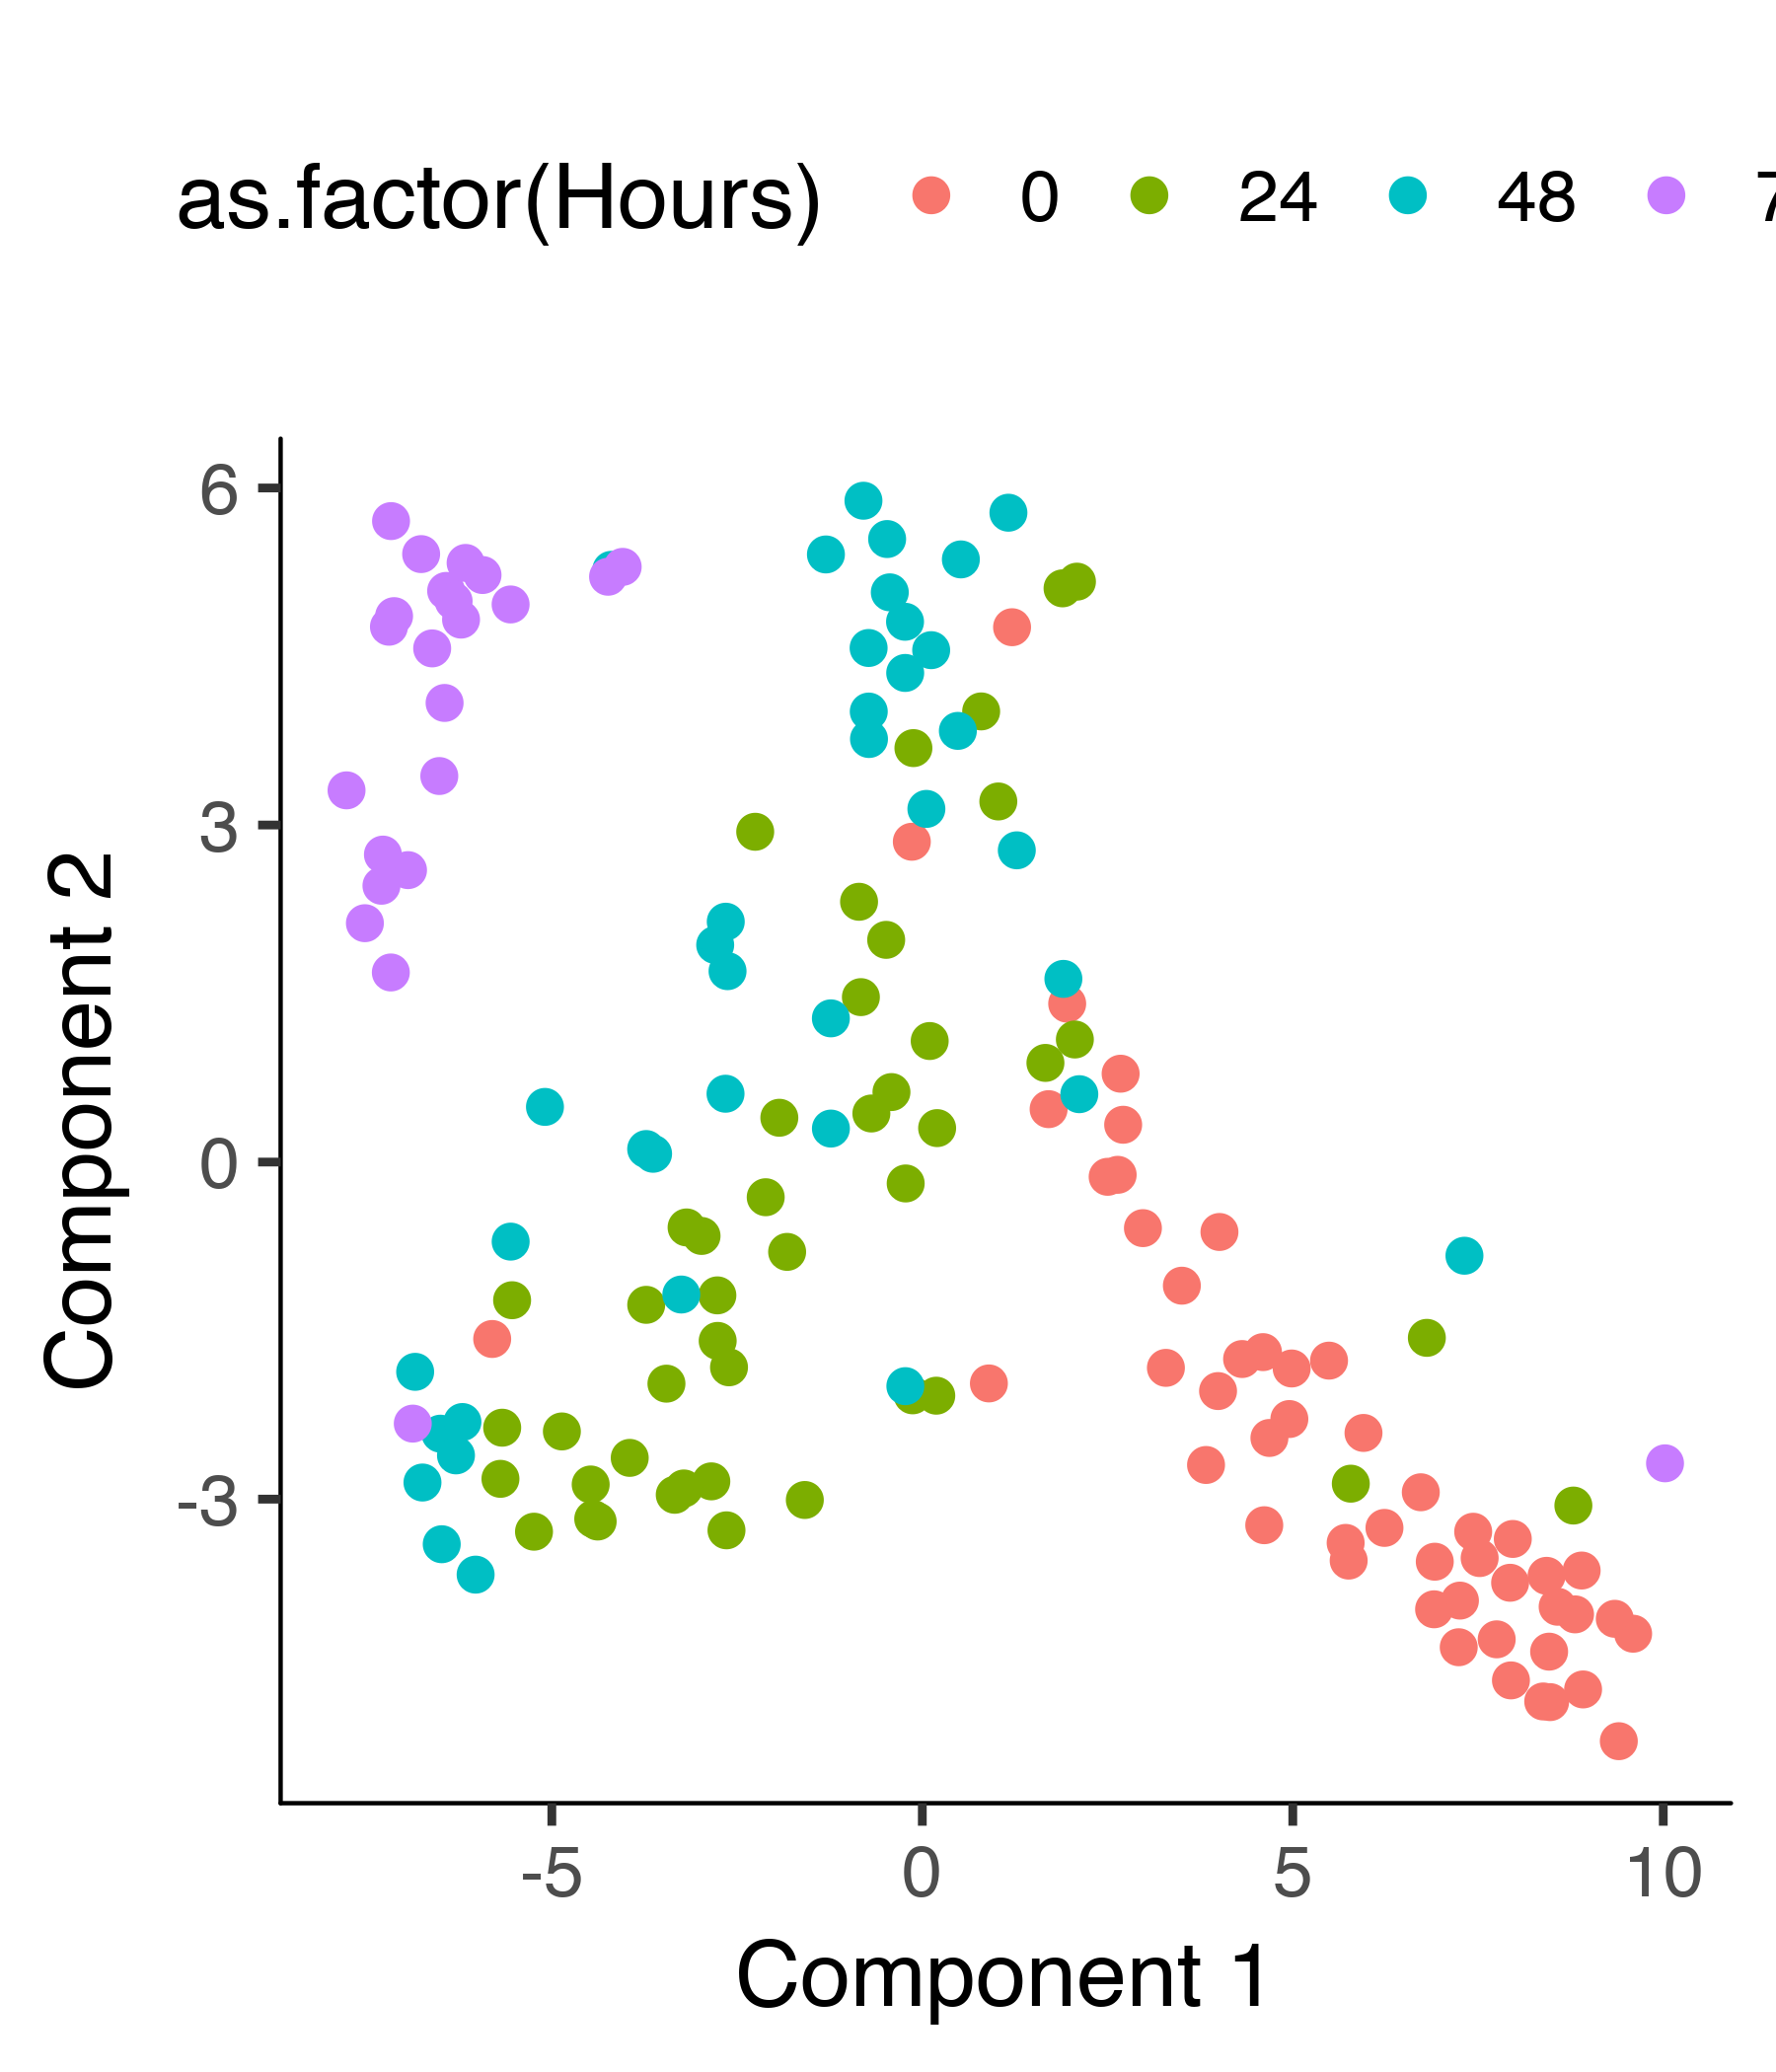
\includegraphics[width=\maxwidth]{figure/check_clustering_again-2} 

\end{knitrout}

After we confirm the clustering makes sense, we can then perform differential 
gene expression test as a way to extract the genes that distinguish them. 
\begin{knitrout}
\definecolor{shadecolor}{rgb}{0.969, 0.969, 0.969}\color{fgcolor}\begin{kframe}
\begin{alltt}
\hlstd{clustering_DEG_genes} \hlkwb{<-} \hlkwd{differentialGeneTest}\hlstd{(HSMM_myo[HSMM_expressed_genes,],}
                                             \hlkwc{fullModelFormulaStr} \hlstd{=} \hlstr{'~Cluster'}\hlstd{,}
                                             \hlkwc{cores} \hlstd{=} \hlkwd{detectCores}\hlstd{())}
\end{alltt}
\end{kframe}
\end{knitrout}



We will then select the top $1000$ significant genes as the ordering genes. 
\begin{knitrout}
\definecolor{shadecolor}{rgb}{0.969, 0.969, 0.969}\color{fgcolor}\begin{kframe}
\begin{alltt}
\hlstd{HSMM_ordering_genes} \hlkwb{<-} \hlkwd{row.names}\hlstd{(clustering_DEG_genes)[}\hlkwd{order}\hlstd{(clustering_DEG_genes}\hlopt{$}\hlstd{qval)][}\hlnum{1}\hlopt{:}\hlnum{1000}\hlstd{]}

\hlstd{HSMM_myo} \hlkwb{<-} \hlkwd{setOrderingFilter}\hlstd{(HSMM_myo,} \hlkwc{ordering_genes} \hlstd{= HSMM_ordering_genes)}
\hlstd{HSMM_myo} \hlkwb{<-} \hlkwd{reduceDimension}\hlstd{(HSMM_myo,} \hlkwc{method} \hlstd{=} \hlstr{'DDRTree'}\hlstd{)}
\hlstd{HSMM_myo} \hlkwb{<-} \hlkwd{orderCells}\hlstd{(HSMM_myo)}
\hlstd{HSMM_myo} \hlkwb{<-} \hlkwd{orderCells}\hlstd{(HSMM_myo,} \hlkwc{root_state}\hlstd{=}\hlkwd{GM_state}\hlstd{(HSMM_myo))}
\hlkwd{plot_cell_trajectory}\hlstd{(HSMM_myo,} \hlkwc{color_by}\hlstd{=}\hlstr{"Hours"}\hlstd{)}
\end{alltt}
\end{kframe}

{\centering 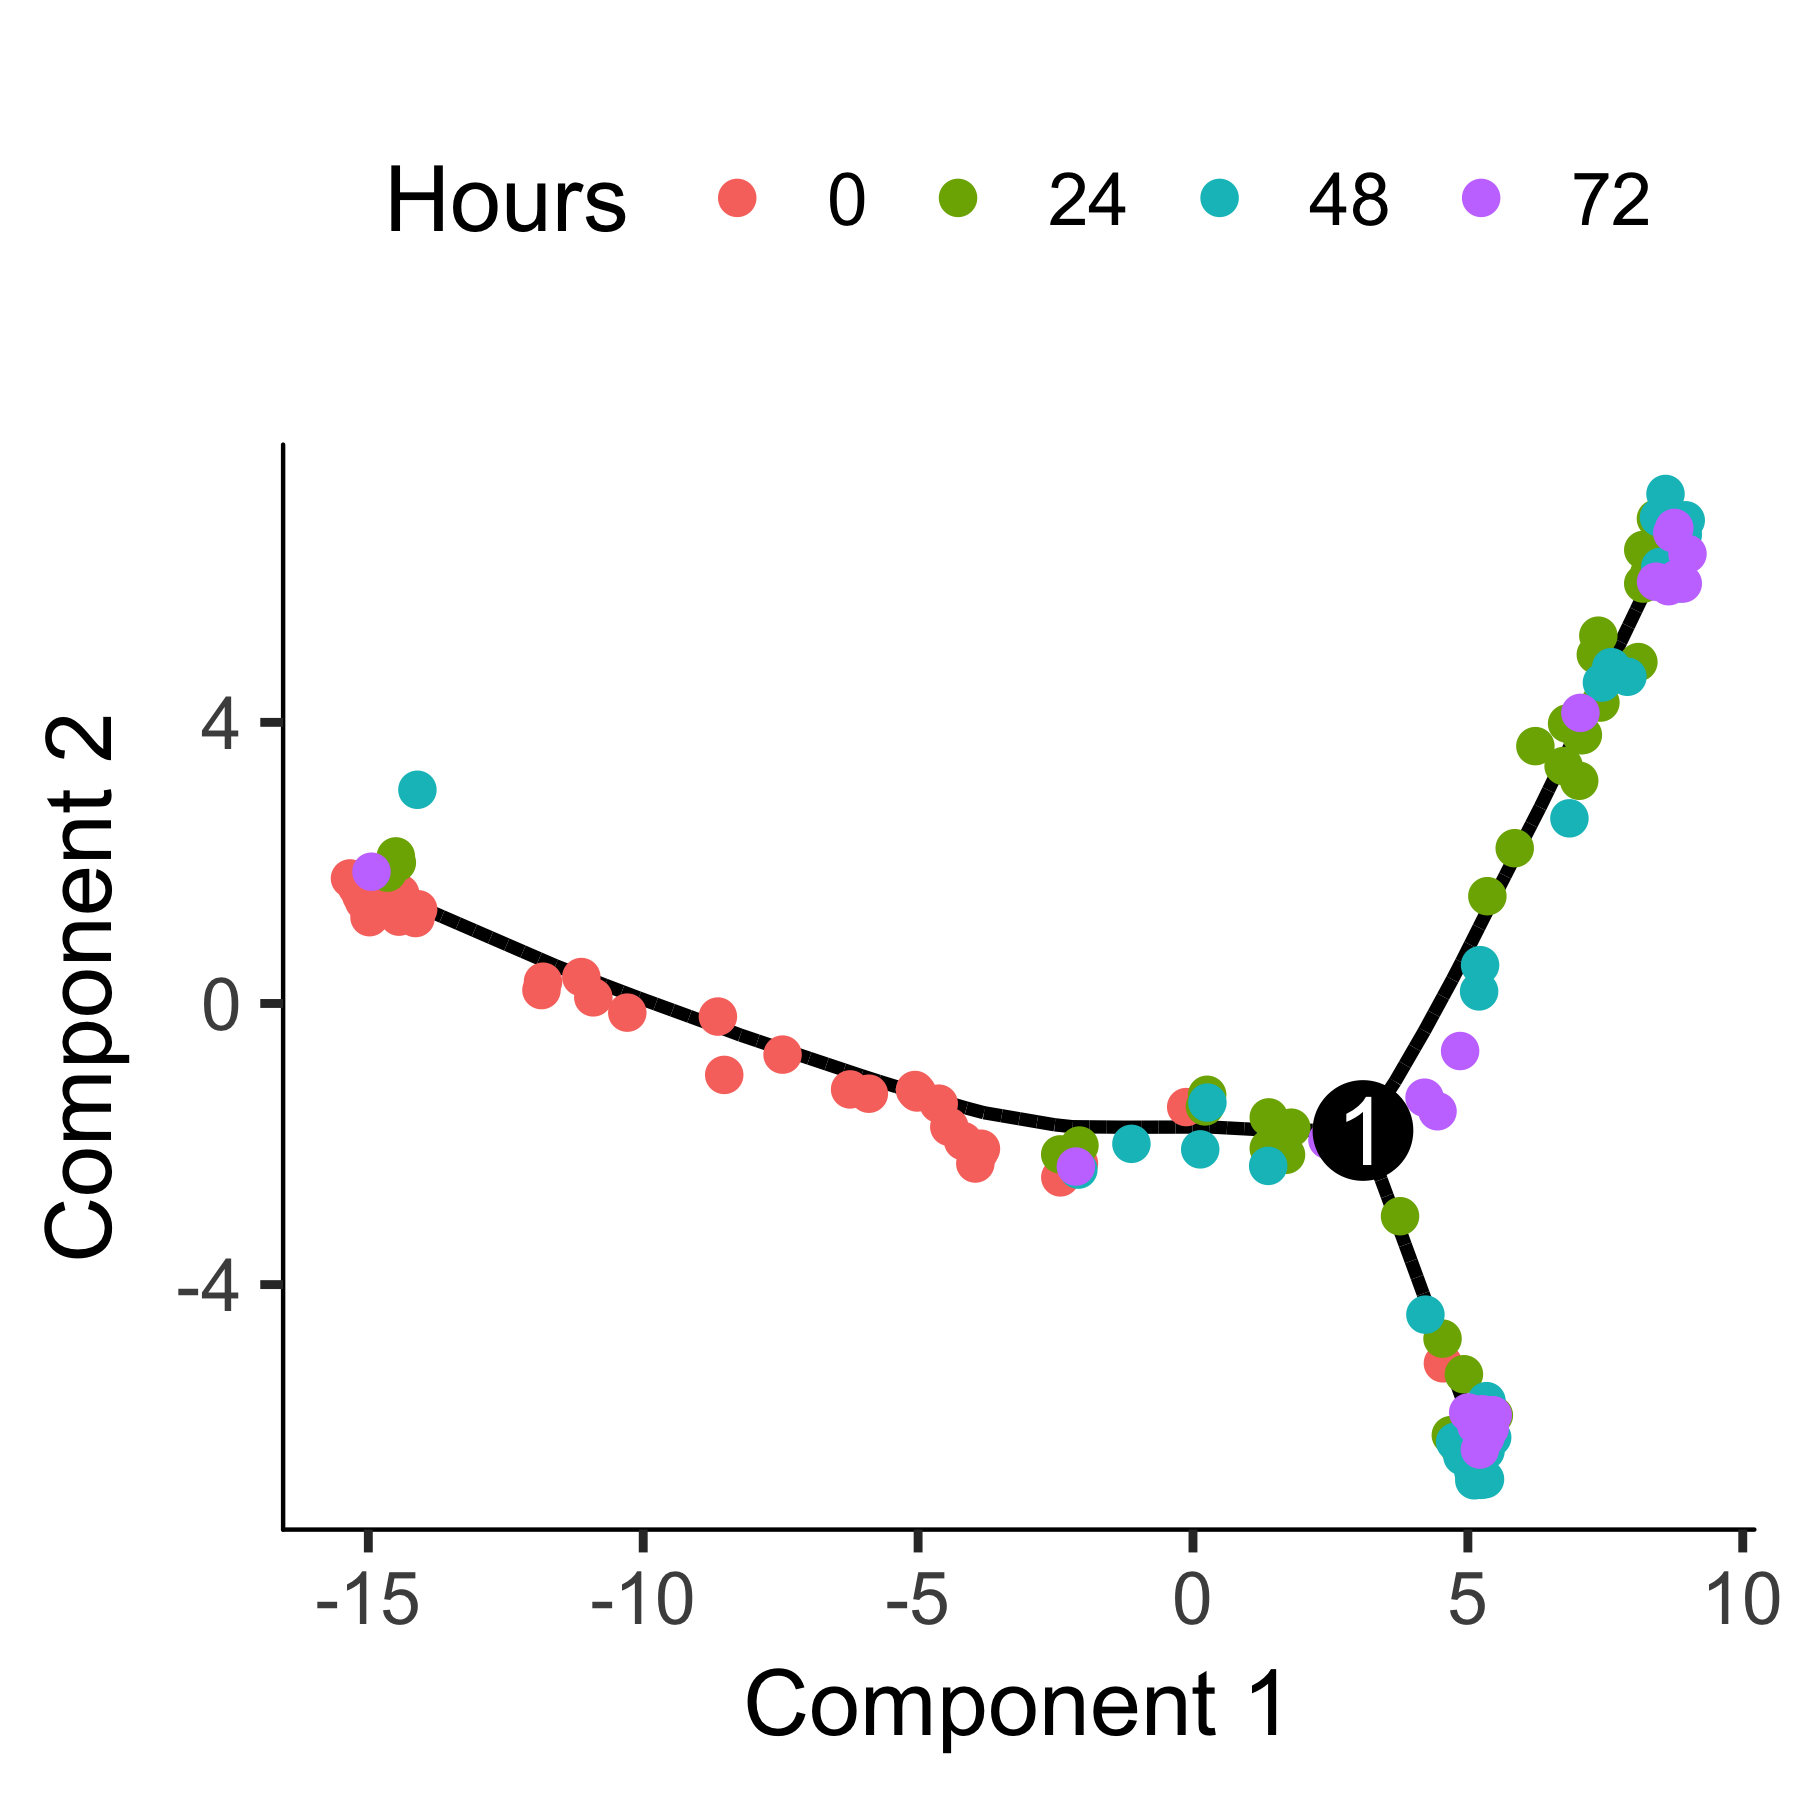
\includegraphics[width=\maxwidth]{figure/order_cells_dp_feature-1} 

}



\end{knitrout}

\subsection{Semi-supervised ordering with known marker genes}

Unsupervised ordering is desirable because it avoids introducing bias into the analysis. However, unsupervised machine learning will often fix on a strong feature of the data that's not the focus of your experiment. For example, where each cell is in the cell cycle has a major impact on the shape of the trajectory when you use unsupervised learning. But what if you wish to focus on cycle-independent effects in your biological process? Monocle's ``semi-supervised'' ordering mode can help you focus on the aspects of the process you're interested in.

Ordering your cells in a semi-supervised manner is very simple. You first define genes that mark progress using the \Robject{CellTypeHierchy} system, very similar to how we used it for cell type classification. Then, you use it to select ordering genes that co-vary with these markers. Finally, you order the cell based on these genes just as we do in unsupervised ordering. So the only difference between unsupervised and semi-supervised ordering is in which genes we use for ordering.

As we saw before, myoblasts begin differnentation by exiting the cell cycle and then proceed through a sequence of regulatory events that leads to expression of some key muscle-specific proteins needed for contraction. We can mark cycling cells with cyclin B2 (\emph{CCNB2}) and recognize myotubes as those cells expressed high levels of myosin heavy chain 3 (\emph{MYH3}).
\begin{knitrout}
\definecolor{shadecolor}{rgb}{0.969, 0.969, 0.969}\color{fgcolor}\begin{kframe}
\begin{alltt}
\hlstd{CCNB2_id} \hlkwb{<-} \hlkwd{row.names}\hlstd{(}\hlkwd{subset}\hlstd{(}\hlkwd{fData}\hlstd{(HSMM_myo), gene_short_name} \hlopt{==} \hlstr{"CCNB2"}\hlstd{))}
\hlstd{MYH3_id} \hlkwb{<-} \hlkwd{row.names}\hlstd{(}\hlkwd{subset}\hlstd{(}\hlkwd{fData}\hlstd{(HSMM_myo), gene_short_name} \hlopt{==} \hlstr{"MYH3"}\hlstd{))}

\hlstd{cth} \hlkwb{<-} \hlkwd{newCellTypeHierarchy}\hlstd{()}
\hlstd{cth} \hlkwb{<-} \hlkwd{addCellType}\hlstd{(cth,} \hlstr{"Cycling myoblast"}\hlstd{,} \hlkwc{classify_func}\hlstd{=}\hlkwa{function}\hlstd{(}\hlkwc{x}\hlstd{) \{x[CCNB2_id,]} \hlopt{>=} \hlnum{1}\hlstd{\})}
\hlstd{cth} \hlkwb{<-} \hlkwd{addCellType}\hlstd{(cth,} \hlstr{"Myotube"}\hlstd{,} \hlkwc{classify_func}\hlstd{=}\hlkwa{function}\hlstd{(}\hlkwc{x}\hlstd{) \{x[MYH3_id,]} \hlopt{>=}\hlnum{1}\hlstd{\})}
\hlstd{cth} \hlkwb{<-} \hlkwd{addCellType}\hlstd{(cth,} \hlstr{"Reserve cell"}\hlstd{,} \hlkwc{classify_func}\hlstd{=}\hlkwa{function}\hlstd{(}\hlkwc{x}\hlstd{) \{x[MYH3_id,]} \hlopt{==} \hlnum{0} \hlopt{&} \hlstd{x[CCNB2_id,]} \hlopt{==} \hlnum{0}\hlstd{\})}
\hlstd{HSMM_myo} \hlkwb{<-} \hlkwd{classifyCells}\hlstd{(HSMM_myo, cth)}
\end{alltt}
\end{kframe}
\end{knitrout}

Now we select the set of genes that co-vary (in either direction) with these two ``bellweather'' genes:
\begin{knitrout}
\definecolor{shadecolor}{rgb}{0.969, 0.969, 0.969}\color{fgcolor}\begin{kframe}
\begin{alltt}
\hlstd{marker_diff} \hlkwb{<-} \hlkwd{markerDiffTable}\hlstd{(HSMM_myo[HSMM_expressed_genes,],}
                               \hlstd{cth,}
                               \hlkwc{cores}\hlstd{=}\hlkwd{detectCores}\hlstd{())}
\hlcom{#semisup_clustering_genes <- row.names(subset(marker_diff, qval < 0.05))}
\hlstd{semisup_clustering_genes} \hlkwb{<-} \hlkwd{row.names}\hlstd{(marker_diff)[}\hlkwd{order}\hlstd{(marker_diff}\hlopt{$}\hlstd{qval)][}\hlnum{1}\hlopt{:}\hlnum{1000}\hlstd{]}
\end{alltt}
\end{kframe}
\end{knitrout}



Using the top 1000 genes for ordering produces a trajectory that's highly similar to the one we obtained with unsupervised methods, but it's a little ``cleaner''.
\begin{knitrout}
\definecolor{shadecolor}{rgb}{0.969, 0.969, 0.969}\color{fgcolor}\begin{kframe}
\begin{alltt}
\hlstd{HSMM_myo} \hlkwb{<-} \hlkwd{setOrderingFilter}\hlstd{(HSMM_myo, semisup_clustering_genes)}
\hlcom{#plot_ordering_genes(HSMM_myo)}
\hlstd{HSMM_myo} \hlkwb{<-} \hlkwd{reduceDimension}\hlstd{(HSMM_myo,} \hlkwc{max_components}\hlstd{=}\hlnum{2}\hlstd{,} \hlkwc{method} \hlstd{=} \hlstr{'DDRTree'}\hlstd{,} \hlkwc{norm_method} \hlstd{=} \hlstr{'log'}\hlstd{)}
\hlstd{HSMM_myo} \hlkwb{<-} \hlkwd{orderCells}\hlstd{(HSMM_myo)}
\hlstd{HSMM_myo} \hlkwb{<-} \hlkwd{orderCells}\hlstd{(HSMM_myo,} \hlkwc{root_state}\hlstd{=}\hlkwd{GM_state}\hlstd{(HSMM_myo))}
\hlkwd{plot_cell_trajectory}\hlstd{(HSMM_myo,} \hlkwc{color_by}\hlstd{=}\hlstr{"CellType"}\hlstd{)} \hlopt{+} \hlkwd{theme}\hlstd{(}\hlkwc{legend.position}\hlstd{=}\hlstr{"right"}\hlstd{)}
\end{alltt}
\end{kframe}

{\centering 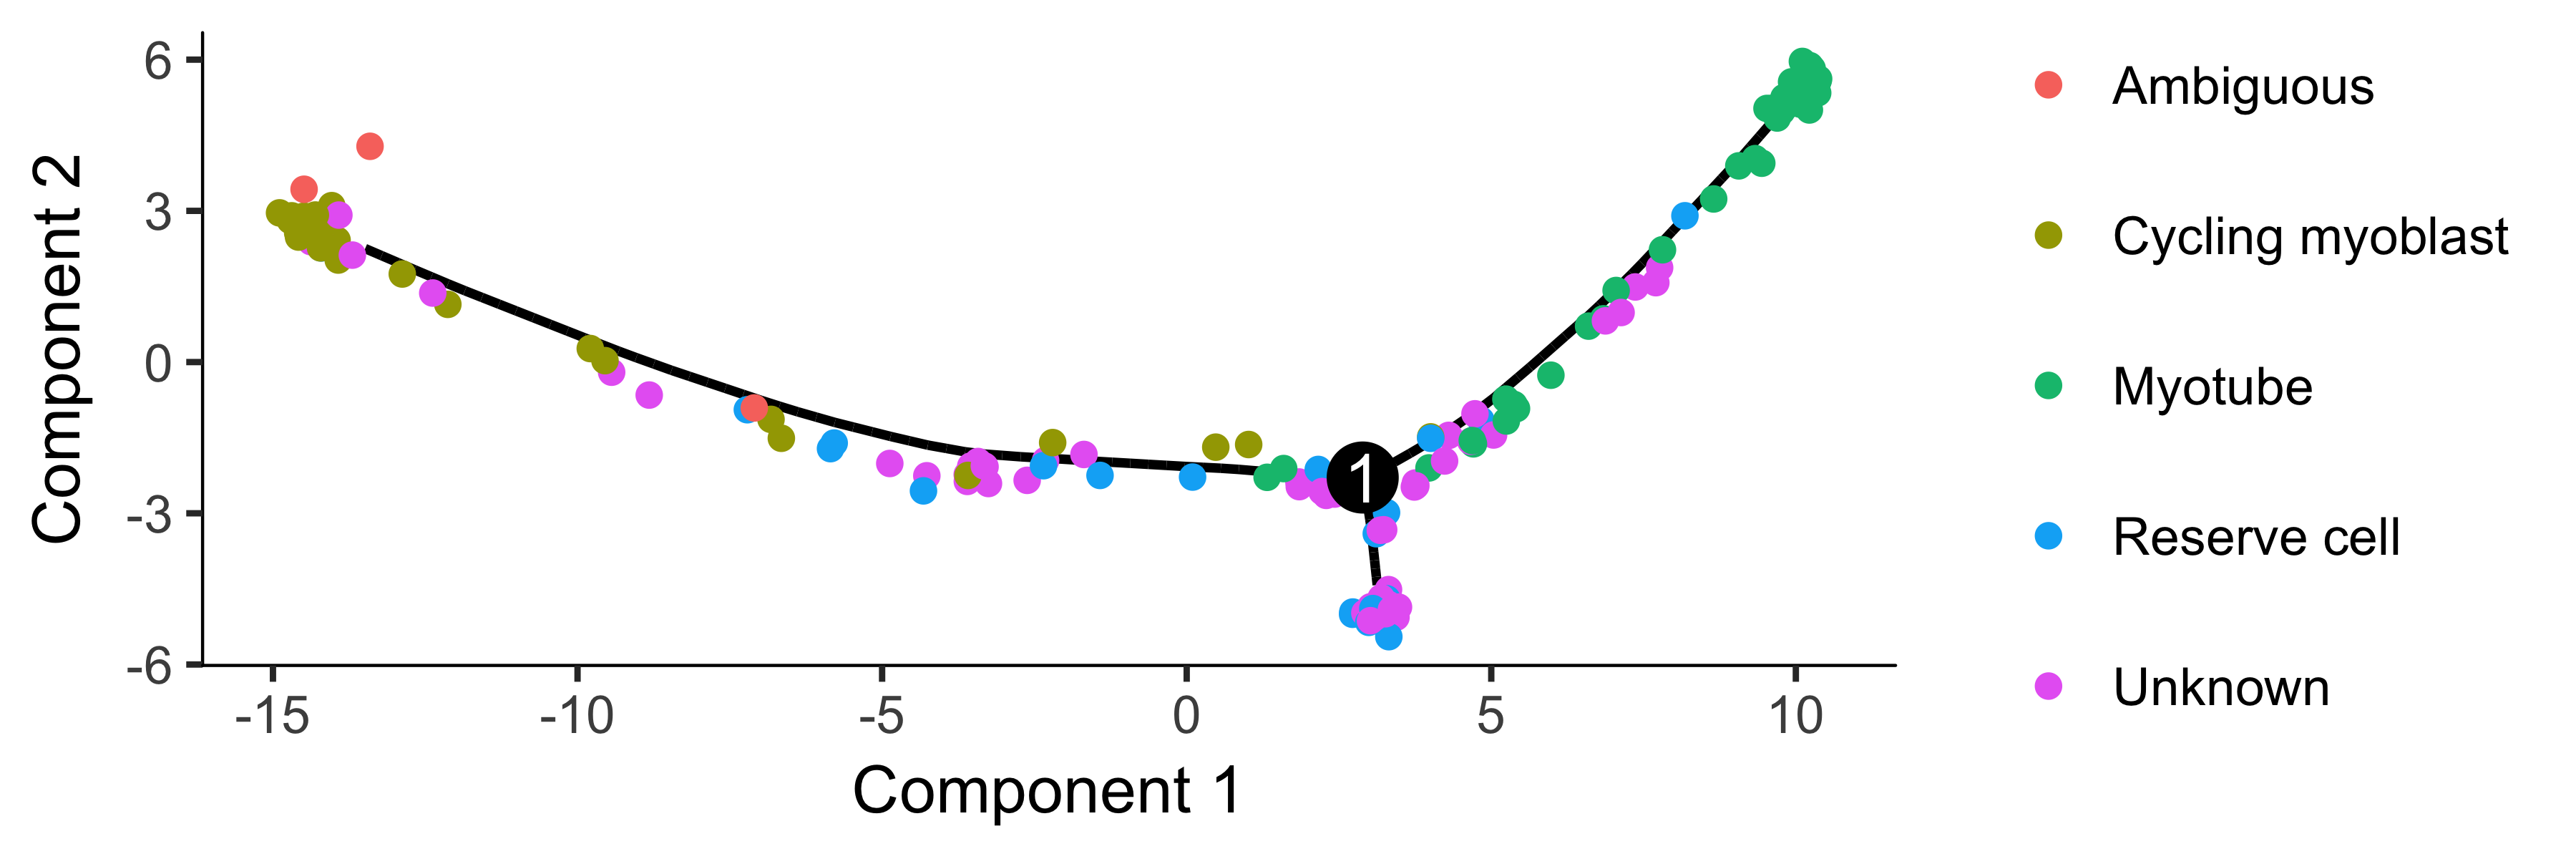
\includegraphics[width=\maxwidth]{figure/semi_sup_ordering_trajectory-1} 

}



\end{knitrout}

To confirm that the ordering is correct, we can select a couple of markers of 
myogenic progress. In this experiment, one of the branches corresponds to cells
that successfully fuse to form myotubes, and the other to those that fail to 
fully differentiate. We'll exclude the latter for now, but you can learn more 
about tools for dealing with branched trajectories in section \ref{BEAM_trajectory}.

\begin{knitrout}
\definecolor{shadecolor}{rgb}{0.969, 0.969, 0.969}\color{fgcolor}\begin{kframe}
\begin{alltt}
\hlstd{HSMM_filtered} \hlkwb{<-} \hlstd{HSMM_myo[HSMM_expressed_genes,]}

\hlstd{my_genes} \hlkwb{<-} \hlkwd{row.names}\hlstd{(}\hlkwd{subset}\hlstd{(}\hlkwd{fData}\hlstd{(HSMM_filtered),}
                             \hlstd{gene_short_name} \hlopt \hlkwd{c}\hlstd{(}\hlstr{"CDK1"}\hlstd{,} \hlstr{"MEF2C"}\hlstd{,} \hlstr{"MYH3"}\hlstd{)))}

\hlstd{cds_subset} \hlkwb{<-} \hlstd{HSMM_filtered[my_genes,]}
\hlkwd{plot_genes_branched_pseudotime}\hlstd{(cds_subset,}
                               \hlkwc{branch_point}\hlstd{=}\hlnum{1}\hlstd{,}
                               \hlkwc{color_by}\hlstd{=}\hlstr{"Hours"}\hlstd{,}
                               \hlkwc{ncol}\hlstd{=}\hlnum{1}\hlstd{)}
\end{alltt}
\end{kframe}

{\centering 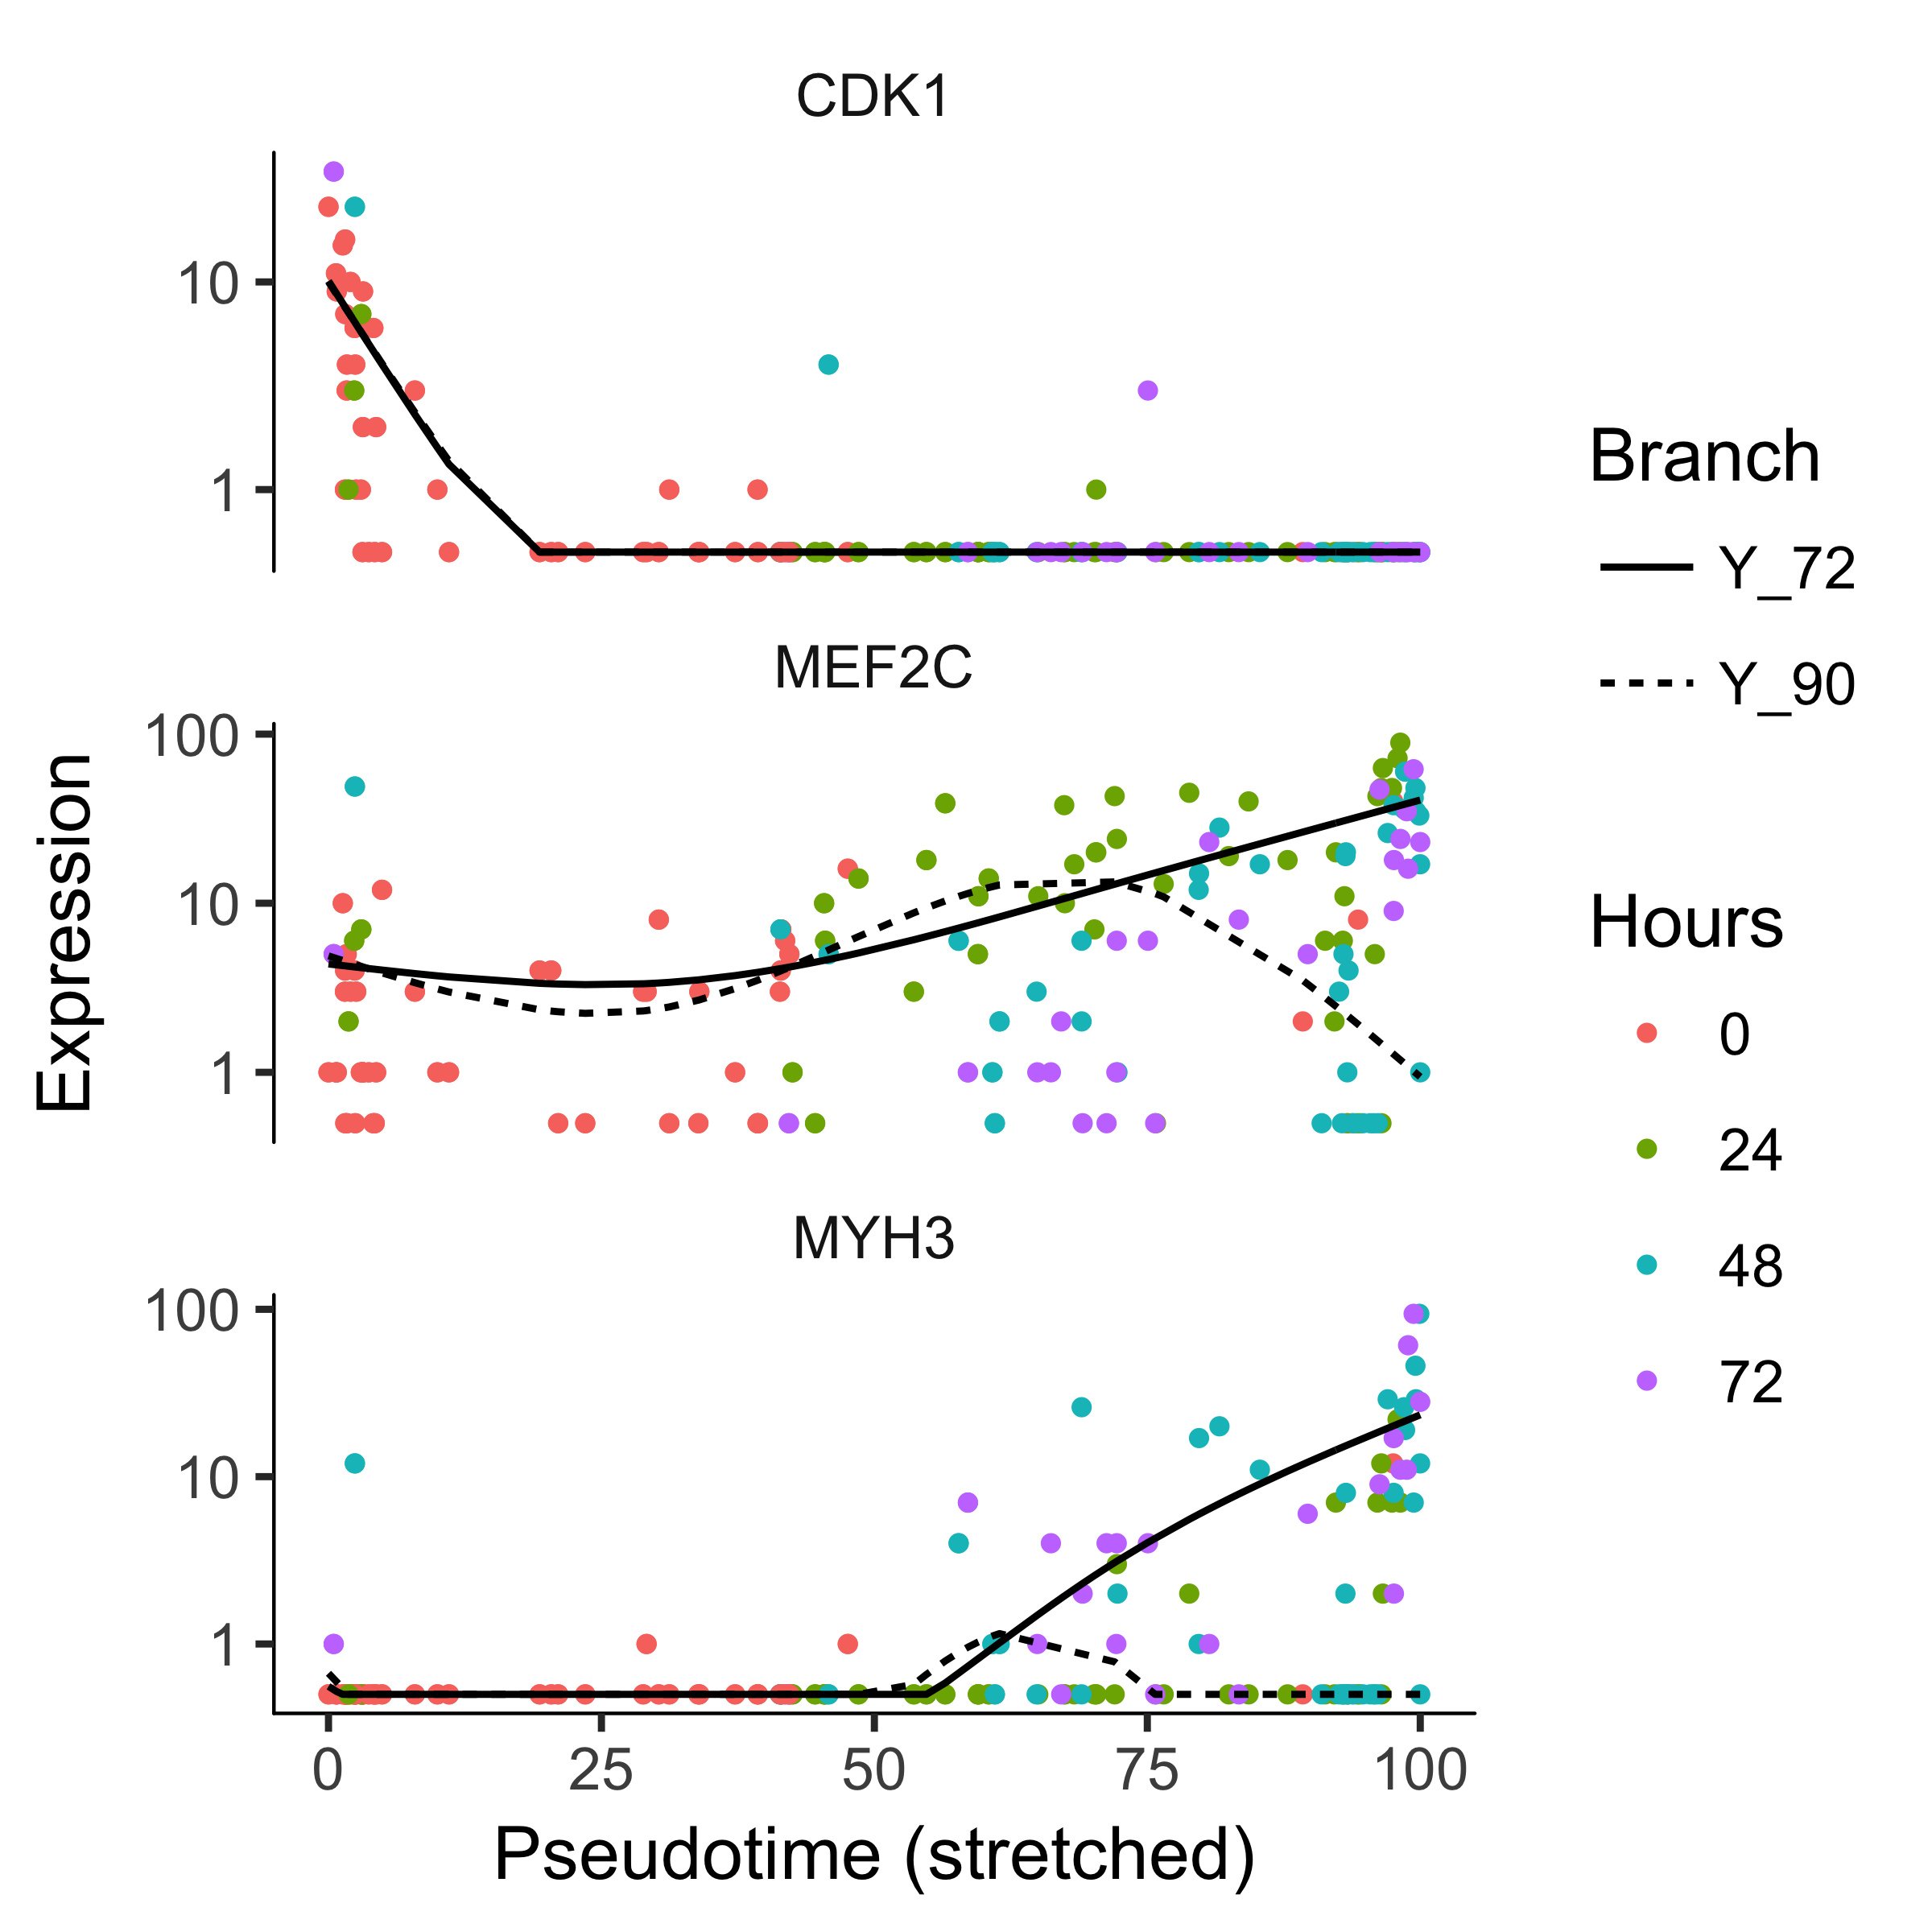
\includegraphics[width=\maxwidth]{figure/semi_sup_ordering_genes_in_pseudotime-1} 

}



\end{knitrout}


% \subsection{Learning trajectories using other dimension reduction methods}
% Recently, a few groups have applied some non-linear dimension reduction methods, including diffusion maps, LLE (local linear embedding), etc., to facilitate trajectory reconstruction. Monocle 2 provides a very convinient way for users who are interested in them to seamlessly integrate RGE with those methods by simplying passing a dimension reduction method to the argument \Robject{initial\_method} in \Rfunction{reduceDimension}. For example, we can use the nice package destiny$ , from the Fabian group, to perform the diffusion map dimension reduction and a function as following to the \Rfunction{reduceDimension} function.
% 
% <<dpt_dm, include=TRUE, eval=TRUE, fig.width = 3, fig.height = 3.5, warning=FALSE, fig.align="center">>=
% #run L1 graph
% library(destiny)
% run_dpt <- function(data, branching = T, norm_method = 'log', verbose = F){
%   data <- t(data) 
%   data <- data[!duplicated(data), ]
%   dm <- DiffusionMap(as.matrix(data))
%   return(dm@eigenvectors)
% }
% @ %def 
% 
% Result after applying DDRTree: 
% <<run_DDRTree_dpt, include=TRUE, eval=TRUE, fig.width = 3, fig.height = 3.5, warning=FALSE, fig.align="center">>=
% #run DDRTree
% lung <- reduceDimension(lung, norm_method="log", pseudo_expr = 1, reduction_method = 'DDRTree', initial_method = run_dpt) #
% lung <- orderCells(lung)
% plot_cell_trajectory(lung, color_by="Time")
% @ %def 

\section{Differential expression analysis}

Differential gene expression analysis is a common task in RNA-Seq experiments.  Monocle can help you find genes that are differentially expressed between groups of cells and assesses the statistical signficance of those changes. These comparisons require that you have a way to collect your cells into two or more groups.  These groups are defined by columns in the \Robject{phenoData} table of each \Robject{CellDataSet}.  Monocle will assess the signficance of each gene's expression level across the different groups of cells.

\subsection{Basic differential analysis}

Performing differential expression analysis on all genes in the human genome can take a substantial amount of time. For a dataset as large as the myoblast data from \cite{TRAPNELL_CACCHIARELLI}, which contains several hundred cells, the analysis can take several hours on a single CPU. Let's select a small set of genes that we know are important in myogenesis to demonstrate Monocle's capabilities: 
\begin{knitrout}
\definecolor{shadecolor}{rgb}{0.969, 0.969, 0.969}\color{fgcolor}\begin{kframe}
\begin{alltt}
\hlstd{marker_genes} \hlkwb{<-} \hlkwd{row.names}\hlstd{(}\hlkwd{subset}\hlstd{(}\hlkwd{fData}\hlstd{(HSMM_myo),}
                                 \hlstd{gene_short_name} \hlopt \hlkwd{c}\hlstd{(}\hlstr{"MEF2C"}\hlstd{,} \hlstr{"MEF2D"}\hlstd{,} \hlstr{"MYF5"}\hlstd{,}
                                                        \hlstr{"ANPEP"}\hlstd{,} \hlstr{"PDGFRA"}\hlstd{,}\hlstr{"MYOG"}\hlstd{,}
                                                        \hlstr{"TPM1"}\hlstd{,}  \hlstr{"TPM2"}\hlstd{,}  \hlstr{"MYH2"}\hlstd{,}
                                                        \hlstr{"MYH3"}\hlstd{,}  \hlstr{"NCAM1"}\hlstd{,} \hlstr{"TNNT1"}\hlstd{,}
                                                        \hlstr{"TNNT2"}\hlstd{,} \hlstr{"TNNC1"}\hlstd{,} \hlstr{"CDK1"}\hlstd{,}
                                                        \hlstr{"CDK2"}\hlstd{,}  \hlstr{"CCNB1"}\hlstd{,} \hlstr{"CCNB2"}\hlstd{,}
                                                        \hlstr{"CCND1"}\hlstd{,} \hlstr{"CCNA1"}\hlstd{,} \hlstr{"ID1"}\hlstd{)))}
\end{alltt}
\end{kframe}
\end{knitrout}

In the myoblast data, the cells collected at the outset of the experiment were cultured in ``growth medium'' (GM) to prevent them from differentiating.  After they were harvested, the rest of the cells were switched over to ``differentiation medium'' (DM) to promote differentiation. Let's have monocle find which of the genes above are affected by this switch:
\begin{knitrout}
\definecolor{shadecolor}{rgb}{0.969, 0.969, 0.969}\color{fgcolor}\begin{kframe}
\begin{alltt}
\hlstd{diff_test_res} \hlkwb{<-} \hlkwd{differentialGeneTest}\hlstd{(HSMM_myo[marker_genes,],}
                                      \hlkwc{fullModelFormulaStr}\hlstd{=}\hlstr{"~Media"}\hlstd{,}
                                      \hlkwc{cores} \hlstd{=} \hlkwd{detectCores}\hlstd{())}

\hlcom{# Select genes that are significant at an FDR < 10%}
\hlstd{sig_genes} \hlkwb{<-} \hlkwd{subset}\hlstd{(diff_test_res, qval} \hlopt{<} \hlnum{0.1}\hlstd{)}

\hlstd{sig_genes[,}\hlkwd{c}\hlstd{(}\hlstr{"gene_short_name"}\hlstd{,} \hlstr{"pval"}\hlstd{,} \hlstr{"qval"}\hlstd{)]}
\end{alltt}
\begin{verbatim}
##                    gene_short_name         pval         qval
## ENSG00000081189.9            MEF2C 3.039157e-23 1.519578e-22
## ENSG00000105048.12           TNNT1 7.189833e-13 1.797458e-12
## ENSG00000109063.9             MYH3 1.824891e-35 1.824891e-34
## ENSG00000111049.3             MYF5 4.253444e-35 2.835630e-34
## ENSG00000114854.3            TNNC1 2.207806e-18 7.359354e-18
## ENSG00000118194.14           TNNT2 1.780330e-43 3.560661e-42
## ENSG00000122180.4             MYOG 1.079340e-13 3.083829e-13
## ENSG00000123374.6             CDK2 9.222379e-03 1.152797e-02
## ENSG00000125414.13            MYH2 1.509808e-06 2.322781e-06
## ENSG00000125968.7              ID1 1.248559e-05 1.783656e-05
## ENSG00000134057.10           CCNB1 4.835374e-11 1.074528e-10
## ENSG00000134853.7           PDGFRA 3.252779e-02 3.826798e-02
## ENSG00000140416.15            TPM1 1.739188e-08 3.338489e-08
## ENSG00000149294.12           NCAM1 1.135119e-20 4.540474e-20
## ENSG00000157456.3            CCNB2 6.959336e-08 1.159889e-07
## ENSG00000166825.9            ANPEP 3.889354e-02 4.321504e-02
## ENSG00000170312.11            CDK1 1.836169e-08 3.338489e-08
## ENSG00000198467.8             TPM2 9.011498e-04 1.201533e-03
\end{verbatim}
\end{kframe}
\end{knitrout}



So most of the 22 genes are significant at a 10\% false discovery rate! This isn't surprising, as most of the above genes are highly relevant in myogenesis. Monocle also provides some easy ways to plot the expression of a small set of genes grouped by the factors you use during differential analysis.  This helps you visualize the differences revealed by the tests above.  One type of plot is a ``jitter'' plot.

\begin{knitrout}
\definecolor{shadecolor}{rgb}{0.969, 0.969, 0.969}\color{fgcolor}\begin{kframe}
\begin{alltt}
\hlstd{MYOG_ID1} \hlkwb{<-} \hlstd{HSMM_myo[}\hlkwd{row.names}\hlstd{(}\hlkwd{subset}\hlstd{(}\hlkwd{fData}\hlstd{(HSMM_myo),}
                                      \hlstd{gene_short_name} \hlopt \hlkwd{c}\hlstd{(}\hlstr{"MYOG"}\hlstd{,} \hlstr{"CCNB2"}\hlstd{))),]}
\hlkwd{plot_genes_jitter}\hlstd{(MYOG_ID1,} \hlkwc{grouping}\hlstd{=}\hlstr{"Media"}\hlstd{,} \hlkwc{ncol}\hlstd{=}\hlnum{2}\hlstd{)}
\end{alltt}
\end{kframe}

{\centering 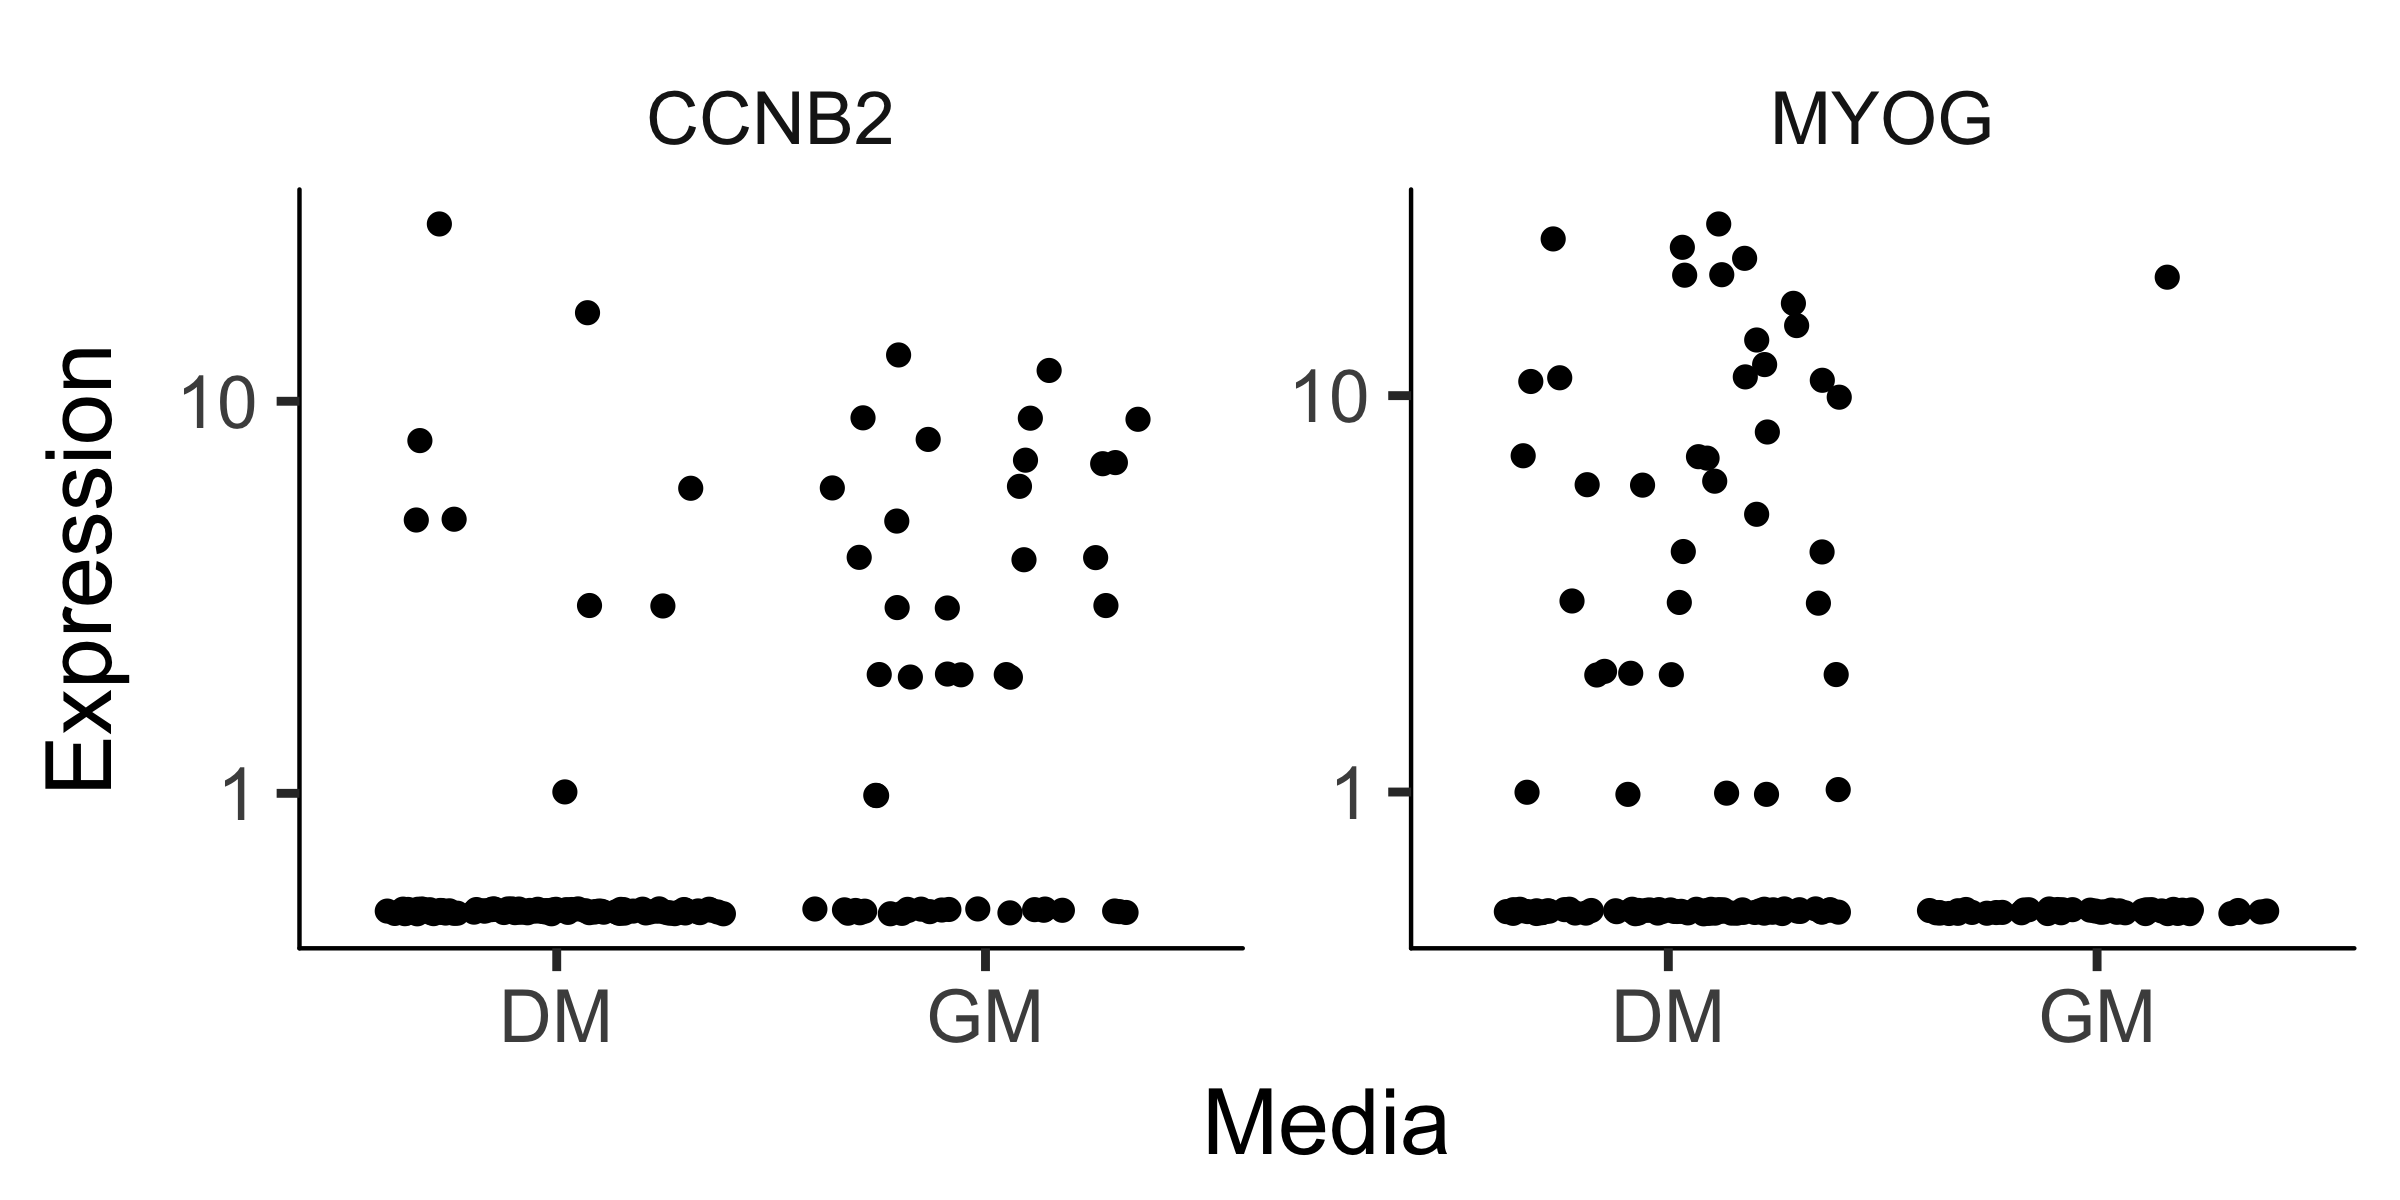
\includegraphics[width=\maxwidth]{figure/plot_myog_jitter-1} 

}



\end{knitrout}

Note that we can control how to layout the genes in the plot by specifying the number of rows and columns.  See the man page on \Rfunction{plot\_genes\_jitter} for more details on controlling its layout. Most if not all of Monocle's plotting routines return a plot object from the \Rpackage{ggplot2}.  This package uses a grammar of graphics to control various aspects of a plot, and makes it easy to customize how your data is presented.  See the \Rpackage{ggplot2} book\cite{Wickham} for more details.


In this section, we'll explore how to use Monocle to find genes that are differentially expressed according to several different criteria. First, we'll look at how to use our previous classification of the cells by type to find genes that distinguish fibroblasts and myoblasts. Second, we'll look at how to find genes that are differentially expressed as a function of pseudotime, such as those that become activated or repressed during differentiation.  Finally, you'll see how to perform multi-factorial differential analysis, which can help subtract the effects of confounding variables in your experiment.  

To keep the vignette simple and fast, we'll be working with small sets of genes. Rest assured, however, that Monocle can analyze many thousands of genes even in large experiments, making it useful for discovering dynamically regulated genes during the biological process you're studying.

\subsection{Finding genes that distinguish cell type or state}

During a dynamic biological process such as differentiation, cells might assume distinct intermediate or final states.  Recall that earlier we distinguished myoblasts from contaminating fibroblasts on the basis of several key markers. Let's look at several other genes that should distinguish between fibroblasts and myoblasts. 
\begin{knitrout}
\definecolor{shadecolor}{rgb}{0.969, 0.969, 0.969}\color{fgcolor}\begin{kframe}
\begin{alltt}
\hlstd{to_be_tested} \hlkwb{<-} \hlkwd{row.names}\hlstd{(}\hlkwd{subset}\hlstd{(}\hlkwd{fData}\hlstd{(HSMM),}
                                 \hlstd{gene_short_name} \hlopt \hlkwd{c}\hlstd{(}\hlstr{"UBC"}\hlstd{,} \hlstr{"NCAM1"}\hlstd{,} \hlstr{"ANPEP"}\hlstd{)))}
\hlstd{cds_subset} \hlkwb{<-} \hlstd{HSMM[to_be_tested,]}
\end{alltt}
\end{kframe}
\end{knitrout}

To test the effects of \Robject{CellType} on gene expression, we simply call \Rfunction{differentialGeneTest} on the genes we've selected. However, we have to specify a \emph{model formula} in the call to tell Monocle that we care about genes with expression levels that depends on \emph{CellType}.  Monocle's differential expression analysis works essentially by fitting two models to the expression values for each gene, working through each gene independently.  The first of the two models is called the \emph{full} model.  This model is essentially a way of predicting the expression value of each gene in a given cell knowing only whether that cell is a fibroblast or a myoblast.  The second model, called the \emph{reduced} model, does the same thing, but it doesn't know the \Robject{CellType} for each cell.  It has to come up with a reasonable prediction of the expression value for the gene that will be used for \emph{all} the cells. Because the full model has more information about each cell, it will do a better job of predicting the expression of the gene in each cell.  The question Monocle must answer for each gene is \emph{how much better} the full model's prediction is than the reduced model's. The greater the improvement that comes from knowing the \Robject{CellType} of each cell, the more significant the differential expression result. This is a common strategy in differential analysis, and we leave a detailed statistical exposition of such methods to others.

To set up the test based on \Robject{CellType}, we simply call \Rfunction{differentialGeneTest} with a string specifying \Robject{fullModelFormulaStr}.  We don't have to specify the reduced model in this case, because the default of \Robject{~1} is what we want here.

\begin{knitrout}
\definecolor{shadecolor}{rgb}{0.969, 0.969, 0.969}\color{fgcolor}\begin{kframe}
\begin{alltt}
\hlstd{diff_test_res} \hlkwb{<-} \hlkwd{differentialGeneTest}\hlstd{(cds_subset,}
                                      \hlkwc{fullModelFormulaStr}\hlstd{=}\hlstr{"~CellType"}\hlstd{,}
                                      \hlkwc{cores} \hlstd{=} \hlkwd{detectCores}\hlstd{())}
\hlstd{diff_test_res[,}\hlkwd{c}\hlstd{(}\hlstr{"gene_short_name"}\hlstd{,} \hlstr{"pval"}\hlstd{,} \hlstr{"qval"}\hlstd{)]}
\end{alltt}
\begin{verbatim}
##                    gene_short_name         pval         qval
## ENSG00000149294.12           NCAM1 4.505519e-92 1.351656e-91
## ENSG00000150991.10             UBC 4.000686e-01 4.000686e-01
## ENSG00000166825.9            ANPEP 4.007268e-13 6.010901e-13
\end{verbatim}
\end{kframe}
\end{knitrout}



Note that all the genes are significantly differentially expressed as a function of \Robject{CellType} except the housekeeping gene TBP, which we're using a negative control.  However, we don't know which genes correspond to myoblast-specific genes (those more highly expressed in myoblasts versus fibroblast specific genes.  We can again plot them with a jitter plot to see:

\begin{knitrout}
\definecolor{shadecolor}{rgb}{0.969, 0.969, 0.969}\color{fgcolor}\begin{kframe}
\begin{alltt}
\hlkwd{plot_genes_jitter}\hlstd{(cds_subset,} \hlkwc{grouping}\hlstd{=}\hlstr{"CellType"}\hlstd{,} \hlkwc{color_by}\hlstd{=}\hlstr{"CellType"}\hlstd{,}
                  \hlkwc{nrow}\hlstd{=}\hlnum{1}\hlstd{,} \hlkwc{ncol}\hlstd{=}\hlkwa{NULL}\hlstd{,} \hlkwc{plot_trend}\hlstd{=}\hlnum{TRUE}\hlstd{)}
\end{alltt}


{\ttfamily\noindent\itshape\color{messagecolor}{\#\# geom\_path: Each group consists of only one observation. Do you need to\\\#\# adjust the group aesthetic?\\\#\# geom\_path: Each group consists of only one observation. Do you need to\\\#\# adjust the group aesthetic?\\\#\# geom\_path: Each group consists of only one observation. Do you need to\\\#\# adjust the group aesthetic?}}\end{kframe}

{\centering 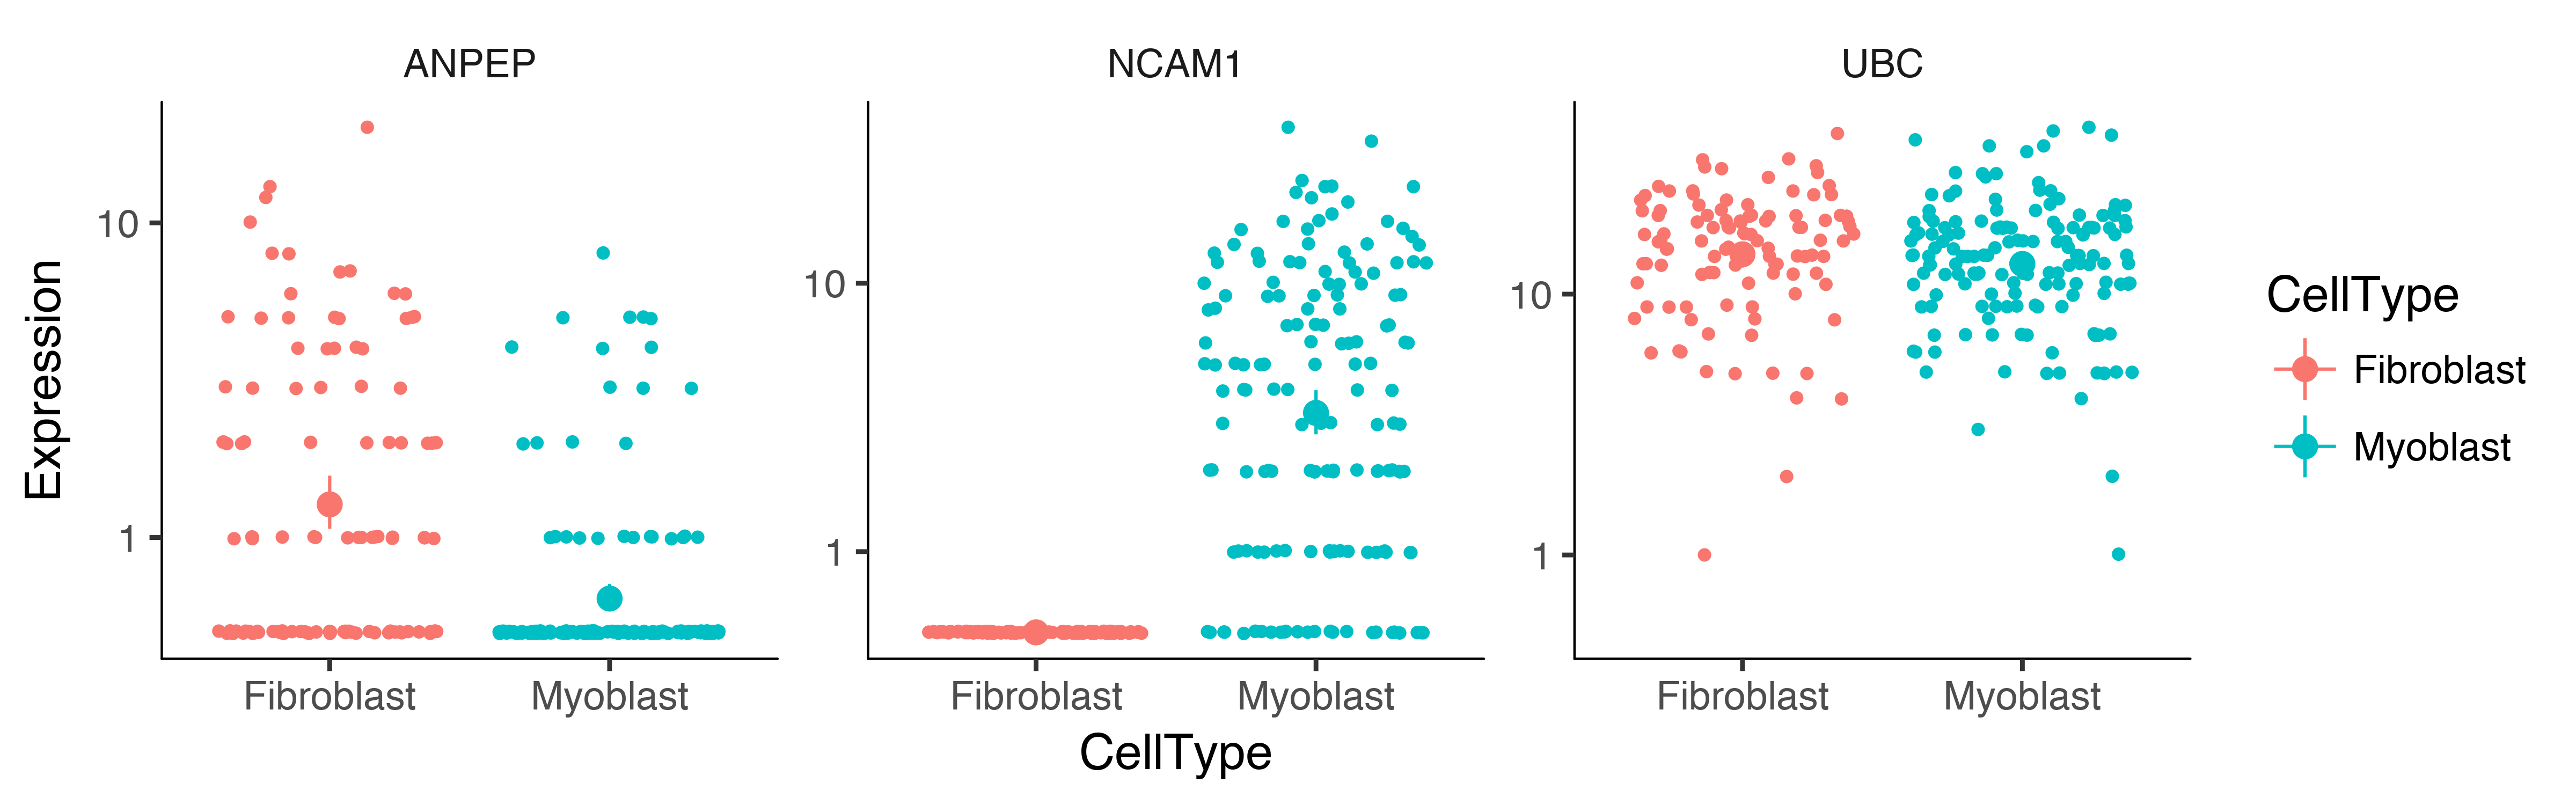
\includegraphics[width=\maxwidth]{figure/jitter_plot_diff_res-1} 

}



\end{knitrout}

Note that we could also simply compute summary statistics such as mean or median expression level on a per-\Robject{CellType} basis to see this, which might be handy if we are looking at more than a handful of genes. Of course, we could test for genes that change as a function of \Robject{Hours} to find time-varying genes, or \Robject{Media} to identify genes that are responsive to the serum switch.  In general, model formulae can contain terms in the pData table of the CellDataSet. 

The \Rfunction{differentialGeneTest} function is actually quite simple ``under the hood''.  The call above is equivalent to:
\begin{knitrout}
\definecolor{shadecolor}{rgb}{0.969, 0.969, 0.969}\color{fgcolor}\begin{kframe}
\begin{alltt}
\hlstd{full_model_fits} \hlkwb{<-} \hlkwd{fitModel}\hlstd{(cds_subset,}  \hlkwc{modelFormulaStr}\hlstd{=}\hlstr{"~CellType"}\hlstd{)}
\hlstd{reduced_model_fits} \hlkwb{<-} \hlkwd{fitModel}\hlstd{(cds_subset,} \hlkwc{modelFormulaStr}\hlstd{=}\hlstr{"~1"}\hlstd{)}
\hlstd{diff_test_res} \hlkwb{<-} \hlkwd{compareModels}\hlstd{(full_model_fits, reduced_model_fits)}
\hlstd{diff_test_res}
\end{alltt}
\end{kframe}
\end{knitrout}
Occassionally, as we'll see later, it's useful to be able to call \Rfunction{fitModel} directly.

The differential analysis procedure in Monocle is extremely flexible: the model formulae you use in your tests can include any term that exists as a column in the \Rfunction{pData} table, including those columns that are added by Monocle in other analysis steps. For example, if you use \Rfunction{clusterCells()}, you can test for genes that differ between clusters by using \Robject{Cluster} as your model formula.

\subsection{Finding genes that change as a function of pseudotime} \label{pseudotime_diff}

Monocle's main job is to put cells in order of progress through a biological process (such as cell differentiation) without knowing which genes to look at ahead of time.  Once it's done so, you can analyze the cells to find genes that changes as the cells make progress.  For example, you can find genes that are significantly upregulated as the cells ``mature''.  Let's look at a panel of genes important for myogenesis: 

\begin{knitrout}
\definecolor{shadecolor}{rgb}{0.969, 0.969, 0.969}\color{fgcolor}\begin{kframe}
\begin{alltt}
\hlstd{to_be_tested} \hlkwb{<-} \hlkwd{row.names}\hlstd{(}\hlkwd{subset}\hlstd{(}\hlkwd{fData}\hlstd{(HSMM),}
                                 \hlstd{gene_short_name} \hlopt \hlkwd{c}\hlstd{(}\hlstr{"MYH3"}\hlstd{,} \hlstr{"MEF2C"}\hlstd{,} \hlstr{"CCNB2"}\hlstd{,} \hlstr{"TNNT1"}\hlstd{)))}
\hlstd{cds_subset} \hlkwb{<-} \hlstd{HSMM_myo[to_be_tested,]}
\end{alltt}
\end{kframe}
\end{knitrout}

Again, we'll need to specify the model we want to use for differential analysis.  This model will be a bit more complicated than the one we used to look at the differences between \Robject{CellType}.  Monocle assigns each cell a ``pseudotime'' value, which records its progress through the process in the experiment.  The model can test against changes as a function of this value. Monocle uses the \Rpackage{VGAM} package to model a gene's expression level as a smooth, nonlinear function of pseudotime:
\begin{knitrout}
\definecolor{shadecolor}{rgb}{0.969, 0.969, 0.969}\color{fgcolor}\begin{kframe}
\begin{alltt}
\hlstd{diff_test_res} \hlkwb{<-} \hlkwd{differentialGeneTest}\hlstd{(cds_subset,}
                                      \hlkwc{fullModelFormulaStr}\hlstd{=}\hlstr{"~sm.ns(Pseudotime)"}\hlstd{,}
                                      \hlkwc{cores} \hlstd{=} \hlkwd{detectCores}\hlstd{())}
\end{alltt}
\end{kframe}
\end{knitrout}



The \Rfunction{sm.ns} function states that Monocle should fit a natural spline through the expression values to help it describe the changes in expression as a function of progress. We'll see what this trend looks like in just a moment. Other smoothing functions are available.

Once again, let's add in the gene annotations so it's easy to see which genes are significant.
\begin{knitrout}
\definecolor{shadecolor}{rgb}{0.969, 0.969, 0.969}\color{fgcolor}\begin{kframe}
\begin{alltt}
\hlstd{diff_test_res[,}\hlkwd{c}\hlstd{(}\hlstr{"gene_short_name"}\hlstd{,} \hlstr{"pval"}\hlstd{,} \hlstr{"qval"}\hlstd{)]}
\end{alltt}
\begin{verbatim}
##                    gene_short_name         pval         qval
## ENSG00000081189.9            MEF2C 6.134750e-35 1.226950e-34
## ENSG00000105048.12           TNNT1 3.141574e-33 3.141574e-33
## ENSG00000109063.9             MYH3 6.124129e-71 2.449651e-70
## ENSG00000157456.3            CCNB2 3.907668e-34 5.210224e-34
\end{verbatim}
\end{kframe}
\end{knitrout}

We can plot the expression levels of these genes, all of which show significant changes as a function of differentiation, using the function \Rfunction{plot\_genes\_in\_pseudotime}. This function has a number of cosmetic options you can use to control the layout and appearance of your plot.

\begin{knitrout}
\definecolor{shadecolor}{rgb}{0.969, 0.969, 0.969}\color{fgcolor}\begin{kframe}
\begin{alltt}
\hlkwd{plot_genes_in_pseudotime}\hlstd{(cds_subset,} \hlkwc{color_by}\hlstd{=}\hlstr{"Hours"}\hlstd{)}
\end{alltt}
\end{kframe}

{\centering 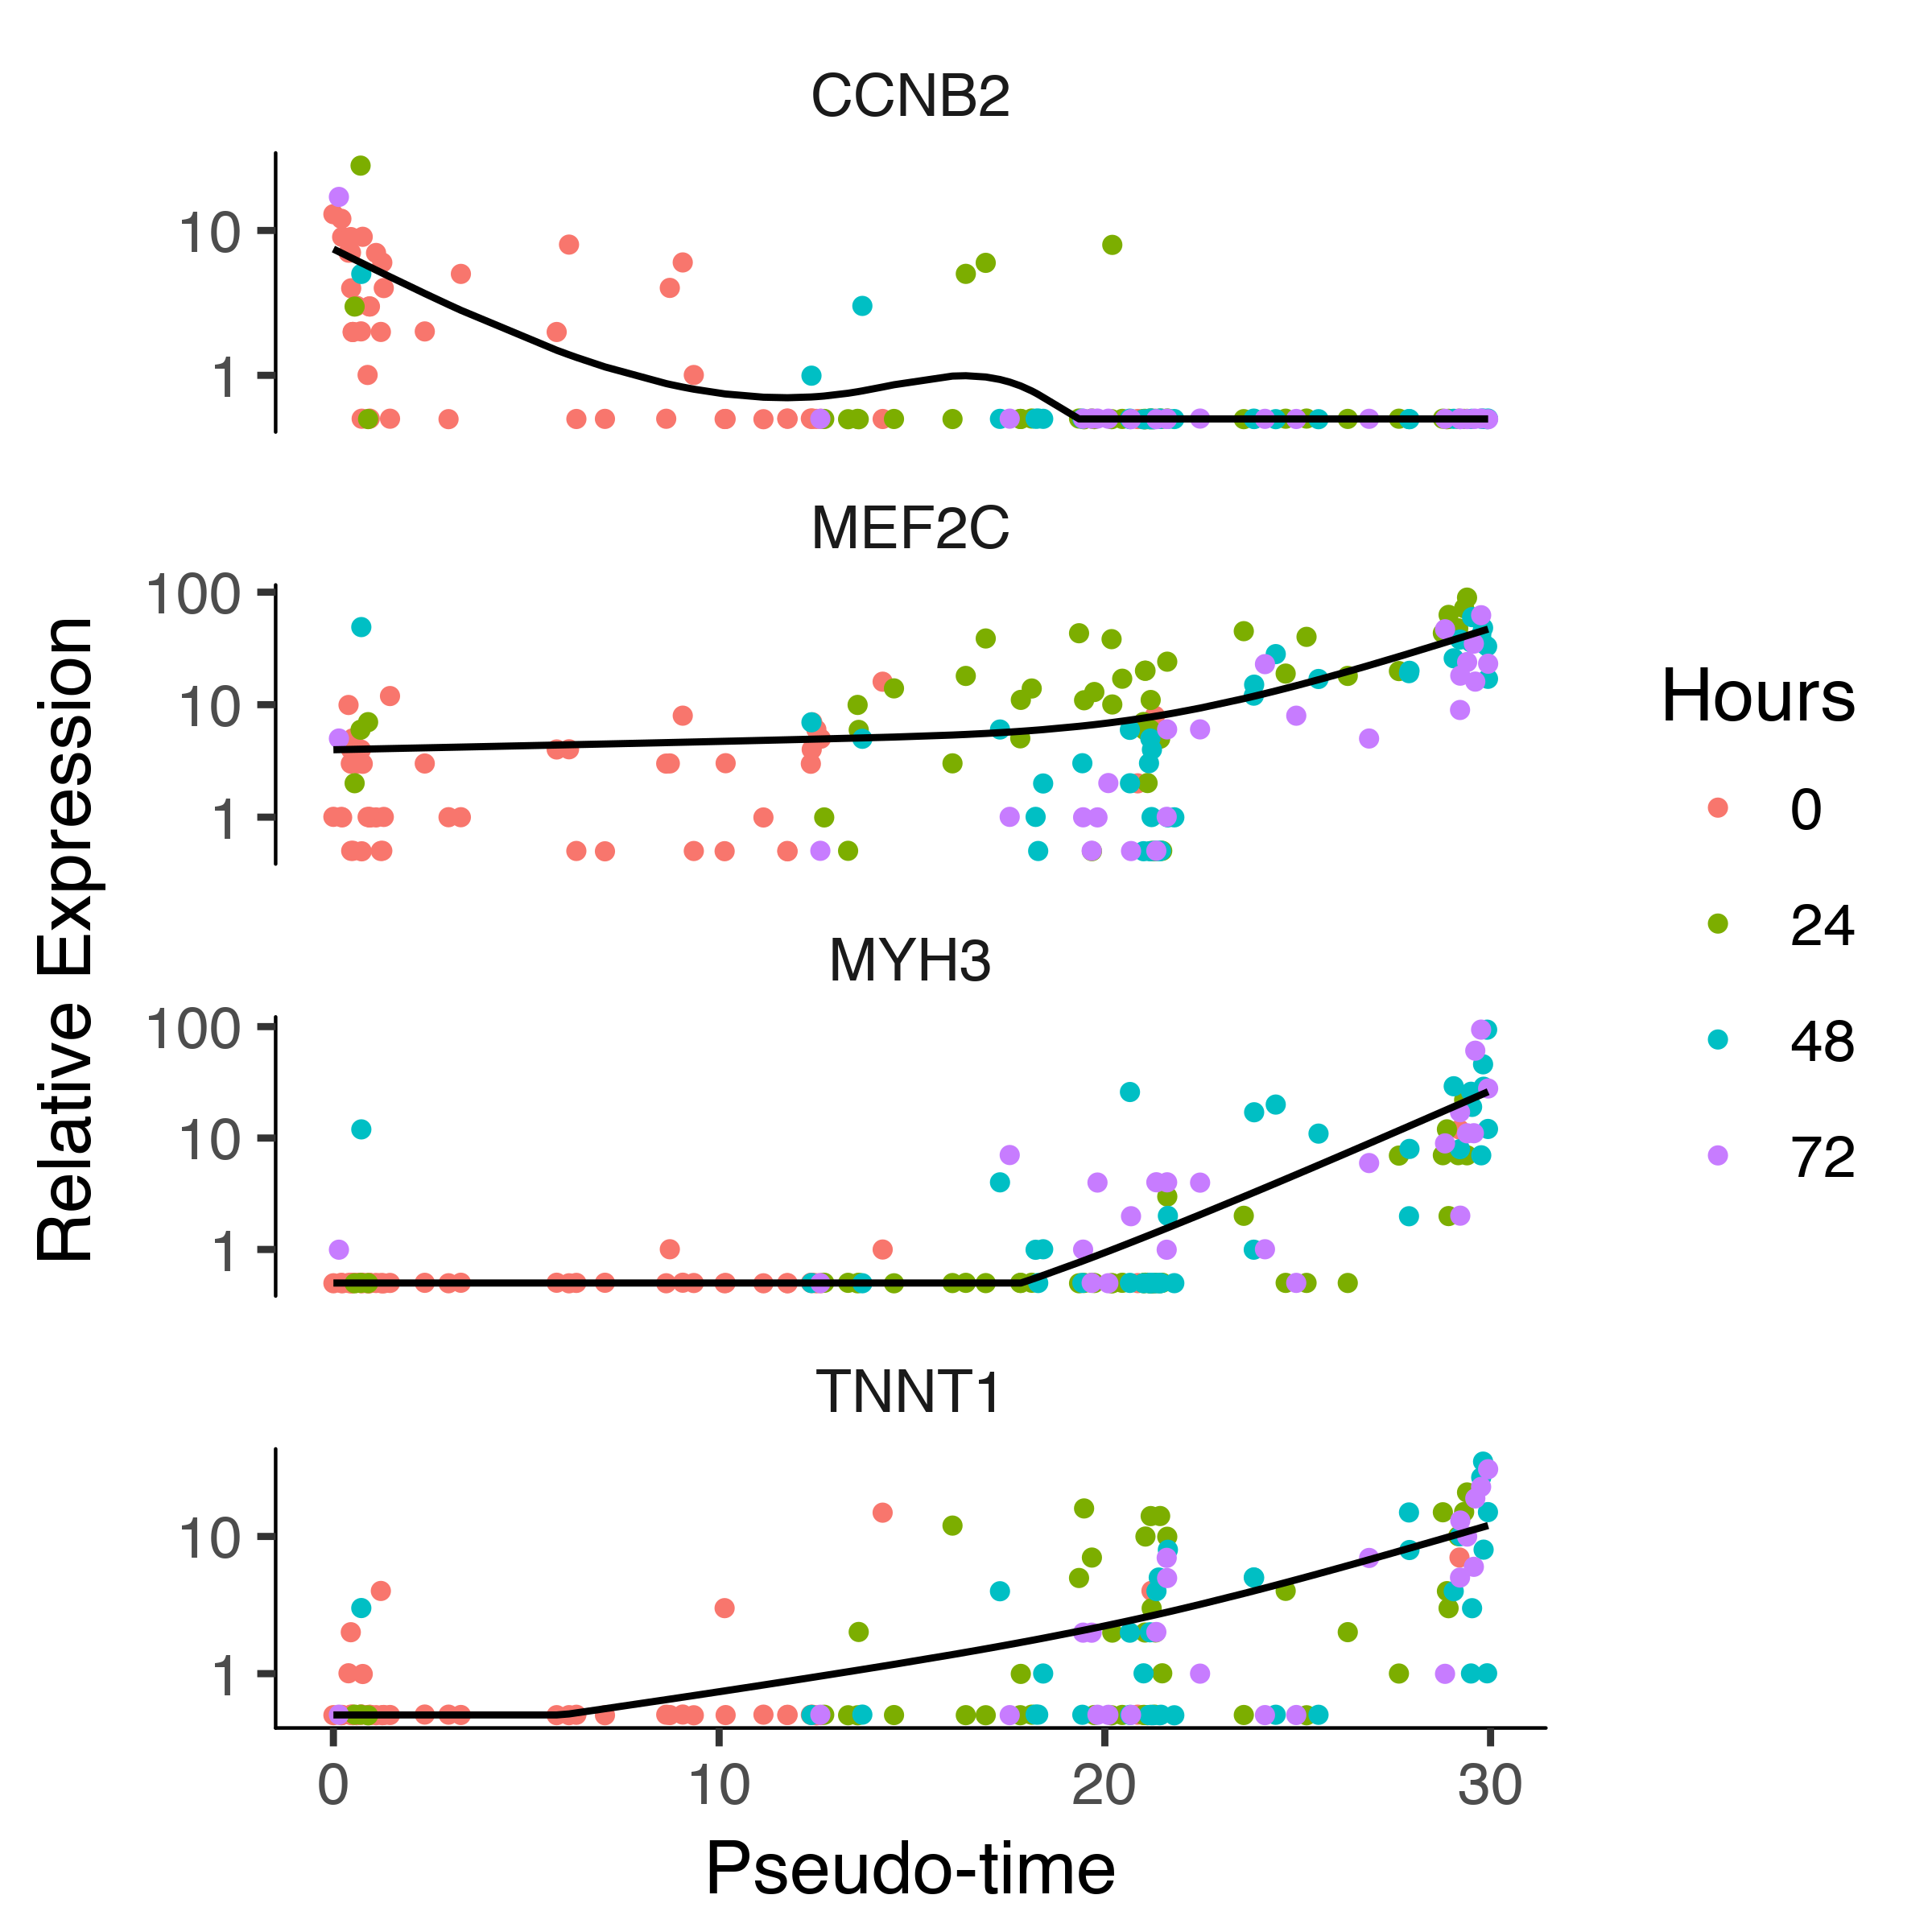
\includegraphics[width=\maxwidth]{figure/plot_diff_res_pt-1} 

}



\end{knitrout}

\subsection{Clustering genes by pseudotemporal expression pattern}

A common question that arises when studying time-series gene expression studies is: ``which genes follow similar kinetic trends''?  Monocle can help you answer this question by grouping genes that have similar trends, so you can analyze these groups to see what they have in common.  Monocle provides a convenient way to visualize all pseudotime-dependent genes. The function
\Rfunction{plot\_pseudotime\_heatmap} takes a CellDataSet object (usually containing a only subset of significant genes)
and generates smooth expression curves much like  \Rfunction{plot\_genes\_in\_pseudotime}. Then, it clusters these genes 
and plots them using the \Rpackage{pheatmap} package.  This allows you to visualize modules of genes that
co-vary across pseudotime.

\begin{knitrout}
\definecolor{shadecolor}{rgb}{0.969, 0.969, 0.969}\color{fgcolor}\begin{kframe}
\begin{alltt}
\hlstd{diff_test_res} \hlkwb{<-} \hlkwd{differentialGeneTest}\hlstd{(HSMM_myo[marker_genes,],}
                                      \hlkwc{fullModelFormulaStr}\hlstd{=}\hlstr{"~sm.ns(Pseudotime)"}\hlstd{,}
                                      \hlkwc{cores} \hlstd{=} \hlkwd{detectCores}\hlstd{())}

\hlstd{sig_gene_names} \hlkwb{<-} \hlkwd{row.names}\hlstd{(}\hlkwd{subset}\hlstd{(diff_test_res, qval} \hlopt{<} \hlnum{0.1}\hlstd{))}


\hlkwd{plot_pseudotime_heatmap}\hlstd{(HSMM_myo[sig_gene_names,],}
                        \hlkwc{num_clusters} \hlstd{=} \hlnum{3}\hlstd{,}
                        \hlkwc{cores} \hlstd{=} \hlkwd{detectCores}\hlstd{(),}
                        \hlkwc{show_rownames} \hlstd{= T)}
\end{alltt}
\end{kframe}

{\centering 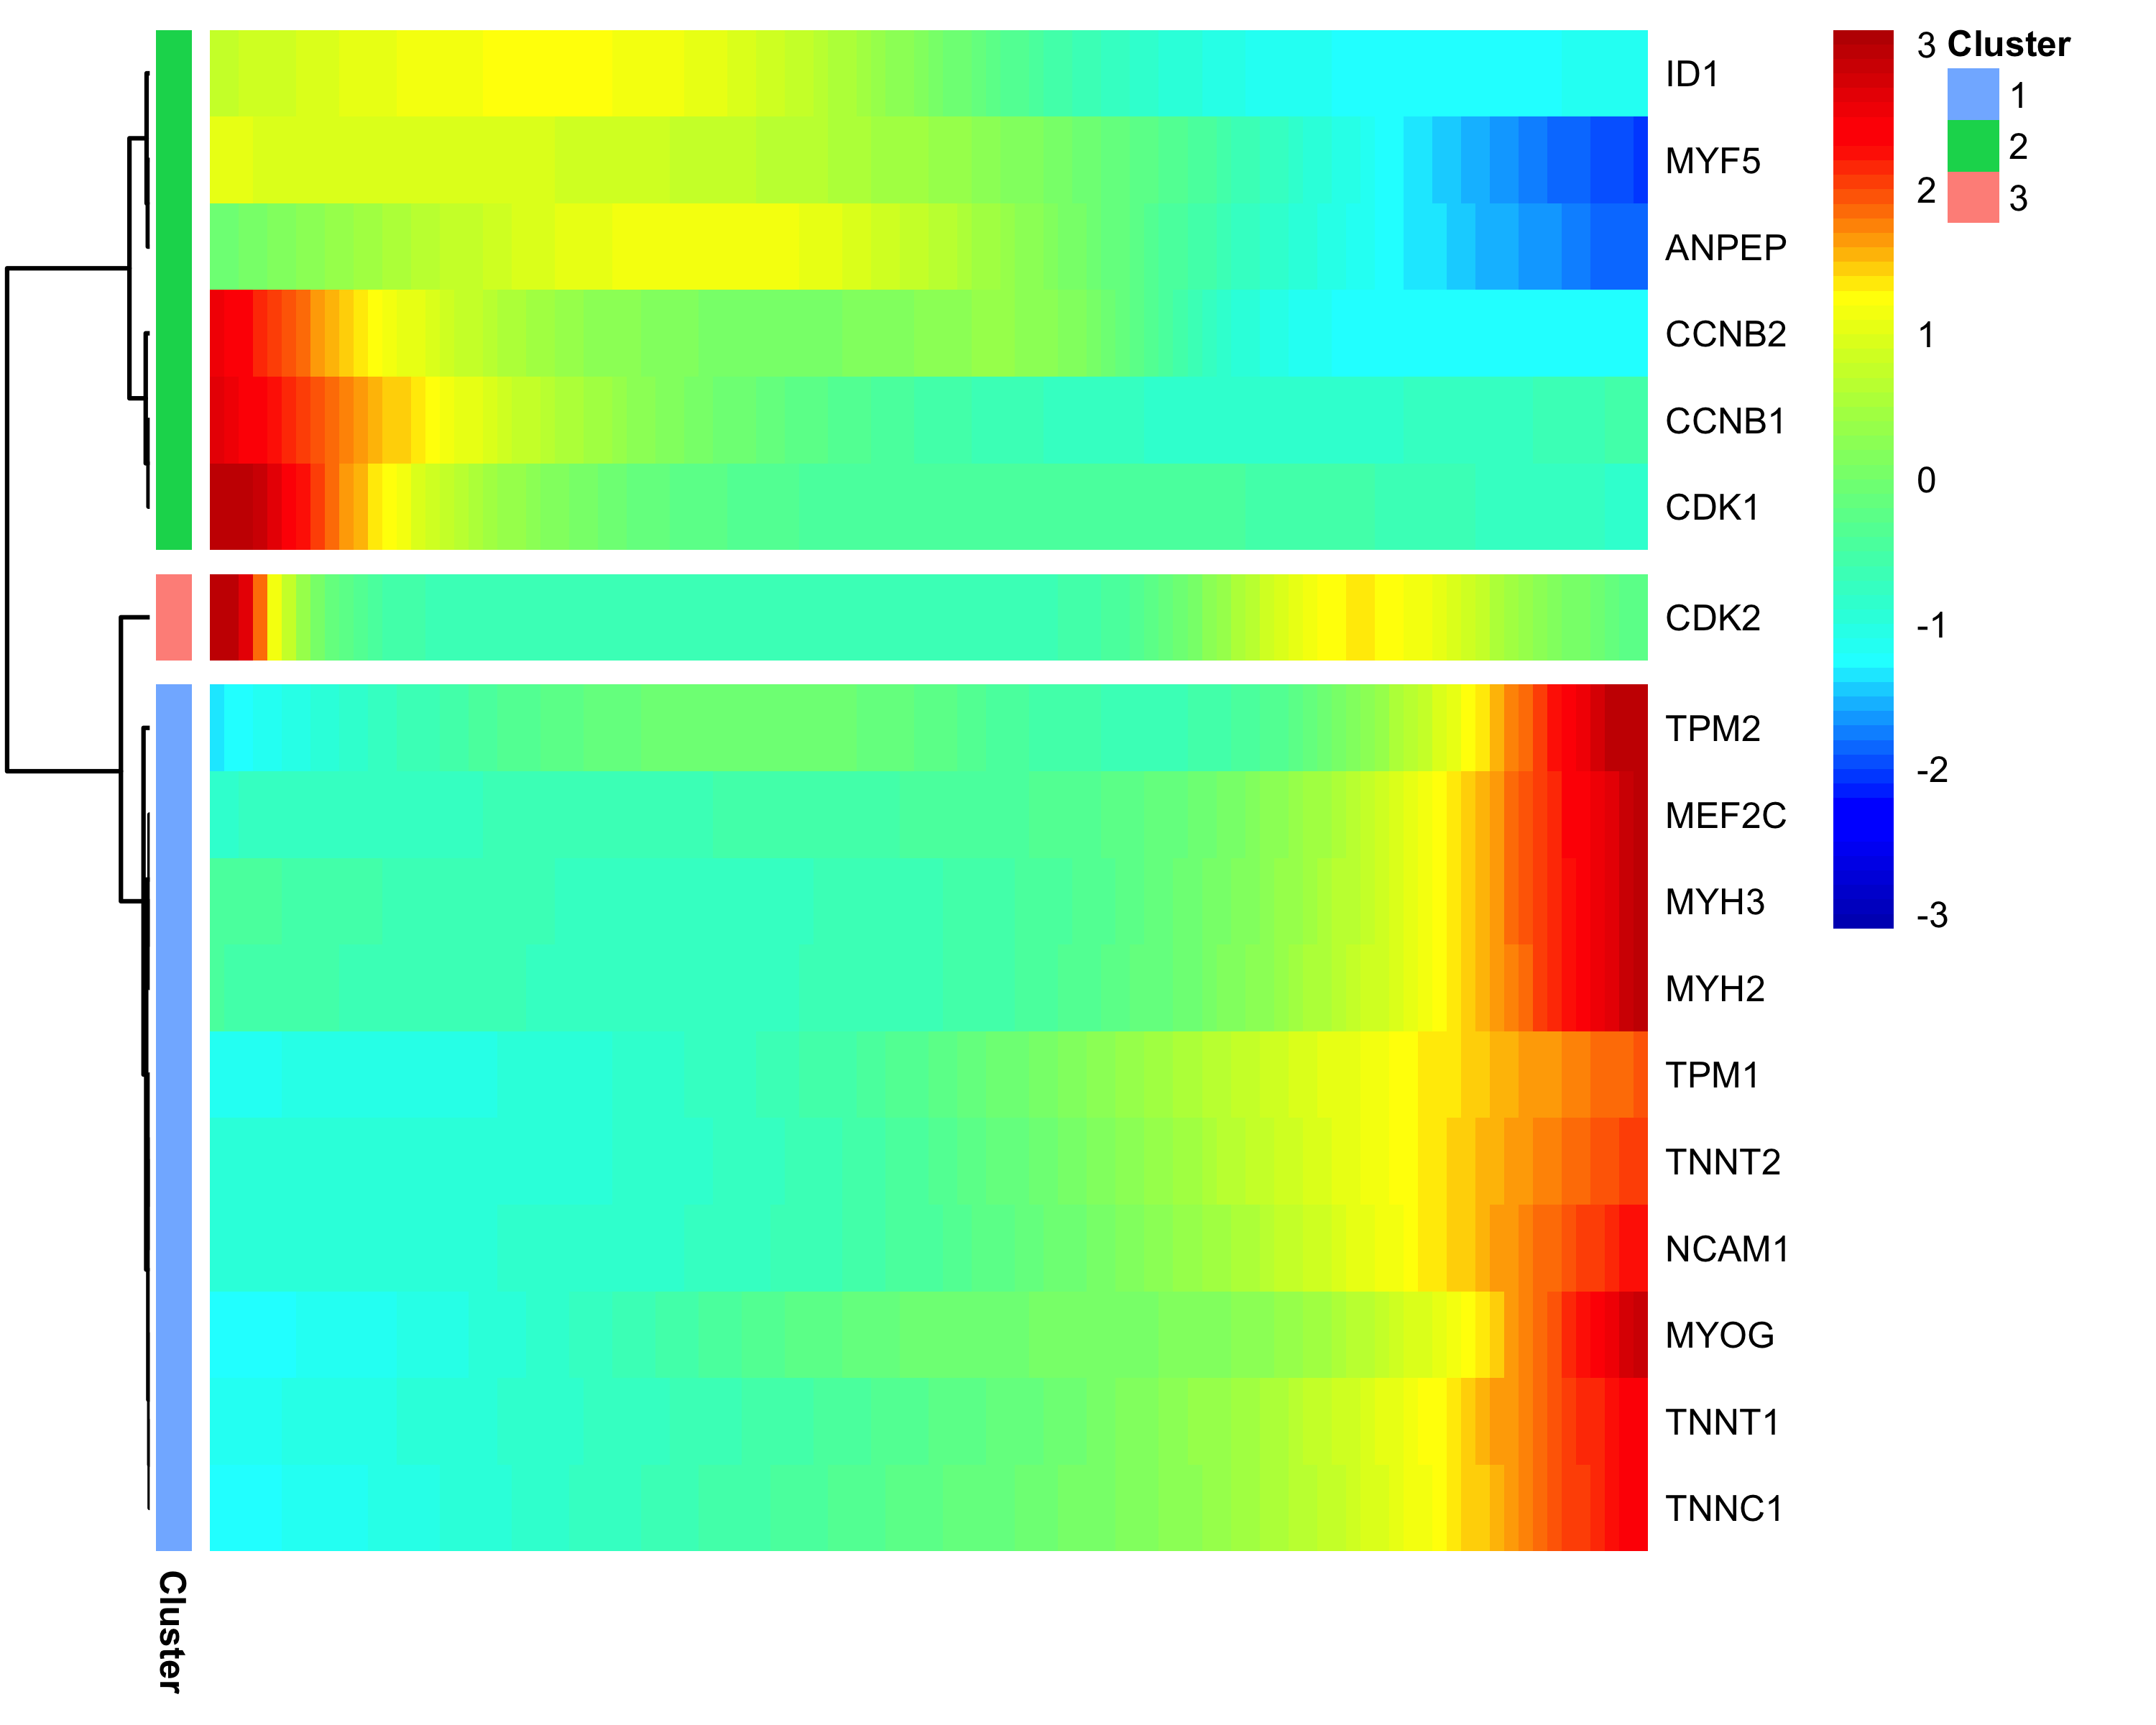
\includegraphics[width=\maxwidth]{figure/plot_diff_res_pt_heatmap-1} 

}



\end{knitrout}



\subsection{Multi-factorial differential expression analysis}

Monocle can perform differential analysis in the presence of multiple factors, which can help you subtract some factors to see the effects of others.  In the simple example below, Monocle tests three genes for differential expression between myoblasts and fibroblasts, while subtracting the effect of \Robject{Hours}, which encodes the day on which each cell was collected. To do this, we must specify both the full model and the reduced model. The full model captures the effects of both \Robject{CellType} and \Robject{Hours}, while the reduced model only knows about \Robject{Hours}.  

When we plot the expression levels of these genes, we can modify the resulting object returned by \Rfunction{plot\_genes\_jitter} to allow them to have independent y-axis ranges, to better highlight the differences between cell states.

\begin{knitrout}
\definecolor{shadecolor}{rgb}{0.969, 0.969, 0.969}\color{fgcolor}\begin{kframe}
\begin{alltt}
\hlstd{to_be_tested} \hlkwb{<-} \hlkwd{row.names}\hlstd{(}\hlkwd{subset}\hlstd{(}\hlkwd{fData}\hlstd{(HSMM),}
                                 \hlstd{gene_short_name} \hlopt \hlkwd{c}\hlstd{(}\hlstr{"TPM1"}\hlstd{,} \hlstr{"MYH3"}\hlstd{,} \hlstr{"CCNB2"}\hlstd{,} \hlstr{"GAPDH"}\hlstd{)))}
\hlstd{cds_subset} \hlkwb{<-} \hlstd{HSMM[to_be_tested,]}

\hlstd{diff_test_res} \hlkwb{<-} \hlkwd{differentialGeneTest}\hlstd{(cds_subset,}
                                      \hlkwc{fullModelFormulaStr}\hlstd{=}\hlstr{"~CellType + Hours"}\hlstd{,}
                                      \hlkwc{reducedModelFormulaStr}\hlstd{=}\hlstr{"~Hours"}\hlstd{,}
                                      \hlkwc{cores} \hlstd{=} \hlkwd{detectCores}\hlstd{())}
\hlstd{diff_test_res[,}\hlkwd{c}\hlstd{(}\hlstr{"gene_short_name"}\hlstd{,} \hlstr{"pval"}\hlstd{,} \hlstr{"qval"}\hlstd{)]}
\end{alltt}
\begin{verbatim}
##                    gene_short_name         pval         qval
## ENSG00000109063.9             MYH3 4.990678e-55 1.996271e-54
## ENSG00000111640.10           GAPDH 1.974650e-01 1.974650e-01
## ENSG00000140416.15            TPM1 2.540899e-22 5.081798e-22
## ENSG00000157456.3            CCNB2 1.358945e-02 1.811926e-02
\end{verbatim}
\begin{alltt}
\hlkwd{plot_genes_jitter}\hlstd{(cds_subset,}
                  \hlkwc{grouping}\hlstd{=}\hlstr{"Hours"}\hlstd{,} \hlkwc{color_by}\hlstd{=}\hlstr{"CellType"}\hlstd{,} \hlkwc{plot_trend}\hlstd{=}\hlnum{TRUE}\hlstd{)} \hlopt{+}
  \hlkwd{facet_wrap}\hlstd{(} \hlopt{~} \hlstd{feature_label,} \hlkwc{scales}\hlstd{=}\hlstr{"free_y"}\hlstd{)}
\end{alltt}
\end{kframe}

{\centering 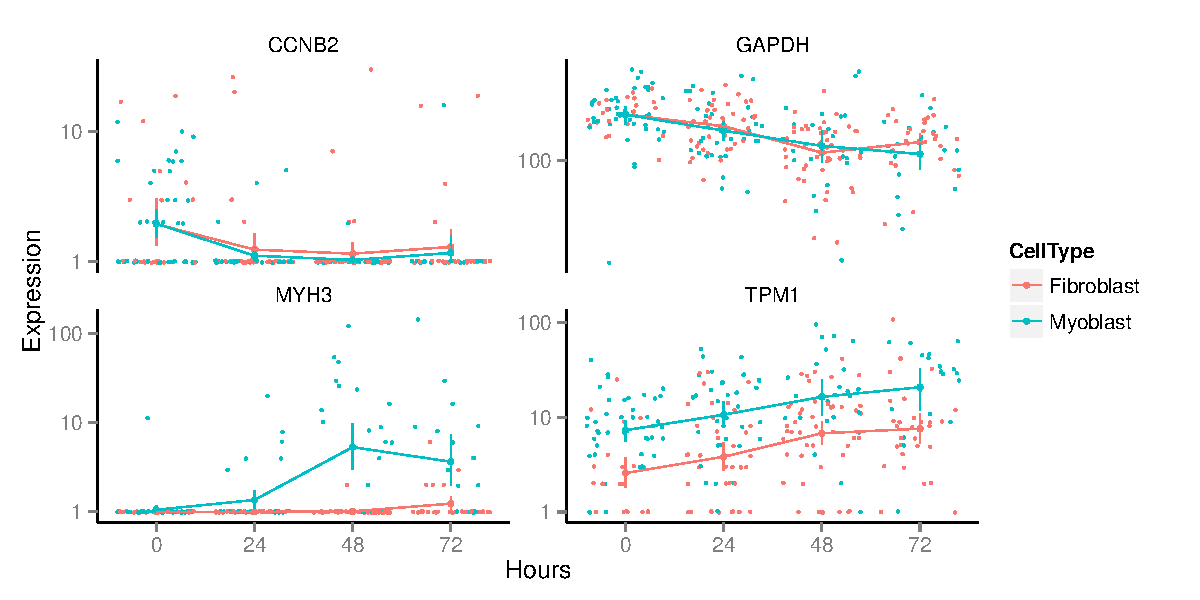
\includegraphics[width=\maxwidth]{figure/plot_diff_res_multi-1} 

}



\end{knitrout}



\section{Analyzing branches in single-cell trajectories} \label{BEAM_trajectory}

Often, single-cell trajectories include branches. The branches occur because cells execute alternative gene expression programs. Branches appear in trajectories during development, when cells make fate choices: one developmental lineage proceeds down one path, while the other lineage produces a second path. Monocle contains extensive functionality for analyzing these branching events. 

Consider the experiment performed by Steve Quake's lab by Barbara Treutlein and colleages, who captured cells from the developing mouse lung. They captured cells early in development, later when the lung contains both major types of epithelial cells (AT1 and AT2), and cells right about to make the decision to become either AT1 or AT2. Monocle can reconstruct this process as a \emph{branched} trajectory, allow you to analyze the decision point in great detail. We'll learn more about branch analysis in section \ref{BEAM}. The figure below shows the trajectory Monocle reconstructs using some of their data. There is a single branch, labeled "1". What genes change as cells pass from the early developmental stage the top left of the tree through the branch? What genes are differentially expressed between the branches? To answer this question, Monocle provides you with a special statistical test: branched expression analysis modeling, or BEAM.

\begin{knitrout}
\definecolor{shadecolor}{rgb}{0.969, 0.969, 0.969}\color{fgcolor}\begin{kframe}
\begin{alltt}
\hlstd{lung} \hlkwb{<-} \hlkwd{load_lung}\hlstd{()}
\end{alltt}


{\ttfamily\noindent\itshape\color{messagecolor}{\#\# Removing 4 outliers}}\begin{alltt}
\hlkwd{plot_cell_trajectory}\hlstd{(lung,} \hlkwc{color_by}\hlstd{=}\hlstr{"Time"}\hlstd{)}
\end{alltt}
\end{kframe}

{\centering 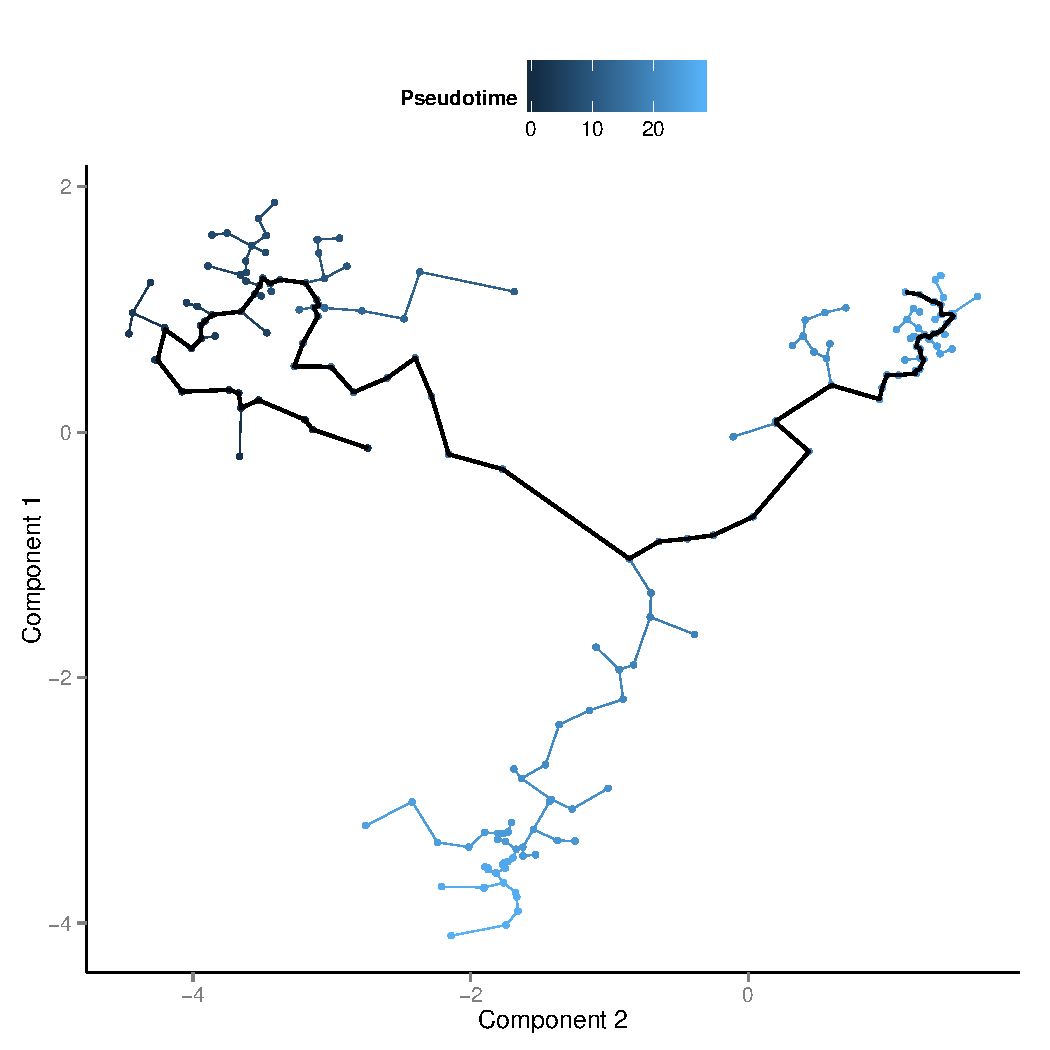
\includegraphics[width=\maxwidth]{figure/init_treutlein-1} 

}



\end{knitrout}

BEAM takes as input a CellDataSet that's been ordered with \Rfunction{orderCells} and the name of a branch point in the trajectory. It returns a table of significance scores for each gene. Genes that score significant are said to be \emph{branch-dependent} in their expression.

\begin{knitrout}
\definecolor{shadecolor}{rgb}{0.969, 0.969, 0.969}\color{fgcolor}\begin{kframe}
\begin{alltt}
\hlstd{BEAM_res} \hlkwb{<-} \hlkwd{BEAM}\hlstd{(lung,} \hlkwc{branch_point}\hlstd{=}\hlnum{1}\hlstd{,} \hlkwc{cores} \hlstd{=} \hlkwd{detectCores}\hlstd{())}
\hlstd{BEAM_res} \hlkwb{<-} \hlstd{BEAM_res[}\hlkwd{order}\hlstd{(BEAM_res}\hlopt{$}\hlstd{qval),]}
\hlstd{BEAM_res} \hlkwb{<-} \hlstd{BEAM_res[,}\hlkwd{c}\hlstd{(}\hlstr{"gene_short_name"}\hlstd{,} \hlstr{"pval"}\hlstd{,} \hlstr{"qval"}\hlstd{)]}
\end{alltt}
\end{kframe}
\end{knitrout}



You can visualize changes for all the genes that are significantly branch dependent using a special type of heatmap. This heatmap shows changes in both lineages at the same time. It also requires that you choose a branch point to inspect. Columns are points in pseudotime, rows are genes, and the beginning of pseudotime is in the middle of the heatmap. As you read from the middle of the heatmap to the right, you are following one lineage through pseudotime. As you read left, the other. The genes are clustered hierarchically, so you can visualize modules of genes that have similar lineage-dependent expression patterns.
\begin{knitrout}
\definecolor{shadecolor}{rgb}{0.969, 0.969, 0.969}\color{fgcolor}\begin{kframe}
\begin{alltt}
\hlkwd{plot_genes_branched_heatmap}\hlstd{(lung[}\hlkwd{row.names}\hlstd{(}\hlkwd{subset}\hlstd{(BEAM_res, qval} \hlopt{<} \hlnum{1e-4}\hlstd{)),],}
                            \hlkwc{branch_point} \hlstd{=} \hlnum{1}\hlstd{,}
                            \hlkwc{num_clusters} \hlstd{=} \hlnum{4}\hlstd{,}
                            \hlkwc{cores} \hlstd{=} \hlkwd{detectCores}\hlstd{(),}
                            \hlkwc{use_gene_short_name} \hlstd{= T,}
                            \hlkwc{show_rownames} \hlstd{= T)}
\end{alltt}
\end{kframe}

{\centering 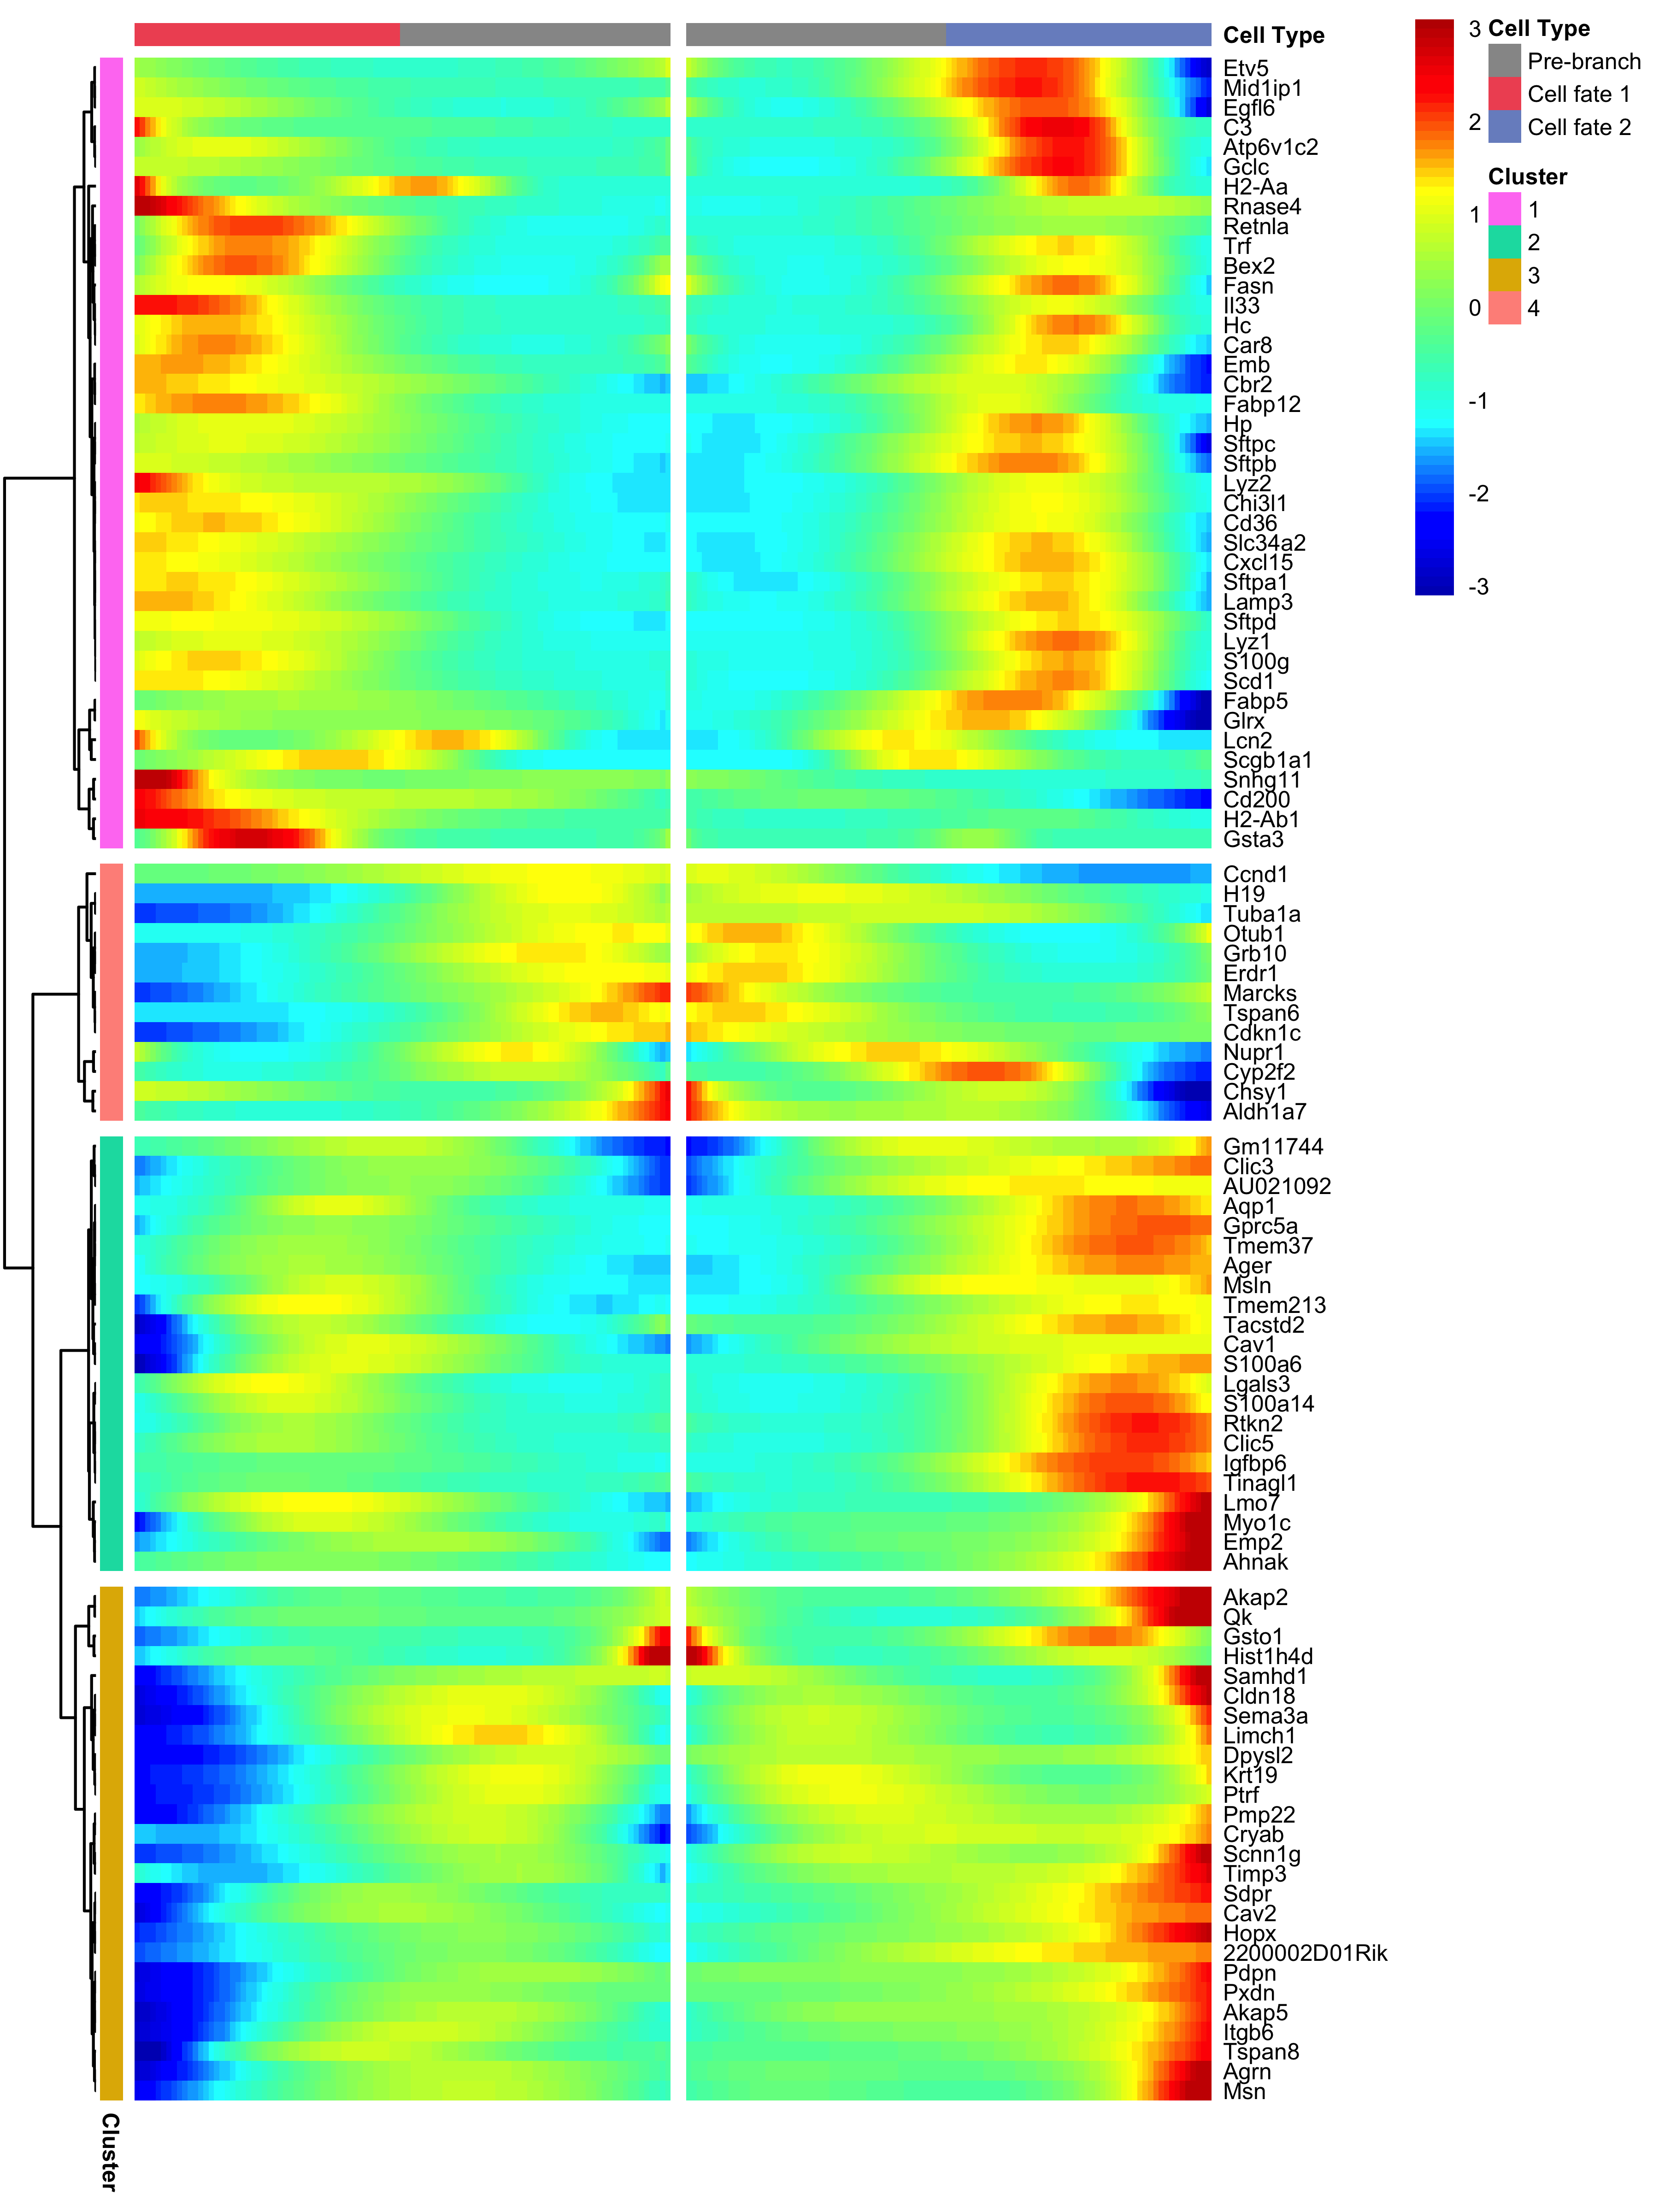
\includegraphics[width=\maxwidth]{figure/lung_beam_branched_heatmap-1} 

}



\end{knitrout}



We can plot a couple of these genes, such as \emph{Pdpn} and \emph{Sftpb} (both known markers of fate in this system), using the \Rfunction{plot\_genes\_branched\_pseudotime} function, which works a lot like the \Rfunction{plot\_genes\_in\_pseudotime} function, except it shows two kinetic trends, one for each lineage, instead of one. We also show \emph{Ccnd2}, a cell cycle gene, which is downregulated in both branches and is not signficant by the BEAM test. 

\begin{knitrout}
\definecolor{shadecolor}{rgb}{0.969, 0.969, 0.969}\color{fgcolor}\begin{kframe}
\begin{alltt}
\hlstd{lung_genes} \hlkwb{<-} \hlkwd{row.names}\hlstd{(}\hlkwd{subset}\hlstd{(}\hlkwd{fData}\hlstd{(lung), gene_short_name} \hlopt \hlkwd{c}\hlstd{(}\hlstr{"Ccnd2"}\hlstd{,} \hlstr{"Sftpb"}\hlstd{,} \hlstr{"Pdpn"}\hlstd{)))}
\hlkwd{plot_genes_branched_pseudotime}\hlstd{(lung[lung_genes,],}
                               \hlkwc{branch_point}\hlstd{=}\hlnum{1}\hlstd{,}
                               \hlkwc{color_by}\hlstd{=}\hlstr{"Time"}\hlstd{,}
                               \hlkwc{ncol}\hlstd{=}\hlnum{1}\hlstd{)}
\end{alltt}
\end{kframe}

{\centering 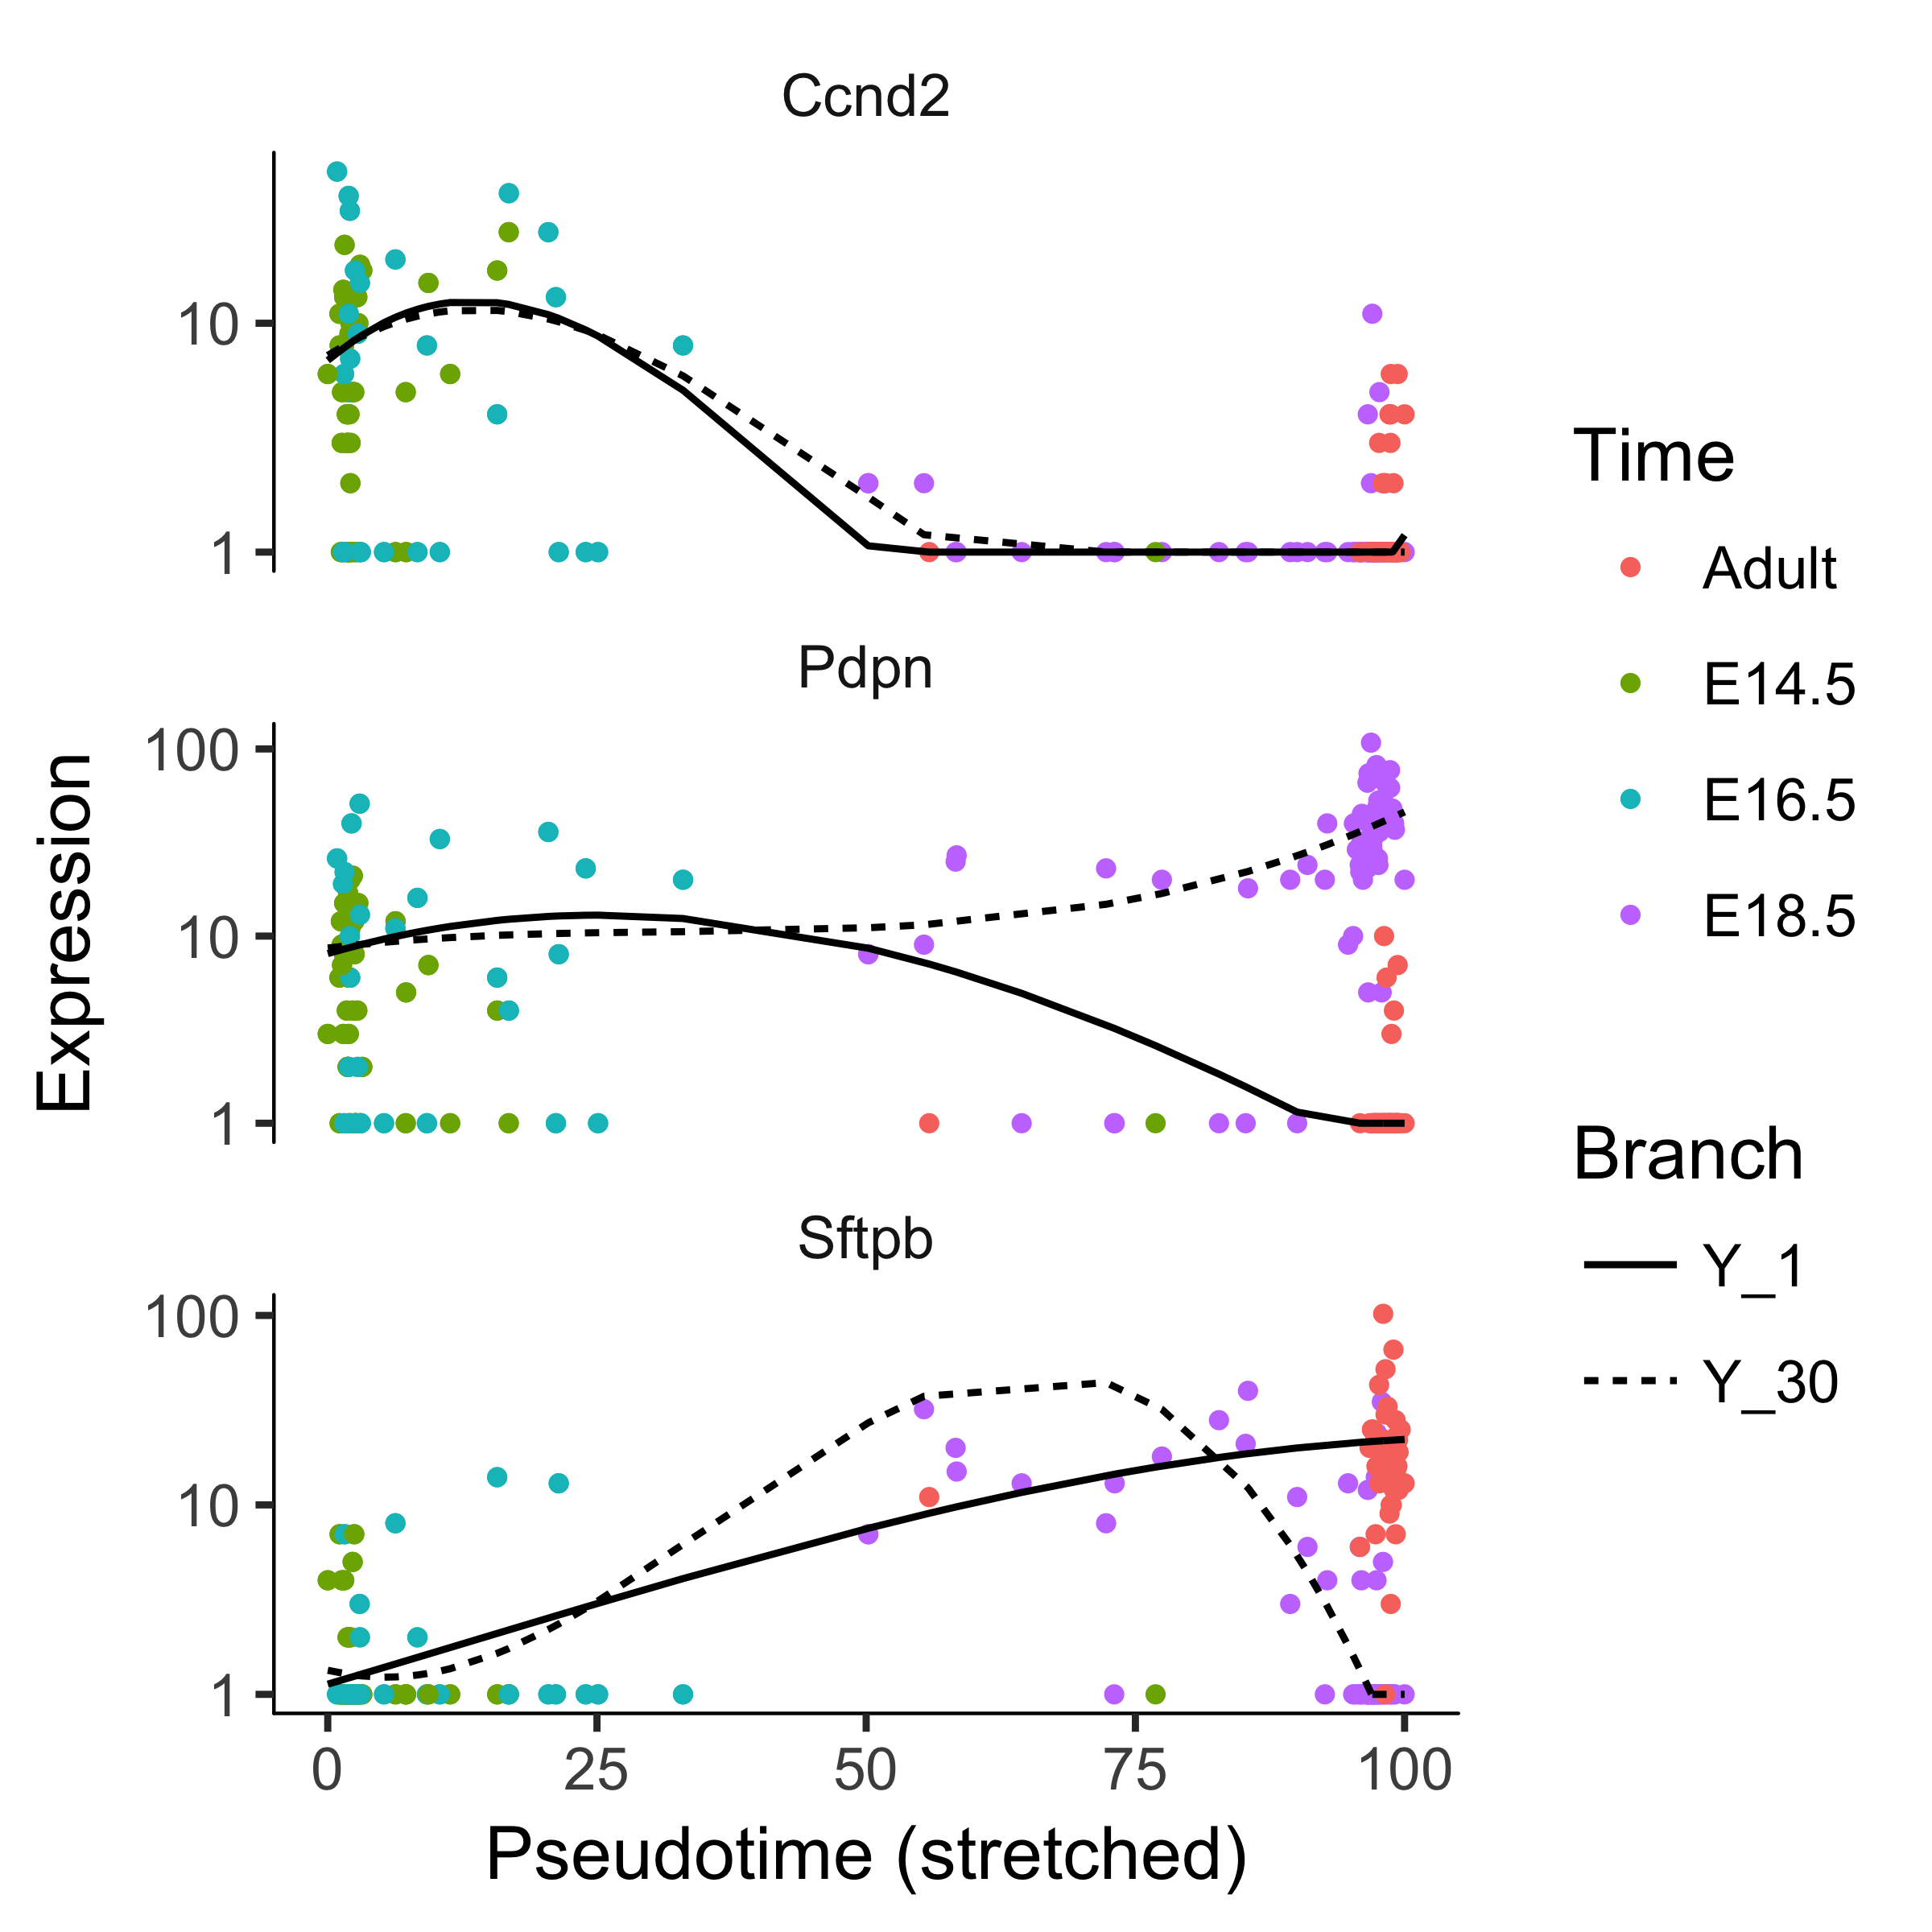
\includegraphics[width=\maxwidth]{figure/lung_beam_branched_pseudotime-1} 

}



\end{knitrout}

The \Rfunction{plot\_clusters} function returns a ggplot2 object showing the shapes of the expression patterns followed by the 100 genes we've picked out.  The topographic lines highlight the distributions of the kinetic patterns relative to the overall trend lines, shown in red.




 %\section{Tips and tricks}

\section{Major changes between Monocle version 1 and version 2}
Monocle 2 is a near-complete re-write of Monocle 1. Monocle 2 is geared towards larger, more complex single-cell RNA-Seq experiments than those possible at the time Monocle 1 was written. It's also redesigned to support analysis of mRNA counts, which were hard to estimate experimentally in early versions of single-cell RNA-Seq. Now, with spike controls or UMIs, gene expression can  be measured in mRNA counts. Analysis of these counts is typically easier and more accurate than relative expression values, and we encourage all users to adopt an mRNA-count centered workflow. Numerous Monocle functions have been re-written to take advantage of the nicer statistical properties of mRNA counts. For example, we adopt the dispersion modeling and variance-stabilization techniques introduced by DESeq \cite{Anders2010-oc} during differential analysis, dimensionality reduction, and other steps. 
 
Trajectory reconstruction in Monocle 2 is vastly more robust, faster, and more powerful than in Monocle 1. Monocle 2 uses an advanced nonlinear reconstruction algorithm called DDRTree\cite{Mao2015-cs}, described below in section \ref{theory}. This algorithm can expose branches that are hard to see with the less powerful linear technique used in Monocle 1. The algorithm is also far less sensitive to outliers, so careful QC and selection of high quality cells is less critical.  Finally, DDRTree is much more robust in that it reports qualititatively similar trajectories more consistently when you vary the number of cells in the experiment. Although which genes are included in the ordering still greatly impact the trajectory, varying them also produces more qualititatively consistent trajectories than the previous linear technique.
 
Because Monocle 2 is so much better at finding branches, it also includes some additional tools to help you interpret them. Branch expression analysis modeling (BEAM) is a new test for analyzing specific branch points\cite{qiu2017single}. BEAM reports branch-dependent genes, and Monocle 2 includes some new visualization functions to help you inspect these genes. Overall, we find that branching is pervasive in diverse biological processes, and thus we expect BEAM will be very useful to those analyzing single-cell RNA-Seq data in many settings. 

Monocle 2 also includes functionality that is inspired by other packages that weren't available when Monocle 1 was written. For example, much of Monocle 2's clustering strategy is similar to
Seurat \cite{Satija2015-xb} from Rahul Satija's lab.  

A manuscript describing Monocle 2 and the general stragegy of using reversed 
graph embedding for single-cell trajectory analysis is available on the bioRxiv \cite{Qiu2017-nx}. 
 
\section{Theory behind Monocle}\label{theory}
\subsection{dpFeature: selecting features from dense cell clusters}
Appling algorithms like t-SNE to cells transiting through a continuous process like cell differentiation often groups the cells into clusters that do not necessarily reflect their progression through the process. Nevertheless, the genes that are differentially expressed by cells the clusters are often highly informative markers of each cell's progress through the trajectory. That is, clustering algorithms like t-SNE can find often genes that vary over the trajectory, but not the trajectory itself. We designed a simple procedure to identify these genes for use in trajectory reconstruction. 
	
The dpFeature procedure works as follows. First, dpFeature excludes genes that only expressed in a very small percentage of cells (by default, $5\%$). Second, dpFeature performs PCA on the remaining genes in order to identify the principal components that explain a substantial amount of variance in the data. These top PCs are then used to initialize t-SNE, which projects the cells into two-dimensional t-SNE space. Next, dpFeature uses a recently developed clustering algorithm, called ``density peak'' clustering \cite{Rodriguez2014-rl} to cluster the cells in the two-dimensional t-SNE space. The density peak clustering algorithm calculates each cell's local density ($\rho$) and its distance ($\delta$) to another cell with higher density. The $\rho$ and $\delta$ values for each cell can be plotted in a so-called ``decision plot'' in order to select thresholds that define ``peaks'' in the t-SNE space. Cells with high local density that are far away from other cells with high local density correspond to the density peaks. These density peaks nucleate clusters: all other cells will be associated with the nearest density peak cell. Finally, we identify genes that differ between the clusters by performing a likelihood ratio test between using a generalized linear model that knows the cluster to which each cell is assigned and a model that doesn't. We then select (by default) the top 1,000 significantly differentially expressed genes as the ordering genes for the trajectory reconstruction. 
	
\subsection{Reversed graph embedding}\label{RGE}
Single-cell expression datasets are some of the largest and most complex encountered
in genomics. Even the smallest single-cell RNA-Seq experiments sample hundreds of cells, measuring the
expression level of the more than 20,000 genes in each cell. Visualizing these
datasets, identifying cells of different types, and comparing them to one another
all pose major bioinformatics challenges. 

\emph{Manifold learning} is a common strategy for dealing with complex, high-dimensional
data. The premise of this approach is simple: the data may reside in a very high-dimensional space,
but the intrinsic structure of the dataset is much simpler. Moreover, the data 
are not random - they are generated by a process that can be understood by 
inspecting the global structure of the dataset. For example, a single single-cell RNA-Seq
experiment may reside in 20,000 dimensions, but the cells might all lie on or ``near'' 
a curve \emph{embedded} within a much lower dimensional space. For example, we 
might expect that cells in different phases of the cell cycle be distributed along
a closed loop. Indeed a recent large-scale single-cell RNA-Seq study found exactly
that \cite{Macosko2015-fh}.

Manifold learning often involves \emph{dimensionality reduction} techniques as a 
first step. Conventional, dimensionality reduction approaches (for 
example, PCA, ICA, Isomap, LLE, etc.) are limited in their ability to explictly 
recover the intrinisic structure from the data. 

Monocle 2 uses a technique called \emph{reversed graph embedding}\cite{Mao2016-ru, Qiu2017-nx} to learn the 
structure of the manifold that describes a single-cell experiment. It simultaneously: 

\begin{enumerate}
\item Reduces high dimensional expression data into a lower dimension space.
\item Learns an explicit, smooth manifold that generates the data.
\item Assigns each cell to its position on that manifold 
\end{enumerate}

Together, these tasks allow Monocle 2 to order cells in pseudotime in an entirely
unsupervised, data-driven way. Importantly, Monocle 2 learns manifolds that are 
trees without needing any \emph{a priori} information about the structure of the
tree. Users do not need to provide Monocle 2 with constraints on the number of branches, etc. 
These are learned from the data. This allows Monocle 2 to to discriminate between
linear and branched trajectories automatically. To our knowledge, Monocle 2 is the first 
trajectory reconstruction algorithm to learn smooth tree-like manifolds without
needing to know its high-level structure ahead of time.

Reversed graph embedding simultaneously learns a \emph{principal graph} that
approximates the manifold, as well as a function that maps points on the graph 
(which is embedded in low dimensions) back to the original high dimensional space.
Reversed graph embedding aims to learn both a set of \emph{latent points} 
$\mathcal{Z} = \{\mathbf{z}_1, ..., \mathbf{z}_M\}$ corresponding to the input data
that reside in the low-dimensional space along with a graph $\mathcal{G}$ that
connects them. This graph approximates the manifold. In order to map points on 
the manifold back to the original high-dimensional input space, we also need to 
learn a function $f_{\mathcal{G}}$.  

Learning a good reversed graph embedding can be described as an optimization problem that 
joint captures the positions of the latent points $\mathbf{z}$, the graph $\mathcal{G}$, and the function
$f_\mathcal{G}$.

To learn the positions of the latent points $\mathbf{z}$, we must optimize:

\begin{equation}
\mathop{min}_{f_g \in \mathcal{F}} \mathop{min}_{\{\mathbf{z}_1, ...,
\mathbf{z}_M\}} \sum_{i = 1}^N ||\mathbf{x}_i - f_g (\mathbf{z}_i)||^2
\end{equation}

Given a set of latent point coordinates, the optimization of graph inference can 
be represented as:

\begin{equation} \label{eq:mintree}
\mathop{min}_{f_\mathcal{G} \in \mathcal{F}} \mathop{min}_{\{\mathbf{z}_1, ..., \mathbf{z}_M\}} \sum_{(V_i, V_j) \in
\mathcal{E}} b_{i,j}||f_g(\mathbf{z}_i) - f_g(\mathbf{z}_j)||^2
\end{equation}

where
$\mathcal{X} = \{ \mathbf{x}_1, ..., \mathbf{x}_N\}$ are the original 
single-cell expression profiles. The $V_i$ are the the vertices of the 
undirected graph $\mathcal{G} = (\mathcal{V}, \mathcal{E})$. The weights for the 
edge in $\mathcal{E}$ are encoded as $b_{ij}$.

The first optimization problem aims to position the latent points such that their
image under $f_\mathcal{G}$ (that is, their corresponding positions in the high-dimensional space) 
will be "close" to the input data. The second optimization aims to keep latent
points that are close to one another in the low dimensional space close to one 
another in the high dimensional space as well. These two goals must be balanced
against one another. Reversed graph embedding achieves this through the parameter
$\lambda$

\begin{equation}
\mathop{min}_{\mathcal{G} \in \hat{\mathcal{G}}_b}\mathop{min}_{f_g \in \mathcal{F}} \mathop{min}_{\{\mathbf{z}_1, ...,
\mathbf{z}_M\}} \sum_{i = 1}^N ||\mathbf{x}_i - f_g (\mathbf{z}_i)||^2 + \frac{\lambda}{2} \sum_{(V_i, V_j) \in \mathcal{E}}
b_{i,j}||f_g(\mathbf{z}_i) - f_g(\mathbf{z}_j)||^2
\end{equation}

Reversed graph embedding requires a feasible set $\hat{\mathcal{G}}_b$ of graphs and a 
mapping function $f_\mathcal{G}$. In practice, implementing reversed graph embedding
requires that we place some constraints on $\hat{\mathcal{G}}_b$ and $f_\mathcal{G}$.
As work on reversed graph embedding continues, we anticipate that more general 
schemes that consider a wider range of feasible graphs and mapping functions will
become available. Monocle users should expect more general reversed graph embedding
schemes in future versions.

Mao \emph{et al} initially described two specific ways to implement the general framework
of reversed graph embedding. Both are briefly summarized below. See the original
paper on DDRTree for more details. Monocle 2 uses the second scheme, but can easily be
run in a mode that corresponds to the first.

\subsection{DRTree: Dimensionality reduction via learning a tree}

The first scheme, called ``DRTree'' described by Mao \emph{et al} learns principal graphs that are
undirected trees, with one node per input data point, along with a linear function
$f_\mathcal{G}$. Because the algorithm restricts the feasible set to trees, 
optimization problem \ref{eq:mintree} is solved by simply finding the minimum spanning tree.
This can be solved quickly via Kruskal's algoritm. DRTree uses a 
linear projection model $f_\mathcal{G} (\mathbf{z}) = \mathbf{Wz}$ as 
the mapping function. The scheme optimizes:

\begin{equation}
\mathop{min}_{\mathbf{W}, \mathbf{Z}, \mathbf{B}} \sum_{i = 1}^N ||\mathbf{x}_i  - \mathbf{W}\mathbf{z}_i||^2 + \frac{\lambda}{2} \sum_{i,j}b_{i,j}||\mathbf{W} \mathbf{z}_i - \mathbf{W} \mathbf{z}_j||^2
\end{equation}

where $\mathbf{W} = [\mathbf{w}_1, ..., \mathbf{w}_d] \in
\mathcal{R}^{D \times d}$ is an orthogonal set of $d$ linear basis vectors.
Because several key steps of the above optimization can be solved analytically,
and because the two terms can be minimized in an alternating fashion, 
solving it is generally very fast. However, for large input datasets, the graph
can become complex, and so DRTree can run into scalability problems.

\subsection{DDRTree: Discriminative dimensionality reduction via learning a tree}

To overcome problems posed by large complex input datasets, Mao \emph{et al} 
proposed a second scheme, "DDRTree". that Monocle 2 uses instead of DRTree. Recall that the 
graph in DRTree contains one node per input data point. To avoid long computations and large memory footprints that come with DRTree, the second scheme
learns a graph on a second, smaller set of latent points $\{\mathbf{y}_k\}_{k = 1}^K$. 
These points are treated by the algorithm as the centers of $\{\mathbf{z}_i\}^N_{i = 1}$. 
The number of these points is controlled through the \Robject{ncenter} argument 
to \Rfunction{reduceDimension()} in Monocle 2. Using this algorithm drastically
speeds up the computations in \Rfunction{reduceDimension()}, and also serves
to regularize the manifold, often producing cleaner, more accurate single-cell
trajectories.

The DDRTree scheme works via the following optimization:

\begin{equation}\label{eq:DDRTree_opt}
\mathop{min}_{\mathbf{W}, \mathbf{Z}, \mathbf{B}, \mathbf{Y}, \mathbf{R}} \sum_{i = 1}^N ||\mathbf{x}_i - \mathbf{W} \mathbf{z}_i||^2 +
\frac{\lambda}{2} \sum_{k, k'}b_{k, k'}||\mathbf{W} \mathbf{y}_k - \mathbf{W} \mathbf{y}_k'||^2 +
\gamma\Big[\sum_{k = 1}^K \sum_{i = 1}^N r_{i, k} ||\mathbf{z}_i - \mathbf{y}_k||^2 + \sigma \Omega (\mathbf{R})\Big]
\end{equation}

The optimization is constrained such that $\mathbf{W}^T \mathbf{W} = \mathbf{I}, \sum_{k = 1}^K r_{i, k} = 1,
r_{i, k} \leq 0, \forall i, \forall k$. The matrix $\mathbf{R} \in \mathcal{R}^{N \times N}$ is used to regularize the graph, through the \emph{negative
entropy regularization} $\Omega(\mathbf{R}) = \sum_{i = 1}^N \sum_{k = 1}^k r_{i, k} \log \ r_{i, k}$.  
In effect, DDRTree uses the latent points $\{\mathbf{y}_k\}_{k = 1}^K$ as the 
centers of $K$ clusters. That is, the algorithm acts as soft K-means clustering
on the points $\{\mathbf{z}_i\}^N_{i = 1}$, and jointly learns a graph on the $K$
cluster centers. The matrix $\mathbf{R}$ transforms the hard assignments used in 
K-means into soft assignments with $\sigma > 0$ as a regularization parameter. 

Problem \ref{eq:DDRTree_opt} again contains a number of analytical steps, and can be solved by
alternating between the terms. Moreover, because some of the  more expensive
numerical operations involve matrices that are $K$ dimensional (instead of $N$ dimensional), 
they have complexity that is invariant of the size of the input data. 

Our accessory package \Rpackage{DDRTree} implements the DDRTree algorithm using
a number of key performance optimizations. Monocle 2 calls DDRTree to learn the
core manifold describing a \Robject{CellDataSet}, and then computes pseudotime
coordinates and branch assignments using this manifold. Monocle also uses the 
manifold in downstream analysis steps such as BEAM. A manuscript describing the
general stragegy of using reversed graph embedding for single-cell trajectory
analysis is available on bioRxiv (\cite{Qiu2017-nx}).

% \subsection{SimplePPT: A simple principal tree algorithm.}\label{SimplePPT}
% SimplePPT is the first RGE technique proposed by Mao et al for learning a tree structure to describe a set of observed data points. The tree can be learned in the original space or in some lower dimension retrieved by some dimensionality reduction method such as PCA \cite{Mao_undated-bv}. SimplePPT makes some choices that simplify the optimization problem. Notably, $f_G(z_i)$ is optimized as one single variable instead of two separate sets of variables. Moreover, the loss function in the reversed graph embedding is replaced by the empirical quantization error, which serves as the measurement between the $f_G(z_i)$ and its corresponding observed points $x_i$. The joint optimization of $f_G(z_i)$ is efficient from the perspective of optimization with respect to $\{b_{ij}\}$, which is solved by simply finding the minimum spanning tree. 
% 
% \subsection{The principal $\mathcal{L}_1$ graph algorithm.}\label{L1}
% 	Mao et al later proposed an extension of SimplePPT that can learn arbitrary graphs, rather than just trees, which describe large datasets embedded in the same space as the input \cite{Mao2016-ru}. An $\mathcal{L}_1$ graph is a sparse graph which is based on the assumption that each data point (or cell) has a small number of neighborhoods in which the minimum number of points that span a low-dimensional affine subspace \cite{Boyd2004-xw} passing through that point. In addition, there may exist noise in certain elements of $z_i$ and a natural idea is to estimate the edge weights by tolerating these errors. In general, a sparse solution is more robust and facilitates the consequent identification of test sample (or sequenced single-cell samples). Unlike SimplePPT, this method learns the graph by formulating the optimization as a linear programming problem. 
% 	
% 	In the same work\cite{Mao2016-ru}, they also proposed a generalization of SimplePPT, which we term as SGL-tree (Principal Graph and Structure Learning for tree),  to learn tree structure for large dataset by similarly considering clustering of data points as in DDRTree. Principal $\mathcal{L}_1$ graph and SGL-tree are all treated as SGL in this study. 
% 	
\subsection{Census}\label{Census}
In \cite{qiu2017single}, we introduced Census, a normalization method to convert of single-cell mRNA transcript to relative transcript counts. Using relative transcript counts (or spike-in derived counts or UMI counts if available) with the negative binomial distribution can dramatically improve the differential expression test compared to using the negative binomial with read counts or the Tobit with TPM/FPKM values. 

Census aims to convert relative abundances $X_{ij}$ into lysate transcript counts $Y_{ij}$. Without loss of generality, we consider relative abundances is on the TPM scale, and assume that a gene's TPM value is proportional to the relative frequencies of its mRNA within the total pool of mRNA in a given cell's lysate, i.e., $TPM_{ij} \propto \frac{Y_{ij}}{\sum_{j = 1}Y_{ij}}$.  The generative model discussed in Qiu \emph{et al.} predicts that when only a minority of the transcripts in a cell is captured in the library, signal from most detectably expressed genes will originate from a single mRNA.  Because the number of sequencing reads per transcript is proportionate to molecular frequency after normalizing for length (i.e. TPM or FPKM), all such genes in a given cell should have similar TPM values.  

Census works by first identifying the (log-transformed) TPM value in each cell $i$, written as $x_i^*$, that corresponds to genes from which signal originates from a single transcript. Because our generative model predicts that these most detectable genes should fall into this category, we simply estimate $x_i^*$ as the mode of the log-transformed TPM distribution for cell $i$. This mode is obtained by log-transforming the TPM values, performing a Gaussian kernel density estimation and then identifying the peak of the distribution. Given the TPM value for a single transcript in cell $i$, it is straightforward to convert all relative abundances to their lysate transcript counts. The total number of mRNAs captured for cell $i$ can be estimated as:

\begin{equation}
M_i = \frac{1}{\theta} \cdot \frac{n_i}{\frac{1}{T} \int_{\epsilon}^{X_i^*}X_{i,j}dX}
\end{equation}

where $\epsilon$ is a TPM value below which no mRNA is believed to be present (by default, $0.1$), $n_i$ is the number of genes with TPM values in the interval ($\epsilon, x_i^*$) and $T$ is the sum of TPM values of all expressed genes in a single cell. That is, we could estimate the total mRNA counts as the total number of single-mRNA genes divided by their combined expression relative to all genes, as illustrated in Figure 1A of \cite{qiu2017single}. However, cDNA and PCR amplification steps during library prep can lead to superlinear growth in the relative abundance of a transcript as a function of copy number. In practice, the above formula often over-estimates total mRNAs in the lysate. To alleviate this issue, we used an alternative formula in Census:

\begin{equation}
%\begin{align*}\textsc{}
M_i = \frac{1}{\theta} \cdot \frac{n_i}{F_{X_i}(X_i^*) - F_{X_i}(\epsilon)}  
= \frac{1}{\theta} \cdot \frac{n_i}{F_{X_i}(X_i^*)}\quad\quad\quad\quad (x \geq \epsilon)
%\end{align*}
\end{equation}

where $F_{X_i}$ represents the cumulative distribution function for the TPM values of genes expressed above $\epsilon$ for cell $i$. Effectively, this simple approach estimates the pre-amplification cDNA count as the number of genes expressed above $\epsilon$. Although this is necessarily an underestimate, in practice it is typically close to the true total (as shown in Figure 1c in \cite{qiu2017single}), since a large fraction of genes are expressed at 1 cDNA copy. Note that we also scale the cDNA count by $\frac{1}{\theta}$ to yield an estimate for the number of mRNAs that were in the cell's lysate, including those that were not actually captured. This scaling step is performed mainly to facilitate comparison with spike-in derived estimates. While we do not know the capture rate $\theta$ a priori, it is a highly protocol-dependent quantity that appears to have little dependence on cell type or state. In the original study \cite{qiu2017single}, we assume a value of $0.25$, which is close to the lung and neuron experiments of Truetlein et al. 

With an estimate of the total lysate mRNAs $M_i$ in cell $i$, we simply rescale its TPM values into mRNA counts for each gene:

\begin{equation}
\hat{Y}_{ij} = X_{ij} \cdot \frac{M_i} {10^6}
\end{equation}

For more details about Census, including a generative model of the single-cell RNA-seq process, and some discussion of Census's limitations, please see the original study \cite{qiu2017single}. Importantly, Census cannot control for non-linear amplification, and should therefore be considered as a simple but effective way to normalize relative expression levels so that they work better with the negative binomial distribution. Census counts should \emph{not} be treated as absolute transcript counts.

\subsection{BEAM}\label{BEAM}
Monocle 2 assigns each cell a pseudotime value and a "State" encoding the segment of the trajectory it resides upon based on a trajectory learning algorithm (See below). 
In Monocle 2, we develop BEAM to test for branch-dependent gene expression by formulating the problem as a contrast between two negative binomial GLMs. 

The null model 
\begin{equation}
expression \sim sm.ns(Pseudotime)
\end{equation}
for the test assumes the gene being tested is not a branch specific gene, whereas the alternative model: 
\begin{equation}
expression \sim sm.ns(Pseudotime) + Branch + sm.ns(Pseudotime) : Branch 
\end{equation}

assumes that the gene is a branch specific gene where $:$  represents an interaction term between branch and transformed pseudotime. Each model includes a natural spline (here with three degrees of freedom) describing smooth changes in mean expression as a function of pseudotime. The null model fits only a single curve, whereas the alternative will fit a distinct curve for each branch. Our current implementation of Monocle 2 relies on VGAM's "smart" spline fitting functionality, hence the use of the sm.ns() function instead of the more widely used ns() function from the splines package in R. Likelihood ratio testing was performed with the VGAM lrtest() function, similar to Monocle's other differential expression tests. A significant branch-dependent genes means that the gene has distinct expression dynamics along each branch, with smoothed curves that have different shapes.

To fit the full model, each cell must be assigned to the appropriate branch, which is coded through the factor "Branch" in the above model formula. Monocle's function for testing branch dependence accepts an argument specifying which branches are to be compared. These arguments are specified using the 'State' attribute assigned by Monocle during trajectory reconstructions. For example, in our analysis of the Truetlein et al data, Monocle 2 reconstructed a trajectory with two branches ($L_{AT1}, L_{AT2}$ for AT1 and AT2 lineages, respectively), and three states ($S_{BP}, S_{AT1}, S_{AT2}$ for progenitor, AT1, or AT2 cells). The user specifies that he or she wants to compare $L_{AT1}$ and $L_{AT2}$ by providing $S_{AT1}$ and $S_{AT2}$ as arguments to the function. Alternatively, the user can specify a branch point leading to the two states. Monocle then assigns all the cells with state $S_{AT1}$ to branch $L_{AT1}$ and similarly for the $AT2$ cells. However, the cells with $S_{BP}$ must be members of both branches, because they are on the path from each branch back to the root of the tree. In order to ensure the independence of data points required for the LRT as well as the robustness and stability of our algorithm, we implemented a strategy to partition the progenitor cells into two groups, with each branch receiving a group. The groups are computed by simply ranking the progenitor cells by pseudotime and assigning the odd-numbered cells to one group and the even numbered cells to the other. We assign the first progenitor to both branches to ensure they start at the same time which is required for spline fitting involved in the test. 

In order to facilitate  downstream branch kinetic curve clusterin as well as branch time point detection. In the current implmentation of monocle 2, we duplicate the progenitor cells and assign it to both lineage before spline fitting. The branch plots in section \emph{Analyzing branches in single-cell trajectories} use this method.

\subsection{Branch time point detection}\label{branchtime}
The branching time point for each gene can be quantified by fitting a separate spline curves for each branch from all the progenitor to each cell fate. To robustly detect the pseudotime point ($t_\beta^i$) when a gene $i$ with a branching expression pattern starts to diverge between two cell fates $L_1, L_2$, we developed the branch time point detection algorithm. The algorithm starts from the end of stretched pseudotime (pseudotime $t = 10$ , see the \emph{supplementary note 1} for details) to calculate the divergence ($D_i(t = 100) = x_{L_1}(t = 100) - x_{L_2}(t = 100)$) of gene $i$'s expression ($x_{L_1}(t = 100), x_{L_2}(t = 100)$) between two cell fates, $L_1, L_2$ , (for a branching gene, the divergence at this moment should be large if not the largest across pseudotime). It then moves backwards to find the latest intersection point between two fitted spline curves, which corresponds to the time when the gene starts to diverge between two branches. To add further flexibility, the algorithm moves forward to find the time point when the gene expression diverges up to a user controllable threshold ($\epsilon$), or $D_i(t) \geq \epsilon (t)$, and defines this time point as the branch time point, $t_{\beta}^i$ , for that particular gene $i$.  
%  
% \section{Using Monocle with other data types}
%  
% This section is yet to be written.
 
 \section{Citation}\ref{citations}
 If you use Monocle to analyze your experiments, please cite:
\begin{knitrout}
\definecolor{shadecolor}{rgb}{0.969, 0.969, 0.969}\color{fgcolor}\begin{kframe}
\begin{alltt}
\hlkwd{citation}\hlstd{(}\hlstr{"monocle"}\hlstd{)}
\end{alltt}
\begin{verbatim}
## 
##   Cole Trapnell and Davide Cacchiarelli et al (2014): The dynamics
##   and regulators of cell fate decisions are revealed by
##   pseudo-temporal ordering of single cells. Nature Biotechnology
## 
##   Xiaojie Qiu, Andrew Hill, Cole Trapnell et al (2017):
##   Single-cell mRNA quantification and differential analysis with
##   Census. Nature Methods
## 
##   Xiaojie Qiu, Cole Trapnell et al (2017): Reverse graph embedding
##   resolves complex single-cell developmental trajectories. BioRxiv
## 
## To see these entries in BibTeX format, use 'print(<citation>,
## bibtex=TRUE)', 'toBibtex(.)', or set
## 'options(citation.bibtex.max=999)'.
\end{verbatim}
\end{kframe}
\end{knitrout}
 
 \section{Acknowledgements}
 
 Monocle was originally built by Cole Trapnell and Davide Cacchiarelli, with substantial design input John Rinn and Tarjei Mikkelsen. We are grateful to Sharif Bordbar, Chris Zhu, Amy Wagers and the Broad RNAi platform for technical assistance, and Magali Soumillon for helpful discussions. Cole Trapnell is a Damon Runyon Postdoctoral Fellow. Davide Cacchiarelli is a Human Frontier Science Program Fellow. Cacchiarelli and Mikkelsen were supported by the Harvard Stem Cell Institute. John Rinn is the Alvin and Esta Star Associate Professor. This work was supported by NIH grants 1DP2OD00667, P01GM099117, and P50HG006193-01. This work was also supported in part by the Single Cell Genomics initiative, a collaboration between the Broad Institute and Fluidigm Inc.
 
 Monocle 2 was developed by Cole Trapnell's lab. Significant portions were written by Xiaojie Qiu. The work was supported by NIH grant 1DP2HD088158 as well as an Alfred P. Sloan Foundation Research Fellowship.
 
 This vignette was created from Wolfgang Huber's Bioconductor vignette style document, and patterned after the vignette for \Rpackage{DESeq}, by Simon Anders and Wolfgang Huber.

\section{Session Info}
\begin{knitrout}
\definecolor{shadecolor}{rgb}{0.969, 0.969, 0.969}\color{fgcolor}\begin{kframe}
\begin{alltt}
\hlkwd{sessionInfo}\hlstd{()}
\end{alltt}
\begin{verbatim}
## R version 3.4.0 (2017-04-21)
## Platform: x86_64-apple-darwin15.6.0 (64-bit)
## Running under: macOS Sierra 10.12.1
## 
## Matrix products: default
## BLAS: /Library/Frameworks/R.framework/Versions/3.4/Resources/lib/libRblas.0.dylib
## LAPACK: /Library/Frameworks/R.framework/Versions/3.4/Resources/lib/libRlapack.dylib
## 
## locale:
## [1] en_US.UTF-8/en_US.UTF-8/en_US.UTF-8/C/en_US.UTF-8/en_US.UTF-8
## 
## attached base packages:
##  [1] splines   stats4    parallel  stats     graphics  grDevices utils    
##  [8] datasets  methods   base     
## 
## other attached packages:
##  [1] monocle_2.5.1          DDRTree_0.1.5          irlba_2.2.1           
##  [4] VGAM_1.0-3             Matrix_1.2-9           HSMMSingleCell_0.110.0
##  [7] ggplot2_2.2.1          reshape2_1.4.2         Biobase_2.36.2        
## [10] BiocGenerics_0.22.0    knitr_1.16            
## 
## loaded via a namespace (and not attached):
##  [1] slam_0.1-40         lattice_0.20-35     colorspace_1.3-2   
##  [4] htmltools_0.3.6     fastICA_1.2-0       base64enc_0.1-3    
##  [7] survival_2.41-3     rlang_0.1.1         foreign_0.8-67     
## [10] DBI_0.6-1           RColorBrewer_1.1-2  matrixStats_0.52.2 
## [13] plyr_1.8.4          stringr_1.2.0       munsell_0.4.3      
## [16] combinat_0.0-8      gtable_0.2.0        htmlwidgets_0.8    
## [19] evaluate_0.10       labeling_0.3        latticeExtra_0.6-28
## [22] htmlTable_1.9       highr_0.6           Rcpp_0.12.11       
## [25] acepack_1.4.1       backports_1.1.0     checkmate_1.8.2    
## [28] scales_0.4.1        limma_3.32.2        densityClust_0.2.1 
## [31] Hmisc_4.0-3         gridExtra_2.2.1     digest_0.6.12      
## [34] stringi_1.1.5       Rtsne_0.13          qlcMatrix_0.9.5    
## [37] dplyr_0.5.0         grid_3.4.0          tools_3.4.0        
## [40] magrittr_1.5        lazyeval_0.2.0      proxy_0.4-17       
## [43] tibble_1.3.1        Formula_1.2-1       cluster_2.0.6      
## [46] pheatmap_1.0.8      data.table_1.10.4   assertthat_0.2.0   
## [49] R6_2.2.1            rpart_4.1-11        nnet_7.3-12        
## [52] igraph_1.0.1        compiler_3.4.0
\end{verbatim}
\end{kframe}
\end{knitrout}

\bibliographystyle{unsrt}
\bibliography{monocle_alg}

\end{document}
